\documentclass[twoside]{book}

% Packages required by doxygen
\usepackage{fixltx2e}
\usepackage{calc}
\usepackage{doxygen}
\usepackage[export]{adjustbox} % also loads graphicx
\usepackage{graphicx}
\usepackage[utf8]{inputenc}
\usepackage{makeidx}
\usepackage{multicol}
\usepackage{multirow}
\PassOptionsToPackage{warn}{textcomp}
\usepackage{textcomp}
\usepackage[nointegrals]{wasysym}
\usepackage[table]{xcolor}

% Font selection
\usepackage[T1]{fontenc}
\usepackage[scaled=.90]{helvet}
\usepackage{courier}
\usepackage{amssymb}
\usepackage{sectsty}
\renewcommand{\familydefault}{\sfdefault}
\allsectionsfont{%
  \fontseries{bc}\selectfont%
  \color{darkgray}%
}
\renewcommand{\DoxyLabelFont}{%
  \fontseries{bc}\selectfont%
  \color{darkgray}%
}
\newcommand{\+}{\discretionary{\mbox{\scriptsize$\hookleftarrow$}}{}{}}

% Page & text layout
\usepackage{geometry}
\geometry{%
  a4paper,%
  top=2.5cm,%
  bottom=2.5cm,%
  left=2.5cm,%
  right=2.5cm%
}
\tolerance=750
\hfuzz=15pt
\hbadness=750
\setlength{\emergencystretch}{15pt}
\setlength{\parindent}{0cm}
\setlength{\parskip}{3ex plus 2ex minus 2ex}
\makeatletter
\renewcommand{\paragraph}{%
  \@startsection{paragraph}{4}{0ex}{-1.0ex}{1.0ex}{%
    \normalfont\normalsize\bfseries\SS@parafont%
  }%
}
\renewcommand{\subparagraph}{%
  \@startsection{subparagraph}{5}{0ex}{-1.0ex}{1.0ex}{%
    \normalfont\normalsize\bfseries\SS@subparafont%
  }%
}
\makeatother

% Headers & footers
\usepackage{fancyhdr}
\pagestyle{fancyplain}
\fancyhead[LE]{\fancyplain{}{\bfseries\thepage}}
\fancyhead[CE]{\fancyplain{}{}}
\fancyhead[RE]{\fancyplain{}{\bfseries\leftmark}}
\fancyhead[LO]{\fancyplain{}{\bfseries\rightmark}}
\fancyhead[CO]{\fancyplain{}{}}
\fancyhead[RO]{\fancyplain{}{\bfseries\thepage}}
\fancyfoot[LE]{\fancyplain{}{}}
\fancyfoot[CE]{\fancyplain{}{}}
\fancyfoot[RE]{\fancyplain{}{\bfseries\scriptsize Generated by Doxygen }}
\fancyfoot[LO]{\fancyplain{}{\bfseries\scriptsize Generated by Doxygen }}
\fancyfoot[CO]{\fancyplain{}{}}
\fancyfoot[RO]{\fancyplain{}{}}
\renewcommand{\footrulewidth}{0.4pt}
\renewcommand{\chaptermark}[1]{%
  \markboth{#1}{}%
}
\renewcommand{\sectionmark}[1]{%
  \markright{\thesection\ #1}%
}

% Indices & bibliography
\usepackage{natbib}
\usepackage[titles]{tocloft}
\setcounter{tocdepth}{3}
\setcounter{secnumdepth}{5}
\makeindex

% Hyperlinks (required, but should be loaded last)
\usepackage{ifpdf}
\ifpdf
  \usepackage[pdftex,pagebackref=true]{hyperref}
\else
  \usepackage[ps2pdf,pagebackref=true]{hyperref}
\fi
\hypersetup{%
  colorlinks=true,%
  linkcolor=blue,%
  citecolor=blue,%
  unicode%
}

% Custom commands
\newcommand{\clearemptydoublepage}{%
  \newpage{\pagestyle{empty}\cleardoublepage}%
}

\usepackage{caption}
\captionsetup{labelsep=space,justification=centering,font={bf},singlelinecheck=off,skip=4pt,position=top}

%===== C O N T E N T S =====

\begin{document}

% Titlepage & ToC
\hypersetup{pageanchor=false,
             bookmarksnumbered=true,
             pdfencoding=unicode
            }
\pagenumbering{alph}
\begin{titlepage}
\vspace*{7cm}
\begin{center}%
{\Large Goose Game }\\
\vspace*{1cm}
{\large Generated by Doxygen 1.8.13}\\
\end{center}
\end{titlepage}
\clearemptydoublepage
\pagenumbering{roman}
\tableofcontents
\clearemptydoublepage
\pagenumbering{arabic}
\hypersetup{pageanchor=true}

%--- Begin generated contents ---
\chapter{Data Structure Index}
\section{Data Structures}
Here are the data structures with brief descriptions\+:\begin{DoxyCompactList}
\item\contentsline{section}{\hyperlink{struct__Area}{\+\_\+\+Area} \\*Structure of area }{\pageref{struct__Area}}{}
\item\contentsline{section}{\hyperlink{struct__Bag}{\+\_\+\+Bag} \\*Defines structure of bag }{\pageref{struct__Bag}}{}
\item\contentsline{section}{\hyperlink{struct__Dialogue}{\+\_\+\+Dialogue} }{\pageref{struct__Dialogue}}{}
\item\contentsline{section}{\hyperlink{struct__Die}{\+\_\+\+Die} \\*Defines structure of die }{\pageref{struct__Die}}{}
\item\contentsline{section}{\hyperlink{struct__Game}{\+\_\+\+Game} \\*Defines structure of game }{\pageref{struct__Game}}{}
\item\contentsline{section}{\hyperlink{struct__Graphic__engine}{\+\_\+\+Graphic\+\_\+engine} \\*Defines structure of graphic engine }{\pageref{struct__Graphic__engine}}{}
\item\contentsline{section}{\hyperlink{struct__Link}{\+\_\+\+Link} \\*Defines structure of link }{\pageref{struct__Link}}{}
\item\contentsline{section}{\hyperlink{struct__Object}{\+\_\+\+Object} \\*Defines object structure }{\pageref{struct__Object}}{}
\item\contentsline{section}{\hyperlink{struct__Player}{\+\_\+\+Player} \\*Defines the structure of player }{\pageref{struct__Player}}{}
\item\contentsline{section}{\hyperlink{struct__Rules}{\+\_\+\+Rules} \\*Defines the rules structure }{\pageref{struct__Rules}}{}
\item\contentsline{section}{\hyperlink{struct__Set}{\+\_\+\+Set} \\*Defines the structure of set }{\pageref{struct__Set}}{}
\item\contentsline{section}{\hyperlink{struct__Space}{\+\_\+\+Space} \\*Defines the structure of space }{\pageref{struct__Space}}{}
\end{DoxyCompactList}

\chapter{File Index}
\section{File List}
Here is a list of all documented files with brief descriptions\+:\begin{DoxyCompactList}
\item\contentsline{section}{\hyperlink{command_8c}{command.\+c} \\*It implements the command interpreter }{\pageref{command_8c}}{}
\item\contentsline{section}{\hyperlink{command_8h}{command.\+h} \\*It defines the module of command }{\pageref{command_8h}}{}
\item\contentsline{section}{{\bfseries dialogue.\+h} }{\pageref{dialogue_8h}}{}
\item\contentsline{section}{\hyperlink{die_8c}{die.\+c} \\*It defines the module of die to obtain a number to go forware in the game }{\pageref{die_8c}}{}
\item\contentsline{section}{\hyperlink{die_8h}{die.\+h} \\*It defines the header of die }{\pageref{die_8h}}{}
\item\contentsline{section}{\hyperlink{die__test_8c}{die\+\_\+test.\+c} \\*It tests die module }{\pageref{die__test_8c}}{}
\item\contentsline{section}{\hyperlink{game_8c}{game.\+c} \\*It implements the game interface and all the associated callbacks for each command }{\pageref{game_8c}}{}
\item\contentsline{section}{\hyperlink{game_8h}{game.\+h} \\*It defines the game interface for each command }{\pageref{game_8h}}{}
\item\contentsline{section}{\hyperlink{game__loop_8c}{game\+\_\+loop.\+c} \\*It defines the game loop, it contains the main function of the game }{\pageref{game__loop_8c}}{}
\item\contentsline{section}{\hyperlink{game__rules_8c}{game\+\_\+rules.\+c} \\*Game Rules Module }{\pageref{game__rules_8c}}{}
\item\contentsline{section}{\hyperlink{game__rules_8h}{game\+\_\+rules.\+h} \\*Game Rules Header }{\pageref{game__rules_8h}}{}
\item\contentsline{section}{\hyperlink{gamemanagement_8c}{gamemanagement.\+c} \\*It defines the module of gamemanagement, contains different function of game, link,space }{\pageref{gamemanagement_8c}}{}
\item\contentsline{section}{\hyperlink{gamemanagement_8h}{gamemanagement.\+h} \\*It defines the header of gamemanagement }{\pageref{gamemanagement_8h}}{}
\item\contentsline{section}{\hyperlink{graphic__engine_8c}{graphic\+\_\+engine.\+c} \\*It defines the module of graphic\+\_\+engine }{\pageref{graphic__engine_8c}}{}
\item\contentsline{section}{\hyperlink{graphic__engine_8h}{graphic\+\_\+engine.\+h} \\*It defines a textual graphic engine }{\pageref{graphic__engine_8h}}{}
\item\contentsline{section}{\hyperlink{inventory_8c}{inventory.\+c} \\*It implements the inventory module,it keeps the drop objects }{\pageref{inventory_8c}}{}
\item\contentsline{section}{\hyperlink{inventory_8h}{inventory.\+h} \\*It defines the header of inventory }{\pageref{inventory_8h}}{}
\item\contentsline{section}{\hyperlink{link_8h}{link.\+h} \\*It defines the header of link }{\pageref{link_8h}}{}
\item\contentsline{section}{\hyperlink{object_8h}{object.\+h} \\*It defines the module object }{\pageref{object_8h}}{}
\item\contentsline{section}{\hyperlink{player_8c}{player.\+c} \\*It defines the header of the module player }{\pageref{player_8c}}{}
\item\contentsline{section}{\hyperlink{player_8h}{player.\+h} \\*It defines the header of the module player }{\pageref{player_8h}}{}
\item\contentsline{section}{\hyperlink{screen_8c}{screen.\+c} \\*It defines a screen }{\pageref{screen_8c}}{}
\item\contentsline{section}{\hyperlink{screen_8h}{screen.\+h} \\*It defines a screen }{\pageref{screen_8h}}{}
\item\contentsline{section}{\hyperlink{set_8c}{set.\+c} \\*It defines the module S\+ET }{\pageref{set_8c}}{}
\item\contentsline{section}{\hyperlink{set_8h}{set.\+h} \\*It defines the header of set }{\pageref{set_8h}}{}
\item\contentsline{section}{\hyperlink{space_8c}{space.\+c} \\*It defines the module of space }{\pageref{space_8c}}{}
\item\contentsline{section}{\hyperlink{space_8h}{space.\+h} \\*It defines a space }{\pageref{space_8h}}{}
\item\contentsline{section}{\hyperlink{types_8h}{types.\+h} \\*It defines common types }{\pageref{types_8h}}{}
\end{DoxyCompactList}

\chapter{Data Structure Documentation}
\hypertarget{struct__Area}{}\section{\+\_\+\+Area Struct Reference}
\label{struct__Area}\index{\+\_\+\+Area@{\+\_\+\+Area}}


structure of area  


\subsection*{Data Fields}
\begin{DoxyCompactItemize}
\item 
\mbox{\Hypertarget{struct__Area_a093b8c2929094bac88bbf5ee7db85573}\label{struct__Area_a093b8c2929094bac88bbf5ee7db85573}} 
int \hyperlink{struct__Area_a093b8c2929094bac88bbf5ee7db85573}{x}
\begin{DoxyCompactList}\small\item\em It defines variable x. \end{DoxyCompactList}\item 
\mbox{\Hypertarget{struct__Area_a867e601f05480db03237c3a17d4c77f8}\label{struct__Area_a867e601f05480db03237c3a17d4c77f8}} 
int \hyperlink{struct__Area_a867e601f05480db03237c3a17d4c77f8}{y}
\begin{DoxyCompactList}\small\item\em It defines variable y. \end{DoxyCompactList}\item 
\mbox{\Hypertarget{struct__Area_aa2f753fc3d254821603ac4512db814f1}\label{struct__Area_aa2f753fc3d254821603ac4512db814f1}} 
int \hyperlink{struct__Area_aa2f753fc3d254821603ac4512db814f1}{width}
\begin{DoxyCompactList}\small\item\em It defines variable width. \end{DoxyCompactList}\item 
\mbox{\Hypertarget{struct__Area_a22627de8e529d631c17157f1f68cb5ac}\label{struct__Area_a22627de8e529d631c17157f1f68cb5ac}} 
int \hyperlink{struct__Area_a22627de8e529d631c17157f1f68cb5ac}{height}
\begin{DoxyCompactList}\small\item\em It defines variable height. \end{DoxyCompactList}\item 
\mbox{\Hypertarget{struct__Area_aa042b0549789b75fd133b67ad7d0fd9d}\label{struct__Area_aa042b0549789b75fd133b67ad7d0fd9d}} 
char $\ast$ \hyperlink{struct__Area_aa042b0549789b75fd133b67ad7d0fd9d}{cursor}
\begin{DoxyCompactList}\small\item\em It defines variable cursor. \end{DoxyCompactList}\end{DoxyCompactItemize}


\subsection{Detailed Description}
structure of area 

The documentation for this struct was generated from the following file\+:\begin{DoxyCompactItemize}
\item 
\hyperlink{screen_8c}{screen.\+c}\end{DoxyCompactItemize}

\hypertarget{struct__Bag}{}\section{\+\_\+\+Bag Struct Reference}
\label{struct__Bag}\index{\+\_\+\+Bag@{\+\_\+\+Bag}}


defines structure of bag  




Collaboration diagram for \+\_\+\+Bag\+:
\nopagebreak
\begin{figure}[H]
\begin{center}
\leavevmode
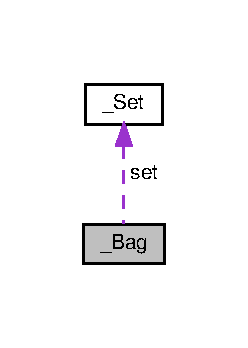
\includegraphics[width=119pt]{struct__Bag__coll__graph}
\end{center}
\end{figure}
\subsection*{Data Fields}
\begin{DoxyCompactItemize}
\item 
\mbox{\Hypertarget{struct__Bag_a07df3f3b358ee3a3f65223f25a4565f6}\label{struct__Bag_a07df3f3b358ee3a3f65223f25a4565f6}} 
\hyperlink{set_8h_a6d3b7f7c92cbb4577ef3ef7ddbf93161}{Set} $\ast$ \hyperlink{struct__Bag_a07df3f3b358ee3a3f65223f25a4565f6}{set}
\begin{DoxyCompactList}\small\item\em defines set \end{DoxyCompactList}\item 
\mbox{\Hypertarget{struct__Bag_ad644d22c425628ddeb1a7c6da0a0fdeb}\label{struct__Bag_ad644d22c425628ddeb1a7c6da0a0fdeb}} 
int \hyperlink{struct__Bag_ad644d22c425628ddeb1a7c6da0a0fdeb}{max\+\_\+obj}
\begin{DoxyCompactList}\small\item\em defines max objects \end{DoxyCompactList}\end{DoxyCompactItemize}


\subsection{Detailed Description}
defines structure of bag 

The documentation for this struct was generated from the following file\+:\begin{DoxyCompactItemize}
\item 
\hyperlink{inventory_8c}{inventory.\+c}\end{DoxyCompactItemize}

\hypertarget{struct__Dialogue}{\section{\+\_\+\+Dialogue Struct Reference}
\label{struct__Dialogue}\index{\+\_\+\+Dialogue@{\+\_\+\+Dialogue}}
}


Estructura del dialogue.  




Collaboration diagram for \+\_\+\+Dialogue\+:
\nopagebreak
\begin{figure}[H]
\begin{center}
\leavevmode
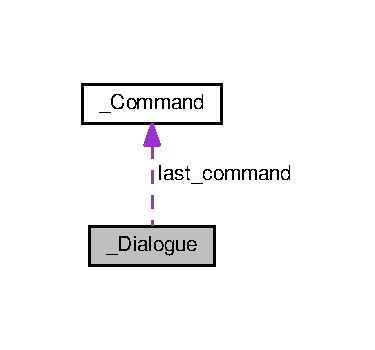
\includegraphics[width=180pt]{struct__Dialogue__coll__graph}
\end{center}
\end{figure}
\subsection*{Public Attributes}
\begin{DoxyCompactItemize}
\item 
int \hyperlink{struct__Dialogue_a36b7548a4853c80dd35fe7feb6e21252}{repeat}
\item 
\hyperlink{command_8h_a7d2935971c252377cb0fc1c8545dc2bc}{Command} $\ast$ \hyperlink{struct__Dialogue_ad4340f1881243b083535594a283a864b}{last\+\_\+command}
\item 
\hyperlink{command_8h_a0473597db8c45c0289b6b8e2f8abbe32}{T\+\_\+\+Command} \hyperlink{struct__Dialogue_a5916cc0658d2489b07e4c07d1af9029f}{previous\+\_\+command}
\item 
char \hyperlink{struct__Dialogue_a469e24b5ab5ee38a4219889a45c607a0}{previous\+\_\+command\+\_\+name} \mbox{[}\hyperlink{types_8h_a92ed8507d1cd2331ad09275c5c4c1c89}{W\+O\+R\+D\+\_\+\+S\+I\+Z\+E}\mbox{]}
\item 
\hyperlink{types_8h_a32c27cc471df37f4fc818d65de0a56c4}{S\+T\+A\+T\+U\+S} \hyperlink{struct__Dialogue_af479d1df9a92c3233bfaaa3dd332520e}{status\+\_\+command}
\item 
\hyperlink{types_8h_a3e5b8192e7d9ffaf3542f1210aec18dd}{B\+O\+O\+L} \hyperlink{struct__Dialogue_a273106296bef7851f910cbd8ace3c16d}{status\+\_\+link}
\item 
\hyperlink{types_8h_a3e5b8192e7d9ffaf3542f1210aec18dd}{B\+O\+O\+L} \hyperlink{struct__Dialogue_a877e735a7c75ad25838756e50ca8341e}{status\+\_\+object}
\item 
\hyperlink{types_8h_a3e5b8192e7d9ffaf3542f1210aec18dd}{B\+O\+O\+L} \hyperlink{struct__Dialogue_aef9641ab92321bf3b59362c8cbb5dad1}{status\+\_\+space}
\item 
\hyperlink{types_8h_a3e5b8192e7d9ffaf3542f1210aec18dd}{B\+O\+O\+L} \hyperlink{struct__Dialogue_a2334a9bb36055478553f576db1c91a54}{link\+\_\+already\+\_\+open}
\item 
\hyperlink{types_8h_a3e5b8192e7d9ffaf3542f1210aec18dd}{B\+O\+O\+L} \hyperlink{struct__Dialogue_ab41d3ec815fc544944f1edb5e9f158a6}{no\+\_\+monster}
\item 
char \hyperlink{struct__Dialogue_a423dddb02d061194426cdde84f1ccf95}{object} \mbox{[}\hyperlink{types_8h_a92ed8507d1cd2331ad09275c5c4c1c89}{W\+O\+R\+D\+\_\+\+S\+I\+Z\+E}\mbox{]}
\item 
char \hyperlink{struct__Dialogue_adfdfa42510a4f6bccc37d7250529574d}{link} \mbox{[}\hyperlink{types_8h_a92ed8507d1cd2331ad09275c5c4c1c89}{W\+O\+R\+D\+\_\+\+S\+I\+Z\+E}\mbox{]}
\item 
char \hyperlink{struct__Dialogue_a28fdc6bd5c84508d271bf9464245f731}{space} \mbox{[}\hyperlink{types_8h_a92ed8507d1cd2331ad09275c5c4c1c89}{W\+O\+R\+D\+\_\+\+S\+I\+Z\+E}\mbox{]}
\item 
char \hyperlink{struct__Dialogue_a6d5e37264cf94fb53c0eb66f796b5705}{text} \mbox{[}\hyperlink{types_8h_a92ed8507d1cd2331ad09275c5c4c1c89}{W\+O\+R\+D\+\_\+\+S\+I\+Z\+E}\mbox{]}
\end{DoxyCompactItemize}


\subsection{Detailed Description}
Estructura del dialogue. 

\subsection{Member Data Documentation}
\hypertarget{struct__Dialogue_ad4340f1881243b083535594a283a864b}{\index{\+\_\+\+Dialogue@{\+\_\+\+Dialogue}!last\+\_\+command@{last\+\_\+command}}
\index{last\+\_\+command@{last\+\_\+command}!\+\_\+\+Dialogue@{\+\_\+\+Dialogue}}
\subsubsection[{last\+\_\+command}]{\setlength{\rightskip}{0pt plus 5cm}{\bf Command}$\ast$ \+\_\+\+Dialogue\+::last\+\_\+command}}\label{struct__Dialogue_ad4340f1881243b083535594a283a864b}
Comando anterior \hypertarget{struct__Dialogue_adfdfa42510a4f6bccc37d7250529574d}{\index{\+\_\+\+Dialogue@{\+\_\+\+Dialogue}!link@{link}}
\index{link@{link}!\+\_\+\+Dialogue@{\+\_\+\+Dialogue}}
\subsubsection[{link}]{\setlength{\rightskip}{0pt plus 5cm}char \+\_\+\+Dialogue\+::link\mbox{[}{\bf W\+O\+R\+D\+\_\+\+S\+I\+Z\+E}\mbox{]}}}\label{struct__Dialogue_adfdfa42510a4f6bccc37d7250529574d}
Nombre del link \hypertarget{struct__Dialogue_a2334a9bb36055478553f576db1c91a54}{\index{\+\_\+\+Dialogue@{\+\_\+\+Dialogue}!link\+\_\+already\+\_\+open@{link\+\_\+already\+\_\+open}}
\index{link\+\_\+already\+\_\+open@{link\+\_\+already\+\_\+open}!\+\_\+\+Dialogue@{\+\_\+\+Dialogue}}
\subsubsection[{link\+\_\+already\+\_\+open}]{\setlength{\rightskip}{0pt plus 5cm}{\bf B\+O\+O\+L} \+\_\+\+Dialogue\+::link\+\_\+already\+\_\+open}}\label{struct__Dialogue_a2334a9bb36055478553f576db1c91a54}
Para indicar que un link ya esta abierto \hypertarget{struct__Dialogue_ab41d3ec815fc544944f1edb5e9f158a6}{\index{\+\_\+\+Dialogue@{\+\_\+\+Dialogue}!no\+\_\+monster@{no\+\_\+monster}}
\index{no\+\_\+monster@{no\+\_\+monster}!\+\_\+\+Dialogue@{\+\_\+\+Dialogue}}
\subsubsection[{no\+\_\+monster}]{\setlength{\rightskip}{0pt plus 5cm}{\bf B\+O\+O\+L} \+\_\+\+Dialogue\+::no\+\_\+monster}}\label{struct__Dialogue_ab41d3ec815fc544944f1edb5e9f158a6}
Para indicar que no se puede luchar con el monstruo porque no esta ahí \hypertarget{struct__Dialogue_a423dddb02d061194426cdde84f1ccf95}{\index{\+\_\+\+Dialogue@{\+\_\+\+Dialogue}!object@{object}}
\index{object@{object}!\+\_\+\+Dialogue@{\+\_\+\+Dialogue}}
\subsubsection[{object}]{\setlength{\rightskip}{0pt plus 5cm}char \+\_\+\+Dialogue\+::object\mbox{[}{\bf W\+O\+R\+D\+\_\+\+S\+I\+Z\+E}\mbox{]}}}\label{struct__Dialogue_a423dddb02d061194426cdde84f1ccf95}
Nombre del objeto \hypertarget{struct__Dialogue_a5916cc0658d2489b07e4c07d1af9029f}{\index{\+\_\+\+Dialogue@{\+\_\+\+Dialogue}!previous\+\_\+command@{previous\+\_\+command}}
\index{previous\+\_\+command@{previous\+\_\+command}!\+\_\+\+Dialogue@{\+\_\+\+Dialogue}}
\subsubsection[{previous\+\_\+command}]{\setlength{\rightskip}{0pt plus 5cm}{\bf T\+\_\+\+Command} \+\_\+\+Dialogue\+::previous\+\_\+command}}\label{struct__Dialogue_a5916cc0658d2489b07e4c07d1af9029f}
Tipo de comando anterior \hypertarget{struct__Dialogue_a469e24b5ab5ee38a4219889a45c607a0}{\index{\+\_\+\+Dialogue@{\+\_\+\+Dialogue}!previous\+\_\+command\+\_\+name@{previous\+\_\+command\+\_\+name}}
\index{previous\+\_\+command\+\_\+name@{previous\+\_\+command\+\_\+name}!\+\_\+\+Dialogue@{\+\_\+\+Dialogue}}
\subsubsection[{previous\+\_\+command\+\_\+name}]{\setlength{\rightskip}{0pt plus 5cm}char \+\_\+\+Dialogue\+::previous\+\_\+command\+\_\+name\mbox{[}{\bf W\+O\+R\+D\+\_\+\+S\+I\+Z\+E}\mbox{]}}}\label{struct__Dialogue_a469e24b5ab5ee38a4219889a45c607a0}
Nombre del comando anterior \hypertarget{struct__Dialogue_a36b7548a4853c80dd35fe7feb6e21252}{\index{\+\_\+\+Dialogue@{\+\_\+\+Dialogue}!repeat@{repeat}}
\index{repeat@{repeat}!\+\_\+\+Dialogue@{\+\_\+\+Dialogue}}
\subsubsection[{repeat}]{\setlength{\rightskip}{0pt plus 5cm}int \+\_\+\+Dialogue\+::repeat}}\label{struct__Dialogue_a36b7548a4853c80dd35fe7feb6e21252}
Contador de repeticiones \hypertarget{struct__Dialogue_a28fdc6bd5c84508d271bf9464245f731}{\index{\+\_\+\+Dialogue@{\+\_\+\+Dialogue}!space@{space}}
\index{space@{space}!\+\_\+\+Dialogue@{\+\_\+\+Dialogue}}
\subsubsection[{space}]{\setlength{\rightskip}{0pt plus 5cm}char \+\_\+\+Dialogue\+::space\mbox{[}{\bf W\+O\+R\+D\+\_\+\+S\+I\+Z\+E}\mbox{]}}}\label{struct__Dialogue_a28fdc6bd5c84508d271bf9464245f731}
Nombre del espacio al que llegamos \hypertarget{struct__Dialogue_af479d1df9a92c3233bfaaa3dd332520e}{\index{\+\_\+\+Dialogue@{\+\_\+\+Dialogue}!status\+\_\+command@{status\+\_\+command}}
\index{status\+\_\+command@{status\+\_\+command}!\+\_\+\+Dialogue@{\+\_\+\+Dialogue}}
\subsubsection[{status\+\_\+command}]{\setlength{\rightskip}{0pt plus 5cm}{\bf S\+T\+A\+T\+U\+S} \+\_\+\+Dialogue\+::status\+\_\+command}}\label{struct__Dialogue_af479d1df9a92c3233bfaaa3dd332520e}
Si se ha hecho la accion \hypertarget{struct__Dialogue_a273106296bef7851f910cbd8ace3c16d}{\index{\+\_\+\+Dialogue@{\+\_\+\+Dialogue}!status\+\_\+link@{status\+\_\+link}}
\index{status\+\_\+link@{status\+\_\+link}!\+\_\+\+Dialogue@{\+\_\+\+Dialogue}}
\subsubsection[{status\+\_\+link}]{\setlength{\rightskip}{0pt plus 5cm}{\bf B\+O\+O\+L} \+\_\+\+Dialogue\+::status\+\_\+link}}\label{struct__Dialogue_a273106296bef7851f910cbd8ace3c16d}
Para indicar si el link esta cerrado \hypertarget{struct__Dialogue_a877e735a7c75ad25838756e50ca8341e}{\index{\+\_\+\+Dialogue@{\+\_\+\+Dialogue}!status\+\_\+object@{status\+\_\+object}}
\index{status\+\_\+object@{status\+\_\+object}!\+\_\+\+Dialogue@{\+\_\+\+Dialogue}}
\subsubsection[{status\+\_\+object}]{\setlength{\rightskip}{0pt plus 5cm}{\bf B\+O\+O\+L} \+\_\+\+Dialogue\+::status\+\_\+object}}\label{struct__Dialogue_a877e735a7c75ad25838756e50ca8341e}
Para indicar que es un objeto no movible \hypertarget{struct__Dialogue_aef9641ab92321bf3b59362c8cbb5dad1}{\index{\+\_\+\+Dialogue@{\+\_\+\+Dialogue}!status\+\_\+space@{status\+\_\+space}}
\index{status\+\_\+space@{status\+\_\+space}!\+\_\+\+Dialogue@{\+\_\+\+Dialogue}}
\subsubsection[{status\+\_\+space}]{\setlength{\rightskip}{0pt plus 5cm}{\bf B\+O\+O\+L} \+\_\+\+Dialogue\+::status\+\_\+space}}\label{struct__Dialogue_aef9641ab92321bf3b59362c8cbb5dad1}
Para indicar que lo que se checkea es un espacio \hypertarget{struct__Dialogue_a6d5e37264cf94fb53c0eb66f796b5705}{\index{\+\_\+\+Dialogue@{\+\_\+\+Dialogue}!text@{text}}
\index{text@{text}!\+\_\+\+Dialogue@{\+\_\+\+Dialogue}}
\subsubsection[{text}]{\setlength{\rightskip}{0pt plus 5cm}char \+\_\+\+Dialogue\+::text\mbox{[}{\bf W\+O\+R\+D\+\_\+\+S\+I\+Z\+E}\mbox{]}}}\label{struct__Dialogue_a6d5e37264cf94fb53c0eb66f796b5705}
Texto del respuesta del dialogue 

The documentation for this struct was generated from the following file\+:\begin{DoxyCompactItemize}
\item 
src/\hyperlink{dialogue_8c}{dialogue.\+c}\end{DoxyCompactItemize}

\hypertarget{struct__Die}{\section{\+\_\+\+Die Struct Reference}
\label{struct__Die}\index{\+\_\+\+Die@{\+\_\+\+Die}}
}


Estructura del die.  


\subsection*{Public Attributes}
\begin{DoxyCompactItemize}
\item 
\hyperlink{types_8h_a845e604fb28f7e3d97549da3448149d3}{Id} \hyperlink{struct__Die_a0887af562dda760409957f13619d36f1}{id}
\item 
int \hyperlink{struct__Die_a32eb6d76a658d00832c484818879d071}{last\+\_\+num}
\end{DoxyCompactItemize}


\subsection{Detailed Description}
Estructura del die. 

\subsection{Member Data Documentation}
\hypertarget{struct__Die_a0887af562dda760409957f13619d36f1}{\index{\+\_\+\+Die@{\+\_\+\+Die}!id@{id}}
\index{id@{id}!\+\_\+\+Die@{\+\_\+\+Die}}
\subsubsection[{id}]{\setlength{\rightskip}{0pt plus 5cm}{\bf Id} \+\_\+\+Die\+::id}}\label{struct__Die_a0887af562dda760409957f13619d36f1}
Identificador del dado \hypertarget{struct__Die_a32eb6d76a658d00832c484818879d071}{\index{\+\_\+\+Die@{\+\_\+\+Die}!last\+\_\+num@{last\+\_\+num}}
\index{last\+\_\+num@{last\+\_\+num}!\+\_\+\+Die@{\+\_\+\+Die}}
\subsubsection[{last\+\_\+num}]{\setlength{\rightskip}{0pt plus 5cm}int \+\_\+\+Die\+::last\+\_\+num}}\label{struct__Die_a32eb6d76a658d00832c484818879d071}
Ultimo número del dado 

The documentation for this struct was generated from the following file\+:\begin{DoxyCompactItemize}
\item 
src/\hyperlink{die_8c}{die.\+c}\end{DoxyCompactItemize}

\hypertarget{struct__Game}{}\section{\+\_\+\+Game Struct Reference}
\label{struct__Game}\index{\+\_\+\+Game@{\+\_\+\+Game}}


defines structure of game  




Collaboration diagram for \+\_\+\+Game\+:
\nopagebreak
\begin{figure}[H]
\begin{center}
\leavevmode
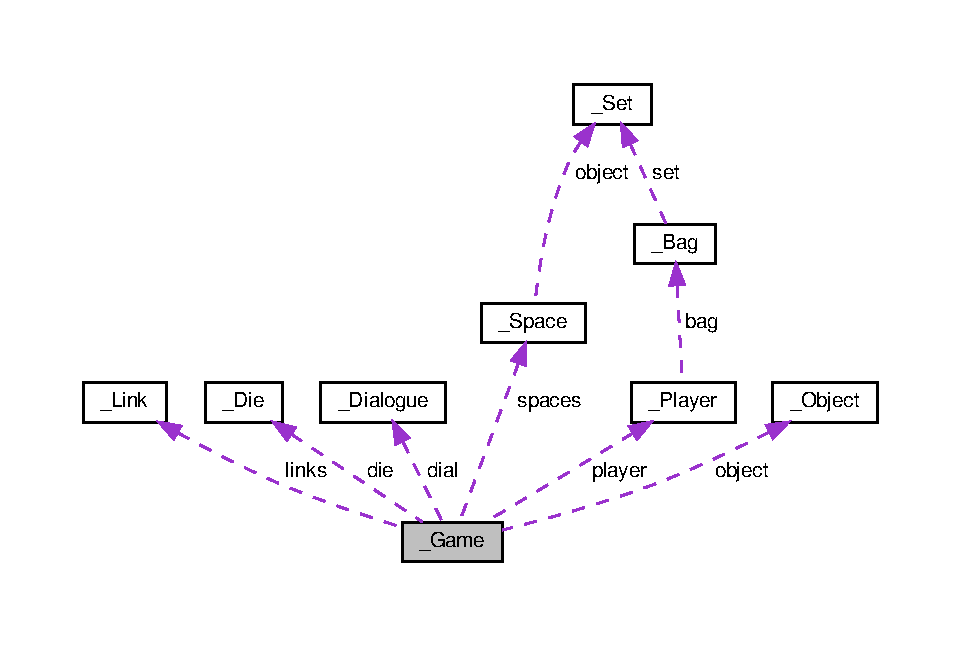
\includegraphics[width=350pt]{struct__Game__coll__graph}
\end{center}
\end{figure}
\subsection*{Data Fields}
\begin{DoxyCompactItemize}
\item 
\mbox{\Hypertarget{struct__Game_a880e48b4441e503a9ac070901c19b623}\label{struct__Game_a880e48b4441e503a9ac070901c19b623}} 
\hyperlink{object_8h_a7f8bbcda919b65ce67f92fba08e0212f}{Object} $\ast$ \hyperlink{struct__Game_a880e48b4441e503a9ac070901c19b623}{object} \mbox{[}\hyperlink{set_8h_a0ffebf572977a670aba207757c157eba}{M\+A\+X\+\_\+\+I\+Ds\+\_\+\+S\+ET}\mbox{]}
\begin{DoxyCompactList}\small\item\em defines array of object \end{DoxyCompactList}\item 
\mbox{\Hypertarget{struct__Game_a31406605782d71ec00c4bf258ea76267}\label{struct__Game_a31406605782d71ec00c4bf258ea76267}} 
\hyperlink{player_8h_af30e2030635a69690f85e48bc6ef202f}{Player} $\ast$ \hyperlink{struct__Game_a31406605782d71ec00c4bf258ea76267}{player}
\begin{DoxyCompactList}\small\item\em defines pointer to player \end{DoxyCompactList}\item 
\mbox{\Hypertarget{struct__Game_ab4180417d9148f8abb2233ca6c4ecfe5}\label{struct__Game_ab4180417d9148f8abb2233ca6c4ecfe5}} 
\hyperlink{space_8h_a67533ffc2b70463baecc38fb0629bbfc}{Space} $\ast$ \hyperlink{struct__Game_ab4180417d9148f8abb2233ca6c4ecfe5}{spaces} \mbox{[}\hyperlink{space_8h_a5f54fd55f983a2e33ce076cd9f587e82}{M\+A\+X\+\_\+\+S\+P\+A\+C\+ES}+1\mbox{]}
\begin{DoxyCompactList}\small\item\em defines pointer to array of spaces \end{DoxyCompactList}\item 
\mbox{\Hypertarget{struct__Game_a27727b50ea0904a1fe9e1c55c27f2cf1}\label{struct__Game_a27727b50ea0904a1fe9e1c55c27f2cf1}} 
\hyperlink{command_8h_a0473597db8c45c0289b6b8e2f8abbe32}{T\+\_\+\+Command} \hyperlink{struct__Game_a27727b50ea0904a1fe9e1c55c27f2cf1}{last\+\_\+cmd}
\begin{DoxyCompactList}\small\item\em defines last\+\_\+cmd \end{DoxyCompactList}\item 
\mbox{\Hypertarget{struct__Game_aea7cfcbda905e1b3ce6f9b3542b7d6cc}\label{struct__Game_aea7cfcbda905e1b3ce6f9b3542b7d6cc}} 
\hyperlink{types_8h_a32c27cc471df37f4fc818d65de0a56c4}{S\+T\+A\+T\+US} \hyperlink{struct__Game_aea7cfcbda905e1b3ce6f9b3542b7d6cc}{cmd\+\_\+status}
\begin{DoxyCompactList}\small\item\em defines cmd\+\_\+status \end{DoxyCompactList}\item 
\mbox{\Hypertarget{struct__Game_a0d6009b5dcb080489c192a9198fa7d46}\label{struct__Game_a0d6009b5dcb080489c192a9198fa7d46}} 
\hyperlink{die_8h_a892f0b0bf81d69a1f7a14ea238e36dd3}{Die} $\ast$ \hyperlink{struct__Game_a0d6009b5dcb080489c192a9198fa7d46}{die}
\begin{DoxyCompactList}\small\item\em defines pointer to die \end{DoxyCompactList}\item 
\mbox{\Hypertarget{struct__Game_ad0fa85f42aa7e8a7d560312c80988776}\label{struct__Game_ad0fa85f42aa7e8a7d560312c80988776}} 
char \hyperlink{struct__Game_ad0fa85f42aa7e8a7d560312c80988776}{objdsc} \mbox{[}\hyperlink{types_8h_a92ed8507d1cd2331ad09275c5c4c1c89}{W\+O\+R\+D\+\_\+\+S\+I\+ZE}+1\mbox{]}
\begin{DoxyCompactList}\small\item\em definesarray of objdsc \end{DoxyCompactList}\item 
\mbox{\Hypertarget{struct__Game_ac2e1dc07e9d2ad410d1c16bc83ba5101}\label{struct__Game_ac2e1dc07e9d2ad410d1c16bc83ba5101}} 
\hyperlink{link_8h_ae3b299941e67be6971bfd64a25505eff}{Link} $\ast$ \hyperlink{struct__Game_ac2e1dc07e9d2ad410d1c16bc83ba5101}{links} \mbox{[}\hyperlink{space_8h_a5f54fd55f983a2e33ce076cd9f587e82}{M\+A\+X\+\_\+\+S\+P\+A\+C\+ES}+1\mbox{]}
\begin{DoxyCompactList}\small\item\em defines array of links \end{DoxyCompactList}\end{DoxyCompactItemize}


\subsection{Detailed Description}
defines structure of game 

The documentation for this struct was generated from the following file\+:\begin{DoxyCompactItemize}
\item 
\hyperlink{game_8c}{game.\+c}\end{DoxyCompactItemize}

\hypertarget{struct__Graphic__engine}{}\section{\+\_\+\+Graphic\+\_\+engine Struct Reference}
\label{struct__Graphic__engine}\index{\+\_\+\+Graphic\+\_\+engine@{\+\_\+\+Graphic\+\_\+engine}}


defines structure of graphic engine  




Collaboration diagram for \+\_\+\+Graphic\+\_\+engine\+:
\nopagebreak
\begin{figure}[H]
\begin{center}
\leavevmode
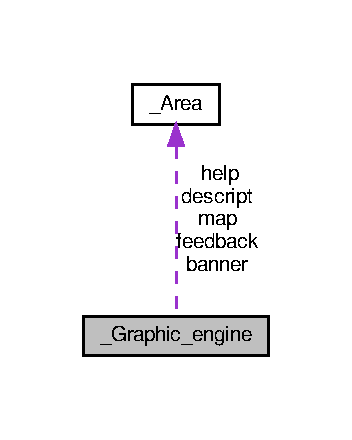
\includegraphics[width=169pt]{struct__Graphic__engine__coll__graph}
\end{center}
\end{figure}
\subsection*{Data Fields}
\begin{DoxyCompactItemize}
\item 
\mbox{\Hypertarget{struct__Graphic__engine_a1ea06bb881d335da8c31d63b3e834bdb}\label{struct__Graphic__engine_a1ea06bb881d335da8c31d63b3e834bdb}} 
\hyperlink{screen_8h_acfdfc42f6522d75fa3c16713afde8127}{Area} $\ast$ \hyperlink{struct__Graphic__engine_a1ea06bb881d335da8c31d63b3e834bdb}{map}
\begin{DoxyCompactList}\small\item\em defines the area of map \end{DoxyCompactList}\item 
\mbox{\Hypertarget{struct__Graphic__engine_a414bb888ecce3389c7ce348264758e58}\label{struct__Graphic__engine_a414bb888ecce3389c7ce348264758e58}} 
\hyperlink{screen_8h_acfdfc42f6522d75fa3c16713afde8127}{Area} $\ast$ \hyperlink{struct__Graphic__engine_a414bb888ecce3389c7ce348264758e58}{descript}
\begin{DoxyCompactList}\small\item\em defines the area of descript \end{DoxyCompactList}\item 
\mbox{\Hypertarget{struct__Graphic__engine_a440dfb2c23c3c4b7d3871187371117b9}\label{struct__Graphic__engine_a440dfb2c23c3c4b7d3871187371117b9}} 
\hyperlink{screen_8h_acfdfc42f6522d75fa3c16713afde8127}{Area} $\ast$ \hyperlink{struct__Graphic__engine_a440dfb2c23c3c4b7d3871187371117b9}{banner}
\begin{DoxyCompactList}\small\item\em defines the area of banner \end{DoxyCompactList}\item 
\mbox{\Hypertarget{struct__Graphic__engine_ade1d3e95ad6def427f613a4a2d101875}\label{struct__Graphic__engine_ade1d3e95ad6def427f613a4a2d101875}} 
\hyperlink{screen_8h_acfdfc42f6522d75fa3c16713afde8127}{Area} $\ast$ \hyperlink{struct__Graphic__engine_ade1d3e95ad6def427f613a4a2d101875}{help}
\begin{DoxyCompactList}\small\item\em defines the area of help \end{DoxyCompactList}\item 
\mbox{\Hypertarget{struct__Graphic__engine_a4fc0ef353d000b20d57fb75d898c6d2d}\label{struct__Graphic__engine_a4fc0ef353d000b20d57fb75d898c6d2d}} 
\hyperlink{screen_8h_acfdfc42f6522d75fa3c16713afde8127}{Area} $\ast$ \hyperlink{struct__Graphic__engine_a4fc0ef353d000b20d57fb75d898c6d2d}{feedback}
\begin{DoxyCompactList}\small\item\em defines the area of feedback \end{DoxyCompactList}\end{DoxyCompactItemize}


\subsection{Detailed Description}
defines structure of graphic engine 

The documentation for this struct was generated from the following file\+:\begin{DoxyCompactItemize}
\item 
\hyperlink{graphic__engine_8c}{graphic\+\_\+engine.\+c}\end{DoxyCompactItemize}

\hypertarget{struct__Link}{\section{\+\_\+\+Link Struct Reference}
\label{struct__Link}\index{\+\_\+\+Link@{\+\_\+\+Link}}
}


Estructura del link.  


\subsection*{Public Attributes}
\begin{DoxyCompactItemize}
\item 
\hyperlink{types_8h_a845e604fb28f7e3d97549da3448149d3}{Id} \hyperlink{struct__Link_a151212e7a8e8274c2a1ee991ba95878b}{id}
\item 
\hyperlink{types_8h_a845e604fb28f7e3d97549da3448149d3}{Id} \hyperlink{struct__Link_a05724c89a2945c364f76302d1bcd3196}{spaces} \mbox{[}L\+I\+N\+K\+\_\+\+S\+P\+A\+C\+E\+S\mbox{]}
\item 
char \hyperlink{struct__Link_a655f0a5d235d1fd6797299dd4763672b}{name} \mbox{[}\hyperlink{types_8h_a92ed8507d1cd2331ad09275c5c4c1c89}{W\+O\+R\+D\+\_\+\+S\+I\+Z\+E}\mbox{]}
\item 
\hyperlink{types_8h_a4eb959f56c9de4fb79f4891902033093}{D\+O\+O\+R} \hyperlink{struct__Link_a4d1168b16e3b3c297a6e7b096ff8b9f7}{status}
\end{DoxyCompactItemize}


\subsection{Detailed Description}
Estructura del link. 

\subsection{Member Data Documentation}
\hypertarget{struct__Link_a151212e7a8e8274c2a1ee991ba95878b}{\index{\+\_\+\+Link@{\+\_\+\+Link}!id@{id}}
\index{id@{id}!\+\_\+\+Link@{\+\_\+\+Link}}
\subsubsection[{id}]{\setlength{\rightskip}{0pt plus 5cm}{\bf Id} \+\_\+\+Link\+::id}}\label{struct__Link_a151212e7a8e8274c2a1ee991ba95878b}
Identificador del link \hypertarget{struct__Link_a655f0a5d235d1fd6797299dd4763672b}{\index{\+\_\+\+Link@{\+\_\+\+Link}!name@{name}}
\index{name@{name}!\+\_\+\+Link@{\+\_\+\+Link}}
\subsubsection[{name}]{\setlength{\rightskip}{0pt plus 5cm}char \+\_\+\+Link\+::name\mbox{[}{\bf W\+O\+R\+D\+\_\+\+S\+I\+Z\+E}\mbox{]}}}\label{struct__Link_a655f0a5d235d1fd6797299dd4763672b}
Nombre del enlace \hypertarget{struct__Link_a05724c89a2945c364f76302d1bcd3196}{\index{\+\_\+\+Link@{\+\_\+\+Link}!spaces@{spaces}}
\index{spaces@{spaces}!\+\_\+\+Link@{\+\_\+\+Link}}
\subsubsection[{spaces}]{\setlength{\rightskip}{0pt plus 5cm}{\bf Id} \+\_\+\+Link\+::spaces\mbox{[}L\+I\+N\+K\+\_\+\+S\+P\+A\+C\+E\+S\mbox{]}}}\label{struct__Link_a05724c89a2945c364f76302d1bcd3196}
Identificadores de los espacios \hypertarget{struct__Link_a4d1168b16e3b3c297a6e7b096ff8b9f7}{\index{\+\_\+\+Link@{\+\_\+\+Link}!status@{status}}
\index{status@{status}!\+\_\+\+Link@{\+\_\+\+Link}}
\subsubsection[{status}]{\setlength{\rightskip}{0pt plus 5cm}{\bf D\+O\+O\+R} \+\_\+\+Link\+::status}}\label{struct__Link_a4d1168b16e3b3c297a6e7b096ff8b9f7}
Estado del enlace 

The documentation for this struct was generated from the following file\+:\begin{DoxyCompactItemize}
\item 
src/\hyperlink{link_8c}{link.\+c}\end{DoxyCompactItemize}

\hypertarget{struct__Object}{\section{\+\_\+\+Object Struct Reference}
\label{struct__Object}\index{\+\_\+\+Object@{\+\_\+\+Object}}
}


Estructura del objeto.  


\subsection*{Public Attributes}
\begin{DoxyCompactItemize}
\item 
\hyperlink{types_8h_a845e604fb28f7e3d97549da3448149d3}{Id} \hyperlink{struct__Object_a3cff7a0e8dc4e9d23895ed9af1b7653a}{id}
\item 
\hyperlink{types_8h_a845e604fb28f7e3d97549da3448149d3}{Id} \hyperlink{struct__Object_a42b5cf094a2df1756303245ea70dbb55}{pos\+\_\+original}
\item 
char \hyperlink{struct__Object_a3dab853826b88558a2c07dec50b96d57}{name} \mbox{[}\hyperlink{types_8h_a92ed8507d1cd2331ad09275c5c4c1c89}{W\+O\+R\+D\+\_\+\+S\+I\+Z\+E}\mbox{]}
\item 
char \hyperlink{struct__Object_a556e2e37c1461bcaae6492d2101f407d}{description} \mbox{[}\hyperlink{types_8h_a92ed8507d1cd2331ad09275c5c4c1c89}{W\+O\+R\+D\+\_\+\+S\+I\+Z\+E}\mbox{]}
\item 
char \hyperlink{struct__Object_a786e4c903e42b20ed785fbe4372941e0}{des\+\_\+movido} \mbox{[}\hyperlink{types_8h_a92ed8507d1cd2331ad09275c5c4c1c89}{W\+O\+R\+D\+\_\+\+S\+I\+Z\+E}\mbox{]}
\item 
\hyperlink{types_8h_a3e5b8192e7d9ffaf3542f1210aec18dd}{B\+O\+O\+L} \hyperlink{struct__Object_a182b654831db35840643f7ac44dba937}{movible}
\item 
\hyperlink{types_8h_a3e5b8192e7d9ffaf3542f1210aec18dd}{B\+O\+O\+L} \hyperlink{struct__Object_aa2e3f6d7b7b8e2ed9b42b550650dd1e5}{movido}
\item 
\hyperlink{types_8h_a3e5b8192e7d9ffaf3542f1210aec18dd}{B\+O\+O\+L} \hyperlink{struct__Object_ae80a5867852e78b0c158844c280b2d5a}{oculto}
\item 
\hyperlink{types_8h_a845e604fb28f7e3d97549da3448149d3}{Id} \hyperlink{struct__Object_a0922dd9891e6aa617ce1d51ae27c0175}{open}
\item 
\hyperlink{types_8h_a3e5b8192e7d9ffaf3542f1210aec18dd}{B\+O\+O\+L} \hyperlink{struct__Object_afcf4d46d3327646477e5e70bb0535653}{iluminado}
\item 
\hyperlink{types_8h_a3e5b8192e7d9ffaf3542f1210aec18dd}{B\+O\+O\+L} \hyperlink{struct__Object_a69dc115b72581c6618dd7c0d860d4c04}{encendido}
\end{DoxyCompactItemize}


\subsection{Detailed Description}
Estructura del objeto. 

\subsection{Member Data Documentation}
\hypertarget{struct__Object_a786e4c903e42b20ed785fbe4372941e0}{\index{\+\_\+\+Object@{\+\_\+\+Object}!des\+\_\+movido@{des\+\_\+movido}}
\index{des\+\_\+movido@{des\+\_\+movido}!\+\_\+\+Object@{\+\_\+\+Object}}
\subsubsection[{des\+\_\+movido}]{\setlength{\rightskip}{0pt plus 5cm}char \+\_\+\+Object\+::des\+\_\+movido\mbox{[}{\bf W\+O\+R\+D\+\_\+\+S\+I\+Z\+E}\mbox{]}}}\label{struct__Object_a786e4c903e42b20ed785fbe4372941e0}
Descripcion del objeto movido. \hypertarget{struct__Object_a556e2e37c1461bcaae6492d2101f407d}{\index{\+\_\+\+Object@{\+\_\+\+Object}!description@{description}}
\index{description@{description}!\+\_\+\+Object@{\+\_\+\+Object}}
\subsubsection[{description}]{\setlength{\rightskip}{0pt plus 5cm}char \+\_\+\+Object\+::description\mbox{[}{\bf W\+O\+R\+D\+\_\+\+S\+I\+Z\+E}\mbox{]}}}\label{struct__Object_a556e2e37c1461bcaae6492d2101f407d}
Descripcion del objeto pos inicial \hypertarget{struct__Object_a69dc115b72581c6618dd7c0d860d4c04}{\index{\+\_\+\+Object@{\+\_\+\+Object}!encendido@{encendido}}
\index{encendido@{encendido}!\+\_\+\+Object@{\+\_\+\+Object}}
\subsubsection[{encendido}]{\setlength{\rightskip}{0pt plus 5cm}{\bf B\+O\+O\+L} \+\_\+\+Object\+::encendido}}\label{struct__Object_a69dc115b72581c6618dd7c0d860d4c04}
Objecto encendido o no \hypertarget{struct__Object_a3cff7a0e8dc4e9d23895ed9af1b7653a}{\index{\+\_\+\+Object@{\+\_\+\+Object}!id@{id}}
\index{id@{id}!\+\_\+\+Object@{\+\_\+\+Object}}
\subsubsection[{id}]{\setlength{\rightskip}{0pt plus 5cm}{\bf Id} \+\_\+\+Object\+::id}}\label{struct__Object_a3cff7a0e8dc4e9d23895ed9af1b7653a}
identificador del objeto. \hypertarget{struct__Object_afcf4d46d3327646477e5e70bb0535653}{\index{\+\_\+\+Object@{\+\_\+\+Object}!iluminado@{iluminado}}
\index{iluminado@{iluminado}!\+\_\+\+Object@{\+\_\+\+Object}}
\subsubsection[{iluminado}]{\setlength{\rightskip}{0pt plus 5cm}{\bf B\+O\+O\+L} \+\_\+\+Object\+::iluminado}}\label{struct__Object_afcf4d46d3327646477e5e70bb0535653}
Objecto puede iluminar o no \hypertarget{struct__Object_a182b654831db35840643f7ac44dba937}{\index{\+\_\+\+Object@{\+\_\+\+Object}!movible@{movible}}
\index{movible@{movible}!\+\_\+\+Object@{\+\_\+\+Object}}
\subsubsection[{movible}]{\setlength{\rightskip}{0pt plus 5cm}{\bf B\+O\+O\+L} \+\_\+\+Object\+::movible}}\label{struct__Object_a182b654831db35840643f7ac44dba937}
Objecto movible o no \hypertarget{struct__Object_aa2e3f6d7b7b8e2ed9b42b550650dd1e5}{\index{\+\_\+\+Object@{\+\_\+\+Object}!movido@{movido}}
\index{movido@{movido}!\+\_\+\+Object@{\+\_\+\+Object}}
\subsubsection[{movido}]{\setlength{\rightskip}{0pt plus 5cm}{\bf B\+O\+O\+L} \+\_\+\+Object\+::movido}}\label{struct__Object_aa2e3f6d7b7b8e2ed9b42b550650dd1e5}
Objeto ha sido movido. \hypertarget{struct__Object_a3dab853826b88558a2c07dec50b96d57}{\index{\+\_\+\+Object@{\+\_\+\+Object}!name@{name}}
\index{name@{name}!\+\_\+\+Object@{\+\_\+\+Object}}
\subsubsection[{name}]{\setlength{\rightskip}{0pt plus 5cm}char \+\_\+\+Object\+::name\mbox{[}{\bf W\+O\+R\+D\+\_\+\+S\+I\+Z\+E}\mbox{]}}}\label{struct__Object_a3dab853826b88558a2c07dec50b96d57}
nombre del objeto \hypertarget{struct__Object_ae80a5867852e78b0c158844c280b2d5a}{\index{\+\_\+\+Object@{\+\_\+\+Object}!oculto@{oculto}}
\index{oculto@{oculto}!\+\_\+\+Object@{\+\_\+\+Object}}
\subsubsection[{oculto}]{\setlength{\rightskip}{0pt plus 5cm}{\bf B\+O\+O\+L} \+\_\+\+Object\+::oculto}}\label{struct__Object_ae80a5867852e78b0c158844c280b2d5a}
Objecto oculto o no \hypertarget{struct__Object_a0922dd9891e6aa617ce1d51ae27c0175}{\index{\+\_\+\+Object@{\+\_\+\+Object}!open@{open}}
\index{open@{open}!\+\_\+\+Object@{\+\_\+\+Object}}
\subsubsection[{open}]{\setlength{\rightskip}{0pt plus 5cm}{\bf Id} \+\_\+\+Object\+::open}}\label{struct__Object_a0922dd9891e6aa617ce1d51ae27c0175}
Id del link que abre \hypertarget{struct__Object_a42b5cf094a2df1756303245ea70dbb55}{\index{\+\_\+\+Object@{\+\_\+\+Object}!pos\+\_\+original@{pos\+\_\+original}}
\index{pos\+\_\+original@{pos\+\_\+original}!\+\_\+\+Object@{\+\_\+\+Object}}
\subsubsection[{pos\+\_\+original}]{\setlength{\rightskip}{0pt plus 5cm}{\bf Id} \+\_\+\+Object\+::pos\+\_\+original}}\label{struct__Object_a42b5cf094a2df1756303245ea70dbb55}
identificador del espacio original 

The documentation for this struct was generated from the following file\+:\begin{DoxyCompactItemize}
\item 
src/\hyperlink{object_8c}{object.\+c}\end{DoxyCompactItemize}

\hypertarget{struct__Player}{}\section{\+\_\+\+Player Struct Reference}
\label{struct__Player}\index{\+\_\+\+Player@{\+\_\+\+Player}}


defines the structure of player  




Collaboration diagram for \+\_\+\+Player\+:
\nopagebreak
\begin{figure}[H]
\begin{center}
\leavevmode
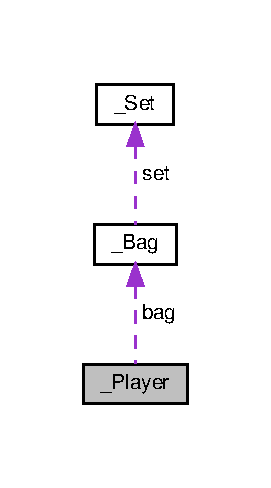
\includegraphics[width=130pt]{struct__Player__coll__graph}
\end{center}
\end{figure}
\subsection*{Data Fields}
\begin{DoxyCompactItemize}
\item 
\mbox{\Hypertarget{struct__Player_a60d635cd063816a9c1bd873f4868bb90}\label{struct__Player_a60d635cd063816a9c1bd873f4868bb90}} 
\hyperlink{types_8h_a845e604fb28f7e3d97549da3448149d3}{Id} \hyperlink{struct__Player_a60d635cd063816a9c1bd873f4868bb90}{id}
\begin{DoxyCompactList}\small\item\em defines id \end{DoxyCompactList}\item 
\mbox{\Hypertarget{struct__Player_ac89715f913cc607b75eb7236765c41f5}\label{struct__Player_ac89715f913cc607b75eb7236765c41f5}} 
char \hyperlink{struct__Player_ac89715f913cc607b75eb7236765c41f5}{name} \mbox{[}\hyperlink{types_8h_a92ed8507d1cd2331ad09275c5c4c1c89}{W\+O\+R\+D\+\_\+\+S\+I\+ZE}+1\mbox{]}
\begin{DoxyCompactList}\small\item\em defines string name \end{DoxyCompactList}\item 
\mbox{\Hypertarget{struct__Player_adbb6195d15b88f3f658e74274eff52d8}\label{struct__Player_adbb6195d15b88f3f658e74274eff52d8}} 
\hyperlink{types_8h_a845e604fb28f7e3d97549da3448149d3}{Id} \hyperlink{struct__Player_adbb6195d15b88f3f658e74274eff52d8}{location}
\begin{DoxyCompactList}\small\item\em defines id locatiom \end{DoxyCompactList}\item 
\mbox{\Hypertarget{struct__Player_a723e17ec37bbe34a7d61c1a8f5d5d0bd}\label{struct__Player_a723e17ec37bbe34a7d61c1a8f5d5d0bd}} 
\hyperlink{inventory_8h_a96eaad8b37d9b6e19ddc373ec38c751e}{Bag} $\ast$ \hyperlink{struct__Player_a723e17ec37bbe34a7d61c1a8f5d5d0bd}{bag}
\begin{DoxyCompactList}\small\item\em defines pointer to bag \end{DoxyCompactList}\end{DoxyCompactItemize}


\subsection{Detailed Description}
defines the structure of player 

The documentation for this struct was generated from the following file\+:\begin{DoxyCompactItemize}
\item 
\hyperlink{player_8c}{player.\+c}\end{DoxyCompactItemize}

\hypertarget{struct__Rules}{}\section{\+\_\+\+Rules Struct Reference}
\label{struct__Rules}\index{\+\_\+\+Rules@{\+\_\+\+Rules}}


defines the rules structure  




Collaboration diagram for \+\_\+\+Rules\+:
\nopagebreak
\begin{figure}[H]
\begin{center}
\leavevmode
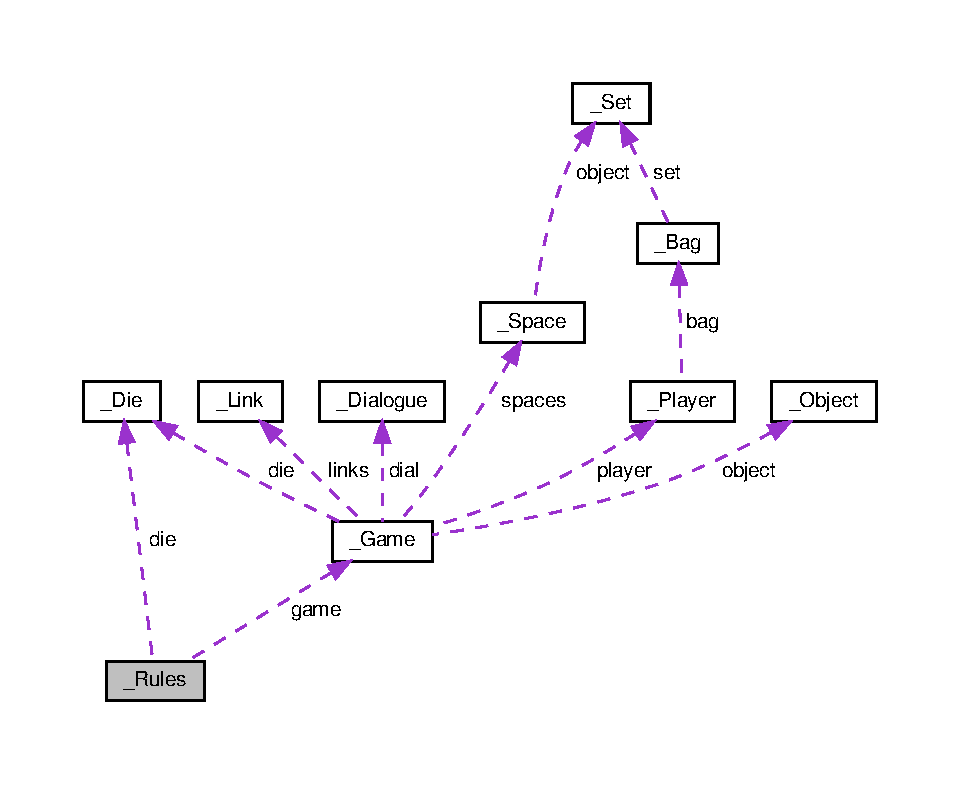
\includegraphics[width=350pt]{struct__Rules__coll__graph}
\end{center}
\end{figure}
\subsection*{Data Fields}
\begin{DoxyCompactItemize}
\item 
\mbox{\Hypertarget{struct__Rules_a9febb4df1e8e36c8340c9d6b206d2d3c}\label{struct__Rules_a9febb4df1e8e36c8340c9d6b206d2d3c}} 
\hyperlink{game__rules_8h_a7a04f8c7bfd4a66dd1aa598a1f6f9c6c}{Rule\+List} \hyperlink{struct__Rules_a9febb4df1e8e36c8340c9d6b206d2d3c}{rulelist}
\begin{DoxyCompactList}\small\item\em defines the variable rulelist \end{DoxyCompactList}\item 
\mbox{\Hypertarget{struct__Rules_abdbc2fc4222a97be384ddcc61425b6ec}\label{struct__Rules_abdbc2fc4222a97be384ddcc61425b6ec}} 
\hyperlink{die_8h_a892f0b0bf81d69a1f7a14ea238e36dd3}{Die} $\ast$ \hyperlink{struct__Rules_abdbc2fc4222a97be384ddcc61425b6ec}{die}
\begin{DoxyCompactList}\small\item\em defines the variable die \end{DoxyCompactList}\item 
\mbox{\Hypertarget{struct__Rules_a416c4fd5f34414b4cc3932d3bde207be}\label{struct__Rules_a416c4fd5f34414b4cc3932d3bde207be}} 
\hyperlink{game_8h_a57156d39c530aec3fba3a9dad8c2dc6a}{Game} $\ast$ \hyperlink{struct__Rules_a416c4fd5f34414b4cc3932d3bde207be}{game}
\begin{DoxyCompactList}\small\item\em defines the variable game \end{DoxyCompactList}\end{DoxyCompactItemize}


\subsection{Detailed Description}
defines the rules structure 

The documentation for this struct was generated from the following file\+:\begin{DoxyCompactItemize}
\item 
\hyperlink{game__rules_8c}{game\+\_\+rules.\+c}\end{DoxyCompactItemize}

\hypertarget{struct__Set}{\section{\+\_\+\+Set Struct Reference}
\label{struct__Set}\index{\+\_\+\+Set@{\+\_\+\+Set}}
}


Estructura del set.  


\subsection*{Public Attributes}
\begin{DoxyCompactItemize}
\item 
\hyperlink{types_8h_a845e604fb28f7e3d97549da3448149d3}{Id} \hyperlink{struct__Set_ade7a01e5a10383074adabe6bb75a1e24}{id} \mbox{[}\hyperlink{set_8h_a1cdef4472847c938fc165b7d2737c4e4}{M\+A\+X\+\_\+\+I\+D}\mbox{]}
\item 
int \hyperlink{struct__Set_a42aaa7654deed021016675f5008b15d2}{n\+Id}
\end{DoxyCompactItemize}


\subsection{Detailed Description}
Estructura del set. 

\subsection{Member Data Documentation}
\hypertarget{struct__Set_ade7a01e5a10383074adabe6bb75a1e24}{\index{\+\_\+\+Set@{\+\_\+\+Set}!id@{id}}
\index{id@{id}!\+\_\+\+Set@{\+\_\+\+Set}}
\subsubsection[{id}]{\setlength{\rightskip}{0pt plus 5cm}{\bf Id} \+\_\+\+Set\+::id\mbox{[}{\bf M\+A\+X\+\_\+\+I\+D}\mbox{]}}}\label{struct__Set_ade7a01e5a10383074adabe6bb75a1e24}
identificador del objeto \hypertarget{struct__Set_a42aaa7654deed021016675f5008b15d2}{\index{\+\_\+\+Set@{\+\_\+\+Set}!n\+Id@{n\+Id}}
\index{n\+Id@{n\+Id}!\+\_\+\+Set@{\+\_\+\+Set}}
\subsubsection[{n\+Id}]{\setlength{\rightskip}{0pt plus 5cm}int \+\_\+\+Set\+::n\+Id}}\label{struct__Set_a42aaa7654deed021016675f5008b15d2}
numero de ids 

The documentation for this struct was generated from the following file\+:\begin{DoxyCompactItemize}
\item 
src/\hyperlink{set_8c}{set.\+c}\end{DoxyCompactItemize}

\hypertarget{struct__Space}{}\section{\+\_\+\+Space Struct Reference}
\label{struct__Space}\index{\+\_\+\+Space@{\+\_\+\+Space}}


defines the structure of space  




Collaboration diagram for \+\_\+\+Space\+:
\nopagebreak
\begin{figure}[H]
\begin{center}
\leavevmode
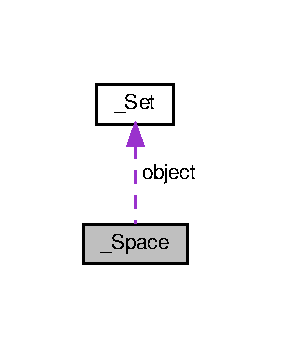
\includegraphics[width=135pt]{struct__Space__coll__graph}
\end{center}
\end{figure}
\subsection*{Data Fields}
\begin{DoxyCompactItemize}
\item 
\mbox{\Hypertarget{struct__Space_a70cb461deb9ac073e401b607339b567f}\label{struct__Space_a70cb461deb9ac073e401b607339b567f}} 
\hyperlink{types_8h_a845e604fb28f7e3d97549da3448149d3}{Id} \hyperlink{struct__Space_a70cb461deb9ac073e401b607339b567f}{id}
\begin{DoxyCompactList}\small\item\em defines id \end{DoxyCompactList}\item 
\mbox{\Hypertarget{struct__Space_aa1c9c994c2d16ecf3ef46138685fdfdc}\label{struct__Space_aa1c9c994c2d16ecf3ef46138685fdfdc}} 
char \hyperlink{struct__Space_aa1c9c994c2d16ecf3ef46138685fdfdc}{name} \mbox{[}\hyperlink{types_8h_a92ed8507d1cd2331ad09275c5c4c1c89}{W\+O\+R\+D\+\_\+\+S\+I\+ZE}+1\mbox{]}
\begin{DoxyCompactList}\small\item\em defines string name \end{DoxyCompactList}\item 
\mbox{\Hypertarget{struct__Space_ae5ebe53ce79514d7d2d93911e0159252}\label{struct__Space_ae5ebe53ce79514d7d2d93911e0159252}} 
\hyperlink{types_8h_a845e604fb28f7e3d97549da3448149d3}{Id} \hyperlink{struct__Space_ae5ebe53ce79514d7d2d93911e0159252}{north}
\begin{DoxyCompactList}\small\item\em defines id north \end{DoxyCompactList}\item 
\mbox{\Hypertarget{struct__Space_a646b68c22a0bbf1685033c96109d31d1}\label{struct__Space_a646b68c22a0bbf1685033c96109d31d1}} 
\hyperlink{types_8h_a845e604fb28f7e3d97549da3448149d3}{Id} \hyperlink{struct__Space_a646b68c22a0bbf1685033c96109d31d1}{south}
\begin{DoxyCompactList}\small\item\em defines id south \end{DoxyCompactList}\item 
\mbox{\Hypertarget{struct__Space_a41ce2bf33cf0c157b358221f094ee05b}\label{struct__Space_a41ce2bf33cf0c157b358221f094ee05b}} 
\hyperlink{types_8h_a845e604fb28f7e3d97549da3448149d3}{Id} \hyperlink{struct__Space_a41ce2bf33cf0c157b358221f094ee05b}{east}
\begin{DoxyCompactList}\small\item\em defines id east \end{DoxyCompactList}\item 
\mbox{\Hypertarget{struct__Space_a20c1d259e93b44e24ba82982e142eb9b}\label{struct__Space_a20c1d259e93b44e24ba82982e142eb9b}} 
\hyperlink{types_8h_a845e604fb28f7e3d97549da3448149d3}{Id} \hyperlink{struct__Space_a20c1d259e93b44e24ba82982e142eb9b}{west}
\begin{DoxyCompactList}\small\item\em defines id west \end{DoxyCompactList}\item 
\mbox{\Hypertarget{struct__Space_af55fb96d4a4fc2028959c409c8fadaf0}\label{struct__Space_af55fb96d4a4fc2028959c409c8fadaf0}} 
\hyperlink{set_8h_a6d3b7f7c92cbb4577ef3ef7ddbf93161}{Set} $\ast$ \hyperlink{struct__Space_af55fb96d4a4fc2028959c409c8fadaf0}{object}
\begin{DoxyCompactList}\small\item\em defines set of objects \end{DoxyCompactList}\item 
\mbox{\Hypertarget{struct__Space_ab77f924c8f24489481b08653abc2aea7}\label{struct__Space_ab77f924c8f24489481b08653abc2aea7}} 
char $\ast$ \hyperlink{struct__Space_ab77f924c8f24489481b08653abc2aea7}{gdesc1}
\begin{DoxyCompactList}\small\item\em defines gdesc1 \end{DoxyCompactList}\item 
\mbox{\Hypertarget{struct__Space_a0d4c7df1824c7d6d8bcdb01c39e963b3}\label{struct__Space_a0d4c7df1824c7d6d8bcdb01c39e963b3}} 
char $\ast$ \hyperlink{struct__Space_a0d4c7df1824c7d6d8bcdb01c39e963b3}{gdesc2}
\begin{DoxyCompactList}\small\item\em defines gdesc2 \end{DoxyCompactList}\item 
\mbox{\Hypertarget{struct__Space_a16ac903ceb338bd5730bab4e63ddbce4}\label{struct__Space_a16ac903ceb338bd5730bab4e63ddbce4}} 
char $\ast$ \hyperlink{struct__Space_a16ac903ceb338bd5730bab4e63ddbce4}{gdesc3}
\begin{DoxyCompactList}\small\item\em defines gdesc3 \end{DoxyCompactList}\item 
\mbox{\Hypertarget{struct__Space_a41a1dbfab1d88b732db50d7335c2f328}\label{struct__Space_a41a1dbfab1d88b732db50d7335c2f328}} 
char \hyperlink{struct__Space_a41a1dbfab1d88b732db50d7335c2f328}{description} \mbox{[}\hyperlink{types_8h_a92ed8507d1cd2331ad09275c5c4c1c89}{W\+O\+R\+D\+\_\+\+S\+I\+ZE}+1\mbox{]}
\begin{DoxyCompactList}\small\item\em defines description \end{DoxyCompactList}\end{DoxyCompactItemize}


\subsection{Detailed Description}
defines the structure of space 

The documentation for this struct was generated from the following file\+:\begin{DoxyCompactItemize}
\item 
\hyperlink{space_8c}{space.\+c}\end{DoxyCompactItemize}

\chapter{File Documentation}
\hypertarget{command_8c}{}\section{command.\+c File Reference}
\label{command_8c}\index{command.\+c@{command.\+c}}


It implements the command interpreter.  


{\ttfamily \#include $<$stdio.\+h$>$}\newline
{\ttfamily \#include $<$strings.\+h$>$}\newline
{\ttfamily \#include \char`\"{}command.\+h\char`\"{}}\newline
Include dependency graph for command.\+c\+:
\nopagebreak
\begin{figure}[H]
\begin{center}
\leavevmode
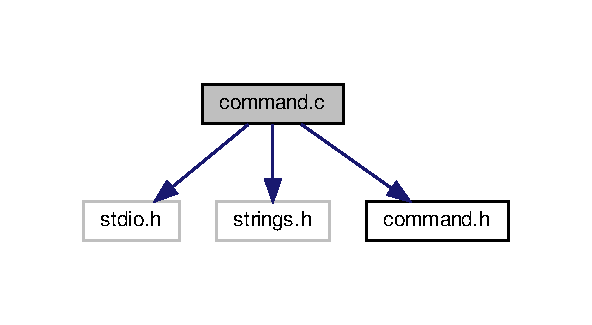
\includegraphics[width=284pt]{command_8c__incl}
\end{center}
\end{figure}
\subsection*{Macros}
\begin{DoxyCompactItemize}
\item 
\mbox{\Hypertarget{command_8c_a2b1bd24d2eddf8081d8c541e4cc4fd4b}\label{command_8c_a2b1bd24d2eddf8081d8c541e4cc4fd4b}} 
\#define \hyperlink{command_8c_a2b1bd24d2eddf8081d8c541e4cc4fd4b}{C\+M\+D\+\_\+\+L\+E\+N\+G\+HT}~30
\begin{DoxyCompactList}\small\item\em It defines the lenght of cmd. \end{DoxyCompactList}\item 
\mbox{\Hypertarget{command_8c_ae180fe89f0ae48ce5c80ffaa18de9271}\label{command_8c_ae180fe89f0ae48ce5c80ffaa18de9271}} 
\#define \hyperlink{command_8c_ae180fe89f0ae48ce5c80ffaa18de9271}{N\+\_\+\+C\+MD}~19
\begin{DoxyCompactList}\small\item\em It defines the number of cmd. \end{DoxyCompactList}\end{DoxyCompactItemize}
\subsection*{Functions}
\begin{DoxyCompactItemize}
\item 
\hyperlink{command_8h_a0473597db8c45c0289b6b8e2f8abbe32}{T\+\_\+\+Command} \hyperlink{command_8c_afe107f7479f6f9f3eab2078508fdfd55}{get\+\_\+user\+\_\+input} ()
\begin{DoxyCompactList}\small\item\em it gives the indication of what to do when receiving a command \end{DoxyCompactList}\end{DoxyCompactItemize}
\subsection*{Variables}
\begin{DoxyCompactItemize}
\item 
\mbox{\Hypertarget{command_8c_aa491d83d4e2f55a3074e418318a8d0fe}\label{command_8c_aa491d83d4e2f55a3074e418318a8d0fe}} 
char $\ast$ \hyperlink{command_8c_aa491d83d4e2f55a3074e418318a8d0fe}{cmd\+\_\+to\+\_\+str} \mbox{[}\hyperlink{command_8c_ae180fe89f0ae48ce5c80ffaa18de9271}{N\+\_\+\+C\+MD}\mbox{]} = \{\char`\"{}No command\char`\"{}, \char`\"{}Unknown\char`\"{}, \char`\"{}Exit\char`\"{}, \char`\"{}Next\char`\"{}, \char`\"{}Back\char`\"{},\char`\"{}Pick\char`\"{},\char`\"{}Drop\char`\"{},\char`\"{}Roll\char`\"{},\char`\"{}Left\char`\"{},\char`\"{}Right\char`\"{}, \char`\"{}Up\char`\"{}, \char`\"{}Down\char`\"{}, \char`\"{}Move\char`\"{}, \char`\"{}Inspect\char`\"{}, \char`\"{}Open\char`\"{}, \char`\"{}Turnon\char`\"{},\char`\"{}Turnoff\char`\"{},\char`\"{}Save\char`\"{},\char`\"{}Load\char`\"{}\}
\begin{DoxyCompactList}\small\item\em it defines the commands that can be used in the game \end{DoxyCompactList}\item 
\mbox{\Hypertarget{command_8c_a6397d54c2691d7e8ffe9a8da5db5df58}\label{command_8c_a6397d54c2691d7e8ffe9a8da5db5df58}} 
char $\ast$ \hyperlink{command_8c_a6397d54c2691d7e8ffe9a8da5db5df58}{short\+\_\+cmd\+\_\+to\+\_\+str} \mbox{[}\hyperlink{command_8c_ae180fe89f0ae48ce5c80ffaa18de9271}{N\+\_\+\+C\+MD}\mbox{]} = \{\char`\"{}\char`\"{},\char`\"{}\char`\"{},\char`\"{}e\char`\"{},\char`\"{}n\char`\"{},\char`\"{}b\char`\"{},\char`\"{}p\char`\"{},\char`\"{}d\char`\"{},\char`\"{}rl\char`\"{},\char`\"{}l\char`\"{},\char`\"{}r\char`\"{},\char`\"{}u\char`\"{},\char`\"{}dw\char`\"{},\char`\"{}m\char`\"{},\char`\"{}i\char`\"{},\char`\"{}o\char`\"{},\char`\"{}to\char`\"{},\char`\"{}tf\char`\"{},\char`\"{}s\char`\"{},\char`\"{}ld\char`\"{}\}
\begin{DoxyCompactList}\small\item\em it defines the commands that can be used in the game \end{DoxyCompactList}\end{DoxyCompactItemize}


\subsection{Detailed Description}
It implements the command interpreter. 

It implements module of link, that joints the different spaces.

\begin{DoxyAuthor}{Author}
\end{DoxyAuthor}
\begin{DoxyVersion}{Version}
3.\+0 
\end{DoxyVersion}
\begin{DoxyDate}{Date}
04-\/02-\/2019 
\end{DoxyDate}
\begin{DoxyCopyright}{Copyright}
G\+NU Public License
\end{DoxyCopyright}
\begin{DoxyAuthor}{Author}
\end{DoxyAuthor}
\begin{DoxyVersion}{Version}
1.\+0 
\end{DoxyVersion}
\begin{DoxyDate}{Date}
04-\/02-\/2019 
\end{DoxyDate}
\begin{DoxyCopyright}{Copyright}
G\+NU Public License 
\end{DoxyCopyright}


\subsection{Function Documentation}
\mbox{\Hypertarget{command_8c_afe107f7479f6f9f3eab2078508fdfd55}\label{command_8c_afe107f7479f6f9f3eab2078508fdfd55}} 
\index{command.\+c@{command.\+c}!get\+\_\+user\+\_\+input@{get\+\_\+user\+\_\+input}}
\index{get\+\_\+user\+\_\+input@{get\+\_\+user\+\_\+input}!command.\+c@{command.\+c}}
\subsubsection{\texorpdfstring{get\+\_\+user\+\_\+input()}{get\_user\_input()}}
{\footnotesize\ttfamily \hyperlink{command_8h_a0473597db8c45c0289b6b8e2f8abbe32}{T\+\_\+\+Command} get\+\_\+user\+\_\+input (\begin{DoxyParamCaption}{ }\end{DoxyParamCaption})}



it gives the indication of what to do when receiving a command 

it gets the input of user 

\hypertarget{command_8h}{}\section{command.\+h File Reference}
\label{command_8h}\index{command.\+h@{command.\+h}}


It defines the module of command.  


This graph shows which files directly or indirectly include this file\+:
\nopagebreak
\begin{figure}[H]
\begin{center}
\leavevmode
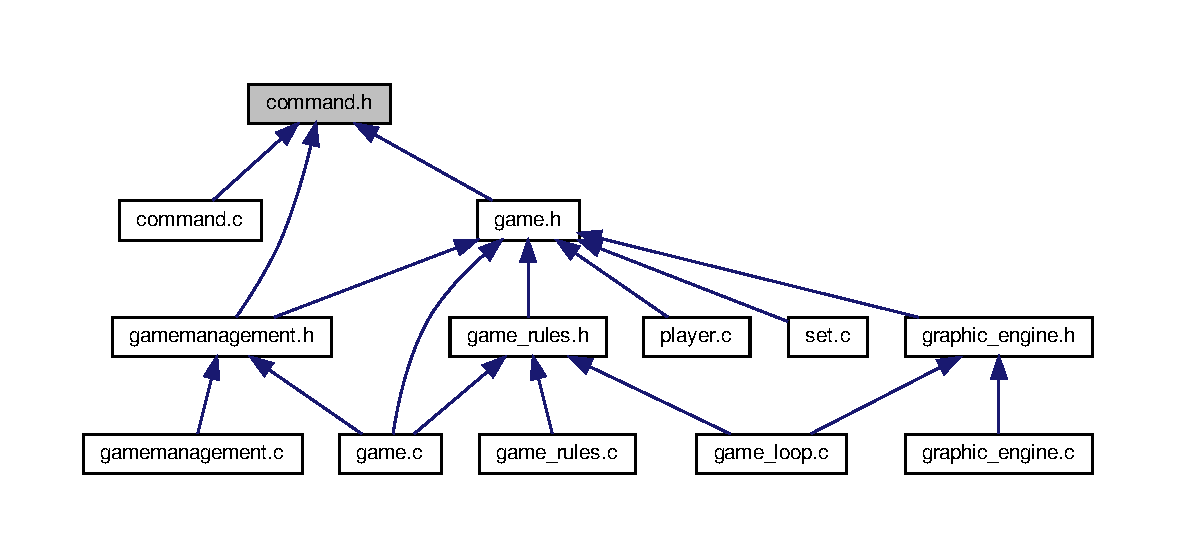
\includegraphics[width=350pt]{command_8h__dep__incl}
\end{center}
\end{figure}
\subsection*{Typedefs}
\begin{DoxyCompactItemize}
\item 
\mbox{\Hypertarget{command_8h_a0473597db8c45c0289b6b8e2f8abbe32}\label{command_8h_a0473597db8c45c0289b6b8e2f8abbe32}} 
typedef enum \hyperlink{command_8h_ace19ba2296a74e4aef53304e0934c50c}{enum\+\_\+\+Command} \hyperlink{command_8h_a0473597db8c45c0289b6b8e2f8abbe32}{T\+\_\+\+Command}
\begin{DoxyCompactList}\small\item\em It defines the header of command. \end{DoxyCompactList}\end{DoxyCompactItemize}
\subsection*{Enumerations}
\begin{DoxyCompactItemize}
\item 
\mbox{\Hypertarget{command_8h_ace19ba2296a74e4aef53304e0934c50c}\label{command_8h_ace19ba2296a74e4aef53304e0934c50c}} 
enum \hyperlink{command_8h_ace19ba2296a74e4aef53304e0934c50c}{enum\+\_\+\+Command} \{ \newline
{\bfseries N\+O\+\_\+\+C\+MD} = -\/1, 
{\bfseries U\+N\+K\+N\+O\+WN}, 
{\bfseries E\+X\+IT}, 
{\bfseries N\+E\+XT}, 
\newline
{\bfseries B\+A\+CK}, 
{\bfseries P\+I\+CK}, 
{\bfseries D\+R\+OP}, 
{\bfseries R\+O\+LL}
 \}\begin{DoxyCompactList}\small\item\em It defines the header of command. \end{DoxyCompactList}
\end{DoxyCompactItemize}
\subsection*{Functions}
\begin{DoxyCompactItemize}
\item 
\hyperlink{command_8h_a0473597db8c45c0289b6b8e2f8abbe32}{T\+\_\+\+Command} \hyperlink{command_8h_afe107f7479f6f9f3eab2078508fdfd55}{get\+\_\+user\+\_\+input} ()
\begin{DoxyCompactList}\small\item\em it gets the input of user \end{DoxyCompactList}\end{DoxyCompactItemize}


\subsection{Detailed Description}
It defines the module of command. 

\begin{DoxyAuthor}{Author}
\end{DoxyAuthor}
\begin{DoxyVersion}{Version}
2.\+0 
\end{DoxyVersion}
\begin{DoxyDate}{Date}
04-\/02-\/2019 
\end{DoxyDate}
\begin{DoxyCopyright}{Copyright}
G\+NU Public License 
\end{DoxyCopyright}


\subsection{Function Documentation}
\mbox{\Hypertarget{command_8h_afe107f7479f6f9f3eab2078508fdfd55}\label{command_8h_afe107f7479f6f9f3eab2078508fdfd55}} 
\index{command.\+h@{command.\+h}!get\+\_\+user\+\_\+input@{get\+\_\+user\+\_\+input}}
\index{get\+\_\+user\+\_\+input@{get\+\_\+user\+\_\+input}!command.\+h@{command.\+h}}
\subsubsection{\texorpdfstring{get\+\_\+user\+\_\+input()}{get\_user\_input()}}
{\footnotesize\ttfamily \hyperlink{command_8h_a0473597db8c45c0289b6b8e2f8abbe32}{T\+\_\+\+Command} get\+\_\+user\+\_\+input (\begin{DoxyParamCaption}{ }\end{DoxyParamCaption})}



it gets the input of user 

it gets the input of user 

\hypertarget{die_8c}{}\section{die.\+c File Reference}
\label{die_8c}\index{die.\+c@{die.\+c}}


It defines the module of die to obtain a number to go forware in the game.  


{\ttfamily \#include $<$stdio.\+h$>$}\newline
{\ttfamily \#include $<$stdlib.\+h$>$}\newline
{\ttfamily \#include $<$string.\+h$>$}\newline
{\ttfamily \#include $<$time.\+h$>$}\newline
{\ttfamily \#include \char`\"{}die.\+h\char`\"{}}\newline
Include dependency graph for die.\+c\+:
\nopagebreak
\begin{figure}[H]
\begin{center}
\leavevmode
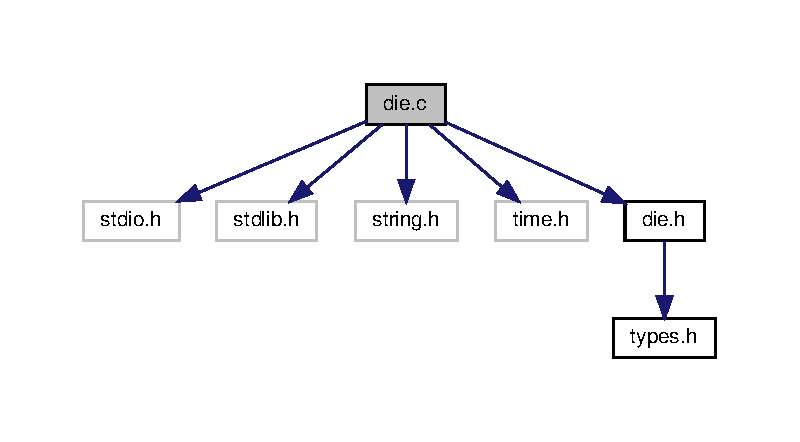
\includegraphics[width=350pt]{die_8c__incl}
\end{center}
\end{figure}
\subsection*{Data Structures}
\begin{DoxyCompactItemize}
\item 
struct \hyperlink{struct__Die}{\+\_\+\+Die}
\begin{DoxyCompactList}\small\item\em defines structure of die \end{DoxyCompactList}\end{DoxyCompactItemize}
\subsection*{Functions}
\begin{DoxyCompactItemize}
\item 
\hyperlink{die_8h_a892f0b0bf81d69a1f7a14ea238e36dd3}{Die} $\ast$ \hyperlink{die_8c_a413bced882cd5cadbb1d8feaf367ed3f}{die\+\_\+create} (\hyperlink{types_8h_a845e604fb28f7e3d97549da3448149d3}{Id} id)
\begin{DoxyCompactList}\small\item\em create a Die \end{DoxyCompactList}\item 
void \hyperlink{die_8c_a0155d7ec003966bace47f3e032a368e8}{die\+\_\+destroy} (\hyperlink{die_8h_a892f0b0bf81d69a1f7a14ea238e36dd3}{Die} $\ast$die)
\begin{DoxyCompactList}\small\item\em destroy a Die \end{DoxyCompactList}\item 
int \hyperlink{die_8c_a06289514edbedf660c4b043f78e859fc}{die\+\_\+roll} (\hyperlink{die_8h_a892f0b0bf81d69a1f7a14ea238e36dd3}{Die} $\ast$die)
\begin{DoxyCompactList}\small\item\em roll a Die \end{DoxyCompactList}\item 
int \hyperlink{die_8c_a2dbbc4fa2cb5dca61e2f86dbfc66ff4d}{die\+\_\+get\+\_\+value} (\hyperlink{die_8h_a892f0b0bf81d69a1f7a14ea238e36dd3}{Die} $\ast$die)
\begin{DoxyCompactList}\small\item\em get value of die \end{DoxyCompactList}\end{DoxyCompactItemize}


\subsection{Detailed Description}
It defines the module of die to obtain a number to go forware in the game. 

\begin{DoxyAuthor}{Author}
\end{DoxyAuthor}
\begin{DoxyVersion}{Version}
1.\+0 
\end{DoxyVersion}
\begin{DoxyDate}{Date}
28-\/02-\/2019 
\end{DoxyDate}
\begin{DoxyCopyright}{Copyright}
G\+NU Public License 
\end{DoxyCopyright}


\subsection{Function Documentation}
\mbox{\Hypertarget{die_8c_a413bced882cd5cadbb1d8feaf367ed3f}\label{die_8c_a413bced882cd5cadbb1d8feaf367ed3f}} 
\index{die.\+c@{die.\+c}!die\+\_\+create@{die\+\_\+create}}
\index{die\+\_\+create@{die\+\_\+create}!die.\+c@{die.\+c}}
\subsubsection{\texorpdfstring{die\+\_\+create()}{die\_create()}}
{\footnotesize\ttfamily \hyperlink{die_8h_a892f0b0bf81d69a1f7a14ea238e36dd3}{Die}$\ast$ die\+\_\+create (\begin{DoxyParamCaption}\item[{\hyperlink{types_8h_a845e604fb28f7e3d97549da3448149d3}{Id}}]{id }\end{DoxyParamCaption})}



create a Die 


\begin{DoxyParams}{Parameters}
{\em id} & \\
\hline
\end{DoxyParams}
\begin{DoxyReturn}{Returns}
die n or in case of error it returns E\+R\+R\+OR 
\end{DoxyReturn}
\mbox{\Hypertarget{die_8c_a0155d7ec003966bace47f3e032a368e8}\label{die_8c_a0155d7ec003966bace47f3e032a368e8}} 
\index{die.\+c@{die.\+c}!die\+\_\+destroy@{die\+\_\+destroy}}
\index{die\+\_\+destroy@{die\+\_\+destroy}!die.\+c@{die.\+c}}
\subsubsection{\texorpdfstring{die\+\_\+destroy()}{die\_destroy()}}
{\footnotesize\ttfamily void die\+\_\+destroy (\begin{DoxyParamCaption}\item[{\hyperlink{die_8h_a892f0b0bf81d69a1f7a14ea238e36dd3}{Die} $\ast$}]{die }\end{DoxyParamCaption})}



destroy a Die 


\begin{DoxyParams}{Parameters}
{\em die} & \\
\hline
\end{DoxyParams}
\begin{DoxyReturn}{Returns}
void 
\end{DoxyReturn}
\mbox{\Hypertarget{die_8c_a2dbbc4fa2cb5dca61e2f86dbfc66ff4d}\label{die_8c_a2dbbc4fa2cb5dca61e2f86dbfc66ff4d}} 
\index{die.\+c@{die.\+c}!die\+\_\+get\+\_\+value@{die\+\_\+get\+\_\+value}}
\index{die\+\_\+get\+\_\+value@{die\+\_\+get\+\_\+value}!die.\+c@{die.\+c}}
\subsubsection{\texorpdfstring{die\+\_\+get\+\_\+value()}{die\_get\_value()}}
{\footnotesize\ttfamily int die\+\_\+get\+\_\+value (\begin{DoxyParamCaption}\item[{\hyperlink{die_8h_a892f0b0bf81d69a1f7a14ea238e36dd3}{Die} $\ast$}]{die }\end{DoxyParamCaption})}



get value of die 


\begin{DoxyParams}{Parameters}
{\em die} & \\
\hline
\end{DoxyParams}
\begin{DoxyReturn}{Returns}
int die number,in case of error -\/1 
\end{DoxyReturn}
\mbox{\Hypertarget{die_8c_a06289514edbedf660c4b043f78e859fc}\label{die_8c_a06289514edbedf660c4b043f78e859fc}} 
\index{die.\+c@{die.\+c}!die\+\_\+roll@{die\+\_\+roll}}
\index{die\+\_\+roll@{die\+\_\+roll}!die.\+c@{die.\+c}}
\subsubsection{\texorpdfstring{die\+\_\+roll()}{die\_roll()}}
{\footnotesize\ttfamily int die\+\_\+roll (\begin{DoxyParamCaption}\item[{\hyperlink{die_8h_a892f0b0bf81d69a1f7a14ea238e36dd3}{Die} $\ast$}]{die }\end{DoxyParamCaption})}



roll a Die 


\begin{DoxyParams}{Parameters}
{\em die} & \\
\hline
\end{DoxyParams}
\begin{DoxyReturn}{Returns}
int die number,in case of error -\/1 
\end{DoxyReturn}


\hypertarget{die_8h}{\section{include/die.h File Reference}
\label{die_8h}\index{include/die.\+h@{include/die.\+h}}
}


It implements the die interpreter.  


{\ttfamily \#include \char`\"{}../include/types.\+h\char`\"{}}\\*
Include dependency graph for die.\+h\+:
\nopagebreak
\begin{figure}[H]
\begin{center}
\leavevmode
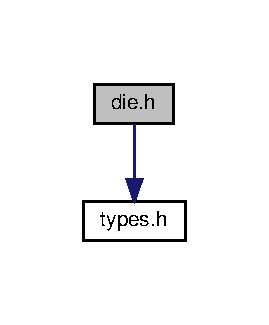
\includegraphics[width=172pt]{die_8h__incl}
\end{center}
\end{figure}
This graph shows which files directly or indirectly include this file\+:
\nopagebreak
\begin{figure}[H]
\begin{center}
\leavevmode
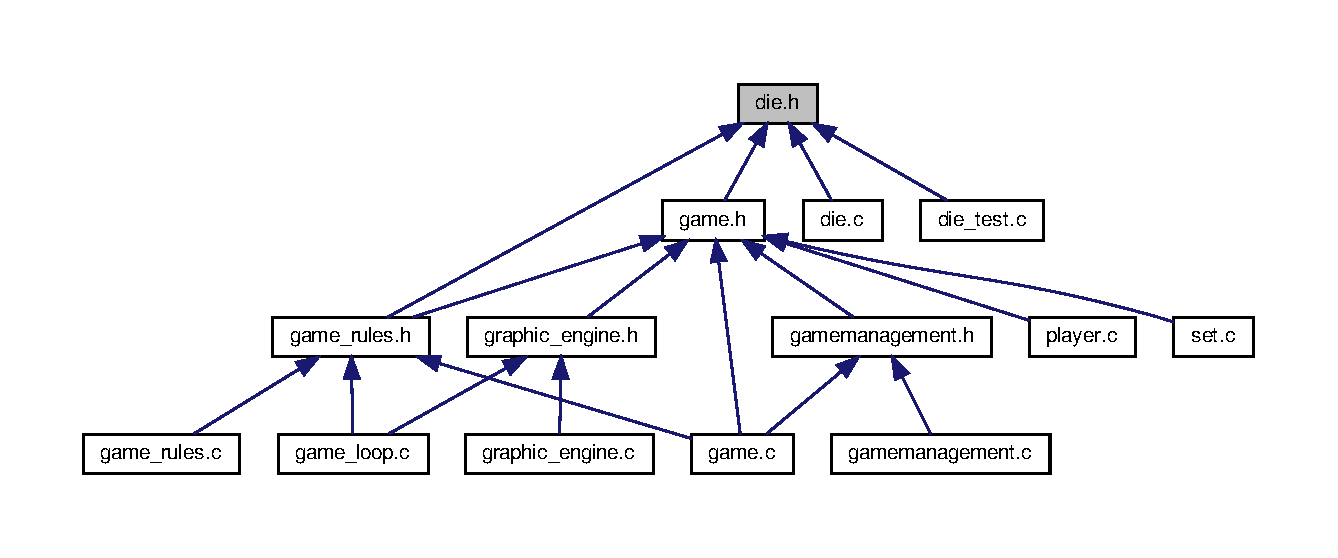
\includegraphics[width=350pt]{die_8h__dep__incl}
\end{center}
\end{figure}
\subsection*{Typedefs}
\begin{DoxyCompactItemize}
\item 
\hypertarget{die_8h_a892f0b0bf81d69a1f7a14ea238e36dd3}{typedef struct \hyperlink{struct__Die}{\+\_\+\+Die} \hyperlink{die_8h_a892f0b0bf81d69a1f7a14ea238e36dd3}{Die}}\label{die_8h_a892f0b0bf81d69a1f7a14ea238e36dd3}

\begin{DoxyCompactList}\small\item\em Estructura del dado. \end{DoxyCompactList}\end{DoxyCompactItemize}
\subsection*{Functions}
\begin{DoxyCompactItemize}
\item 
\hyperlink{die_8h_a892f0b0bf81d69a1f7a14ea238e36dd3}{Die} $\ast$ \hyperlink{die_8h_a413bced882cd5cadbb1d8feaf367ed3f}{die\+\_\+create} (\hyperlink{types_8h_a845e604fb28f7e3d97549da3448149d3}{Id} id)
\begin{DoxyCompactList}\small\item\em Funcion encargada de reservar memoria para el dado. \end{DoxyCompactList}\item 
\hyperlink{types_8h_a32c27cc471df37f4fc818d65de0a56c4}{S\+T\+A\+T\+U\+S} \hyperlink{die_8h_a2115999335e58f733d846be485cfb783}{die\+\_\+destroy} (\hyperlink{die_8h_a892f0b0bf81d69a1f7a14ea238e36dd3}{Die} $\ast$die)
\begin{DoxyCompactList}\small\item\em Funcion encargada de liberar la memoria reservada para el dado. \end{DoxyCompactList}\item 
\hyperlink{types_8h_a845e604fb28f7e3d97549da3448149d3}{Id} \hyperlink{die_8h_a57c9a2627bb3a1ca04fe55d72bd6a5ea}{die\+\_\+get\+\_\+id} (\hyperlink{die_8h_a892f0b0bf81d69a1f7a14ea238e36dd3}{Die} $\ast$die)
\begin{DoxyCompactList}\small\item\em Funcion encargada de obtener el id del dado. \end{DoxyCompactList}\item 
size\+\_\+t \hyperlink{die_8h_a1f2178342235c18c32c54ccd849c3ffe}{die\+\_\+get\+\_\+size} ()
\begin{DoxyCompactList}\small\item\em Funcion encargada de devolver el tamaño en memoria del dado. \end{DoxyCompactList}\item 
\hyperlink{types_8h_a32c27cc471df37f4fc818d65de0a56c4}{S\+T\+A\+T\+U\+S} \hyperlink{die_8h_a9a228775f79979e28bb3b4eea507f3d6}{die\+\_\+roll} (\hyperlink{die_8h_a892f0b0bf81d69a1f7a14ea238e36dd3}{Die} $\ast$dado, int sup, int inf)
\begin{DoxyCompactList}\small\item\em Funcion para lanzar el dado. \end{DoxyCompactList}\item 
\hyperlink{types_8h_a32c27cc471df37f4fc818d65de0a56c4}{S\+T\+A\+T\+U\+S} \hyperlink{die_8h_a6ab2e5a9dcbd7ba3bf9ac6ebb183ac97}{die\+\_\+print} (\hyperlink{die_8h_a892f0b0bf81d69a1f7a14ea238e36dd3}{Die} $\ast$die)
\begin{DoxyCompactList}\small\item\em Funcion encargada de darnos toda la informacion de un dado. \end{DoxyCompactList}\item 
int \hyperlink{die_8h_afef04ed0f9c6f21afcd1defa1e235b4e}{die\+\_\+get\+\_\+last\+Value} (\hyperlink{die_8h_a892f0b0bf81d69a1f7a14ea238e36dd3}{Die} $\ast$die)
\begin{DoxyCompactList}\small\item\em Funcion encargada de darnos el ultimo valor del dado. \end{DoxyCompactList}\end{DoxyCompactItemize}


\subsection{Detailed Description}
It implements the die interpreter. 

\begin{DoxyAuthor}{Author}
Julia Simon 
\end{DoxyAuthor}
\begin{DoxyVersion}{Version}
1.\+0 
\end{DoxyVersion}
\begin{DoxyDate}{Date}
20/02/2018 
\end{DoxyDate}


\subsection{Function Documentation}
\hypertarget{die_8h_a413bced882cd5cadbb1d8feaf367ed3f}{\index{die.\+h@{die.\+h}!die\+\_\+create@{die\+\_\+create}}
\index{die\+\_\+create@{die\+\_\+create}!die.\+h@{die.\+h}}
\subsubsection[{die\+\_\+create}]{\setlength{\rightskip}{0pt plus 5cm}{\bf Die}$\ast$ die\+\_\+create (
\begin{DoxyParamCaption}
\item[{{\bf Id}}]{id}
\end{DoxyParamCaption}
)}}\label{die_8h_a413bced882cd5cadbb1d8feaf367ed3f}


Funcion encargada de reservar memoria para el dado. 

\begin{DoxyAuthor}{Author}
Julia Simon 
\end{DoxyAuthor}

\begin{DoxyParams}{Parameters}
{\em Id} & id del dado que se va a crear \\
\hline
\end{DoxyParams}
\begin{DoxyReturn}{Returns}
dado que se ha creado 
\end{DoxyReturn}
\hypertarget{die_8h_a2115999335e58f733d846be485cfb783}{\index{die.\+h@{die.\+h}!die\+\_\+destroy@{die\+\_\+destroy}}
\index{die\+\_\+destroy@{die\+\_\+destroy}!die.\+h@{die.\+h}}
\subsubsection[{die\+\_\+destroy}]{\setlength{\rightskip}{0pt plus 5cm}{\bf S\+T\+A\+T\+U\+S} die\+\_\+destroy (
\begin{DoxyParamCaption}
\item[{{\bf Die} $\ast$}]{die}
\end{DoxyParamCaption}
)}}\label{die_8h_a2115999335e58f733d846be485cfb783}


Funcion encargada de liberar la memoria reservada para el dado. 

\begin{DoxyAuthor}{Author}
Julia Simon 
\end{DoxyAuthor}

\begin{DoxyParams}{Parameters}
{\em die} & dado que se quiere liberar \\
\hline
\end{DoxyParams}
\begin{DoxyReturn}{Returns}
O\+K si se ha liberado la memoria correctamente y E\+R\+R\+O\+R en caso de error 
\end{DoxyReturn}
\hypertarget{die_8h_a57c9a2627bb3a1ca04fe55d72bd6a5ea}{\index{die.\+h@{die.\+h}!die\+\_\+get\+\_\+id@{die\+\_\+get\+\_\+id}}
\index{die\+\_\+get\+\_\+id@{die\+\_\+get\+\_\+id}!die.\+h@{die.\+h}}
\subsubsection[{die\+\_\+get\+\_\+id}]{\setlength{\rightskip}{0pt plus 5cm}{\bf Id} die\+\_\+get\+\_\+id (
\begin{DoxyParamCaption}
\item[{{\bf Die} $\ast$}]{die}
\end{DoxyParamCaption}
)}}\label{die_8h_a57c9a2627bb3a1ca04fe55d72bd6a5ea}


Funcion encargada de obtener el id del dado. 

\begin{DoxyAuthor}{Author}
Julia Simon 
\end{DoxyAuthor}

\begin{DoxyParams}{Parameters}
{\em die} & dado del que se quiere saber el id \\
\hline
\end{DoxyParams}
\begin{DoxyReturn}{Returns}
id del dado 
\end{DoxyReturn}
\hypertarget{die_8h_afef04ed0f9c6f21afcd1defa1e235b4e}{\index{die.\+h@{die.\+h}!die\+\_\+get\+\_\+last\+Value@{die\+\_\+get\+\_\+last\+Value}}
\index{die\+\_\+get\+\_\+last\+Value@{die\+\_\+get\+\_\+last\+Value}!die.\+h@{die.\+h}}
\subsubsection[{die\+\_\+get\+\_\+last\+Value}]{\setlength{\rightskip}{0pt plus 5cm}int die\+\_\+get\+\_\+last\+Value (
\begin{DoxyParamCaption}
\item[{{\bf Die} $\ast$}]{die}
\end{DoxyParamCaption}
)}}\label{die_8h_afef04ed0f9c6f21afcd1defa1e235b4e}


Funcion encargada de darnos el ultimo valor del dado. 

\begin{DoxyAuthor}{Author}
Julia Simon 
\end{DoxyAuthor}

\begin{DoxyParams}{Parameters}
{\em die} & dado del que se quiere saber \\
\hline
\end{DoxyParams}
\begin{DoxyReturn}{Returns}
int con el numero correspondiente 
\end{DoxyReturn}
\hypertarget{die_8h_a1f2178342235c18c32c54ccd849c3ffe}{\index{die.\+h@{die.\+h}!die\+\_\+get\+\_\+size@{die\+\_\+get\+\_\+size}}
\index{die\+\_\+get\+\_\+size@{die\+\_\+get\+\_\+size}!die.\+h@{die.\+h}}
\subsubsection[{die\+\_\+get\+\_\+size}]{\setlength{\rightskip}{0pt plus 5cm}size\+\_\+t die\+\_\+get\+\_\+size (
\begin{DoxyParamCaption}
{}
\end{DoxyParamCaption}
)}}\label{die_8h_a1f2178342235c18c32c54ccd849c3ffe}


Funcion encargada de devolver el tamaño en memoria del dado. 

\begin{DoxyAuthor}{Author}
Julia Simon 
\end{DoxyAuthor}
\begin{DoxyReturn}{Returns}
tamaño del dado 
\end{DoxyReturn}
\hypertarget{die_8h_a6ab2e5a9dcbd7ba3bf9ac6ebb183ac97}{\index{die.\+h@{die.\+h}!die\+\_\+print@{die\+\_\+print}}
\index{die\+\_\+print@{die\+\_\+print}!die.\+h@{die.\+h}}
\subsubsection[{die\+\_\+print}]{\setlength{\rightskip}{0pt plus 5cm}{\bf S\+T\+A\+T\+U\+S} die\+\_\+print (
\begin{DoxyParamCaption}
\item[{{\bf Die} $\ast$}]{die}
\end{DoxyParamCaption}
)}}\label{die_8h_a6ab2e5a9dcbd7ba3bf9ac6ebb183ac97}


Funcion encargada de darnos toda la informacion de un dado. 

\begin{DoxyAuthor}{Author}
Julia Simon 
\end{DoxyAuthor}

\begin{DoxyParams}{Parameters}
{\em die} & dado del que se quiere saber toda la informacion \\
\hline
\end{DoxyParams}
\begin{DoxyReturn}{Returns}
O\+K si se ha impreso correctamente la informacion en el fichero, y E\+R\+R\+O\+R en caso contrario 
\end{DoxyReturn}
\hypertarget{die_8h_a9a228775f79979e28bb3b4eea507f3d6}{\index{die.\+h@{die.\+h}!die\+\_\+roll@{die\+\_\+roll}}
\index{die\+\_\+roll@{die\+\_\+roll}!die.\+h@{die.\+h}}
\subsubsection[{die\+\_\+roll}]{\setlength{\rightskip}{0pt plus 5cm}{\bf S\+T\+A\+T\+U\+S} die\+\_\+roll (
\begin{DoxyParamCaption}
\item[{{\bf Die} $\ast$}]{dado, }
\item[{int}]{sup, }
\item[{int}]{inf}
\end{DoxyParamCaption}
)}}\label{die_8h_a9a228775f79979e28bb3b4eea507f3d6}


Funcion para lanzar el dado. 

\begin{DoxyAuthor}{Author}
Julia Simon 
\end{DoxyAuthor}

\begin{DoxyParams}{Parameters}
{\em dado} & dado que queremos tirar \\
\hline
{\em sup} & numero máximo del dado \\
\hline
{\em inf} & numero mínimo del dado \\
\hline
\end{DoxyParams}
\begin{DoxyReturn}{Returns}
O\+K si no ha habido problemas, E\+R\+R\+O\+R en caso de fallo 
\end{DoxyReturn}

\hypertarget{die__test_8c}{}\section{die\+\_\+test.\+c File Reference}
\label{die__test_8c}\index{die\+\_\+test.\+c@{die\+\_\+test.\+c}}


It tests die module.  


{\ttfamily \#include $<$stdio.\+h$>$}\newline
{\ttfamily \#include $<$stdlib.\+h$>$}\newline
{\ttfamily \#include $<$string.\+h$>$}\newline
{\ttfamily \#include \char`\"{}die.\+h\char`\"{}}\newline
Include dependency graph for die\+\_\+test.\+c\+:
\nopagebreak
\begin{figure}[H]
\begin{center}
\leavevmode
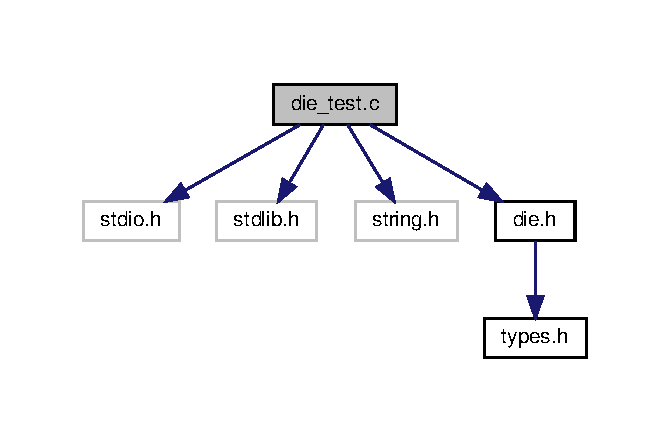
\includegraphics[width=322pt]{die__test_8c__incl}
\end{center}
\end{figure}
\subsection*{Functions}
\begin{DoxyCompactItemize}
\item 
int \hyperlink{die__test_8c_ae66f6b31b5ad750f1fe042a706a4e3d4}{main} ()
\begin{DoxyCompactList}\small\item\em main for testing \end{DoxyCompactList}\end{DoxyCompactItemize}


\subsection{Detailed Description}
It tests die module. 

It tests set module.

\begin{DoxyAuthor}{Author}
\end{DoxyAuthor}
\begin{DoxyVersion}{Version}
1.\+0 
\end{DoxyVersion}
\begin{DoxyDate}{Date}
28-\/02-\/2019 
\end{DoxyDate}
\begin{DoxyCopyright}{Copyright}
G\+NU Public License 
\end{DoxyCopyright}


\subsection{Function Documentation}
\mbox{\Hypertarget{die__test_8c_ae66f6b31b5ad750f1fe042a706a4e3d4}\label{die__test_8c_ae66f6b31b5ad750f1fe042a706a4e3d4}} 
\index{die\+\_\+test.\+c@{die\+\_\+test.\+c}!main@{main}}
\index{main@{main}!die\+\_\+test.\+c@{die\+\_\+test.\+c}}
\subsubsection{\texorpdfstring{main()}{main()}}
{\footnotesize\ttfamily int main (\begin{DoxyParamCaption}{ }\end{DoxyParamCaption})}



main for testing 

\begin{DoxyReturn}{Returns}
number 
\end{DoxyReturn}


\hypertarget{game_8c}{}\section{game.\+c File Reference}
\label{game_8c}\index{game.\+c@{game.\+c}}


It implements the game interface and all the associated callbacks for each command.  


{\ttfamily \#include $<$stdio.\+h$>$}\newline
{\ttfamily \#include $<$stdlib.\+h$>$}\newline
{\ttfamily \#include $<$string.\+h$>$}\newline
{\ttfamily \#include \char`\"{}game.\+h\char`\"{}}\newline
{\ttfamily \#include \char`\"{}gamemanagement.\+h\char`\"{}}\newline
{\ttfamily \#include \char`\"{}game\+\_\+rules.\+h\char`\"{}}\newline
Include dependency graph for game.\+c\+:
\nopagebreak
\begin{figure}[H]
\begin{center}
\leavevmode
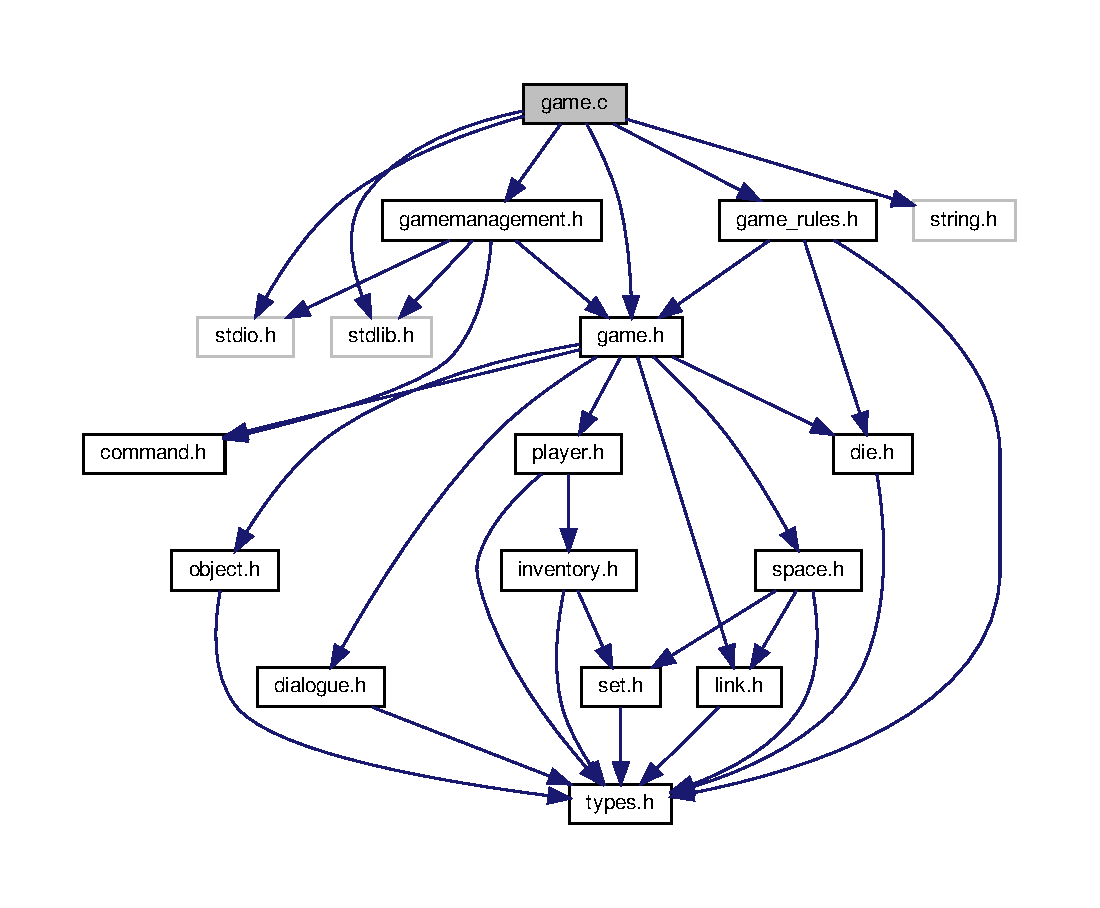
\includegraphics[width=350pt]{game_8c__incl}
\end{center}
\end{figure}
\subsection*{Data Structures}
\begin{DoxyCompactItemize}
\item 
struct \hyperlink{struct__Game}{\+\_\+\+Game}
\begin{DoxyCompactList}\small\item\em defines structure of game \end{DoxyCompactList}\end{DoxyCompactItemize}
\subsection*{Macros}
\begin{DoxyCompactItemize}
\item 
\mbox{\Hypertarget{game_8c_a8366e5ad74afbbea0cd0a414770c304a}\label{game_8c_a8366e5ad74afbbea0cd0a414770c304a}} 
\#define \hyperlink{game_8c_a8366e5ad74afbbea0cd0a414770c304a}{N\+\_\+\+C\+A\+L\+L\+B\+A\+CK}~18
\begin{DoxyCompactList}\small\item\em It defines the number of callbacks. \end{DoxyCompactList}\end{DoxyCompactItemize}
\subsection*{Typedefs}
\begin{DoxyCompactItemize}
\item 
typedef \hyperlink{types_8h_a32c27cc471df37f4fc818d65de0a56c4}{S\+T\+A\+T\+US}($\ast$ \hyperlink{game_8c_af87769c2b6d1d27086ca0ec91fcc4fea}{callback\+\_\+fn}) (\hyperlink{game_8h_a57156d39c530aec3fba3a9dad8c2dc6a}{Game} $\ast$game)
\end{DoxyCompactItemize}
\subsection*{Functions}
\begin{DoxyCompactItemize}
\item 
\hyperlink{types_8h_a32c27cc471df37f4fc818d65de0a56c4}{S\+T\+A\+T\+US} \hyperlink{game_8c_a39a8bb0b9b5eee8124f56573df4b77f8}{game\+\_\+callback\+\_\+unknown} (\hyperlink{game_8h_a57156d39c530aec3fba3a9dad8c2dc6a}{Game} $\ast$game)
\begin{DoxyCompactList}\small\item\em callback to unknown \end{DoxyCompactList}\item 
\hyperlink{types_8h_a32c27cc471df37f4fc818d65de0a56c4}{S\+T\+A\+T\+US} \hyperlink{game_8c_ab95080d04cabbb7a7aecc4e9d15ba955}{game\+\_\+callback\+\_\+exit} (\hyperlink{game_8h_a57156d39c530aec3fba3a9dad8c2dc6a}{Game} $\ast$game)
\begin{DoxyCompactList}\small\item\em callback to exit \end{DoxyCompactList}\item 
\hyperlink{types_8h_a32c27cc471df37f4fc818d65de0a56c4}{S\+T\+A\+T\+US} \hyperlink{game_8c_acc9f5c3994693938b92e3283f7f646a6}{game\+\_\+callback\+\_\+next} (\hyperlink{game_8h_a57156d39c530aec3fba3a9dad8c2dc6a}{Game} $\ast$game)
\begin{DoxyCompactList}\small\item\em callback to next \end{DoxyCompactList}\item 
\hyperlink{types_8h_a32c27cc471df37f4fc818d65de0a56c4}{S\+T\+A\+T\+US} \hyperlink{game_8c_af03ab41115b0e2fcdf5cd84a1b6cf159}{game\+\_\+callback\+\_\+back} (\hyperlink{game_8h_a57156d39c530aec3fba3a9dad8c2dc6a}{Game} $\ast$game)
\begin{DoxyCompactList}\small\item\em callback to back \end{DoxyCompactList}\item 
\hyperlink{types_8h_a32c27cc471df37f4fc818d65de0a56c4}{S\+T\+A\+T\+US} \hyperlink{game_8c_a344213bdec82cde227391d5bf806cf5b}{game\+\_\+callback\+\_\+\+Pick} (\hyperlink{game_8h_a57156d39c530aec3fba3a9dad8c2dc6a}{Game} $\ast$game)
\begin{DoxyCompactList}\small\item\em callback to pick \end{DoxyCompactList}\item 
\hyperlink{types_8h_a32c27cc471df37f4fc818d65de0a56c4}{S\+T\+A\+T\+US} \hyperlink{game_8c_a2efd1de83a4f88119767801bf0f45034}{game\+\_\+callback\+\_\+\+Drop} (\hyperlink{game_8h_a57156d39c530aec3fba3a9dad8c2dc6a}{Game} $\ast$game)
\begin{DoxyCompactList}\small\item\em callback to drop \end{DoxyCompactList}\item 
\hyperlink{types_8h_a32c27cc471df37f4fc818d65de0a56c4}{S\+T\+A\+T\+US} \hyperlink{game_8c_ab705d103d0a45cf9ea8a0f2b2be38eeb}{game\+\_\+callback\+\_\+\+Roll} (\hyperlink{game_8h_a57156d39c530aec3fba3a9dad8c2dc6a}{Game} $\ast$game)
\begin{DoxyCompactList}\small\item\em callback to roll \end{DoxyCompactList}\item 
\hyperlink{types_8h_a32c27cc471df37f4fc818d65de0a56c4}{S\+T\+A\+T\+US} \hyperlink{game_8c_a2d1163df1a6478c757e7a32cce9b8a5a}{game\+\_\+callback\+\_\+\+Left} (\hyperlink{game_8h_a57156d39c530aec3fba3a9dad8c2dc6a}{Game} $\ast$game)
\begin{DoxyCompactList}\small\item\em callback to left \end{DoxyCompactList}\item 
\hyperlink{types_8h_a32c27cc471df37f4fc818d65de0a56c4}{S\+T\+A\+T\+US} \hyperlink{game_8c_a43fbe9017f0ce39fce83dfd731818af3}{game\+\_\+callback\+\_\+\+Open} (\hyperlink{game_8h_a57156d39c530aec3fba3a9dad8c2dc6a}{Game} $\ast$game)
\begin{DoxyCompactList}\small\item\em callback to open \end{DoxyCompactList}\item 
\hyperlink{types_8h_a32c27cc471df37f4fc818d65de0a56c4}{S\+T\+A\+T\+US} \hyperlink{game_8c_ac84a4b62b3a7ccf6b0791a0890d73e76}{game\+\_\+callback\+\_\+\+Right} (\hyperlink{game_8h_a57156d39c530aec3fba3a9dad8c2dc6a}{Game} $\ast$game)
\begin{DoxyCompactList}\small\item\em callback to right \end{DoxyCompactList}\item 
\hyperlink{types_8h_a32c27cc471df37f4fc818d65de0a56c4}{S\+T\+A\+T\+US} \hyperlink{game_8c_ac3e4d9eb36cfba9bc4b1678ab5dccc60}{game\+\_\+callback\+\_\+\+Up} (\hyperlink{game_8h_a57156d39c530aec3fba3a9dad8c2dc6a}{Game} $\ast$game)
\begin{DoxyCompactList}\small\item\em callback to go up \end{DoxyCompactList}\item 
\hyperlink{types_8h_a32c27cc471df37f4fc818d65de0a56c4}{S\+T\+A\+T\+US} \hyperlink{game_8c_adc65490446fed7153765b182158c5288}{game\+\_\+callback\+\_\+\+Down} (\hyperlink{game_8h_a57156d39c530aec3fba3a9dad8c2dc6a}{Game} $\ast$game)
\begin{DoxyCompactList}\small\item\em callback to go down \end{DoxyCompactList}\item 
\hyperlink{types_8h_a32c27cc471df37f4fc818d65de0a56c4}{S\+T\+A\+T\+US} \hyperlink{game_8c_ac9415d81884bb07e8da882faa8d09148}{game\+\_\+callback\+\_\+\+Move} (\hyperlink{game_8h_a57156d39c530aec3fba3a9dad8c2dc6a}{Game} $\ast$game)
\begin{DoxyCompactList}\small\item\em callback to move \end{DoxyCompactList}\item 
\hyperlink{types_8h_a32c27cc471df37f4fc818d65de0a56c4}{S\+T\+A\+T\+US} \hyperlink{game_8c_a69ac5a72e1de17e0f0bfb26a1c589cc4}{game\+\_\+callback\+\_\+\+Inspect} (\hyperlink{game_8h_a57156d39c530aec3fba3a9dad8c2dc6a}{Game} $\ast$game)
\begin{DoxyCompactList}\small\item\em callback to inspect \end{DoxyCompactList}\item 
\hyperlink{types_8h_a32c27cc471df37f4fc818d65de0a56c4}{S\+T\+A\+T\+US} \hyperlink{game_8c_a15cf6b8e605b1605cebaf83e686c60a2}{game\+\_\+get\+\_\+callback\+\_\+status} (\hyperlink{game_8h_a57156d39c530aec3fba3a9dad8c2dc6a}{Game} $\ast$game)
\begin{DoxyCompactList}\small\item\em get callback \end{DoxyCompactList}\item 
\hyperlink{types_8h_a32c27cc471df37f4fc818d65de0a56c4}{S\+T\+A\+T\+US} \hyperlink{game_8c_ac2edd0091060ff9d13a9c356ac0edf2e}{game\+\_\+callback\+\_\+\+Turn\+On} (\hyperlink{game_8h_a57156d39c530aec3fba3a9dad8c2dc6a}{Game} $\ast$game)
\begin{DoxyCompactList}\small\item\em callback to turn ON \end{DoxyCompactList}\item 
\hyperlink{types_8h_a32c27cc471df37f4fc818d65de0a56c4}{S\+T\+A\+T\+US} \hyperlink{game_8c_a8ad700398578a58fabf4c38638a8cd84}{game\+\_\+callback\+\_\+\+Turn\+Off} (\hyperlink{game_8h_a57156d39c530aec3fba3a9dad8c2dc6a}{Game} $\ast$game)
\begin{DoxyCompactList}\small\item\em callback to turn O\+FF \end{DoxyCompactList}\item 
\hyperlink{types_8h_a32c27cc471df37f4fc818d65de0a56c4}{S\+T\+A\+T\+US} \hyperlink{game_8c_ae024c91a7ba2d02b47122f4a27640ecc}{game\+\_\+callback\+\_\+save} (\hyperlink{game_8h_a57156d39c530aec3fba3a9dad8c2dc6a}{Game} $\ast$game)
\begin{DoxyCompactList}\small\item\em callback to save game \end{DoxyCompactList}\item 
\hyperlink{types_8h_a32c27cc471df37f4fc818d65de0a56c4}{S\+T\+A\+T\+US} \hyperlink{game_8c_a46b1f9b02b168504ee1df1b3578fddac}{game\+\_\+callback\+\_\+load} (\hyperlink{game_8h_a57156d39c530aec3fba3a9dad8c2dc6a}{Game} $\ast$game)
\begin{DoxyCompactList}\small\item\em callback to load game \end{DoxyCompactList}\item 
\hyperlink{types_8h_a32c27cc471df37f4fc818d65de0a56c4}{S\+T\+A\+T\+US} \hyperlink{game_8c_a0d01072a28b01545d36240cb8bd9d4f8}{game\+\_\+load\+\_\+spaces} (\hyperlink{game_8h_a57156d39c530aec3fba3a9dad8c2dc6a}{Game} $\ast$game, char $\ast$filename)
\begin{DoxyCompactList}\small\item\em load spaces \end{DoxyCompactList}\item 
\hyperlink{types_8h_a845e604fb28f7e3d97549da3448149d3}{Id} \hyperlink{game_8c_ad2dfd865e2bd2c545a15d33f4d1cf3ae}{game\+\_\+get\+\_\+space\+\_\+id\+\_\+at} (\hyperlink{game_8h_a57156d39c530aec3fba3a9dad8c2dc6a}{Game} $\ast$game, int position)
\begin{DoxyCompactList}\small\item\em get spaces \end{DoxyCompactList}\item 
\hyperlink{types_8h_a32c27cc471df37f4fc818d65de0a56c4}{S\+T\+A\+T\+US} \hyperlink{game_8c_a492ca9fb594442dc43fc7d18a3820426}{game\+\_\+set\+\_\+player\+\_\+location} (\hyperlink{game_8h_a57156d39c530aec3fba3a9dad8c2dc6a}{Game} $\ast$game, \hyperlink{types_8h_a845e604fb28f7e3d97549da3448149d3}{Id} id)
\begin{DoxyCompactList}\small\item\em set player location \end{DoxyCompactList}\item 
\hyperlink{types_8h_a32c27cc471df37f4fc818d65de0a56c4}{S\+T\+A\+T\+US} \hyperlink{game_8c_a5d7aaff12ac7871d5d3d32697460086e}{game\+\_\+set\+\_\+object\+\_\+location} (\hyperlink{game_8h_a57156d39c530aec3fba3a9dad8c2dc6a}{Game} $\ast$game, \hyperlink{types_8h_a845e604fb28f7e3d97549da3448149d3}{Id} id, \hyperlink{types_8h_a845e604fb28f7e3d97549da3448149d3}{Id} loc)
\begin{DoxyCompactList}\small\item\em set object location \end{DoxyCompactList}\item 
\hyperlink{game_8h_a57156d39c530aec3fba3a9dad8c2dc6a}{Game} $\ast$ \hyperlink{game_8c_a1cdbe3f06b9bf49eb5e334a22ad3b2b9}{game\+\_\+create} ()
\begin{DoxyCompactList}\small\item\em create a game \end{DoxyCompactList}\item 
\hyperlink{types_8h_a32c27cc471df37f4fc818d65de0a56c4}{S\+T\+A\+T\+US} \hyperlink{game_8c_afc77f90739be0fd45b7f5616e543bfae}{game\+\_\+create\+\_\+from\+\_\+file} (\hyperlink{game_8h_a57156d39c530aec3fba3a9dad8c2dc6a}{Game} $\ast$game, char $\ast$filename)
\begin{DoxyCompactList}\small\item\em create file in game \end{DoxyCompactList}\item 
\hyperlink{types_8h_a32c27cc471df37f4fc818d65de0a56c4}{S\+T\+A\+T\+US} \hyperlink{game_8c_a0736924a1235c0e6fe9b6d91c2a12af8}{game\+\_\+destroy} (\hyperlink{game_8h_a57156d39c530aec3fba3a9dad8c2dc6a}{Game} $\ast$game)
\begin{DoxyCompactList}\small\item\em destroy game \end{DoxyCompactList}\item 
\hyperlink{types_8h_a32c27cc471df37f4fc818d65de0a56c4}{S\+T\+A\+T\+US} \hyperlink{game_8c_a48ef5745474ef224f39ed913c3a176e4}{game\+\_\+set\+\_\+objdsc} (\hyperlink{game_8h_a57156d39c530aec3fba3a9dad8c2dc6a}{Game} $\ast$game, char $\ast$objdsc)
\begin{DoxyCompactList}\small\item\em set objects of id i in the game \end{DoxyCompactList}\item 
char $\ast$ \hyperlink{game_8c_a83d23be85660b3a92d73268ba07638ea}{game\+\_\+get\+\_\+objdsc} (\hyperlink{game_8h_a57156d39c530aec3fba3a9dad8c2dc6a}{Game} $\ast$game)
\begin{DoxyCompactList}\small\item\em get the name of objects \end{DoxyCompactList}\item 
\hyperlink{types_8h_a32c27cc471df37f4fc818d65de0a56c4}{S\+T\+A\+T\+US} \hyperlink{game_8c_ada092ece1531e2c165bc7683e720f35b}{game\+\_\+set\+\_\+rule} (\hyperlink{game_8h_a57156d39c530aec3fba3a9dad8c2dc6a}{Game} $\ast$game, char $\ast$rule)
\begin{DoxyCompactList}\small\item\em set rules in the game \end{DoxyCompactList}\item 
char $\ast$ \hyperlink{game_8c_a9dbdeae3e6e5890205dcae1e27fb211e}{game\+\_\+get\+\_\+rule} (\hyperlink{game_8h_a57156d39c530aec3fba3a9dad8c2dc6a}{Game} $\ast$game)
\begin{DoxyCompactList}\small\item\em get rules in the game \end{DoxyCompactList}\item 
\hyperlink{types_8h_a32c27cc471df37f4fc818d65de0a56c4}{S\+T\+A\+T\+US} \hyperlink{game_8c_aca3e74bf60f2fb2553b35360e5e8e524}{game\+\_\+set\+\_\+rulevar} (\hyperlink{game_8h_a57156d39c530aec3fba3a9dad8c2dc6a}{Game} $\ast$game, int value)
\begin{DoxyCompactList}\small\item\em set rulevar in the game \end{DoxyCompactList}\item 
int \hyperlink{game_8c_ade29044bcb10c7f7004f7ce00bc0948b}{game\+\_\+get\+\_\+rulevar} (\hyperlink{game_8h_a57156d39c530aec3fba3a9dad8c2dc6a}{Game} $\ast$game)
\begin{DoxyCompactList}\small\item\em get rulevar in the game \end{DoxyCompactList}\item 
\hyperlink{space_8h_a67533ffc2b70463baecc38fb0629bbfc}{Space} $\ast$ \hyperlink{game_8c_a69d94da9d27b542d3ebdeb8b60f1f2dc}{game\+\_\+get\+\_\+space} (\hyperlink{game_8h_a57156d39c530aec3fba3a9dad8c2dc6a}{Game} $\ast$game, \hyperlink{types_8h_a845e604fb28f7e3d97549da3448149d3}{Id} id)
\begin{DoxyCompactList}\small\item\em get space in game \end{DoxyCompactList}\item 
\hyperlink{types_8h_a32c27cc471df37f4fc818d65de0a56c4}{S\+T\+A\+T\+US} \hyperlink{game_8c_a0ee689d296c32236b7251ee70a67955e}{game\+\_\+set\+\_\+space\+\_\+illum} (\hyperlink{game_8h_a57156d39c530aec3fba3a9dad8c2dc6a}{Game} $\ast$game, \hyperlink{types_8h_a3e5b8192e7d9ffaf3542f1210aec18dd}{B\+O\+OL} illum, int pos)
\begin{DoxyCompactList}\small\item\em set space illum in the game \end{DoxyCompactList}\item 
\hyperlink{types_8h_a32c27cc471df37f4fc818d65de0a56c4}{S\+T\+A\+T\+US} \hyperlink{game_8c_ae78550cdff6e8dc6f6b27eebe841277b}{game\+\_\+set\+\_\+object\+\_\+hidden} (\hyperlink{game_8h_a57156d39c530aec3fba3a9dad8c2dc6a}{Game} $\ast$game, \hyperlink{types_8h_a3e5b8192e7d9ffaf3542f1210aec18dd}{B\+O\+OL} hide, int pos)
\begin{DoxyCompactList}\small\item\em set object hidden in the game \end{DoxyCompactList}\item 
\hyperlink{types_8h_a845e604fb28f7e3d97549da3448149d3}{Id} \hyperlink{game_8c_ac6a628f2106f81c37d0e83c67920615f}{game\+\_\+get\+\_\+player\+\_\+location} (\hyperlink{game_8h_a57156d39c530aec3fba3a9dad8c2dc6a}{Game} $\ast$game)
\begin{DoxyCompactList}\small\item\em get player location in game \end{DoxyCompactList}\item 
\hyperlink{types_8h_a845e604fb28f7e3d97549da3448149d3}{Id} \hyperlink{game_8c_aa84eca5a1131daafd7acbf74263b6f82}{game\+\_\+get\+\_\+object\+\_\+location} (\hyperlink{game_8h_a57156d39c530aec3fba3a9dad8c2dc6a}{Game} $\ast$game, \hyperlink{types_8h_a845e604fb28f7e3d97549da3448149d3}{Id} id)
\begin{DoxyCompactList}\small\item\em get objcet location in game \end{DoxyCompactList}\item 
\hyperlink{types_8h_a32c27cc471df37f4fc818d65de0a56c4}{S\+T\+A\+T\+US} \hyperlink{game_8c_a005b4f436300333e7fff8fba2027337e}{game\+\_\+update} (\hyperlink{game_8h_a57156d39c530aec3fba3a9dad8c2dc6a}{Game} $\ast$game, \hyperlink{command_8h_a0473597db8c45c0289b6b8e2f8abbe32}{T\+\_\+\+Command} cmd)
\begin{DoxyCompactList}\small\item\em updates the game \end{DoxyCompactList}\item 
\hyperlink{command_8h_a0473597db8c45c0289b6b8e2f8abbe32}{T\+\_\+\+Command} \hyperlink{game_8c_ac35df1afdade2b7659ebbcfeca1f0c35}{game\+\_\+get\+\_\+last\+\_\+command} (\hyperlink{game_8h_a57156d39c530aec3fba3a9dad8c2dc6a}{Game} $\ast$game)
\begin{DoxyCompactList}\small\item\em get last command in the game \end{DoxyCompactList}\item 
void \hyperlink{game_8c_a33a5ed8937423f8c012df3cedad4fa4c}{game\+\_\+print\+\_\+data} (\hyperlink{game_8h_a57156d39c530aec3fba3a9dad8c2dc6a}{Game} $\ast$game)
\begin{DoxyCompactList}\small\item\em prints data in screen \end{DoxyCompactList}\item 
\hyperlink{types_8h_a3e5b8192e7d9ffaf3542f1210aec18dd}{B\+O\+OL} \hyperlink{game_8c_aa6efe0650af110bbd84e742cc8046d93}{game\+\_\+is\+\_\+over} (\hyperlink{game_8h_a57156d39c530aec3fba3a9dad8c2dc6a}{Game} $\ast$game)
\begin{DoxyCompactList}\small\item\em Tells if game is over. \end{DoxyCompactList}\item 
int \hyperlink{game_8c_a8a4f34821dc1203eabc71e89cb9d6506}{game\+\_\+get\+\_\+die\+\_\+value} (\hyperlink{game_8h_a57156d39c530aec3fba3a9dad8c2dc6a}{Game} $\ast$game)
\begin{DoxyCompactList}\small\item\em get die value \end{DoxyCompactList}\item 
\hyperlink{types_8h_a845e604fb28f7e3d97549da3448149d3}{Id} \hyperlink{game_8c_a108b794acf67ee339d4e9a836eaa5e6b}{game\+\_\+get\+\_\+object\+Id} (\hyperlink{game_8h_a57156d39c530aec3fba3a9dad8c2dc6a}{Game} $\ast$game, int i)
\begin{DoxyCompactList}\small\item\em get the id of object in the game \end{DoxyCompactList}\item 
\hyperlink{object_8h_a7f8bbcda919b65ce67f92fba08e0212f}{Object} $\ast$ \hyperlink{game_8c_a5c49f8a836a21a488e7a693f6b427eab}{game\+\_\+get\+\_\+object} (\hyperlink{game_8h_a57156d39c530aec3fba3a9dad8c2dc6a}{Game} $\ast$g, \hyperlink{types_8h_a845e604fb28f7e3d97549da3448149d3}{Id} id)
\begin{DoxyCompactList}\small\item\em get the object in the game \end{DoxyCompactList}\item 
\hyperlink{link_8h_ae3b299941e67be6971bfd64a25505eff}{Link} $\ast$ \hyperlink{game_8c_a1064ec927b8c33cf55982b73845db7d3}{game\+\_\+get\+\_\+link} (\hyperlink{game_8h_a57156d39c530aec3fba3a9dad8c2dc6a}{Game} $\ast$game, \hyperlink{types_8h_a845e604fb28f7e3d97549da3448149d3}{Id} id)
\begin{DoxyCompactList}\small\item\em get the link in the game to be able to go to another space \end{DoxyCompactList}\item 
\hyperlink{object_8h_a7f8bbcda919b65ce67f92fba08e0212f}{Object} $\ast$ \hyperlink{game_8c_a4be371129095096aae4b0d9006ecf2b2}{game\+\_\+get\+\_\+objectbypos} (\hyperlink{game_8h_a57156d39c530aec3fba3a9dad8c2dc6a}{Game} $\ast$game, \hyperlink{types_8h_a845e604fb28f7e3d97549da3448149d3}{Id} i)
\begin{DoxyCompactList}\small\item\em get the object of id i \end{DoxyCompactList}\item 
\hyperlink{types_8h_a32c27cc471df37f4fc818d65de0a56c4}{S\+T\+A\+T\+US} \hyperlink{game_8c_a9a35b366559b5255c27f01db2da752b2}{game\+\_\+set\+\_\+objectbypos} (\hyperlink{game_8h_a57156d39c530aec3fba3a9dad8c2dc6a}{Game} $\ast$game, \hyperlink{types_8h_a845e604fb28f7e3d97549da3448149d3}{Id} i, \hyperlink{object_8h_a7f8bbcda919b65ce67f92fba08e0212f}{Object} $\ast$object)
\begin{DoxyCompactList}\small\item\em set the object of id i in the game \end{DoxyCompactList}\item 
\hyperlink{player_8h_af30e2030635a69690f85e48bc6ef202f}{Player} $\ast$ \hyperlink{game_8c_af46efd507d797aec6da90d08aa592e32}{game\+\_\+get\+\_\+player} (\hyperlink{game_8h_a57156d39c530aec3fba3a9dad8c2dc6a}{Game} $\ast$game)
\begin{DoxyCompactList}\small\item\em get player \end{DoxyCompactList}\item 
\hyperlink{space_8h_a67533ffc2b70463baecc38fb0629bbfc}{Space} $\ast$ \hyperlink{game_8c_a27d440d8ef093faae7e78f0f2a35bf7f}{game\+\_\+get\+\_\+spacebypos} (\hyperlink{game_8h_a57156d39c530aec3fba3a9dad8c2dc6a}{Game} $\ast$game, \hyperlink{types_8h_a845e604fb28f7e3d97549da3448149d3}{Id} i)
\begin{DoxyCompactList}\small\item\em get spaces of id i \end{DoxyCompactList}\item 
\hyperlink{types_8h_a32c27cc471df37f4fc818d65de0a56c4}{S\+T\+A\+T\+US} \hyperlink{game_8c_a3815eedebbe3d5f514152f8e28b4432e}{game\+\_\+set\+\_\+spacebypos} (\hyperlink{game_8h_a57156d39c530aec3fba3a9dad8c2dc6a}{Game} $\ast$game, \hyperlink{types_8h_a845e604fb28f7e3d97549da3448149d3}{Id} i, \hyperlink{space_8h_a67533ffc2b70463baecc38fb0629bbfc}{Space} $\ast$space)
\begin{DoxyCompactList}\small\item\em set spaces of id i in the game \end{DoxyCompactList}\item 
\hyperlink{link_8h_ae3b299941e67be6971bfd64a25505eff}{Link} $\ast$ \hyperlink{game_8c_a0ae52e043aae52a695ce7ef58a2d6b2a}{game\+\_\+get\+\_\+linkbypos} (\hyperlink{game_8h_a57156d39c530aec3fba3a9dad8c2dc6a}{Game} $\ast$game, \hyperlink{types_8h_a845e604fb28f7e3d97549da3448149d3}{Id} i)
\begin{DoxyCompactList}\small\item\em set links of id i in the game \end{DoxyCompactList}\item 
\hyperlink{types_8h_a32c27cc471df37f4fc818d65de0a56c4}{S\+T\+A\+T\+US} \hyperlink{game_8c_ac250ef059d55d7e51669ba832f02b544}{game\+\_\+set\+\_\+linkbypos} (\hyperlink{game_8h_a57156d39c530aec3fba3a9dad8c2dc6a}{Game} $\ast$game, \hyperlink{types_8h_a845e604fb28f7e3d97549da3448149d3}{Id} i, \hyperlink{link_8h_ae3b299941e67be6971bfd64a25505eff}{Link} $\ast$link)
\begin{DoxyCompactList}\small\item\em get links of id i in the game \end{DoxyCompactList}\item 
\mbox{\Hypertarget{game_8c_ae8024ab22ce15621129151421b8793ef}\label{game_8c_ae8024ab22ce15621129151421b8793ef}} 
\hyperlink{struct__Dialogue}{Dialogue} $\ast$ {\bfseries game\+\_\+get\+\_\+dial} (\hyperlink{game_8h_a57156d39c530aec3fba3a9dad8c2dc6a}{Game} $\ast$game)
\end{DoxyCompactItemize}


\subsection{Detailed Description}
It implements the game interface and all the associated callbacks for each command. 

\begin{DoxyAuthor}{Author}
\end{DoxyAuthor}
\begin{DoxyVersion}{Version}
5.\+0 
\end{DoxyVersion}
\begin{DoxyDate}{Date}
04-\/02-\/2019 
\end{DoxyDate}
\begin{DoxyCopyright}{Copyright}
G\+NU Public License 
\end{DoxyCopyright}


\subsection{Typedef Documentation}
\mbox{\Hypertarget{game_8c_af87769c2b6d1d27086ca0ec91fcc4fea}\label{game_8c_af87769c2b6d1d27086ca0ec91fcc4fea}} 
\index{game.\+c@{game.\+c}!callback\+\_\+fn@{callback\+\_\+fn}}
\index{callback\+\_\+fn@{callback\+\_\+fn}!game.\+c@{game.\+c}}
\subsubsection{\texorpdfstring{callback\+\_\+fn}{callback\_fn}}
{\footnotesize\ttfamily typedef \hyperlink{types_8h_a32c27cc471df37f4fc818d65de0a56c4}{S\+T\+A\+T\+US}($\ast$ callback\+\_\+fn) (\hyperlink{game_8h_a57156d39c530aec3fba3a9dad8c2dc6a}{Game} $\ast$game)}

Define the function type for the callbacks 

\subsection{Function Documentation}
\mbox{\Hypertarget{game_8c_af03ab41115b0e2fcdf5cd84a1b6cf159}\label{game_8c_af03ab41115b0e2fcdf5cd84a1b6cf159}} 
\index{game.\+c@{game.\+c}!game\+\_\+callback\+\_\+back@{game\+\_\+callback\+\_\+back}}
\index{game\+\_\+callback\+\_\+back@{game\+\_\+callback\+\_\+back}!game.\+c@{game.\+c}}
\subsubsection{\texorpdfstring{game\+\_\+callback\+\_\+back()}{game\_callback\_back()}}
{\footnotesize\ttfamily \hyperlink{types_8h_a32c27cc471df37f4fc818d65de0a56c4}{S\+T\+A\+T\+US} game\+\_\+callback\+\_\+back (\begin{DoxyParamCaption}\item[{\hyperlink{game_8h_a57156d39c530aec3fba3a9dad8c2dc6a}{Game} $\ast$}]{game }\end{DoxyParamCaption})}



callback to back 


\begin{DoxyParams}{Parameters}
{\em game} & \\
\hline
\end{DoxyParams}
\begin{DoxyReturn}{Returns}
OK or E\+R\+R\+OR 
\end{DoxyReturn}
\mbox{\Hypertarget{game_8c_adc65490446fed7153765b182158c5288}\label{game_8c_adc65490446fed7153765b182158c5288}} 
\index{game.\+c@{game.\+c}!game\+\_\+callback\+\_\+\+Down@{game\+\_\+callback\+\_\+\+Down}}
\index{game\+\_\+callback\+\_\+\+Down@{game\+\_\+callback\+\_\+\+Down}!game.\+c@{game.\+c}}
\subsubsection{\texorpdfstring{game\+\_\+callback\+\_\+\+Down()}{game\_callback\_Down()}}
{\footnotesize\ttfamily \hyperlink{types_8h_a32c27cc471df37f4fc818d65de0a56c4}{S\+T\+A\+T\+US} game\+\_\+callback\+\_\+\+Down (\begin{DoxyParamCaption}\item[{\hyperlink{game_8h_a57156d39c530aec3fba3a9dad8c2dc6a}{Game} $\ast$}]{game }\end{DoxyParamCaption})}



callback to go down 


\begin{DoxyParams}{Parameters}
{\em game} & \\
\hline
\end{DoxyParams}
\begin{DoxyReturn}{Returns}
OK or E\+R\+R\+OR 
\end{DoxyReturn}
\mbox{\Hypertarget{game_8c_a2efd1de83a4f88119767801bf0f45034}\label{game_8c_a2efd1de83a4f88119767801bf0f45034}} 
\index{game.\+c@{game.\+c}!game\+\_\+callback\+\_\+\+Drop@{game\+\_\+callback\+\_\+\+Drop}}
\index{game\+\_\+callback\+\_\+\+Drop@{game\+\_\+callback\+\_\+\+Drop}!game.\+c@{game.\+c}}
\subsubsection{\texorpdfstring{game\+\_\+callback\+\_\+\+Drop()}{game\_callback\_Drop()}}
{\footnotesize\ttfamily \hyperlink{types_8h_a32c27cc471df37f4fc818d65de0a56c4}{S\+T\+A\+T\+US} game\+\_\+callback\+\_\+\+Drop (\begin{DoxyParamCaption}\item[{\hyperlink{game_8h_a57156d39c530aec3fba3a9dad8c2dc6a}{Game} $\ast$}]{game }\end{DoxyParamCaption})}



callback to drop 


\begin{DoxyParams}{Parameters}
{\em game} & \\
\hline
\end{DoxyParams}
\begin{DoxyReturn}{Returns}
OK or E\+R\+R\+OR 
\end{DoxyReturn}
\mbox{\Hypertarget{game_8c_ab95080d04cabbb7a7aecc4e9d15ba955}\label{game_8c_ab95080d04cabbb7a7aecc4e9d15ba955}} 
\index{game.\+c@{game.\+c}!game\+\_\+callback\+\_\+exit@{game\+\_\+callback\+\_\+exit}}
\index{game\+\_\+callback\+\_\+exit@{game\+\_\+callback\+\_\+exit}!game.\+c@{game.\+c}}
\subsubsection{\texorpdfstring{game\+\_\+callback\+\_\+exit()}{game\_callback\_exit()}}
{\footnotesize\ttfamily \hyperlink{types_8h_a32c27cc471df37f4fc818d65de0a56c4}{S\+T\+A\+T\+US} game\+\_\+callback\+\_\+exit (\begin{DoxyParamCaption}\item[{\hyperlink{game_8h_a57156d39c530aec3fba3a9dad8c2dc6a}{Game} $\ast$}]{game }\end{DoxyParamCaption})}



callback to exit 


\begin{DoxyParams}{Parameters}
{\em game} & \\
\hline
\end{DoxyParams}
\begin{DoxyReturn}{Returns}
OK or E\+R\+R\+OR 
\end{DoxyReturn}
\mbox{\Hypertarget{game_8c_a69ac5a72e1de17e0f0bfb26a1c589cc4}\label{game_8c_a69ac5a72e1de17e0f0bfb26a1c589cc4}} 
\index{game.\+c@{game.\+c}!game\+\_\+callback\+\_\+\+Inspect@{game\+\_\+callback\+\_\+\+Inspect}}
\index{game\+\_\+callback\+\_\+\+Inspect@{game\+\_\+callback\+\_\+\+Inspect}!game.\+c@{game.\+c}}
\subsubsection{\texorpdfstring{game\+\_\+callback\+\_\+\+Inspect()}{game\_callback\_Inspect()}}
{\footnotesize\ttfamily \hyperlink{types_8h_a32c27cc471df37f4fc818d65de0a56c4}{S\+T\+A\+T\+US} game\+\_\+callback\+\_\+\+Inspect (\begin{DoxyParamCaption}\item[{\hyperlink{game_8h_a57156d39c530aec3fba3a9dad8c2dc6a}{Game} $\ast$}]{game }\end{DoxyParamCaption})}



callback to inspect 


\begin{DoxyParams}{Parameters}
{\em game} & \\
\hline
\end{DoxyParams}
\begin{DoxyReturn}{Returns}
OK or E\+R\+R\+OR 
\end{DoxyReturn}
\mbox{\Hypertarget{game_8c_a2d1163df1a6478c757e7a32cce9b8a5a}\label{game_8c_a2d1163df1a6478c757e7a32cce9b8a5a}} 
\index{game.\+c@{game.\+c}!game\+\_\+callback\+\_\+\+Left@{game\+\_\+callback\+\_\+\+Left}}
\index{game\+\_\+callback\+\_\+\+Left@{game\+\_\+callback\+\_\+\+Left}!game.\+c@{game.\+c}}
\subsubsection{\texorpdfstring{game\+\_\+callback\+\_\+\+Left()}{game\_callback\_Left()}}
{\footnotesize\ttfamily \hyperlink{types_8h_a32c27cc471df37f4fc818d65de0a56c4}{S\+T\+A\+T\+US} game\+\_\+callback\+\_\+\+Left (\begin{DoxyParamCaption}\item[{\hyperlink{game_8h_a57156d39c530aec3fba3a9dad8c2dc6a}{Game} $\ast$}]{game }\end{DoxyParamCaption})}



callback to left 


\begin{DoxyParams}{Parameters}
{\em game} & \\
\hline
\end{DoxyParams}
\begin{DoxyReturn}{Returns}
OK or E\+R\+R\+OR 
\end{DoxyReturn}
\mbox{\Hypertarget{game_8c_a46b1f9b02b168504ee1df1b3578fddac}\label{game_8c_a46b1f9b02b168504ee1df1b3578fddac}} 
\index{game.\+c@{game.\+c}!game\+\_\+callback\+\_\+load@{game\+\_\+callback\+\_\+load}}
\index{game\+\_\+callback\+\_\+load@{game\+\_\+callback\+\_\+load}!game.\+c@{game.\+c}}
\subsubsection{\texorpdfstring{game\+\_\+callback\+\_\+load()}{game\_callback\_load()}}
{\footnotesize\ttfamily \hyperlink{types_8h_a32c27cc471df37f4fc818d65de0a56c4}{S\+T\+A\+T\+US} game\+\_\+callback\+\_\+load (\begin{DoxyParamCaption}\item[{\hyperlink{game_8h_a57156d39c530aec3fba3a9dad8c2dc6a}{Game} $\ast$}]{game }\end{DoxyParamCaption})}



callback to load game 


\begin{DoxyParams}{Parameters}
{\em game} & \\
\hline
\end{DoxyParams}
\begin{DoxyReturn}{Returns}
OK or E\+R\+R\+OR 
\end{DoxyReturn}
\mbox{\Hypertarget{game_8c_ac9415d81884bb07e8da882faa8d09148}\label{game_8c_ac9415d81884bb07e8da882faa8d09148}} 
\index{game.\+c@{game.\+c}!game\+\_\+callback\+\_\+\+Move@{game\+\_\+callback\+\_\+\+Move}}
\index{game\+\_\+callback\+\_\+\+Move@{game\+\_\+callback\+\_\+\+Move}!game.\+c@{game.\+c}}
\subsubsection{\texorpdfstring{game\+\_\+callback\+\_\+\+Move()}{game\_callback\_Move()}}
{\footnotesize\ttfamily \hyperlink{types_8h_a32c27cc471df37f4fc818d65de0a56c4}{S\+T\+A\+T\+US} game\+\_\+callback\+\_\+\+Move (\begin{DoxyParamCaption}\item[{\hyperlink{game_8h_a57156d39c530aec3fba3a9dad8c2dc6a}{Game} $\ast$}]{game }\end{DoxyParamCaption})}



callback to move 


\begin{DoxyParams}{Parameters}
{\em game} & \\
\hline
\end{DoxyParams}
\begin{DoxyReturn}{Returns}
OK or E\+R\+R\+OR 
\end{DoxyReturn}
\mbox{\Hypertarget{game_8c_acc9f5c3994693938b92e3283f7f646a6}\label{game_8c_acc9f5c3994693938b92e3283f7f646a6}} 
\index{game.\+c@{game.\+c}!game\+\_\+callback\+\_\+next@{game\+\_\+callback\+\_\+next}}
\index{game\+\_\+callback\+\_\+next@{game\+\_\+callback\+\_\+next}!game.\+c@{game.\+c}}
\subsubsection{\texorpdfstring{game\+\_\+callback\+\_\+next()}{game\_callback\_next()}}
{\footnotesize\ttfamily \hyperlink{types_8h_a32c27cc471df37f4fc818d65de0a56c4}{S\+T\+A\+T\+US} game\+\_\+callback\+\_\+next (\begin{DoxyParamCaption}\item[{\hyperlink{game_8h_a57156d39c530aec3fba3a9dad8c2dc6a}{Game} $\ast$}]{game }\end{DoxyParamCaption})}



callback to next 


\begin{DoxyParams}{Parameters}
{\em game} & \\
\hline
\end{DoxyParams}
\begin{DoxyReturn}{Returns}
OK or E\+R\+R\+OR 
\end{DoxyReturn}
\mbox{\Hypertarget{game_8c_a43fbe9017f0ce39fce83dfd731818af3}\label{game_8c_a43fbe9017f0ce39fce83dfd731818af3}} 
\index{game.\+c@{game.\+c}!game\+\_\+callback\+\_\+\+Open@{game\+\_\+callback\+\_\+\+Open}}
\index{game\+\_\+callback\+\_\+\+Open@{game\+\_\+callback\+\_\+\+Open}!game.\+c@{game.\+c}}
\subsubsection{\texorpdfstring{game\+\_\+callback\+\_\+\+Open()}{game\_callback\_Open()}}
{\footnotesize\ttfamily \hyperlink{types_8h_a32c27cc471df37f4fc818d65de0a56c4}{S\+T\+A\+T\+US} game\+\_\+callback\+\_\+\+Open (\begin{DoxyParamCaption}\item[{\hyperlink{game_8h_a57156d39c530aec3fba3a9dad8c2dc6a}{Game} $\ast$}]{game }\end{DoxyParamCaption})}



callback to open 


\begin{DoxyParams}{Parameters}
{\em game} & \\
\hline
\end{DoxyParams}
\begin{DoxyReturn}{Returns}
OK or E\+R\+R\+OR 
\end{DoxyReturn}
\mbox{\Hypertarget{game_8c_a344213bdec82cde227391d5bf806cf5b}\label{game_8c_a344213bdec82cde227391d5bf806cf5b}} 
\index{game.\+c@{game.\+c}!game\+\_\+callback\+\_\+\+Pick@{game\+\_\+callback\+\_\+\+Pick}}
\index{game\+\_\+callback\+\_\+\+Pick@{game\+\_\+callback\+\_\+\+Pick}!game.\+c@{game.\+c}}
\subsubsection{\texorpdfstring{game\+\_\+callback\+\_\+\+Pick()}{game\_callback\_Pick()}}
{\footnotesize\ttfamily \hyperlink{types_8h_a32c27cc471df37f4fc818d65de0a56c4}{S\+T\+A\+T\+US} game\+\_\+callback\+\_\+\+Pick (\begin{DoxyParamCaption}\item[{\hyperlink{game_8h_a57156d39c530aec3fba3a9dad8c2dc6a}{Game} $\ast$}]{game }\end{DoxyParamCaption})}



callback to pick 


\begin{DoxyParams}{Parameters}
{\em game} & \\
\hline
\end{DoxyParams}
\begin{DoxyReturn}{Returns}
OK or E\+R\+R\+OR 
\end{DoxyReturn}
\mbox{\Hypertarget{game_8c_ac84a4b62b3a7ccf6b0791a0890d73e76}\label{game_8c_ac84a4b62b3a7ccf6b0791a0890d73e76}} 
\index{game.\+c@{game.\+c}!game\+\_\+callback\+\_\+\+Right@{game\+\_\+callback\+\_\+\+Right}}
\index{game\+\_\+callback\+\_\+\+Right@{game\+\_\+callback\+\_\+\+Right}!game.\+c@{game.\+c}}
\subsubsection{\texorpdfstring{game\+\_\+callback\+\_\+\+Right()}{game\_callback\_Right()}}
{\footnotesize\ttfamily \hyperlink{types_8h_a32c27cc471df37f4fc818d65de0a56c4}{S\+T\+A\+T\+US} game\+\_\+callback\+\_\+\+Right (\begin{DoxyParamCaption}\item[{\hyperlink{game_8h_a57156d39c530aec3fba3a9dad8c2dc6a}{Game} $\ast$}]{game }\end{DoxyParamCaption})}



callback to right 


\begin{DoxyParams}{Parameters}
{\em game} & \\
\hline
\end{DoxyParams}
\begin{DoxyReturn}{Returns}
OK or E\+R\+R\+OR 
\end{DoxyReturn}
\mbox{\Hypertarget{game_8c_ab705d103d0a45cf9ea8a0f2b2be38eeb}\label{game_8c_ab705d103d0a45cf9ea8a0f2b2be38eeb}} 
\index{game.\+c@{game.\+c}!game\+\_\+callback\+\_\+\+Roll@{game\+\_\+callback\+\_\+\+Roll}}
\index{game\+\_\+callback\+\_\+\+Roll@{game\+\_\+callback\+\_\+\+Roll}!game.\+c@{game.\+c}}
\subsubsection{\texorpdfstring{game\+\_\+callback\+\_\+\+Roll()}{game\_callback\_Roll()}}
{\footnotesize\ttfamily \hyperlink{types_8h_a32c27cc471df37f4fc818d65de0a56c4}{S\+T\+A\+T\+US} game\+\_\+callback\+\_\+\+Roll (\begin{DoxyParamCaption}\item[{\hyperlink{game_8h_a57156d39c530aec3fba3a9dad8c2dc6a}{Game} $\ast$}]{game }\end{DoxyParamCaption})}



callback to roll 


\begin{DoxyParams}{Parameters}
{\em game} & \\
\hline
\end{DoxyParams}
\begin{DoxyReturn}{Returns}
OK or E\+R\+R\+OR 
\end{DoxyReturn}
\mbox{\Hypertarget{game_8c_ae024c91a7ba2d02b47122f4a27640ecc}\label{game_8c_ae024c91a7ba2d02b47122f4a27640ecc}} 
\index{game.\+c@{game.\+c}!game\+\_\+callback\+\_\+save@{game\+\_\+callback\+\_\+save}}
\index{game\+\_\+callback\+\_\+save@{game\+\_\+callback\+\_\+save}!game.\+c@{game.\+c}}
\subsubsection{\texorpdfstring{game\+\_\+callback\+\_\+save()}{game\_callback\_save()}}
{\footnotesize\ttfamily \hyperlink{types_8h_a32c27cc471df37f4fc818d65de0a56c4}{S\+T\+A\+T\+US} game\+\_\+callback\+\_\+save (\begin{DoxyParamCaption}\item[{\hyperlink{game_8h_a57156d39c530aec3fba3a9dad8c2dc6a}{Game} $\ast$}]{game }\end{DoxyParamCaption})}



callback to save game 


\begin{DoxyParams}{Parameters}
{\em game} & \\
\hline
\end{DoxyParams}
\begin{DoxyReturn}{Returns}
OK or E\+R\+R\+OR 
\end{DoxyReturn}
\mbox{\Hypertarget{game_8c_a8ad700398578a58fabf4c38638a8cd84}\label{game_8c_a8ad700398578a58fabf4c38638a8cd84}} 
\index{game.\+c@{game.\+c}!game\+\_\+callback\+\_\+\+Turn\+Off@{game\+\_\+callback\+\_\+\+Turn\+Off}}
\index{game\+\_\+callback\+\_\+\+Turn\+Off@{game\+\_\+callback\+\_\+\+Turn\+Off}!game.\+c@{game.\+c}}
\subsubsection{\texorpdfstring{game\+\_\+callback\+\_\+\+Turn\+Off()}{game\_callback\_TurnOff()}}
{\footnotesize\ttfamily \hyperlink{types_8h_a32c27cc471df37f4fc818d65de0a56c4}{S\+T\+A\+T\+US} game\+\_\+callback\+\_\+\+Turn\+Off (\begin{DoxyParamCaption}\item[{\hyperlink{game_8h_a57156d39c530aec3fba3a9dad8c2dc6a}{Game} $\ast$}]{game }\end{DoxyParamCaption})}



callback to turn O\+FF 


\begin{DoxyParams}{Parameters}
{\em game} & \\
\hline
\end{DoxyParams}
\begin{DoxyReturn}{Returns}
OK or E\+R\+R\+OR 
\end{DoxyReturn}
\mbox{\Hypertarget{game_8c_ac2edd0091060ff9d13a9c356ac0edf2e}\label{game_8c_ac2edd0091060ff9d13a9c356ac0edf2e}} 
\index{game.\+c@{game.\+c}!game\+\_\+callback\+\_\+\+Turn\+On@{game\+\_\+callback\+\_\+\+Turn\+On}}
\index{game\+\_\+callback\+\_\+\+Turn\+On@{game\+\_\+callback\+\_\+\+Turn\+On}!game.\+c@{game.\+c}}
\subsubsection{\texorpdfstring{game\+\_\+callback\+\_\+\+Turn\+On()}{game\_callback\_TurnOn()}}
{\footnotesize\ttfamily \hyperlink{types_8h_a32c27cc471df37f4fc818d65de0a56c4}{S\+T\+A\+T\+US} game\+\_\+callback\+\_\+\+Turn\+On (\begin{DoxyParamCaption}\item[{\hyperlink{game_8h_a57156d39c530aec3fba3a9dad8c2dc6a}{Game} $\ast$}]{game }\end{DoxyParamCaption})}



callback to turn ON 


\begin{DoxyParams}{Parameters}
{\em game} & \\
\hline
\end{DoxyParams}
\begin{DoxyReturn}{Returns}
OK or E\+R\+R\+OR 
\end{DoxyReturn}
\mbox{\Hypertarget{game_8c_a39a8bb0b9b5eee8124f56573df4b77f8}\label{game_8c_a39a8bb0b9b5eee8124f56573df4b77f8}} 
\index{game.\+c@{game.\+c}!game\+\_\+callback\+\_\+unknown@{game\+\_\+callback\+\_\+unknown}}
\index{game\+\_\+callback\+\_\+unknown@{game\+\_\+callback\+\_\+unknown}!game.\+c@{game.\+c}}
\subsubsection{\texorpdfstring{game\+\_\+callback\+\_\+unknown()}{game\_callback\_unknown()}}
{\footnotesize\ttfamily \hyperlink{types_8h_a32c27cc471df37f4fc818d65de0a56c4}{S\+T\+A\+T\+US} game\+\_\+callback\+\_\+unknown (\begin{DoxyParamCaption}\item[{\hyperlink{game_8h_a57156d39c530aec3fba3a9dad8c2dc6a}{Game} $\ast$}]{game }\end{DoxyParamCaption})}



callback to unknown 


\begin{DoxyParams}{Parameters}
{\em game} & \\
\hline
\end{DoxyParams}
\begin{DoxyReturn}{Returns}
OK or E\+R\+R\+OR
\end{DoxyReturn}
Callbacks implementation for each action \mbox{\Hypertarget{game_8c_ac3e4d9eb36cfba9bc4b1678ab5dccc60}\label{game_8c_ac3e4d9eb36cfba9bc4b1678ab5dccc60}} 
\index{game.\+c@{game.\+c}!game\+\_\+callback\+\_\+\+Up@{game\+\_\+callback\+\_\+\+Up}}
\index{game\+\_\+callback\+\_\+\+Up@{game\+\_\+callback\+\_\+\+Up}!game.\+c@{game.\+c}}
\subsubsection{\texorpdfstring{game\+\_\+callback\+\_\+\+Up()}{game\_callback\_Up()}}
{\footnotesize\ttfamily \hyperlink{types_8h_a32c27cc471df37f4fc818d65de0a56c4}{S\+T\+A\+T\+US} game\+\_\+callback\+\_\+\+Up (\begin{DoxyParamCaption}\item[{\hyperlink{game_8h_a57156d39c530aec3fba3a9dad8c2dc6a}{Game} $\ast$}]{game }\end{DoxyParamCaption})}



callback to go up 


\begin{DoxyParams}{Parameters}
{\em game} & \\
\hline
\end{DoxyParams}
\begin{DoxyReturn}{Returns}
OK or E\+R\+R\+OR 
\end{DoxyReturn}
\mbox{\Hypertarget{game_8c_a1cdbe3f06b9bf49eb5e334a22ad3b2b9}\label{game_8c_a1cdbe3f06b9bf49eb5e334a22ad3b2b9}} 
\index{game.\+c@{game.\+c}!game\+\_\+create@{game\+\_\+create}}
\index{game\+\_\+create@{game\+\_\+create}!game.\+c@{game.\+c}}
\subsubsection{\texorpdfstring{game\+\_\+create()}{game\_create()}}
{\footnotesize\ttfamily \hyperlink{game_8h_a57156d39c530aec3fba3a9dad8c2dc6a}{Game}$\ast$ game\+\_\+create (\begin{DoxyParamCaption}{ }\end{DoxyParamCaption})}



create a game 

\begin{DoxyReturn}{Returns}
OK, or E\+R\+R\+OR 
\end{DoxyReturn}
\mbox{\Hypertarget{game_8c_afc77f90739be0fd45b7f5616e543bfae}\label{game_8c_afc77f90739be0fd45b7f5616e543bfae}} 
\index{game.\+c@{game.\+c}!game\+\_\+create\+\_\+from\+\_\+file@{game\+\_\+create\+\_\+from\+\_\+file}}
\index{game\+\_\+create\+\_\+from\+\_\+file@{game\+\_\+create\+\_\+from\+\_\+file}!game.\+c@{game.\+c}}
\subsubsection{\texorpdfstring{game\+\_\+create\+\_\+from\+\_\+file()}{game\_create\_from\_file()}}
{\footnotesize\ttfamily \hyperlink{types_8h_a32c27cc471df37f4fc818d65de0a56c4}{S\+T\+A\+T\+US} game\+\_\+create\+\_\+from\+\_\+file (\begin{DoxyParamCaption}\item[{\hyperlink{game_8h_a57156d39c530aec3fba3a9dad8c2dc6a}{Game} $\ast$}]{game,  }\item[{char $\ast$}]{filename }\end{DoxyParamCaption})}



create file in game 


\begin{DoxyParams}{Parameters}
{\em game} & \\
\hline
{\em filename} & \\
\hline
\end{DoxyParams}
\begin{DoxyReturn}{Returns}
OK, or E\+R\+R\+OR 
\end{DoxyReturn}
\mbox{\Hypertarget{game_8c_a0736924a1235c0e6fe9b6d91c2a12af8}\label{game_8c_a0736924a1235c0e6fe9b6d91c2a12af8}} 
\index{game.\+c@{game.\+c}!game\+\_\+destroy@{game\+\_\+destroy}}
\index{game\+\_\+destroy@{game\+\_\+destroy}!game.\+c@{game.\+c}}
\subsubsection{\texorpdfstring{game\+\_\+destroy()}{game\_destroy()}}
{\footnotesize\ttfamily \hyperlink{types_8h_a32c27cc471df37f4fc818d65de0a56c4}{S\+T\+A\+T\+US} game\+\_\+destroy (\begin{DoxyParamCaption}\item[{\hyperlink{game_8h_a57156d39c530aec3fba3a9dad8c2dc6a}{Game} $\ast$}]{game }\end{DoxyParamCaption})}



destroy game 


\begin{DoxyParams}{Parameters}
{\em game} & \\
\hline
\end{DoxyParams}
\begin{DoxyReturn}{Returns}
OK, or E\+R\+R\+OR 
\end{DoxyReturn}
\mbox{\Hypertarget{game_8c_a15cf6b8e605b1605cebaf83e686c60a2}\label{game_8c_a15cf6b8e605b1605cebaf83e686c60a2}} 
\index{game.\+c@{game.\+c}!game\+\_\+get\+\_\+callback\+\_\+status@{game\+\_\+get\+\_\+callback\+\_\+status}}
\index{game\+\_\+get\+\_\+callback\+\_\+status@{game\+\_\+get\+\_\+callback\+\_\+status}!game.\+c@{game.\+c}}
\subsubsection{\texorpdfstring{game\+\_\+get\+\_\+callback\+\_\+status()}{game\_get\_callback\_status()}}
{\footnotesize\ttfamily \hyperlink{types_8h_a32c27cc471df37f4fc818d65de0a56c4}{S\+T\+A\+T\+US} game\+\_\+get\+\_\+callback\+\_\+status (\begin{DoxyParamCaption}\item[{\hyperlink{game_8h_a57156d39c530aec3fba3a9dad8c2dc6a}{Game} $\ast$}]{game }\end{DoxyParamCaption})}



get callback 


\begin{DoxyParams}{Parameters}
{\em game} & \\
\hline
\end{DoxyParams}
\begin{DoxyReturn}{Returns}
OK or E\+R\+R\+OR 
\end{DoxyReturn}
\mbox{\Hypertarget{game_8c_a8a4f34821dc1203eabc71e89cb9d6506}\label{game_8c_a8a4f34821dc1203eabc71e89cb9d6506}} 
\index{game.\+c@{game.\+c}!game\+\_\+get\+\_\+die\+\_\+value@{game\+\_\+get\+\_\+die\+\_\+value}}
\index{game\+\_\+get\+\_\+die\+\_\+value@{game\+\_\+get\+\_\+die\+\_\+value}!game.\+c@{game.\+c}}
\subsubsection{\texorpdfstring{game\+\_\+get\+\_\+die\+\_\+value()}{game\_get\_die\_value()}}
{\footnotesize\ttfamily int game\+\_\+get\+\_\+die\+\_\+value (\begin{DoxyParamCaption}\item[{\hyperlink{game_8h_a57156d39c530aec3fba3a9dad8c2dc6a}{Game} $\ast$}]{game }\end{DoxyParamCaption})}



get die value 


\begin{DoxyParams}{Parameters}
{\em game} & \\
\hline
\end{DoxyParams}
\begin{DoxyReturn}{Returns}
the die valuie(int) or -\/1 in case of error 
\end{DoxyReturn}
\mbox{\Hypertarget{game_8c_ac35df1afdade2b7659ebbcfeca1f0c35}\label{game_8c_ac35df1afdade2b7659ebbcfeca1f0c35}} 
\index{game.\+c@{game.\+c}!game\+\_\+get\+\_\+last\+\_\+command@{game\+\_\+get\+\_\+last\+\_\+command}}
\index{game\+\_\+get\+\_\+last\+\_\+command@{game\+\_\+get\+\_\+last\+\_\+command}!game.\+c@{game.\+c}}
\subsubsection{\texorpdfstring{game\+\_\+get\+\_\+last\+\_\+command()}{game\_get\_last\_command()}}
{\footnotesize\ttfamily \hyperlink{command_8h_a0473597db8c45c0289b6b8e2f8abbe32}{T\+\_\+\+Command} game\+\_\+get\+\_\+last\+\_\+command (\begin{DoxyParamCaption}\item[{\hyperlink{game_8h_a57156d39c530aec3fba3a9dad8c2dc6a}{Game} $\ast$}]{game }\end{DoxyParamCaption})}



get last command in the game 


\begin{DoxyParams}{Parameters}
{\em game} & \\
\hline
\end{DoxyParams}
\begin{DoxyReturn}{Returns}
id or in case of error N\+U\+LL 
\end{DoxyReturn}
\mbox{\Hypertarget{game_8c_a1064ec927b8c33cf55982b73845db7d3}\label{game_8c_a1064ec927b8c33cf55982b73845db7d3}} 
\index{game.\+c@{game.\+c}!game\+\_\+get\+\_\+link@{game\+\_\+get\+\_\+link}}
\index{game\+\_\+get\+\_\+link@{game\+\_\+get\+\_\+link}!game.\+c@{game.\+c}}
\subsubsection{\texorpdfstring{game\+\_\+get\+\_\+link()}{game\_get\_link()}}
{\footnotesize\ttfamily \hyperlink{link_8h_ae3b299941e67be6971bfd64a25505eff}{Link}$\ast$ game\+\_\+get\+\_\+link (\begin{DoxyParamCaption}\item[{\hyperlink{game_8h_a57156d39c530aec3fba3a9dad8c2dc6a}{Game} $\ast$}]{game,  }\item[{\hyperlink{types_8h_a845e604fb28f7e3d97549da3448149d3}{Id}}]{id }\end{DoxyParamCaption})}



get the link in the game to be able to go to another space 


\begin{DoxyParams}{Parameters}
{\em game} & \\
\hline
{\em id} & \\
\hline
\end{DoxyParams}
\begin{DoxyReturn}{Returns}
link or in case of error N\+U\+LL 
\end{DoxyReturn}
\mbox{\Hypertarget{game_8c_a0ae52e043aae52a695ce7ef58a2d6b2a}\label{game_8c_a0ae52e043aae52a695ce7ef58a2d6b2a}} 
\index{game.\+c@{game.\+c}!game\+\_\+get\+\_\+linkbypos@{game\+\_\+get\+\_\+linkbypos}}
\index{game\+\_\+get\+\_\+linkbypos@{game\+\_\+get\+\_\+linkbypos}!game.\+c@{game.\+c}}
\subsubsection{\texorpdfstring{game\+\_\+get\+\_\+linkbypos()}{game\_get\_linkbypos()}}
{\footnotesize\ttfamily \hyperlink{link_8h_ae3b299941e67be6971bfd64a25505eff}{Link}$\ast$ game\+\_\+get\+\_\+linkbypos (\begin{DoxyParamCaption}\item[{\hyperlink{game_8h_a57156d39c530aec3fba3a9dad8c2dc6a}{Game} $\ast$}]{game,  }\item[{\hyperlink{types_8h_a845e604fb28f7e3d97549da3448149d3}{Id}}]{i }\end{DoxyParamCaption})}



set links of id i in the game 


\begin{DoxyParams}{Parameters}
{\em game} & \\
\hline
{\em i} & \\
\hline
\end{DoxyParams}
\begin{DoxyReturn}{Returns}
link or in case of error N\+U\+LL 
\end{DoxyReturn}
\mbox{\Hypertarget{game_8c_a83d23be85660b3a92d73268ba07638ea}\label{game_8c_a83d23be85660b3a92d73268ba07638ea}} 
\index{game.\+c@{game.\+c}!game\+\_\+get\+\_\+objdsc@{game\+\_\+get\+\_\+objdsc}}
\index{game\+\_\+get\+\_\+objdsc@{game\+\_\+get\+\_\+objdsc}!game.\+c@{game.\+c}}
\subsubsection{\texorpdfstring{game\+\_\+get\+\_\+objdsc()}{game\_get\_objdsc()}}
{\footnotesize\ttfamily char$\ast$ game\+\_\+get\+\_\+objdsc (\begin{DoxyParamCaption}\item[{\hyperlink{game_8h_a57156d39c530aec3fba3a9dad8c2dc6a}{Game} $\ast$}]{game }\end{DoxyParamCaption})}



get the name of objects 


\begin{DoxyParams}{Parameters}
{\em game} & \\
\hline
\end{DoxyParams}
\begin{DoxyReturn}{Returns}
object or in case of error N\+U\+LL 
\end{DoxyReturn}
\mbox{\Hypertarget{game_8c_a5c49f8a836a21a488e7a693f6b427eab}\label{game_8c_a5c49f8a836a21a488e7a693f6b427eab}} 
\index{game.\+c@{game.\+c}!game\+\_\+get\+\_\+object@{game\+\_\+get\+\_\+object}}
\index{game\+\_\+get\+\_\+object@{game\+\_\+get\+\_\+object}!game.\+c@{game.\+c}}
\subsubsection{\texorpdfstring{game\+\_\+get\+\_\+object()}{game\_get\_object()}}
{\footnotesize\ttfamily \hyperlink{object_8h_a7f8bbcda919b65ce67f92fba08e0212f}{Object}$\ast$ game\+\_\+get\+\_\+object (\begin{DoxyParamCaption}\item[{\hyperlink{game_8h_a57156d39c530aec3fba3a9dad8c2dc6a}{Game} $\ast$}]{g,  }\item[{\hyperlink{types_8h_a845e604fb28f7e3d97549da3448149d3}{Id}}]{id }\end{DoxyParamCaption})}



get the object in the game 


\begin{DoxyParams}{Parameters}
{\em g} & \\
\hline
{\em id} & \\
\hline
\end{DoxyParams}
\begin{DoxyReturn}{Returns}
id or in case of error N\+U\+LL 
\end{DoxyReturn}
\mbox{\Hypertarget{game_8c_aa84eca5a1131daafd7acbf74263b6f82}\label{game_8c_aa84eca5a1131daafd7acbf74263b6f82}} 
\index{game.\+c@{game.\+c}!game\+\_\+get\+\_\+object\+\_\+location@{game\+\_\+get\+\_\+object\+\_\+location}}
\index{game\+\_\+get\+\_\+object\+\_\+location@{game\+\_\+get\+\_\+object\+\_\+location}!game.\+c@{game.\+c}}
\subsubsection{\texorpdfstring{game\+\_\+get\+\_\+object\+\_\+location()}{game\_get\_object\_location()}}
{\footnotesize\ttfamily \hyperlink{types_8h_a845e604fb28f7e3d97549da3448149d3}{Id} game\+\_\+get\+\_\+object\+\_\+location (\begin{DoxyParamCaption}\item[{\hyperlink{game_8h_a57156d39c530aec3fba3a9dad8c2dc6a}{Game} $\ast$}]{game,  }\item[{\hyperlink{types_8h_a845e604fb28f7e3d97549da3448149d3}{Id}}]{id }\end{DoxyParamCaption})}



get objcet location in game 


\begin{DoxyParams}{Parameters}
{\em game} & \\
\hline
{\em id} & \\
\hline
\end{DoxyParams}
\begin{DoxyReturn}{Returns}
id or in case of error N\+U\+LL 
\end{DoxyReturn}
\mbox{\Hypertarget{game_8c_a4be371129095096aae4b0d9006ecf2b2}\label{game_8c_a4be371129095096aae4b0d9006ecf2b2}} 
\index{game.\+c@{game.\+c}!game\+\_\+get\+\_\+objectbypos@{game\+\_\+get\+\_\+objectbypos}}
\index{game\+\_\+get\+\_\+objectbypos@{game\+\_\+get\+\_\+objectbypos}!game.\+c@{game.\+c}}
\subsubsection{\texorpdfstring{game\+\_\+get\+\_\+objectbypos()}{game\_get\_objectbypos()}}
{\footnotesize\ttfamily \hyperlink{object_8h_a7f8bbcda919b65ce67f92fba08e0212f}{Object}$\ast$ game\+\_\+get\+\_\+objectbypos (\begin{DoxyParamCaption}\item[{\hyperlink{game_8h_a57156d39c530aec3fba3a9dad8c2dc6a}{Game} $\ast$}]{game,  }\item[{\hyperlink{types_8h_a845e604fb28f7e3d97549da3448149d3}{Id}}]{i }\end{DoxyParamCaption})}



get the object of id i 


\begin{DoxyParams}{Parameters}
{\em game} & \\
\hline
{\em i} & \\
\hline
\end{DoxyParams}
\begin{DoxyReturn}{Returns}
object or in case of error N\+U\+LL 
\end{DoxyReturn}
\mbox{\Hypertarget{game_8c_a108b794acf67ee339d4e9a836eaa5e6b}\label{game_8c_a108b794acf67ee339d4e9a836eaa5e6b}} 
\index{game.\+c@{game.\+c}!game\+\_\+get\+\_\+object\+Id@{game\+\_\+get\+\_\+object\+Id}}
\index{game\+\_\+get\+\_\+object\+Id@{game\+\_\+get\+\_\+object\+Id}!game.\+c@{game.\+c}}
\subsubsection{\texorpdfstring{game\+\_\+get\+\_\+object\+Id()}{game\_get\_objectId()}}
{\footnotesize\ttfamily \hyperlink{types_8h_a845e604fb28f7e3d97549da3448149d3}{Id} game\+\_\+get\+\_\+object\+Id (\begin{DoxyParamCaption}\item[{\hyperlink{game_8h_a57156d39c530aec3fba3a9dad8c2dc6a}{Game} $\ast$}]{game,  }\item[{int}]{i }\end{DoxyParamCaption})}



get the id of object in the game 


\begin{DoxyParams}{Parameters}
{\em game} & \\
\hline
{\em i} & \\
\hline
\end{DoxyParams}
\begin{DoxyReturn}{Returns}
id or in case of error N\+U\+LL 
\end{DoxyReturn}
\mbox{\Hypertarget{game_8c_af46efd507d797aec6da90d08aa592e32}\label{game_8c_af46efd507d797aec6da90d08aa592e32}} 
\index{game.\+c@{game.\+c}!game\+\_\+get\+\_\+player@{game\+\_\+get\+\_\+player}}
\index{game\+\_\+get\+\_\+player@{game\+\_\+get\+\_\+player}!game.\+c@{game.\+c}}
\subsubsection{\texorpdfstring{game\+\_\+get\+\_\+player()}{game\_get\_player()}}
{\footnotesize\ttfamily \hyperlink{player_8h_af30e2030635a69690f85e48bc6ef202f}{Player}$\ast$ game\+\_\+get\+\_\+player (\begin{DoxyParamCaption}\item[{\hyperlink{game_8h_a57156d39c530aec3fba3a9dad8c2dc6a}{Game} $\ast$}]{game }\end{DoxyParamCaption})}



get player 


\begin{DoxyParams}{Parameters}
{\em game} & \\
\hline
\end{DoxyParams}
\begin{DoxyReturn}{Returns}
player or in case of error N\+U\+LL 
\end{DoxyReturn}
\mbox{\Hypertarget{game_8c_ac6a628f2106f81c37d0e83c67920615f}\label{game_8c_ac6a628f2106f81c37d0e83c67920615f}} 
\index{game.\+c@{game.\+c}!game\+\_\+get\+\_\+player\+\_\+location@{game\+\_\+get\+\_\+player\+\_\+location}}
\index{game\+\_\+get\+\_\+player\+\_\+location@{game\+\_\+get\+\_\+player\+\_\+location}!game.\+c@{game.\+c}}
\subsubsection{\texorpdfstring{game\+\_\+get\+\_\+player\+\_\+location()}{game\_get\_player\_location()}}
{\footnotesize\ttfamily \hyperlink{types_8h_a845e604fb28f7e3d97549da3448149d3}{Id} game\+\_\+get\+\_\+player\+\_\+location (\begin{DoxyParamCaption}\item[{\hyperlink{game_8h_a57156d39c530aec3fba3a9dad8c2dc6a}{Game} $\ast$}]{game }\end{DoxyParamCaption})}



get player location in game 


\begin{DoxyParams}{Parameters}
{\em game} & \\
\hline
\end{DoxyParams}
\begin{DoxyReturn}{Returns}
id or in case of error N\+U\+LL 
\end{DoxyReturn}
\mbox{\Hypertarget{game_8c_a9dbdeae3e6e5890205dcae1e27fb211e}\label{game_8c_a9dbdeae3e6e5890205dcae1e27fb211e}} 
\index{game.\+c@{game.\+c}!game\+\_\+get\+\_\+rule@{game\+\_\+get\+\_\+rule}}
\index{game\+\_\+get\+\_\+rule@{game\+\_\+get\+\_\+rule}!game.\+c@{game.\+c}}
\subsubsection{\texorpdfstring{game\+\_\+get\+\_\+rule()}{game\_get\_rule()}}
{\footnotesize\ttfamily char$\ast$ game\+\_\+get\+\_\+rule (\begin{DoxyParamCaption}\item[{\hyperlink{game_8h_a57156d39c530aec3fba3a9dad8c2dc6a}{Game} $\ast$}]{game }\end{DoxyParamCaption})}



get rules in the game 


\begin{DoxyParams}{Parameters}
{\em game} & \\
\hline
\end{DoxyParams}
\begin{DoxyReturn}{Returns}
object or in case of error N\+U\+LL 
\end{DoxyReturn}
\mbox{\Hypertarget{game_8c_ade29044bcb10c7f7004f7ce00bc0948b}\label{game_8c_ade29044bcb10c7f7004f7ce00bc0948b}} 
\index{game.\+c@{game.\+c}!game\+\_\+get\+\_\+rulevar@{game\+\_\+get\+\_\+rulevar}}
\index{game\+\_\+get\+\_\+rulevar@{game\+\_\+get\+\_\+rulevar}!game.\+c@{game.\+c}}
\subsubsection{\texorpdfstring{game\+\_\+get\+\_\+rulevar()}{game\_get\_rulevar()}}
{\footnotesize\ttfamily int game\+\_\+get\+\_\+rulevar (\begin{DoxyParamCaption}\item[{\hyperlink{game_8h_a57156d39c530aec3fba3a9dad8c2dc6a}{Game} $\ast$}]{game }\end{DoxyParamCaption})}



get rulevar in the game 


\begin{DoxyParams}{Parameters}
{\em game} & \\
\hline
\end{DoxyParams}
\begin{DoxyReturn}{Returns}
number of rulevar or -\/1 in case of error 
\end{DoxyReturn}
\mbox{\Hypertarget{game_8c_a69d94da9d27b542d3ebdeb8b60f1f2dc}\label{game_8c_a69d94da9d27b542d3ebdeb8b60f1f2dc}} 
\index{game.\+c@{game.\+c}!game\+\_\+get\+\_\+space@{game\+\_\+get\+\_\+space}}
\index{game\+\_\+get\+\_\+space@{game\+\_\+get\+\_\+space}!game.\+c@{game.\+c}}
\subsubsection{\texorpdfstring{game\+\_\+get\+\_\+space()}{game\_get\_space()}}
{\footnotesize\ttfamily \hyperlink{space_8h_a67533ffc2b70463baecc38fb0629bbfc}{Space}$\ast$ game\+\_\+get\+\_\+space (\begin{DoxyParamCaption}\item[{\hyperlink{game_8h_a57156d39c530aec3fba3a9dad8c2dc6a}{Game} $\ast$}]{game,  }\item[{\hyperlink{types_8h_a845e604fb28f7e3d97549da3448149d3}{Id}}]{id }\end{DoxyParamCaption})}



get space in game 


\begin{DoxyParams}{Parameters}
{\em game} & \\
\hline
{\em id} & \\
\hline
\end{DoxyParams}
\begin{DoxyReturn}{Returns}
space or in case of error N\+U\+LL 
\end{DoxyReturn}
\mbox{\Hypertarget{game_8c_ad2dfd865e2bd2c545a15d33f4d1cf3ae}\label{game_8c_ad2dfd865e2bd2c545a15d33f4d1cf3ae}} 
\index{game.\+c@{game.\+c}!game\+\_\+get\+\_\+space\+\_\+id\+\_\+at@{game\+\_\+get\+\_\+space\+\_\+id\+\_\+at}}
\index{game\+\_\+get\+\_\+space\+\_\+id\+\_\+at@{game\+\_\+get\+\_\+space\+\_\+id\+\_\+at}!game.\+c@{game.\+c}}
\subsubsection{\texorpdfstring{game\+\_\+get\+\_\+space\+\_\+id\+\_\+at()}{game\_get\_space\_id\_at()}}
{\footnotesize\ttfamily \hyperlink{types_8h_a845e604fb28f7e3d97549da3448149d3}{Id} game\+\_\+get\+\_\+space\+\_\+id\+\_\+at (\begin{DoxyParamCaption}\item[{\hyperlink{game_8h_a57156d39c530aec3fba3a9dad8c2dc6a}{Game} $\ast$}]{game,  }\item[{int}]{position }\end{DoxyParamCaption})}



get spaces 


\begin{DoxyParams}{Parameters}
{\em game} & \\
\hline
{\em position} & \\
\hline
\end{DoxyParams}
\begin{DoxyReturn}{Returns}
id or N\+U\+LL 
\end{DoxyReturn}
\mbox{\Hypertarget{game_8c_a27d440d8ef093faae7e78f0f2a35bf7f}\label{game_8c_a27d440d8ef093faae7e78f0f2a35bf7f}} 
\index{game.\+c@{game.\+c}!game\+\_\+get\+\_\+spacebypos@{game\+\_\+get\+\_\+spacebypos}}
\index{game\+\_\+get\+\_\+spacebypos@{game\+\_\+get\+\_\+spacebypos}!game.\+c@{game.\+c}}
\subsubsection{\texorpdfstring{game\+\_\+get\+\_\+spacebypos()}{game\_get\_spacebypos()}}
{\footnotesize\ttfamily \hyperlink{space_8h_a67533ffc2b70463baecc38fb0629bbfc}{Space}$\ast$ game\+\_\+get\+\_\+spacebypos (\begin{DoxyParamCaption}\item[{\hyperlink{game_8h_a57156d39c530aec3fba3a9dad8c2dc6a}{Game} $\ast$}]{game,  }\item[{\hyperlink{types_8h_a845e604fb28f7e3d97549da3448149d3}{Id}}]{i }\end{DoxyParamCaption})}



get spaces of id i 


\begin{DoxyParams}{Parameters}
{\em game} & \\
\hline
{\em i} & \\
\hline
\end{DoxyParams}
\begin{DoxyReturn}{Returns}
player or in case of error N\+U\+LL 
\end{DoxyReturn}
\mbox{\Hypertarget{game_8c_aa6efe0650af110bbd84e742cc8046d93}\label{game_8c_aa6efe0650af110bbd84e742cc8046d93}} 
\index{game.\+c@{game.\+c}!game\+\_\+is\+\_\+over@{game\+\_\+is\+\_\+over}}
\index{game\+\_\+is\+\_\+over@{game\+\_\+is\+\_\+over}!game.\+c@{game.\+c}}
\subsubsection{\texorpdfstring{game\+\_\+is\+\_\+over()}{game\_is\_over()}}
{\footnotesize\ttfamily \hyperlink{types_8h_a3e5b8192e7d9ffaf3542f1210aec18dd}{B\+O\+OL} game\+\_\+is\+\_\+over (\begin{DoxyParamCaption}\item[{\hyperlink{game_8h_a57156d39c530aec3fba3a9dad8c2dc6a}{Game} $\ast$}]{game }\end{DoxyParamCaption})}



Tells if game is over. 


\begin{DoxyParams}{Parameters}
{\em game} & \\
\hline
\end{DoxyParams}
\begin{DoxyReturn}{Returns}
T\+R\+UE or F\+A\+L\+SE 
\end{DoxyReturn}
\mbox{\Hypertarget{game_8c_a0d01072a28b01545d36240cb8bd9d4f8}\label{game_8c_a0d01072a28b01545d36240cb8bd9d4f8}} 
\index{game.\+c@{game.\+c}!game\+\_\+load\+\_\+spaces@{game\+\_\+load\+\_\+spaces}}
\index{game\+\_\+load\+\_\+spaces@{game\+\_\+load\+\_\+spaces}!game.\+c@{game.\+c}}
\subsubsection{\texorpdfstring{game\+\_\+load\+\_\+spaces()}{game\_load\_spaces()}}
{\footnotesize\ttfamily \hyperlink{types_8h_a32c27cc471df37f4fc818d65de0a56c4}{S\+T\+A\+T\+US} game\+\_\+load\+\_\+spaces (\begin{DoxyParamCaption}\item[{\hyperlink{game_8h_a57156d39c530aec3fba3a9dad8c2dc6a}{Game} $\ast$}]{game,  }\item[{char $\ast$}]{filename }\end{DoxyParamCaption})}



load spaces 

Private functions 
\begin{DoxyParams}{Parameters}
{\em game} & \\
\hline
{\em filename} & \\
\hline
\end{DoxyParams}
\begin{DoxyReturn}{Returns}
OK or E\+R\+R\+OR 
\end{DoxyReturn}
\mbox{\Hypertarget{game_8c_a33a5ed8937423f8c012df3cedad4fa4c}\label{game_8c_a33a5ed8937423f8c012df3cedad4fa4c}} 
\index{game.\+c@{game.\+c}!game\+\_\+print\+\_\+data@{game\+\_\+print\+\_\+data}}
\index{game\+\_\+print\+\_\+data@{game\+\_\+print\+\_\+data}!game.\+c@{game.\+c}}
\subsubsection{\texorpdfstring{game\+\_\+print\+\_\+data()}{game\_print\_data()}}
{\footnotesize\ttfamily void game\+\_\+print\+\_\+data (\begin{DoxyParamCaption}\item[{\hyperlink{game_8h_a57156d39c530aec3fba3a9dad8c2dc6a}{Game} $\ast$}]{game }\end{DoxyParamCaption})}



prints data in screen 


\begin{DoxyParams}{Parameters}
{\em game} & \\
\hline
\end{DoxyParams}
\begin{DoxyReturn}{Returns}
void 
\end{DoxyReturn}
\mbox{\Hypertarget{game_8c_ac250ef059d55d7e51669ba832f02b544}\label{game_8c_ac250ef059d55d7e51669ba832f02b544}} 
\index{game.\+c@{game.\+c}!game\+\_\+set\+\_\+linkbypos@{game\+\_\+set\+\_\+linkbypos}}
\index{game\+\_\+set\+\_\+linkbypos@{game\+\_\+set\+\_\+linkbypos}!game.\+c@{game.\+c}}
\subsubsection{\texorpdfstring{game\+\_\+set\+\_\+linkbypos()}{game\_set\_linkbypos()}}
{\footnotesize\ttfamily \hyperlink{types_8h_a32c27cc471df37f4fc818d65de0a56c4}{S\+T\+A\+T\+US} game\+\_\+set\+\_\+linkbypos (\begin{DoxyParamCaption}\item[{\hyperlink{game_8h_a57156d39c530aec3fba3a9dad8c2dc6a}{Game} $\ast$}]{game,  }\item[{\hyperlink{types_8h_a845e604fb28f7e3d97549da3448149d3}{Id}}]{i,  }\item[{\hyperlink{link_8h_ae3b299941e67be6971bfd64a25505eff}{Link} $\ast$}]{link }\end{DoxyParamCaption})}



get links of id i in the game 


\begin{DoxyParams}{Parameters}
{\em game} & \\
\hline
{\em i} & \\
\hline
{\em link} & \\
\hline
\end{DoxyParams}
\begin{DoxyReturn}{Returns}
OK or E\+R\+R\+OR 
\end{DoxyReturn}
\mbox{\Hypertarget{game_8c_a48ef5745474ef224f39ed913c3a176e4}\label{game_8c_a48ef5745474ef224f39ed913c3a176e4}} 
\index{game.\+c@{game.\+c}!game\+\_\+set\+\_\+objdsc@{game\+\_\+set\+\_\+objdsc}}
\index{game\+\_\+set\+\_\+objdsc@{game\+\_\+set\+\_\+objdsc}!game.\+c@{game.\+c}}
\subsubsection{\texorpdfstring{game\+\_\+set\+\_\+objdsc()}{game\_set\_objdsc()}}
{\footnotesize\ttfamily \hyperlink{types_8h_a32c27cc471df37f4fc818d65de0a56c4}{S\+T\+A\+T\+US} game\+\_\+set\+\_\+objdsc (\begin{DoxyParamCaption}\item[{\hyperlink{game_8h_a57156d39c530aec3fba3a9dad8c2dc6a}{Game} $\ast$}]{game,  }\item[{char $\ast$}]{objdsc }\end{DoxyParamCaption})}



set objects of id i in the game 


\begin{DoxyParams}{Parameters}
{\em game} & \\
\hline
{\em objdsc} & \\
\hline
\end{DoxyParams}
\begin{DoxyReturn}{Returns}
OK or E\+R\+R\+OR 
\end{DoxyReturn}
\mbox{\Hypertarget{game_8c_ae78550cdff6e8dc6f6b27eebe841277b}\label{game_8c_ae78550cdff6e8dc6f6b27eebe841277b}} 
\index{game.\+c@{game.\+c}!game\+\_\+set\+\_\+object\+\_\+hidden@{game\+\_\+set\+\_\+object\+\_\+hidden}}
\index{game\+\_\+set\+\_\+object\+\_\+hidden@{game\+\_\+set\+\_\+object\+\_\+hidden}!game.\+c@{game.\+c}}
\subsubsection{\texorpdfstring{game\+\_\+set\+\_\+object\+\_\+hidden()}{game\_set\_object\_hidden()}}
{\footnotesize\ttfamily \hyperlink{types_8h_a32c27cc471df37f4fc818d65de0a56c4}{S\+T\+A\+T\+US} game\+\_\+set\+\_\+object\+\_\+hidden (\begin{DoxyParamCaption}\item[{\hyperlink{game_8h_a57156d39c530aec3fba3a9dad8c2dc6a}{Game} $\ast$}]{game,  }\item[{\hyperlink{types_8h_a3e5b8192e7d9ffaf3542f1210aec18dd}{B\+O\+OL}}]{hide,  }\item[{int}]{pos }\end{DoxyParamCaption})}



set object hidden in the game 


\begin{DoxyParams}{Parameters}
{\em game} & \\
\hline
{\em hide} & \\
\hline
{\em pos} & \\
\hline
\end{DoxyParams}
\begin{DoxyReturn}{Returns}
OK or E\+R\+R\+OR 
\end{DoxyReturn}
\mbox{\Hypertarget{game_8c_a5d7aaff12ac7871d5d3d32697460086e}\label{game_8c_a5d7aaff12ac7871d5d3d32697460086e}} 
\index{game.\+c@{game.\+c}!game\+\_\+set\+\_\+object\+\_\+location@{game\+\_\+set\+\_\+object\+\_\+location}}
\index{game\+\_\+set\+\_\+object\+\_\+location@{game\+\_\+set\+\_\+object\+\_\+location}!game.\+c@{game.\+c}}
\subsubsection{\texorpdfstring{game\+\_\+set\+\_\+object\+\_\+location()}{game\_set\_object\_location()}}
{\footnotesize\ttfamily \hyperlink{types_8h_a32c27cc471df37f4fc818d65de0a56c4}{S\+T\+A\+T\+US} game\+\_\+set\+\_\+object\+\_\+location (\begin{DoxyParamCaption}\item[{\hyperlink{game_8h_a57156d39c530aec3fba3a9dad8c2dc6a}{Game} $\ast$}]{game,  }\item[{\hyperlink{types_8h_a845e604fb28f7e3d97549da3448149d3}{Id}}]{id,  }\item[{\hyperlink{types_8h_a845e604fb28f7e3d97549da3448149d3}{Id}}]{loc }\end{DoxyParamCaption})}



set object location 


\begin{DoxyParams}{Parameters}
{\em game} & \\
\hline
{\em id} & \\
\hline
{\em loc} & \\
\hline
\end{DoxyParams}
\begin{DoxyReturn}{Returns}
OK or E\+R\+R\+OR 
\end{DoxyReturn}
\mbox{\Hypertarget{game_8c_a9a35b366559b5255c27f01db2da752b2}\label{game_8c_a9a35b366559b5255c27f01db2da752b2}} 
\index{game.\+c@{game.\+c}!game\+\_\+set\+\_\+objectbypos@{game\+\_\+set\+\_\+objectbypos}}
\index{game\+\_\+set\+\_\+objectbypos@{game\+\_\+set\+\_\+objectbypos}!game.\+c@{game.\+c}}
\subsubsection{\texorpdfstring{game\+\_\+set\+\_\+objectbypos()}{game\_set\_objectbypos()}}
{\footnotesize\ttfamily \hyperlink{types_8h_a32c27cc471df37f4fc818d65de0a56c4}{S\+T\+A\+T\+US} game\+\_\+set\+\_\+objectbypos (\begin{DoxyParamCaption}\item[{\hyperlink{game_8h_a57156d39c530aec3fba3a9dad8c2dc6a}{Game} $\ast$}]{game,  }\item[{\hyperlink{types_8h_a845e604fb28f7e3d97549da3448149d3}{Id}}]{i,  }\item[{\hyperlink{object_8h_a7f8bbcda919b65ce67f92fba08e0212f}{Object} $\ast$}]{object }\end{DoxyParamCaption})}



set the object of id i in the game 


\begin{DoxyParams}{Parameters}
{\em game} & \\
\hline
{\em i} & \\
\hline
{\em object} & \\
\hline
\end{DoxyParams}
\begin{DoxyReturn}{Returns}
OK or E\+R\+R\+OR 
\end{DoxyReturn}
\mbox{\Hypertarget{game_8c_a492ca9fb594442dc43fc7d18a3820426}\label{game_8c_a492ca9fb594442dc43fc7d18a3820426}} 
\index{game.\+c@{game.\+c}!game\+\_\+set\+\_\+player\+\_\+location@{game\+\_\+set\+\_\+player\+\_\+location}}
\index{game\+\_\+set\+\_\+player\+\_\+location@{game\+\_\+set\+\_\+player\+\_\+location}!game.\+c@{game.\+c}}
\subsubsection{\texorpdfstring{game\+\_\+set\+\_\+player\+\_\+location()}{game\_set\_player\_location()}}
{\footnotesize\ttfamily \hyperlink{types_8h_a32c27cc471df37f4fc818d65de0a56c4}{S\+T\+A\+T\+US} game\+\_\+set\+\_\+player\+\_\+location (\begin{DoxyParamCaption}\item[{\hyperlink{game_8h_a57156d39c530aec3fba3a9dad8c2dc6a}{Game} $\ast$}]{game,  }\item[{\hyperlink{types_8h_a845e604fb28f7e3d97549da3448149d3}{Id}}]{id }\end{DoxyParamCaption})}



set player location 


\begin{DoxyParams}{Parameters}
{\em game} & \\
\hline
{\em id} & \\
\hline
\end{DoxyParams}
\begin{DoxyReturn}{Returns}
OK or E\+R\+R\+OR 
\end{DoxyReturn}
\mbox{\Hypertarget{game_8c_ada092ece1531e2c165bc7683e720f35b}\label{game_8c_ada092ece1531e2c165bc7683e720f35b}} 
\index{game.\+c@{game.\+c}!game\+\_\+set\+\_\+rule@{game\+\_\+set\+\_\+rule}}
\index{game\+\_\+set\+\_\+rule@{game\+\_\+set\+\_\+rule}!game.\+c@{game.\+c}}
\subsubsection{\texorpdfstring{game\+\_\+set\+\_\+rule()}{game\_set\_rule()}}
{\footnotesize\ttfamily \hyperlink{types_8h_a32c27cc471df37f4fc818d65de0a56c4}{S\+T\+A\+T\+US} game\+\_\+set\+\_\+rule (\begin{DoxyParamCaption}\item[{\hyperlink{game_8h_a57156d39c530aec3fba3a9dad8c2dc6a}{Game} $\ast$}]{game,  }\item[{char $\ast$}]{rule }\end{DoxyParamCaption})}



set rules in the game 


\begin{DoxyParams}{Parameters}
{\em game} & \\
\hline
{\em rule} & \\
\hline
\end{DoxyParams}
\begin{DoxyReturn}{Returns}
OK or E\+R\+R\+OR 
\end{DoxyReturn}
\mbox{\Hypertarget{game_8c_aca3e74bf60f2fb2553b35360e5e8e524}\label{game_8c_aca3e74bf60f2fb2553b35360e5e8e524}} 
\index{game.\+c@{game.\+c}!game\+\_\+set\+\_\+rulevar@{game\+\_\+set\+\_\+rulevar}}
\index{game\+\_\+set\+\_\+rulevar@{game\+\_\+set\+\_\+rulevar}!game.\+c@{game.\+c}}
\subsubsection{\texorpdfstring{game\+\_\+set\+\_\+rulevar()}{game\_set\_rulevar()}}
{\footnotesize\ttfamily \hyperlink{types_8h_a32c27cc471df37f4fc818d65de0a56c4}{S\+T\+A\+T\+US} game\+\_\+set\+\_\+rulevar (\begin{DoxyParamCaption}\item[{\hyperlink{game_8h_a57156d39c530aec3fba3a9dad8c2dc6a}{Game} $\ast$}]{game,  }\item[{int}]{value }\end{DoxyParamCaption})}



set rulevar in the game 


\begin{DoxyParams}{Parameters}
{\em game} & \\
\hline
{\em value} & \\
\hline
\end{DoxyParams}
\begin{DoxyReturn}{Returns}
OK or E\+R\+R\+OR 
\end{DoxyReturn}
\mbox{\Hypertarget{game_8c_a0ee689d296c32236b7251ee70a67955e}\label{game_8c_a0ee689d296c32236b7251ee70a67955e}} 
\index{game.\+c@{game.\+c}!game\+\_\+set\+\_\+space\+\_\+illum@{game\+\_\+set\+\_\+space\+\_\+illum}}
\index{game\+\_\+set\+\_\+space\+\_\+illum@{game\+\_\+set\+\_\+space\+\_\+illum}!game.\+c@{game.\+c}}
\subsubsection{\texorpdfstring{game\+\_\+set\+\_\+space\+\_\+illum()}{game\_set\_space\_illum()}}
{\footnotesize\ttfamily \hyperlink{types_8h_a32c27cc471df37f4fc818d65de0a56c4}{S\+T\+A\+T\+US} game\+\_\+set\+\_\+space\+\_\+illum (\begin{DoxyParamCaption}\item[{\hyperlink{game_8h_a57156d39c530aec3fba3a9dad8c2dc6a}{Game} $\ast$}]{game,  }\item[{\hyperlink{types_8h_a3e5b8192e7d9ffaf3542f1210aec18dd}{B\+O\+OL}}]{illum,  }\item[{int}]{pos }\end{DoxyParamCaption})}



set space illum in the game 


\begin{DoxyParams}{Parameters}
{\em game} & \\
\hline
{\em illum} & \\
\hline
{\em pos} & \\
\hline
\end{DoxyParams}
\begin{DoxyReturn}{Returns}
OK or E\+R\+R\+OR 
\end{DoxyReturn}
\mbox{\Hypertarget{game_8c_a3815eedebbe3d5f514152f8e28b4432e}\label{game_8c_a3815eedebbe3d5f514152f8e28b4432e}} 
\index{game.\+c@{game.\+c}!game\+\_\+set\+\_\+spacebypos@{game\+\_\+set\+\_\+spacebypos}}
\index{game\+\_\+set\+\_\+spacebypos@{game\+\_\+set\+\_\+spacebypos}!game.\+c@{game.\+c}}
\subsubsection{\texorpdfstring{game\+\_\+set\+\_\+spacebypos()}{game\_set\_spacebypos()}}
{\footnotesize\ttfamily \hyperlink{types_8h_a32c27cc471df37f4fc818d65de0a56c4}{S\+T\+A\+T\+US} game\+\_\+set\+\_\+spacebypos (\begin{DoxyParamCaption}\item[{\hyperlink{game_8h_a57156d39c530aec3fba3a9dad8c2dc6a}{Game} $\ast$}]{game,  }\item[{\hyperlink{types_8h_a845e604fb28f7e3d97549da3448149d3}{Id}}]{i,  }\item[{\hyperlink{space_8h_a67533ffc2b70463baecc38fb0629bbfc}{Space} $\ast$}]{space }\end{DoxyParamCaption})}



set spaces of id i in the game 


\begin{DoxyParams}{Parameters}
{\em game} & \\
\hline
{\em i} & \\
\hline
{\em space} & \\
\hline
\end{DoxyParams}
\begin{DoxyReturn}{Returns}
OK or E\+R\+R\+OR 
\end{DoxyReturn}
\mbox{\Hypertarget{game_8c_a005b4f436300333e7fff8fba2027337e}\label{game_8c_a005b4f436300333e7fff8fba2027337e}} 
\index{game.\+c@{game.\+c}!game\+\_\+update@{game\+\_\+update}}
\index{game\+\_\+update@{game\+\_\+update}!game.\+c@{game.\+c}}
\subsubsection{\texorpdfstring{game\+\_\+update()}{game\_update()}}
{\footnotesize\ttfamily \hyperlink{types_8h_a32c27cc471df37f4fc818d65de0a56c4}{S\+T\+A\+T\+US} game\+\_\+update (\begin{DoxyParamCaption}\item[{\hyperlink{game_8h_a57156d39c530aec3fba3a9dad8c2dc6a}{Game} $\ast$}]{game,  }\item[{\hyperlink{command_8h_a0473597db8c45c0289b6b8e2f8abbe32}{T\+\_\+\+Command}}]{cmd }\end{DoxyParamCaption})}



updates the game 

update the game with a comand


\begin{DoxyParams}{Parameters}
{\em game} & \\
\hline
{\em cmd} & \\
\hline
\end{DoxyParams}
\begin{DoxyReturn}{Returns}
OK or E\+R\+R\+OR 
\end{DoxyReturn}


\hypertarget{game_8h}{}\section{game.\+h File Reference}
\label{game_8h}\index{game.\+h@{game.\+h}}


It defines the game interface for each command.  


{\ttfamily \#include \char`\"{}command.\+h\char`\"{}}\newline
{\ttfamily \#include \char`\"{}space.\+h\char`\"{}}\newline
{\ttfamily \#include \char`\"{}player.\+h\char`\"{}}\newline
{\ttfamily \#include \char`\"{}object.\+h\char`\"{}}\newline
{\ttfamily \#include \char`\"{}link.\+h\char`\"{}}\newline
{\ttfamily \#include \char`\"{}die.\+h\char`\"{}}\newline
Include dependency graph for game.\+h\+:
\nopagebreak
\begin{figure}[H]
\begin{center}
\leavevmode
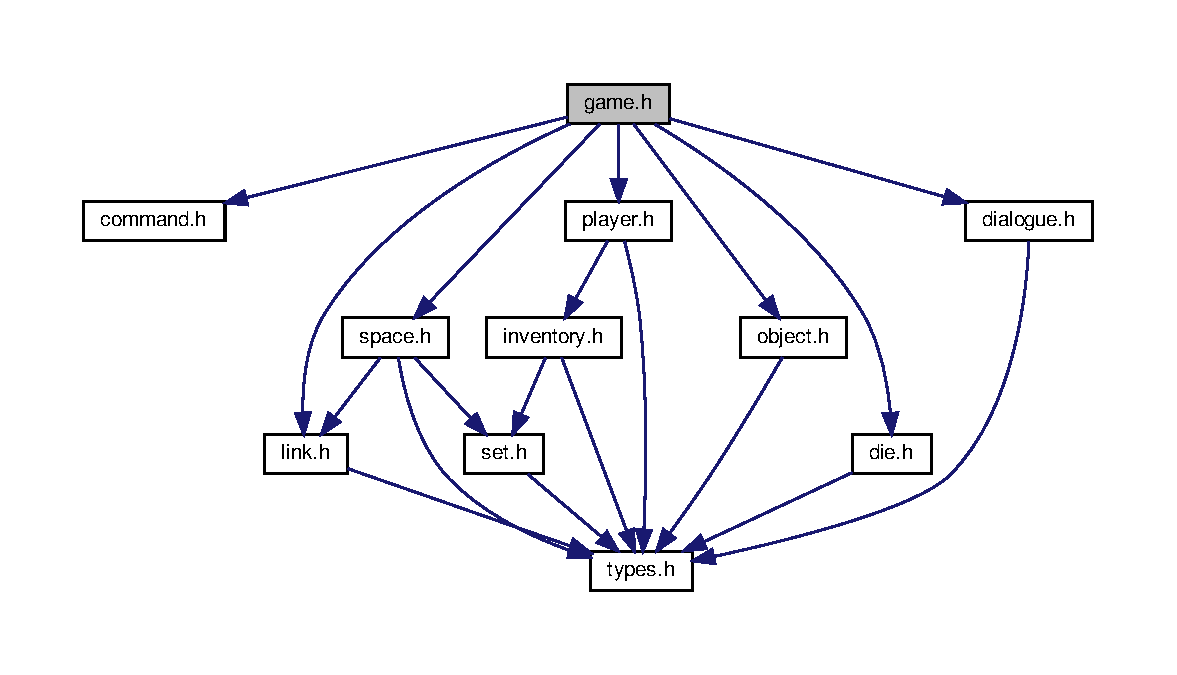
\includegraphics[width=350pt]{game_8h__incl}
\end{center}
\end{figure}
This graph shows which files directly or indirectly include this file\+:
\nopagebreak
\begin{figure}[H]
\begin{center}
\leavevmode
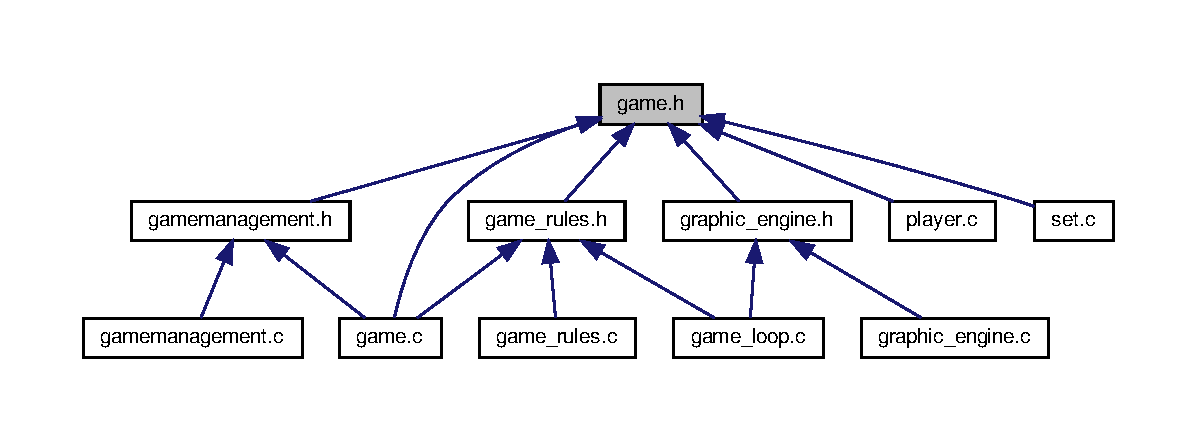
\includegraphics[width=350pt]{game_8h__dep__incl}
\end{center}
\end{figure}
\subsection*{Typedefs}
\begin{DoxyCompactItemize}
\item 
\mbox{\Hypertarget{game_8h_a57156d39c530aec3fba3a9dad8c2dc6a}\label{game_8h_a57156d39c530aec3fba3a9dad8c2dc6a}} 
typedef struct \hyperlink{struct__Game}{\+\_\+\+Game} \hyperlink{game_8h_a57156d39c530aec3fba3a9dad8c2dc6a}{Game}
\begin{DoxyCompactList}\small\item\em defines the game structure \end{DoxyCompactList}\end{DoxyCompactItemize}
\subsection*{Functions}
\begin{DoxyCompactItemize}
\item 
\hyperlink{game_8h_a57156d39c530aec3fba3a9dad8c2dc6a}{Game} $\ast$ \hyperlink{game_8h_a1cdbe3f06b9bf49eb5e334a22ad3b2b9}{game\+\_\+create} ()
\begin{DoxyCompactList}\small\item\em create a game \end{DoxyCompactList}\item 
\hyperlink{types_8h_a32c27cc471df37f4fc818d65de0a56c4}{S\+T\+A\+T\+US} \hyperlink{game_8h_afc77f90739be0fd45b7f5616e543bfae}{game\+\_\+create\+\_\+from\+\_\+file} (\hyperlink{game_8h_a57156d39c530aec3fba3a9dad8c2dc6a}{Game} $\ast$game, char $\ast$filename)
\begin{DoxyCompactList}\small\item\em create file in game \end{DoxyCompactList}\item 
\hyperlink{types_8h_a32c27cc471df37f4fc818d65de0a56c4}{S\+T\+A\+T\+US} \hyperlink{game_8h_a005b4f436300333e7fff8fba2027337e}{game\+\_\+update} (\hyperlink{game_8h_a57156d39c530aec3fba3a9dad8c2dc6a}{Game} $\ast$game, \hyperlink{command_8h_a0473597db8c45c0289b6b8e2f8abbe32}{T\+\_\+\+Command} cmd)
\begin{DoxyCompactList}\small\item\em update the game with a comand \end{DoxyCompactList}\item 
\hyperlink{types_8h_a32c27cc471df37f4fc818d65de0a56c4}{S\+T\+A\+T\+US} \hyperlink{game_8h_a0736924a1235c0e6fe9b6d91c2a12af8}{game\+\_\+destroy} (\hyperlink{game_8h_a57156d39c530aec3fba3a9dad8c2dc6a}{Game} $\ast$game)
\begin{DoxyCompactList}\small\item\em destroy game \end{DoxyCompactList}\item 
\hyperlink{types_8h_a3e5b8192e7d9ffaf3542f1210aec18dd}{B\+O\+OL} \hyperlink{game_8h_aa6efe0650af110bbd84e742cc8046d93}{game\+\_\+is\+\_\+over} (\hyperlink{game_8h_a57156d39c530aec3fba3a9dad8c2dc6a}{Game} $\ast$game)
\begin{DoxyCompactList}\small\item\em Tells if game is over. \end{DoxyCompactList}\item 
void \hyperlink{game_8h_a108f413649a6dc99d3ffeed092dc15f5}{game\+\_\+print\+\_\+screen} (\hyperlink{game_8h_a57156d39c530aec3fba3a9dad8c2dc6a}{Game} $\ast$game)
\begin{DoxyCompactList}\small\item\em prints game in screen \end{DoxyCompactList}\item 
void \hyperlink{game_8h_a33a5ed8937423f8c012df3cedad4fa4c}{game\+\_\+print\+\_\+data} (\hyperlink{game_8h_a57156d39c530aec3fba3a9dad8c2dc6a}{Game} $\ast$game)
\begin{DoxyCompactList}\small\item\em prints data in screen \end{DoxyCompactList}\item 
\hyperlink{space_8h_a67533ffc2b70463baecc38fb0629bbfc}{Space} $\ast$ \hyperlink{game_8h_a69d94da9d27b542d3ebdeb8b60f1f2dc}{game\+\_\+get\+\_\+space} (\hyperlink{game_8h_a57156d39c530aec3fba3a9dad8c2dc6a}{Game} $\ast$game, \hyperlink{types_8h_a845e604fb28f7e3d97549da3448149d3}{Id} id)
\begin{DoxyCompactList}\small\item\em get space in game \end{DoxyCompactList}\item 
\hyperlink{types_8h_a845e604fb28f7e3d97549da3448149d3}{Id} \hyperlink{game_8h_ac6a628f2106f81c37d0e83c67920615f}{game\+\_\+get\+\_\+player\+\_\+location} (\hyperlink{game_8h_a57156d39c530aec3fba3a9dad8c2dc6a}{Game} $\ast$game)
\begin{DoxyCompactList}\small\item\em get player location in game \end{DoxyCompactList}\item 
\hyperlink{types_8h_a845e604fb28f7e3d97549da3448149d3}{Id} \hyperlink{game_8h_a125e39363568d37bdb1c404766ad1c0e}{game\+\_\+get\+\_\+player\+\_\+object} (\hyperlink{game_8h_a57156d39c530aec3fba3a9dad8c2dc6a}{Game} $\ast$game)
\begin{DoxyCompactList}\small\item\em get player object in game \end{DoxyCompactList}\item 
\hyperlink{types_8h_a845e604fb28f7e3d97549da3448149d3}{Id} \hyperlink{game_8h_aa84eca5a1131daafd7acbf74263b6f82}{game\+\_\+get\+\_\+object\+\_\+location} (\hyperlink{game_8h_a57156d39c530aec3fba3a9dad8c2dc6a}{Game} $\ast$game, \hyperlink{types_8h_a845e604fb28f7e3d97549da3448149d3}{Id} id)
\begin{DoxyCompactList}\small\item\em get objcet location in game \end{DoxyCompactList}\item 
\hyperlink{command_8h_a0473597db8c45c0289b6b8e2f8abbe32}{T\+\_\+\+Command} \hyperlink{game_8h_ac35df1afdade2b7659ebbcfeca1f0c35}{game\+\_\+get\+\_\+last\+\_\+command} (\hyperlink{game_8h_a57156d39c530aec3fba3a9dad8c2dc6a}{Game} $\ast$game)
\begin{DoxyCompactList}\small\item\em get last command in the game \end{DoxyCompactList}\item 
int \hyperlink{game_8h_a8a4f34821dc1203eabc71e89cb9d6506}{game\+\_\+get\+\_\+die\+\_\+value} (\hyperlink{game_8h_a57156d39c530aec3fba3a9dad8c2dc6a}{Game} $\ast$game)
\begin{DoxyCompactList}\small\item\em get die value \end{DoxyCompactList}\item 
\hyperlink{types_8h_a32c27cc471df37f4fc818d65de0a56c4}{S\+T\+A\+T\+US} \hyperlink{game_8h_a15cf6b8e605b1605cebaf83e686c60a2}{game\+\_\+get\+\_\+callback\+\_\+status} (\hyperlink{game_8h_a57156d39c530aec3fba3a9dad8c2dc6a}{Game} $\ast$game)
\begin{DoxyCompactList}\small\item\em get callback \end{DoxyCompactList}\item 
\hyperlink{types_8h_a32c27cc471df37f4fc818d65de0a56c4}{S\+T\+A\+T\+US} \hyperlink{game_8h_a9597a8e456aa74db536e87d56f56c3b4}{game\+\_\+add\+\_\+object} (\hyperlink{game_8h_a57156d39c530aec3fba3a9dad8c2dc6a}{Game} $\ast$game, \hyperlink{object_8h_a7f8bbcda919b65ce67f92fba08e0212f}{Object} $\ast$object)
\begin{DoxyCompactList}\small\item\em add an object to the game \end{DoxyCompactList}\item 
\hyperlink{types_8h_a845e604fb28f7e3d97549da3448149d3}{Id} \hyperlink{game_8h_a108b794acf67ee339d4e9a836eaa5e6b}{game\+\_\+get\+\_\+object\+Id} (\hyperlink{game_8h_a57156d39c530aec3fba3a9dad8c2dc6a}{Game} $\ast$game, int i)
\begin{DoxyCompactList}\small\item\em get the id of object in the game \end{DoxyCompactList}\item 
\hyperlink{object_8h_a7f8bbcda919b65ce67f92fba08e0212f}{Object} $\ast$ \hyperlink{game_8h_a5c49f8a836a21a488e7a693f6b427eab}{game\+\_\+get\+\_\+object} (\hyperlink{game_8h_a57156d39c530aec3fba3a9dad8c2dc6a}{Game} $\ast$g, \hyperlink{types_8h_a845e604fb28f7e3d97549da3448149d3}{Id} id)
\begin{DoxyCompactList}\small\item\em get the object in the game \end{DoxyCompactList}\item 
\hyperlink{link_8h_ae3b299941e67be6971bfd64a25505eff}{Link} $\ast$ \hyperlink{game_8h_a1064ec927b8c33cf55982b73845db7d3}{game\+\_\+get\+\_\+link} (\hyperlink{game_8h_a57156d39c530aec3fba3a9dad8c2dc6a}{Game} $\ast$game, \hyperlink{types_8h_a845e604fb28f7e3d97549da3448149d3}{Id} id)
\begin{DoxyCompactList}\small\item\em get the link in the game to be able to go to another space \end{DoxyCompactList}\item 
\hyperlink{object_8h_a7f8bbcda919b65ce67f92fba08e0212f}{Object} $\ast$ \hyperlink{game_8h_a4be371129095096aae4b0d9006ecf2b2}{game\+\_\+get\+\_\+objectbypos} (\hyperlink{game_8h_a57156d39c530aec3fba3a9dad8c2dc6a}{Game} $\ast$game, \hyperlink{types_8h_a845e604fb28f7e3d97549da3448149d3}{Id} i)
\begin{DoxyCompactList}\small\item\em get the object of id i \end{DoxyCompactList}\item 
\hyperlink{types_8h_a32c27cc471df37f4fc818d65de0a56c4}{S\+T\+A\+T\+US} \hyperlink{game_8h_a9a35b366559b5255c27f01db2da752b2}{game\+\_\+set\+\_\+objectbypos} (\hyperlink{game_8h_a57156d39c530aec3fba3a9dad8c2dc6a}{Game} $\ast$game, \hyperlink{types_8h_a845e604fb28f7e3d97549da3448149d3}{Id} i, \hyperlink{object_8h_a7f8bbcda919b65ce67f92fba08e0212f}{Object} $\ast$object)
\begin{DoxyCompactList}\small\item\em set the object of id i in the game \end{DoxyCompactList}\item 
\hyperlink{player_8h_af30e2030635a69690f85e48bc6ef202f}{Player} $\ast$ \hyperlink{game_8h_af46efd507d797aec6da90d08aa592e32}{game\+\_\+get\+\_\+player} (\hyperlink{game_8h_a57156d39c530aec3fba3a9dad8c2dc6a}{Game} $\ast$game)
\begin{DoxyCompactList}\small\item\em get player \end{DoxyCompactList}\item 
\hyperlink{space_8h_a67533ffc2b70463baecc38fb0629bbfc}{Space} $\ast$ \hyperlink{game_8h_a27d440d8ef093faae7e78f0f2a35bf7f}{game\+\_\+get\+\_\+spacebypos} (\hyperlink{game_8h_a57156d39c530aec3fba3a9dad8c2dc6a}{Game} $\ast$game, \hyperlink{types_8h_a845e604fb28f7e3d97549da3448149d3}{Id} i)
\begin{DoxyCompactList}\small\item\em get spaces of id i \end{DoxyCompactList}\item 
\hyperlink{types_8h_a32c27cc471df37f4fc818d65de0a56c4}{S\+T\+A\+T\+US} \hyperlink{game_8h_a3815eedebbe3d5f514152f8e28b4432e}{game\+\_\+set\+\_\+spacebypos} (\hyperlink{game_8h_a57156d39c530aec3fba3a9dad8c2dc6a}{Game} $\ast$game, \hyperlink{types_8h_a845e604fb28f7e3d97549da3448149d3}{Id} i, \hyperlink{space_8h_a67533ffc2b70463baecc38fb0629bbfc}{Space} $\ast$space)
\begin{DoxyCompactList}\small\item\em set spaces of id i in the game \end{DoxyCompactList}\item 
\hyperlink{link_8h_ae3b299941e67be6971bfd64a25505eff}{Link} $\ast$ \hyperlink{game_8h_a0ae52e043aae52a695ce7ef58a2d6b2a}{game\+\_\+get\+\_\+linkbypos} (\hyperlink{game_8h_a57156d39c530aec3fba3a9dad8c2dc6a}{Game} $\ast$game, \hyperlink{types_8h_a845e604fb28f7e3d97549da3448149d3}{Id} i)
\begin{DoxyCompactList}\small\item\em set links of id i in the game \end{DoxyCompactList}\item 
\hyperlink{types_8h_a32c27cc471df37f4fc818d65de0a56c4}{S\+T\+A\+T\+US} \hyperlink{game_8h_ac250ef059d55d7e51669ba832f02b544}{game\+\_\+set\+\_\+linkbypos} (\hyperlink{game_8h_a57156d39c530aec3fba3a9dad8c2dc6a}{Game} $\ast$game, \hyperlink{types_8h_a845e604fb28f7e3d97549da3448149d3}{Id} i, \hyperlink{link_8h_ae3b299941e67be6971bfd64a25505eff}{Link} $\ast$link)
\begin{DoxyCompactList}\small\item\em get links of id i in the game \end{DoxyCompactList}\item 
\hyperlink{types_8h_a32c27cc471df37f4fc818d65de0a56c4}{S\+T\+A\+T\+US} \hyperlink{game_8h_a48ef5745474ef224f39ed913c3a176e4}{game\+\_\+set\+\_\+objdsc} (\hyperlink{game_8h_a57156d39c530aec3fba3a9dad8c2dc6a}{Game} $\ast$game, char $\ast$objdsc)
\begin{DoxyCompactList}\small\item\em set objects of id i in the game \end{DoxyCompactList}\item 
char $\ast$ \hyperlink{game_8h_a83d23be85660b3a92d73268ba07638ea}{game\+\_\+get\+\_\+objdsc} (\hyperlink{game_8h_a57156d39c530aec3fba3a9dad8c2dc6a}{Game} $\ast$game)
\begin{DoxyCompactList}\small\item\em get the name of objects \end{DoxyCompactList}\end{DoxyCompactItemize}


\subsection{Detailed Description}
It defines the game interface for each command. 

\begin{DoxyAuthor}{Author}
\end{DoxyAuthor}
\begin{DoxyVersion}{Version}
1.\+0 
\end{DoxyVersion}
\begin{DoxyDate}{Date}
04-\/02-\/2019 
\end{DoxyDate}
\begin{DoxyCopyright}{Copyright}
G\+NU Public License 
\end{DoxyCopyright}


\subsection{Function Documentation}
\mbox{\Hypertarget{game_8h_a9597a8e456aa74db536e87d56f56c3b4}\label{game_8h_a9597a8e456aa74db536e87d56f56c3b4}} 
\index{game.\+h@{game.\+h}!game\+\_\+add\+\_\+object@{game\+\_\+add\+\_\+object}}
\index{game\+\_\+add\+\_\+object@{game\+\_\+add\+\_\+object}!game.\+h@{game.\+h}}
\subsubsection{\texorpdfstring{game\+\_\+add\+\_\+object()}{game\_add\_object()}}
{\footnotesize\ttfamily \hyperlink{types_8h_a32c27cc471df37f4fc818d65de0a56c4}{S\+T\+A\+T\+US} game\+\_\+add\+\_\+object (\begin{DoxyParamCaption}\item[{\hyperlink{game_8h_a57156d39c530aec3fba3a9dad8c2dc6a}{Game} $\ast$}]{game,  }\item[{\hyperlink{object_8h_a7f8bbcda919b65ce67f92fba08e0212f}{Object} $\ast$}]{object }\end{DoxyParamCaption})}



add an object to the game 


\begin{DoxyParams}{Parameters}
{\em game} & \\
\hline
{\em object} & \\
\hline
\end{DoxyParams}
\begin{DoxyReturn}{Returns}
OK, or E\+R\+R\+OR 
\end{DoxyReturn}
\mbox{\Hypertarget{game_8h_a1cdbe3f06b9bf49eb5e334a22ad3b2b9}\label{game_8h_a1cdbe3f06b9bf49eb5e334a22ad3b2b9}} 
\index{game.\+h@{game.\+h}!game\+\_\+create@{game\+\_\+create}}
\index{game\+\_\+create@{game\+\_\+create}!game.\+h@{game.\+h}}
\subsubsection{\texorpdfstring{game\+\_\+create()}{game\_create()}}
{\footnotesize\ttfamily \hyperlink{game_8h_a57156d39c530aec3fba3a9dad8c2dc6a}{Game}$\ast$ game\+\_\+create (\begin{DoxyParamCaption}{ }\end{DoxyParamCaption})}



create a game 

\begin{DoxyReturn}{Returns}
OK, or E\+R\+R\+OR 
\end{DoxyReturn}
\mbox{\Hypertarget{game_8h_afc77f90739be0fd45b7f5616e543bfae}\label{game_8h_afc77f90739be0fd45b7f5616e543bfae}} 
\index{game.\+h@{game.\+h}!game\+\_\+create\+\_\+from\+\_\+file@{game\+\_\+create\+\_\+from\+\_\+file}}
\index{game\+\_\+create\+\_\+from\+\_\+file@{game\+\_\+create\+\_\+from\+\_\+file}!game.\+h@{game.\+h}}
\subsubsection{\texorpdfstring{game\+\_\+create\+\_\+from\+\_\+file()}{game\_create\_from\_file()}}
{\footnotesize\ttfamily \hyperlink{types_8h_a32c27cc471df37f4fc818d65de0a56c4}{S\+T\+A\+T\+US} game\+\_\+create\+\_\+from\+\_\+file (\begin{DoxyParamCaption}\item[{\hyperlink{game_8h_a57156d39c530aec3fba3a9dad8c2dc6a}{Game} $\ast$}]{game,  }\item[{char $\ast$}]{filename }\end{DoxyParamCaption})}



create file in game 


\begin{DoxyParams}{Parameters}
{\em game} & \\
\hline
{\em filename} & \\
\hline
\end{DoxyParams}
\begin{DoxyReturn}{Returns}
OK, or E\+R\+R\+OR 
\end{DoxyReturn}
\mbox{\Hypertarget{game_8h_a0736924a1235c0e6fe9b6d91c2a12af8}\label{game_8h_a0736924a1235c0e6fe9b6d91c2a12af8}} 
\index{game.\+h@{game.\+h}!game\+\_\+destroy@{game\+\_\+destroy}}
\index{game\+\_\+destroy@{game\+\_\+destroy}!game.\+h@{game.\+h}}
\subsubsection{\texorpdfstring{game\+\_\+destroy()}{game\_destroy()}}
{\footnotesize\ttfamily \hyperlink{types_8h_a32c27cc471df37f4fc818d65de0a56c4}{S\+T\+A\+T\+US} game\+\_\+destroy (\begin{DoxyParamCaption}\item[{\hyperlink{game_8h_a57156d39c530aec3fba3a9dad8c2dc6a}{Game} $\ast$}]{game }\end{DoxyParamCaption})}



destroy game 


\begin{DoxyParams}{Parameters}
{\em game} & \\
\hline
\end{DoxyParams}
\begin{DoxyReturn}{Returns}
OK, or E\+R\+R\+OR 
\end{DoxyReturn}
\mbox{\Hypertarget{game_8h_a15cf6b8e605b1605cebaf83e686c60a2}\label{game_8h_a15cf6b8e605b1605cebaf83e686c60a2}} 
\index{game.\+h@{game.\+h}!game\+\_\+get\+\_\+callback\+\_\+status@{game\+\_\+get\+\_\+callback\+\_\+status}}
\index{game\+\_\+get\+\_\+callback\+\_\+status@{game\+\_\+get\+\_\+callback\+\_\+status}!game.\+h@{game.\+h}}
\subsubsection{\texorpdfstring{game\+\_\+get\+\_\+callback\+\_\+status()}{game\_get\_callback\_status()}}
{\footnotesize\ttfamily \hyperlink{types_8h_a32c27cc471df37f4fc818d65de0a56c4}{S\+T\+A\+T\+US} game\+\_\+get\+\_\+callback\+\_\+status (\begin{DoxyParamCaption}\item[{\hyperlink{game_8h_a57156d39c530aec3fba3a9dad8c2dc6a}{Game} $\ast$}]{game }\end{DoxyParamCaption})}



get callback 


\begin{DoxyParams}{Parameters}
{\em game} & \\
\hline
\end{DoxyParams}
\begin{DoxyReturn}{Returns}
OK, or E\+R\+R\+OR
\end{DoxyReturn}

\begin{DoxyParams}{Parameters}
{\em game} & \\
\hline
\end{DoxyParams}
\begin{DoxyReturn}{Returns}
OK or E\+R\+R\+OR 
\end{DoxyReturn}
\mbox{\Hypertarget{game_8h_a8a4f34821dc1203eabc71e89cb9d6506}\label{game_8h_a8a4f34821dc1203eabc71e89cb9d6506}} 
\index{game.\+h@{game.\+h}!game\+\_\+get\+\_\+die\+\_\+value@{game\+\_\+get\+\_\+die\+\_\+value}}
\index{game\+\_\+get\+\_\+die\+\_\+value@{game\+\_\+get\+\_\+die\+\_\+value}!game.\+h@{game.\+h}}
\subsubsection{\texorpdfstring{game\+\_\+get\+\_\+die\+\_\+value()}{game\_get\_die\_value()}}
{\footnotesize\ttfamily int game\+\_\+get\+\_\+die\+\_\+value (\begin{DoxyParamCaption}\item[{\hyperlink{game_8h_a57156d39c530aec3fba3a9dad8c2dc6a}{Game} $\ast$}]{game }\end{DoxyParamCaption})}



get die value 


\begin{DoxyParams}{Parameters}
{\em game} & \\
\hline
\end{DoxyParams}
\begin{DoxyReturn}{Returns}
the die valuie(int) or -\/1 in case of error 
\end{DoxyReturn}
\mbox{\Hypertarget{game_8h_ac35df1afdade2b7659ebbcfeca1f0c35}\label{game_8h_ac35df1afdade2b7659ebbcfeca1f0c35}} 
\index{game.\+h@{game.\+h}!game\+\_\+get\+\_\+last\+\_\+command@{game\+\_\+get\+\_\+last\+\_\+command}}
\index{game\+\_\+get\+\_\+last\+\_\+command@{game\+\_\+get\+\_\+last\+\_\+command}!game.\+h@{game.\+h}}
\subsubsection{\texorpdfstring{game\+\_\+get\+\_\+last\+\_\+command()}{game\_get\_last\_command()}}
{\footnotesize\ttfamily \hyperlink{command_8h_a0473597db8c45c0289b6b8e2f8abbe32}{T\+\_\+\+Command} game\+\_\+get\+\_\+last\+\_\+command (\begin{DoxyParamCaption}\item[{\hyperlink{game_8h_a57156d39c530aec3fba3a9dad8c2dc6a}{Game} $\ast$}]{game }\end{DoxyParamCaption})}



get last command in the game 


\begin{DoxyParams}{Parameters}
{\em game} & \\
\hline
\end{DoxyParams}
\begin{DoxyReturn}{Returns}
id or in case of error N\+U\+LL 
\end{DoxyReturn}
\mbox{\Hypertarget{game_8h_a1064ec927b8c33cf55982b73845db7d3}\label{game_8h_a1064ec927b8c33cf55982b73845db7d3}} 
\index{game.\+h@{game.\+h}!game\+\_\+get\+\_\+link@{game\+\_\+get\+\_\+link}}
\index{game\+\_\+get\+\_\+link@{game\+\_\+get\+\_\+link}!game.\+h@{game.\+h}}
\subsubsection{\texorpdfstring{game\+\_\+get\+\_\+link()}{game\_get\_link()}}
{\footnotesize\ttfamily \hyperlink{link_8h_ae3b299941e67be6971bfd64a25505eff}{Link}$\ast$ game\+\_\+get\+\_\+link (\begin{DoxyParamCaption}\item[{\hyperlink{game_8h_a57156d39c530aec3fba3a9dad8c2dc6a}{Game} $\ast$}]{game,  }\item[{\hyperlink{types_8h_a845e604fb28f7e3d97549da3448149d3}{Id}}]{id }\end{DoxyParamCaption})}



get the link in the game to be able to go to another space 


\begin{DoxyParams}{Parameters}
{\em game} & \\
\hline
{\em id} & \\
\hline
\end{DoxyParams}
\begin{DoxyReturn}{Returns}
link or in case of error N\+U\+LL 
\end{DoxyReturn}
\mbox{\Hypertarget{game_8h_a0ae52e043aae52a695ce7ef58a2d6b2a}\label{game_8h_a0ae52e043aae52a695ce7ef58a2d6b2a}} 
\index{game.\+h@{game.\+h}!game\+\_\+get\+\_\+linkbypos@{game\+\_\+get\+\_\+linkbypos}}
\index{game\+\_\+get\+\_\+linkbypos@{game\+\_\+get\+\_\+linkbypos}!game.\+h@{game.\+h}}
\subsubsection{\texorpdfstring{game\+\_\+get\+\_\+linkbypos()}{game\_get\_linkbypos()}}
{\footnotesize\ttfamily \hyperlink{link_8h_ae3b299941e67be6971bfd64a25505eff}{Link}$\ast$ game\+\_\+get\+\_\+linkbypos (\begin{DoxyParamCaption}\item[{\hyperlink{game_8h_a57156d39c530aec3fba3a9dad8c2dc6a}{Game} $\ast$}]{game,  }\item[{\hyperlink{types_8h_a845e604fb28f7e3d97549da3448149d3}{Id}}]{i }\end{DoxyParamCaption})}



set links of id i in the game 


\begin{DoxyParams}{Parameters}
{\em game} & \\
\hline
{\em i} & \\
\hline
\end{DoxyParams}
\begin{DoxyReturn}{Returns}
link or in case of error N\+U\+LL 
\end{DoxyReturn}
\mbox{\Hypertarget{game_8h_a83d23be85660b3a92d73268ba07638ea}\label{game_8h_a83d23be85660b3a92d73268ba07638ea}} 
\index{game.\+h@{game.\+h}!game\+\_\+get\+\_\+objdsc@{game\+\_\+get\+\_\+objdsc}}
\index{game\+\_\+get\+\_\+objdsc@{game\+\_\+get\+\_\+objdsc}!game.\+h@{game.\+h}}
\subsubsection{\texorpdfstring{game\+\_\+get\+\_\+objdsc()}{game\_get\_objdsc()}}
{\footnotesize\ttfamily char$\ast$ game\+\_\+get\+\_\+objdsc (\begin{DoxyParamCaption}\item[{\hyperlink{game_8h_a57156d39c530aec3fba3a9dad8c2dc6a}{Game} $\ast$}]{game }\end{DoxyParamCaption})}



get the name of objects 


\begin{DoxyParams}{Parameters}
{\em game} & \\
\hline
\end{DoxyParams}
\begin{DoxyReturn}{Returns}
object or in case of error N\+U\+LL 
\end{DoxyReturn}
\mbox{\Hypertarget{game_8h_a5c49f8a836a21a488e7a693f6b427eab}\label{game_8h_a5c49f8a836a21a488e7a693f6b427eab}} 
\index{game.\+h@{game.\+h}!game\+\_\+get\+\_\+object@{game\+\_\+get\+\_\+object}}
\index{game\+\_\+get\+\_\+object@{game\+\_\+get\+\_\+object}!game.\+h@{game.\+h}}
\subsubsection{\texorpdfstring{game\+\_\+get\+\_\+object()}{game\_get\_object()}}
{\footnotesize\ttfamily \hyperlink{object_8h_a7f8bbcda919b65ce67f92fba08e0212f}{Object}$\ast$ game\+\_\+get\+\_\+object (\begin{DoxyParamCaption}\item[{\hyperlink{game_8h_a57156d39c530aec3fba3a9dad8c2dc6a}{Game} $\ast$}]{g,  }\item[{\hyperlink{types_8h_a845e604fb28f7e3d97549da3448149d3}{Id}}]{id }\end{DoxyParamCaption})}



get the object in the game 


\begin{DoxyParams}{Parameters}
{\em g} & \\
\hline
{\em id} & \\
\hline
\end{DoxyParams}
\begin{DoxyReturn}{Returns}
object or in case of error N\+U\+LL
\end{DoxyReturn}

\begin{DoxyParams}{Parameters}
{\em g} & \\
\hline
{\em id} & \\
\hline
\end{DoxyParams}
\begin{DoxyReturn}{Returns}
id or in case of error N\+U\+LL 
\end{DoxyReturn}
\mbox{\Hypertarget{game_8h_aa84eca5a1131daafd7acbf74263b6f82}\label{game_8h_aa84eca5a1131daafd7acbf74263b6f82}} 
\index{game.\+h@{game.\+h}!game\+\_\+get\+\_\+object\+\_\+location@{game\+\_\+get\+\_\+object\+\_\+location}}
\index{game\+\_\+get\+\_\+object\+\_\+location@{game\+\_\+get\+\_\+object\+\_\+location}!game.\+h@{game.\+h}}
\subsubsection{\texorpdfstring{game\+\_\+get\+\_\+object\+\_\+location()}{game\_get\_object\_location()}}
{\footnotesize\ttfamily \hyperlink{types_8h_a845e604fb28f7e3d97549da3448149d3}{Id} game\+\_\+get\+\_\+object\+\_\+location (\begin{DoxyParamCaption}\item[{\hyperlink{game_8h_a57156d39c530aec3fba3a9dad8c2dc6a}{Game} $\ast$}]{game,  }\item[{\hyperlink{types_8h_a845e604fb28f7e3d97549da3448149d3}{Id}}]{id }\end{DoxyParamCaption})}



get objcet location in game 


\begin{DoxyParams}{Parameters}
{\em game} & \\
\hline
{\em id} & \\
\hline
\end{DoxyParams}
\begin{DoxyReturn}{Returns}
id or in case of error N\+U\+LL 
\end{DoxyReturn}
\mbox{\Hypertarget{game_8h_a4be371129095096aae4b0d9006ecf2b2}\label{game_8h_a4be371129095096aae4b0d9006ecf2b2}} 
\index{game.\+h@{game.\+h}!game\+\_\+get\+\_\+objectbypos@{game\+\_\+get\+\_\+objectbypos}}
\index{game\+\_\+get\+\_\+objectbypos@{game\+\_\+get\+\_\+objectbypos}!game.\+h@{game.\+h}}
\subsubsection{\texorpdfstring{game\+\_\+get\+\_\+objectbypos()}{game\_get\_objectbypos()}}
{\footnotesize\ttfamily \hyperlink{object_8h_a7f8bbcda919b65ce67f92fba08e0212f}{Object}$\ast$ game\+\_\+get\+\_\+objectbypos (\begin{DoxyParamCaption}\item[{\hyperlink{game_8h_a57156d39c530aec3fba3a9dad8c2dc6a}{Game} $\ast$}]{game,  }\item[{\hyperlink{types_8h_a845e604fb28f7e3d97549da3448149d3}{Id}}]{i }\end{DoxyParamCaption})}



get the object of id i 


\begin{DoxyParams}{Parameters}
{\em game} & \\
\hline
{\em i} & \\
\hline
\end{DoxyParams}
\begin{DoxyReturn}{Returns}
object or in case of error N\+U\+LL 
\end{DoxyReturn}
\mbox{\Hypertarget{game_8h_a108b794acf67ee339d4e9a836eaa5e6b}\label{game_8h_a108b794acf67ee339d4e9a836eaa5e6b}} 
\index{game.\+h@{game.\+h}!game\+\_\+get\+\_\+object\+Id@{game\+\_\+get\+\_\+object\+Id}}
\index{game\+\_\+get\+\_\+object\+Id@{game\+\_\+get\+\_\+object\+Id}!game.\+h@{game.\+h}}
\subsubsection{\texorpdfstring{game\+\_\+get\+\_\+object\+Id()}{game\_get\_objectId()}}
{\footnotesize\ttfamily \hyperlink{types_8h_a845e604fb28f7e3d97549da3448149d3}{Id} game\+\_\+get\+\_\+object\+Id (\begin{DoxyParamCaption}\item[{\hyperlink{game_8h_a57156d39c530aec3fba3a9dad8c2dc6a}{Game} $\ast$}]{game,  }\item[{int}]{i }\end{DoxyParamCaption})}



get the id of object in the game 


\begin{DoxyParams}{Parameters}
{\em game} & \\
\hline
{\em i} & \\
\hline
\end{DoxyParams}
\begin{DoxyReturn}{Returns}
id or in case of error N\+U\+LL 
\end{DoxyReturn}
\mbox{\Hypertarget{game_8h_af46efd507d797aec6da90d08aa592e32}\label{game_8h_af46efd507d797aec6da90d08aa592e32}} 
\index{game.\+h@{game.\+h}!game\+\_\+get\+\_\+player@{game\+\_\+get\+\_\+player}}
\index{game\+\_\+get\+\_\+player@{game\+\_\+get\+\_\+player}!game.\+h@{game.\+h}}
\subsubsection{\texorpdfstring{game\+\_\+get\+\_\+player()}{game\_get\_player()}}
{\footnotesize\ttfamily \hyperlink{player_8h_af30e2030635a69690f85e48bc6ef202f}{Player}$\ast$ game\+\_\+get\+\_\+player (\begin{DoxyParamCaption}\item[{\hyperlink{game_8h_a57156d39c530aec3fba3a9dad8c2dc6a}{Game} $\ast$}]{game }\end{DoxyParamCaption})}



get player 


\begin{DoxyParams}{Parameters}
{\em game} & \\
\hline
\end{DoxyParams}
\begin{DoxyReturn}{Returns}
player or in case of error N\+U\+LL 
\end{DoxyReturn}
\mbox{\Hypertarget{game_8h_ac6a628f2106f81c37d0e83c67920615f}\label{game_8h_ac6a628f2106f81c37d0e83c67920615f}} 
\index{game.\+h@{game.\+h}!game\+\_\+get\+\_\+player\+\_\+location@{game\+\_\+get\+\_\+player\+\_\+location}}
\index{game\+\_\+get\+\_\+player\+\_\+location@{game\+\_\+get\+\_\+player\+\_\+location}!game.\+h@{game.\+h}}
\subsubsection{\texorpdfstring{game\+\_\+get\+\_\+player\+\_\+location()}{game\_get\_player\_location()}}
{\footnotesize\ttfamily \hyperlink{types_8h_a845e604fb28f7e3d97549da3448149d3}{Id} game\+\_\+get\+\_\+player\+\_\+location (\begin{DoxyParamCaption}\item[{\hyperlink{game_8h_a57156d39c530aec3fba3a9dad8c2dc6a}{Game} $\ast$}]{game }\end{DoxyParamCaption})}



get player location in game 


\begin{DoxyParams}{Parameters}
{\em game} & \\
\hline
\end{DoxyParams}
\begin{DoxyReturn}{Returns}
id or in case of error N\+U\+LL 
\end{DoxyReturn}
\mbox{\Hypertarget{game_8h_a125e39363568d37bdb1c404766ad1c0e}\label{game_8h_a125e39363568d37bdb1c404766ad1c0e}} 
\index{game.\+h@{game.\+h}!game\+\_\+get\+\_\+player\+\_\+object@{game\+\_\+get\+\_\+player\+\_\+object}}
\index{game\+\_\+get\+\_\+player\+\_\+object@{game\+\_\+get\+\_\+player\+\_\+object}!game.\+h@{game.\+h}}
\subsubsection{\texorpdfstring{game\+\_\+get\+\_\+player\+\_\+object()}{game\_get\_player\_object()}}
{\footnotesize\ttfamily \hyperlink{types_8h_a845e604fb28f7e3d97549da3448149d3}{Id} game\+\_\+get\+\_\+player\+\_\+object (\begin{DoxyParamCaption}\item[{\hyperlink{game_8h_a57156d39c530aec3fba3a9dad8c2dc6a}{Game} $\ast$}]{game }\end{DoxyParamCaption})}



get player object in game 


\begin{DoxyParams}{Parameters}
{\em game} & \\
\hline
\end{DoxyParams}
\begin{DoxyReturn}{Returns}
id or in case of error N\+U\+LL 
\end{DoxyReturn}
\mbox{\Hypertarget{game_8h_a69d94da9d27b542d3ebdeb8b60f1f2dc}\label{game_8h_a69d94da9d27b542d3ebdeb8b60f1f2dc}} 
\index{game.\+h@{game.\+h}!game\+\_\+get\+\_\+space@{game\+\_\+get\+\_\+space}}
\index{game\+\_\+get\+\_\+space@{game\+\_\+get\+\_\+space}!game.\+h@{game.\+h}}
\subsubsection{\texorpdfstring{game\+\_\+get\+\_\+space()}{game\_get\_space()}}
{\footnotesize\ttfamily \hyperlink{space_8h_a67533ffc2b70463baecc38fb0629bbfc}{Space}$\ast$ game\+\_\+get\+\_\+space (\begin{DoxyParamCaption}\item[{\hyperlink{game_8h_a57156d39c530aec3fba3a9dad8c2dc6a}{Game} $\ast$}]{game,  }\item[{\hyperlink{types_8h_a845e604fb28f7e3d97549da3448149d3}{Id}}]{id }\end{DoxyParamCaption})}



get space in game 


\begin{DoxyParams}{Parameters}
{\em game} & \\
\hline
{\em id} & \\
\hline
\end{DoxyParams}
\begin{DoxyReturn}{Returns}
space or in case of error N\+U\+LL 
\end{DoxyReturn}
\mbox{\Hypertarget{game_8h_a27d440d8ef093faae7e78f0f2a35bf7f}\label{game_8h_a27d440d8ef093faae7e78f0f2a35bf7f}} 
\index{game.\+h@{game.\+h}!game\+\_\+get\+\_\+spacebypos@{game\+\_\+get\+\_\+spacebypos}}
\index{game\+\_\+get\+\_\+spacebypos@{game\+\_\+get\+\_\+spacebypos}!game.\+h@{game.\+h}}
\subsubsection{\texorpdfstring{game\+\_\+get\+\_\+spacebypos()}{game\_get\_spacebypos()}}
{\footnotesize\ttfamily \hyperlink{space_8h_a67533ffc2b70463baecc38fb0629bbfc}{Space}$\ast$ game\+\_\+get\+\_\+spacebypos (\begin{DoxyParamCaption}\item[{\hyperlink{game_8h_a57156d39c530aec3fba3a9dad8c2dc6a}{Game} $\ast$}]{game,  }\item[{\hyperlink{types_8h_a845e604fb28f7e3d97549da3448149d3}{Id}}]{i }\end{DoxyParamCaption})}



get spaces of id i 


\begin{DoxyParams}{Parameters}
{\em game} & \\
\hline
{\em i} & \\
\hline
\end{DoxyParams}
\begin{DoxyReturn}{Returns}
player or in case of error N\+U\+LL 
\end{DoxyReturn}
\mbox{\Hypertarget{game_8h_aa6efe0650af110bbd84e742cc8046d93}\label{game_8h_aa6efe0650af110bbd84e742cc8046d93}} 
\index{game.\+h@{game.\+h}!game\+\_\+is\+\_\+over@{game\+\_\+is\+\_\+over}}
\index{game\+\_\+is\+\_\+over@{game\+\_\+is\+\_\+over}!game.\+h@{game.\+h}}
\subsubsection{\texorpdfstring{game\+\_\+is\+\_\+over()}{game\_is\_over()}}
{\footnotesize\ttfamily \hyperlink{types_8h_a3e5b8192e7d9ffaf3542f1210aec18dd}{B\+O\+OL} game\+\_\+is\+\_\+over (\begin{DoxyParamCaption}\item[{\hyperlink{game_8h_a57156d39c530aec3fba3a9dad8c2dc6a}{Game} $\ast$}]{game }\end{DoxyParamCaption})}



Tells if game is over. 


\begin{DoxyParams}{Parameters}
{\em game} & \\
\hline
\end{DoxyParams}
\begin{DoxyReturn}{Returns}
T\+R\+UE or F\+A\+L\+SE 
\end{DoxyReturn}
\mbox{\Hypertarget{game_8h_a33a5ed8937423f8c012df3cedad4fa4c}\label{game_8h_a33a5ed8937423f8c012df3cedad4fa4c}} 
\index{game.\+h@{game.\+h}!game\+\_\+print\+\_\+data@{game\+\_\+print\+\_\+data}}
\index{game\+\_\+print\+\_\+data@{game\+\_\+print\+\_\+data}!game.\+h@{game.\+h}}
\subsubsection{\texorpdfstring{game\+\_\+print\+\_\+data()}{game\_print\_data()}}
{\footnotesize\ttfamily void game\+\_\+print\+\_\+data (\begin{DoxyParamCaption}\item[{\hyperlink{game_8h_a57156d39c530aec3fba3a9dad8c2dc6a}{Game} $\ast$}]{game }\end{DoxyParamCaption})}



prints data in screen 


\begin{DoxyParams}{Parameters}
{\em game} & \\
\hline
\end{DoxyParams}
\begin{DoxyReturn}{Returns}
void 
\end{DoxyReturn}
\mbox{\Hypertarget{game_8h_a108f413649a6dc99d3ffeed092dc15f5}\label{game_8h_a108f413649a6dc99d3ffeed092dc15f5}} 
\index{game.\+h@{game.\+h}!game\+\_\+print\+\_\+screen@{game\+\_\+print\+\_\+screen}}
\index{game\+\_\+print\+\_\+screen@{game\+\_\+print\+\_\+screen}!game.\+h@{game.\+h}}
\subsubsection{\texorpdfstring{game\+\_\+print\+\_\+screen()}{game\_print\_screen()}}
{\footnotesize\ttfamily void game\+\_\+print\+\_\+screen (\begin{DoxyParamCaption}\item[{\hyperlink{game_8h_a57156d39c530aec3fba3a9dad8c2dc6a}{Game} $\ast$}]{game }\end{DoxyParamCaption})}



prints game in screen 


\begin{DoxyParams}{Parameters}
{\em game} & \\
\hline
\end{DoxyParams}
\begin{DoxyReturn}{Returns}
void 
\end{DoxyReturn}
\mbox{\Hypertarget{game_8h_ac250ef059d55d7e51669ba832f02b544}\label{game_8h_ac250ef059d55d7e51669ba832f02b544}} 
\index{game.\+h@{game.\+h}!game\+\_\+set\+\_\+linkbypos@{game\+\_\+set\+\_\+linkbypos}}
\index{game\+\_\+set\+\_\+linkbypos@{game\+\_\+set\+\_\+linkbypos}!game.\+h@{game.\+h}}
\subsubsection{\texorpdfstring{game\+\_\+set\+\_\+linkbypos()}{game\_set\_linkbypos()}}
{\footnotesize\ttfamily \hyperlink{types_8h_a32c27cc471df37f4fc818d65de0a56c4}{S\+T\+A\+T\+US} game\+\_\+set\+\_\+linkbypos (\begin{DoxyParamCaption}\item[{\hyperlink{game_8h_a57156d39c530aec3fba3a9dad8c2dc6a}{Game} $\ast$}]{game,  }\item[{\hyperlink{types_8h_a845e604fb28f7e3d97549da3448149d3}{Id}}]{i,  }\item[{\hyperlink{link_8h_ae3b299941e67be6971bfd64a25505eff}{Link} $\ast$}]{link }\end{DoxyParamCaption})}



get links of id i in the game 


\begin{DoxyParams}{Parameters}
{\em game} & \\
\hline
{\em i} & \\
\hline
{\em link} & \\
\hline
\end{DoxyParams}
\begin{DoxyReturn}{Returns}
OK or E\+R\+R\+OR 
\end{DoxyReturn}
\mbox{\Hypertarget{game_8h_a48ef5745474ef224f39ed913c3a176e4}\label{game_8h_a48ef5745474ef224f39ed913c3a176e4}} 
\index{game.\+h@{game.\+h}!game\+\_\+set\+\_\+objdsc@{game\+\_\+set\+\_\+objdsc}}
\index{game\+\_\+set\+\_\+objdsc@{game\+\_\+set\+\_\+objdsc}!game.\+h@{game.\+h}}
\subsubsection{\texorpdfstring{game\+\_\+set\+\_\+objdsc()}{game\_set\_objdsc()}}
{\footnotesize\ttfamily \hyperlink{types_8h_a32c27cc471df37f4fc818d65de0a56c4}{S\+T\+A\+T\+US} game\+\_\+set\+\_\+objdsc (\begin{DoxyParamCaption}\item[{\hyperlink{game_8h_a57156d39c530aec3fba3a9dad8c2dc6a}{Game} $\ast$}]{game,  }\item[{char $\ast$}]{objdsc }\end{DoxyParamCaption})}



set objects of id i in the game 


\begin{DoxyParams}{Parameters}
{\em game} & \\
\hline
{\em objdsc} & \\
\hline
\end{DoxyParams}
\begin{DoxyReturn}{Returns}
OK or E\+R\+R\+OR 
\end{DoxyReturn}
\mbox{\Hypertarget{game_8h_a9a35b366559b5255c27f01db2da752b2}\label{game_8h_a9a35b366559b5255c27f01db2da752b2}} 
\index{game.\+h@{game.\+h}!game\+\_\+set\+\_\+objectbypos@{game\+\_\+set\+\_\+objectbypos}}
\index{game\+\_\+set\+\_\+objectbypos@{game\+\_\+set\+\_\+objectbypos}!game.\+h@{game.\+h}}
\subsubsection{\texorpdfstring{game\+\_\+set\+\_\+objectbypos()}{game\_set\_objectbypos()}}
{\footnotesize\ttfamily \hyperlink{types_8h_a32c27cc471df37f4fc818d65de0a56c4}{S\+T\+A\+T\+US} game\+\_\+set\+\_\+objectbypos (\begin{DoxyParamCaption}\item[{\hyperlink{game_8h_a57156d39c530aec3fba3a9dad8c2dc6a}{Game} $\ast$}]{game,  }\item[{\hyperlink{types_8h_a845e604fb28f7e3d97549da3448149d3}{Id}}]{i,  }\item[{\hyperlink{object_8h_a7f8bbcda919b65ce67f92fba08e0212f}{Object} $\ast$}]{object }\end{DoxyParamCaption})}



set the object of id i in the game 


\begin{DoxyParams}{Parameters}
{\em game} & \\
\hline
{\em i} & \\
\hline
{\em object} & \\
\hline
\end{DoxyParams}
\begin{DoxyReturn}{Returns}
OK or E\+R\+R\+OR 
\end{DoxyReturn}
\mbox{\Hypertarget{game_8h_a3815eedebbe3d5f514152f8e28b4432e}\label{game_8h_a3815eedebbe3d5f514152f8e28b4432e}} 
\index{game.\+h@{game.\+h}!game\+\_\+set\+\_\+spacebypos@{game\+\_\+set\+\_\+spacebypos}}
\index{game\+\_\+set\+\_\+spacebypos@{game\+\_\+set\+\_\+spacebypos}!game.\+h@{game.\+h}}
\subsubsection{\texorpdfstring{game\+\_\+set\+\_\+spacebypos()}{game\_set\_spacebypos()}}
{\footnotesize\ttfamily \hyperlink{types_8h_a32c27cc471df37f4fc818d65de0a56c4}{S\+T\+A\+T\+US} game\+\_\+set\+\_\+spacebypos (\begin{DoxyParamCaption}\item[{\hyperlink{game_8h_a57156d39c530aec3fba3a9dad8c2dc6a}{Game} $\ast$}]{game,  }\item[{\hyperlink{types_8h_a845e604fb28f7e3d97549da3448149d3}{Id}}]{i,  }\item[{\hyperlink{space_8h_a67533ffc2b70463baecc38fb0629bbfc}{Space} $\ast$}]{space }\end{DoxyParamCaption})}



set spaces of id i in the game 


\begin{DoxyParams}{Parameters}
{\em game} & \\
\hline
{\em i} & \\
\hline
{\em space} & \\
\hline
\end{DoxyParams}
\begin{DoxyReturn}{Returns}
OK or E\+R\+R\+OR 
\end{DoxyReturn}
\mbox{\Hypertarget{game_8h_a005b4f436300333e7fff8fba2027337e}\label{game_8h_a005b4f436300333e7fff8fba2027337e}} 
\index{game.\+h@{game.\+h}!game\+\_\+update@{game\+\_\+update}}
\index{game\+\_\+update@{game\+\_\+update}!game.\+h@{game.\+h}}
\subsubsection{\texorpdfstring{game\+\_\+update()}{game\_update()}}
{\footnotesize\ttfamily \hyperlink{types_8h_a32c27cc471df37f4fc818d65de0a56c4}{S\+T\+A\+T\+US} game\+\_\+update (\begin{DoxyParamCaption}\item[{\hyperlink{game_8h_a57156d39c530aec3fba3a9dad8c2dc6a}{Game} $\ast$}]{game,  }\item[{\hyperlink{command_8h_a0473597db8c45c0289b6b8e2f8abbe32}{T\+\_\+\+Command}}]{cmd }\end{DoxyParamCaption})}



update the game with a comand 


\begin{DoxyParams}{Parameters}
{\em cmd} & \\
\hline
\end{DoxyParams}
\begin{DoxyReturn}{Returns}
OK, or E\+R\+R\+OR
\end{DoxyReturn}
update the game with a comand


\begin{DoxyParams}{Parameters}
{\em game} & \\
\hline
{\em cmd} & \\
\hline
\end{DoxyParams}
\begin{DoxyReturn}{Returns}
OK or E\+R\+R\+OR 
\end{DoxyReturn}


\hypertarget{game__loop_8c}{}\section{game\+\_\+loop.\+c File Reference}
\label{game__loop_8c}\index{game\+\_\+loop.\+c@{game\+\_\+loop.\+c}}


It defines the game loop, it contains the main function of the game.  


{\ttfamily \#include $<$stdio.\+h$>$}\newline
{\ttfamily \#include $<$stdlib.\+h$>$}\newline
{\ttfamily \#include $<$string.\+h$>$}\newline
{\ttfamily \#include \char`\"{}graphic\+\_\+engine.\+h\char`\"{}}\newline
Include dependency graph for game\+\_\+loop.\+c\+:
\nopagebreak
\begin{figure}[H]
\begin{center}
\leavevmode
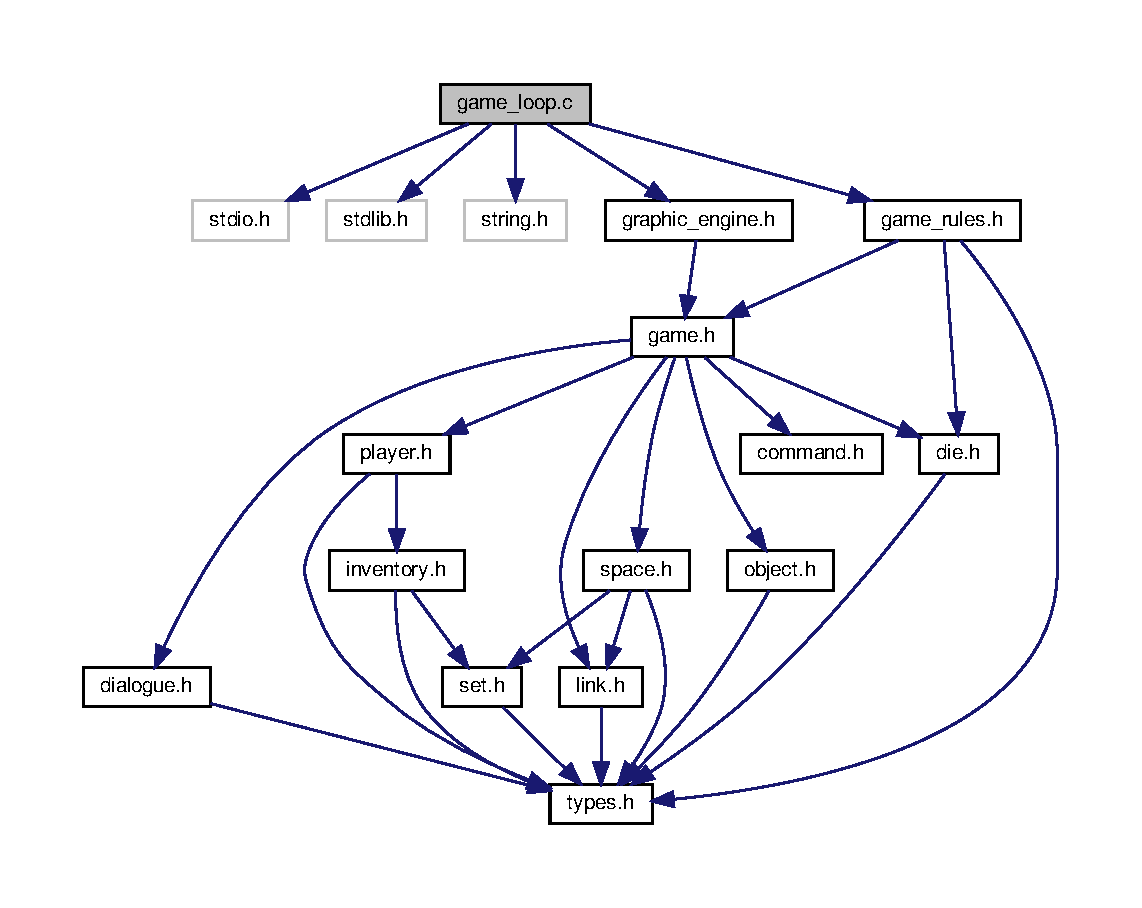
\includegraphics[width=350pt]{game__loop_8c__incl}
\end{center}
\end{figure}
\subsection*{Functions}
\begin{DoxyCompactItemize}
\item 
int \hyperlink{game__loop_8c_a0ddf1224851353fc92bfbff6f499fa97}{main} (int argc, char $\ast$argv\mbox{[}$\,$\mbox{]})
\begin{DoxyCompactList}\small\item\em main function of the game \end{DoxyCompactList}\end{DoxyCompactItemize}


\subsection{Detailed Description}
It defines the game loop, it contains the main function of the game. 

\begin{DoxyAuthor}{Author}
\end{DoxyAuthor}
\begin{DoxyVersion}{Version}
4.\+0 
\end{DoxyVersion}
\begin{DoxyDate}{Date}
12-\/02-\/2019 
\end{DoxyDate}
\begin{DoxyCopyright}{Copyright}
G\+NU Public License 
\end{DoxyCopyright}


\subsection{Function Documentation}
\mbox{\Hypertarget{game__loop_8c_a0ddf1224851353fc92bfbff6f499fa97}\label{game__loop_8c_a0ddf1224851353fc92bfbff6f499fa97}} 
\index{game\+\_\+loop.\+c@{game\+\_\+loop.\+c}!main@{main}}
\index{main@{main}!game\+\_\+loop.\+c@{game\+\_\+loop.\+c}}
\subsubsection{\texorpdfstring{main()}{main()}}
{\footnotesize\ttfamily int main (\begin{DoxyParamCaption}\item[{int}]{argc,  }\item[{char $\ast$}]{argv\mbox{[}$\,$\mbox{]} }\end{DoxyParamCaption})}



main function of the game 


\begin{DoxyParams}{Parameters}
{\em argc} & \\
\hline
{\em argv} & \\
\hline
\end{DoxyParams}
\begin{DoxyReturn}{Returns}
number 
\end{DoxyReturn}


\hypertarget{game__rules_8c}{}\section{game\+\_\+rules.\+c File Reference}
\label{game__rules_8c}\index{game\+\_\+rules.\+c@{game\+\_\+rules.\+c}}


Game Rules Module.  


{\ttfamily \#include $<$stdio.\+h$>$}\newline
{\ttfamily \#include $<$stdlib.\+h$>$}\newline
{\ttfamily \#include $<$string.\+h$>$}\newline
{\ttfamily \#include \char`\"{}game\+\_\+rules.\+h\char`\"{}}\newline
Include dependency graph for game\+\_\+rules.\+c\+:
\nopagebreak
\begin{figure}[H]
\begin{center}
\leavevmode
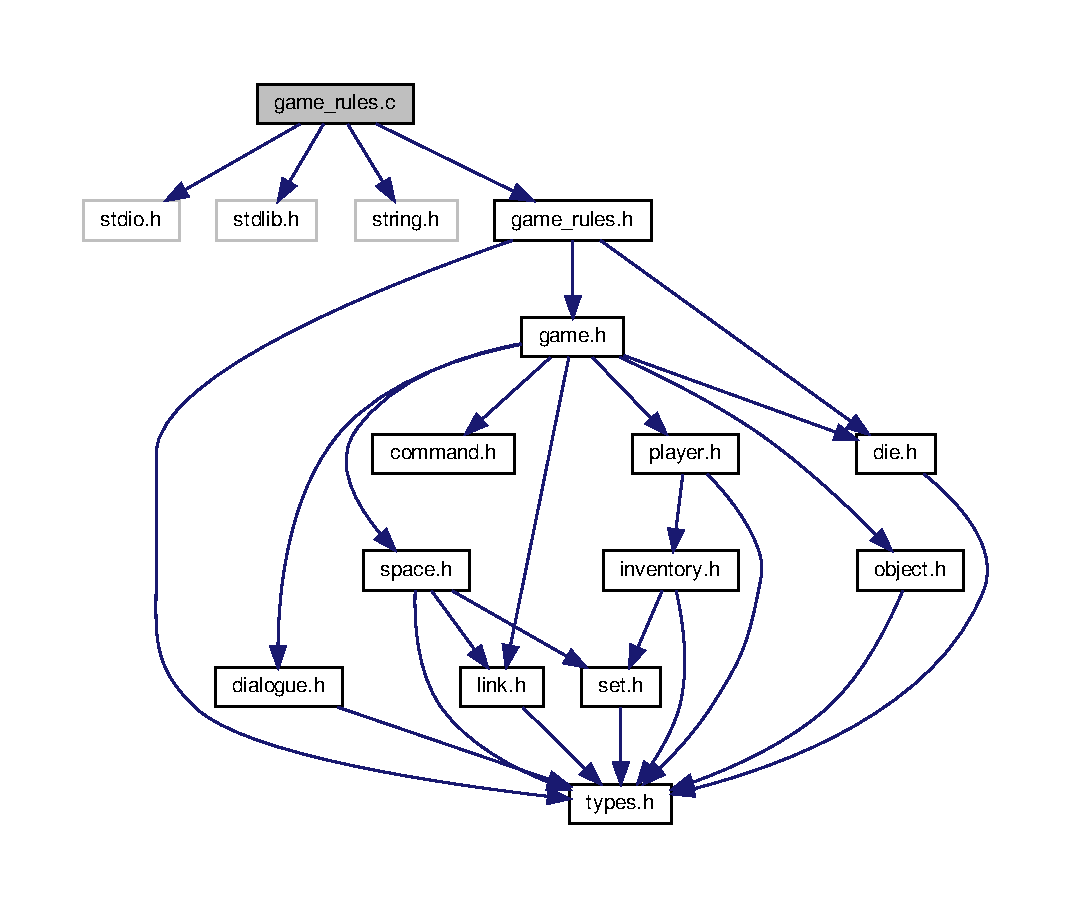
\includegraphics[width=350pt]{game__rules_8c__incl}
\end{center}
\end{figure}
\subsection*{Data Structures}
\begin{DoxyCompactItemize}
\item 
struct \hyperlink{struct__Rules}{\+\_\+\+Rules}
\begin{DoxyCompactList}\small\item\em defines the rules structure \end{DoxyCompactList}\end{DoxyCompactItemize}
\subsection*{Macros}
\begin{DoxyCompactItemize}
\item 
\mbox{\Hypertarget{game__rules_8c_a4ffabc057b1fee7abd6a3555b03320dd}\label{game__rules_8c_a4ffabc057b1fee7abd6a3555b03320dd}} 
\#define \hyperlink{game__rules_8c_a4ffabc057b1fee7abd6a3555b03320dd}{N\+\_\+\+R\+U\+L\+ES}~6
\begin{DoxyCompactList}\small\item\em defines the macro for the number of rules \end{DoxyCompactList}\item 
\mbox{\Hypertarget{game__rules_8c_a128a0e8baeaa0cf0f82b55544f40f494}\label{game__rules_8c_a128a0e8baeaa0cf0f82b55544f40f494}} 
\#define \hyperlink{game__rules_8c_a128a0e8baeaa0cf0f82b55544f40f494}{N\+\_\+\+S\+P\+A\+C\+ES}~20
\begin{DoxyCompactList}\small\item\em defines the macro for the number of spaces \end{DoxyCompactList}\end{DoxyCompactItemize}
\subsection*{Typedefs}
\begin{DoxyCompactItemize}
\item 
\mbox{\Hypertarget{game__rules_8c_a7c23e7b371062725f3d823c54d975eae}\label{game__rules_8c_a7c23e7b371062725f3d823c54d975eae}} 
typedef void($\ast$ \hyperlink{game__rules_8c_a7c23e7b371062725f3d823c54d975eae}{callback\+\_\+fn}) (\hyperlink{game__rules_8h_add6e93d3be9e55f9ff3b469e3d24cf13}{Rules} $\ast$rules)
\begin{DoxyCompactList}\small\item\em defines callbacks \end{DoxyCompactList}\end{DoxyCompactItemize}
\subsection*{Functions}
\begin{DoxyCompactItemize}
\item 
void \hyperlink{game__rules_8c_a0775ffa7b0e38f0d48349413a1dcb9e9}{rules\+\_\+callback\+\_\+\+R0} (\hyperlink{game__rules_8h_add6e93d3be9e55f9ff3b469e3d24cf13}{Rules} $\ast$game\+Rules)
\begin{DoxyCompactList}\small\item\em callback for R0 \end{DoxyCompactList}\item 
void \hyperlink{game__rules_8c_a9f639fea17a6adcd59c71715c9271e37}{rules\+\_\+callback\+\_\+\+R1} (\hyperlink{game__rules_8h_add6e93d3be9e55f9ff3b469e3d24cf13}{Rules} $\ast$rules)
\begin{DoxyCompactList}\small\item\em callback for R1 \end{DoxyCompactList}\item 
void \hyperlink{game__rules_8c_a4444290fa5f5e159cfe2848a0713beff}{rules\+\_\+callback\+\_\+\+R2} (\hyperlink{game__rules_8h_add6e93d3be9e55f9ff3b469e3d24cf13}{Rules} $\ast$rules)
\begin{DoxyCompactList}\small\item\em callback for R2 \end{DoxyCompactList}\item 
void \hyperlink{game__rules_8c_a93b10462610835ed3cbb7519fb1a795c}{rules\+\_\+callback\+\_\+\+R3} (\hyperlink{game__rules_8h_add6e93d3be9e55f9ff3b469e3d24cf13}{Rules} $\ast$rules)
\begin{DoxyCompactList}\small\item\em callback for R3 \end{DoxyCompactList}\item 
void \hyperlink{game__rules_8c_a3dd9a1f29dedcb320ff6b47f510d402c}{rules\+\_\+callback\+\_\+\+R4} (\hyperlink{game__rules_8h_add6e93d3be9e55f9ff3b469e3d24cf13}{Rules} $\ast$rules)
\begin{DoxyCompactList}\small\item\em callback for R4 \end{DoxyCompactList}\item 
void \hyperlink{game__rules_8c_a165bb3ce07391907a6e5ecd835e19305}{rules\+\_\+callback\+\_\+\+R5} (\hyperlink{game__rules_8h_add6e93d3be9e55f9ff3b469e3d24cf13}{Rules} $\ast$rules)
\begin{DoxyCompactList}\small\item\em callback for R5 \end{DoxyCompactList}\item 
\hyperlink{game__rules_8h_add6e93d3be9e55f9ff3b469e3d24cf13}{Rules} $\ast$ \hyperlink{game__rules_8c_aad961700eb0f609e599d442498b318c5}{Rules\+Create} ()
\begin{DoxyCompactList}\small\item\em create a game rule \end{DoxyCompactList}\item 
\hyperlink{types_8h_a32c27cc471df37f4fc818d65de0a56c4}{S\+T\+A\+T\+US} \hyperlink{game__rules_8c_acbd71f0908b3eb7e5ed5958d51b13cab}{Rules\+Destroy} (\hyperlink{game__rules_8h_add6e93d3be9e55f9ff3b469e3d24cf13}{Rules} $\ast$rules)
\begin{DoxyCompactList}\small\item\em destroy rule \end{DoxyCompactList}\item 
\hyperlink{types_8h_a32c27cc471df37f4fc818d65de0a56c4}{S\+T\+A\+T\+US} \hyperlink{game__rules_8c_aba5baaead34b2b6ac9c8bf5949c0c11c}{Rules\+Start} (\hyperlink{game__rules_8h_add6e93d3be9e55f9ff3b469e3d24cf13}{Rules} $\ast$rules, \hyperlink{game_8h_a57156d39c530aec3fba3a9dad8c2dc6a}{Game} $\ast$game, \hyperlink{types_8h_a3e5b8192e7d9ffaf3542f1210aec18dd}{B\+O\+OL} disable, int rule)
\begin{DoxyCompactList}\small\item\em set rules start \end{DoxyCompactList}\item 
void \hyperlink{game__rules_8c_ac657c59bd9d82e017213323a8dd4ed7c}{Random\+Rule} (\hyperlink{game__rules_8h_add6e93d3be9e55f9ff3b469e3d24cf13}{Rules} $\ast$rules)
\begin{DoxyCompactList}\small\item\em set randum rules \end{DoxyCompactList}\end{DoxyCompactItemize}


\subsection{Detailed Description}
Game Rules Module. 

\begin{DoxyAuthor}{Author}
\end{DoxyAuthor}
\begin{DoxyVersion}{Version}
1.\+0 
\end{DoxyVersion}
\begin{DoxyDate}{Date}

\end{DoxyDate}


\subsection{Function Documentation}
\mbox{\Hypertarget{game__rules_8c_ac657c59bd9d82e017213323a8dd4ed7c}\label{game__rules_8c_ac657c59bd9d82e017213323a8dd4ed7c}} 
\index{game\+\_\+rules.\+c@{game\+\_\+rules.\+c}!Random\+Rule@{Random\+Rule}}
\index{Random\+Rule@{Random\+Rule}!game\+\_\+rules.\+c@{game\+\_\+rules.\+c}}
\subsubsection{\texorpdfstring{Random\+Rule()}{RandomRule()}}
{\footnotesize\ttfamily void Random\+Rule (\begin{DoxyParamCaption}\item[{\hyperlink{game__rules_8h_add6e93d3be9e55f9ff3b469e3d24cf13}{Rules} $\ast$}]{rules }\end{DoxyParamCaption})}



set randum rules 


\begin{DoxyParams}{Parameters}
{\em rules} & \\
\hline
\end{DoxyParams}
\begin{DoxyReturn}{Returns}
void 
\end{DoxyReturn}
\mbox{\Hypertarget{game__rules_8c_a0775ffa7b0e38f0d48349413a1dcb9e9}\label{game__rules_8c_a0775ffa7b0e38f0d48349413a1dcb9e9}} 
\index{game\+\_\+rules.\+c@{game\+\_\+rules.\+c}!rules\+\_\+callback\+\_\+\+R0@{rules\+\_\+callback\+\_\+\+R0}}
\index{rules\+\_\+callback\+\_\+\+R0@{rules\+\_\+callback\+\_\+\+R0}!game\+\_\+rules.\+c@{game\+\_\+rules.\+c}}
\subsubsection{\texorpdfstring{rules\+\_\+callback\+\_\+\+R0()}{rules\_callback\_R0()}}
{\footnotesize\ttfamily void rules\+\_\+callback\+\_\+\+R0 (\begin{DoxyParamCaption}\item[{\hyperlink{game__rules_8h_add6e93d3be9e55f9ff3b469e3d24cf13}{Rules} $\ast$}]{game\+Rules }\end{DoxyParamCaption})}



callback for R0 


\begin{DoxyParams}{Parameters}
{\em game\+Rules} & \\
\hline
\end{DoxyParams}
\begin{DoxyReturn}{Returns}
void 
\end{DoxyReturn}
\mbox{\Hypertarget{game__rules_8c_a9f639fea17a6adcd59c71715c9271e37}\label{game__rules_8c_a9f639fea17a6adcd59c71715c9271e37}} 
\index{game\+\_\+rules.\+c@{game\+\_\+rules.\+c}!rules\+\_\+callback\+\_\+\+R1@{rules\+\_\+callback\+\_\+\+R1}}
\index{rules\+\_\+callback\+\_\+\+R1@{rules\+\_\+callback\+\_\+\+R1}!game\+\_\+rules.\+c@{game\+\_\+rules.\+c}}
\subsubsection{\texorpdfstring{rules\+\_\+callback\+\_\+\+R1()}{rules\_callback\_R1()}}
{\footnotesize\ttfamily void rules\+\_\+callback\+\_\+\+R1 (\begin{DoxyParamCaption}\item[{\hyperlink{game__rules_8h_add6e93d3be9e55f9ff3b469e3d24cf13}{Rules} $\ast$}]{rules }\end{DoxyParamCaption})}



callback for R1 


\begin{DoxyParams}{Parameters}
{\em rules} & \\
\hline
\end{DoxyParams}
\begin{DoxyReturn}{Returns}
void 
\end{DoxyReturn}
\mbox{\Hypertarget{game__rules_8c_a4444290fa5f5e159cfe2848a0713beff}\label{game__rules_8c_a4444290fa5f5e159cfe2848a0713beff}} 
\index{game\+\_\+rules.\+c@{game\+\_\+rules.\+c}!rules\+\_\+callback\+\_\+\+R2@{rules\+\_\+callback\+\_\+\+R2}}
\index{rules\+\_\+callback\+\_\+\+R2@{rules\+\_\+callback\+\_\+\+R2}!game\+\_\+rules.\+c@{game\+\_\+rules.\+c}}
\subsubsection{\texorpdfstring{rules\+\_\+callback\+\_\+\+R2()}{rules\_callback\_R2()}}
{\footnotesize\ttfamily void rules\+\_\+callback\+\_\+\+R2 (\begin{DoxyParamCaption}\item[{\hyperlink{game__rules_8h_add6e93d3be9e55f9ff3b469e3d24cf13}{Rules} $\ast$}]{rules }\end{DoxyParamCaption})}



callback for R2 


\begin{DoxyParams}{Parameters}
{\em rules} & \\
\hline
\end{DoxyParams}
\begin{DoxyReturn}{Returns}
void 
\end{DoxyReturn}
\mbox{\Hypertarget{game__rules_8c_a93b10462610835ed3cbb7519fb1a795c}\label{game__rules_8c_a93b10462610835ed3cbb7519fb1a795c}} 
\index{game\+\_\+rules.\+c@{game\+\_\+rules.\+c}!rules\+\_\+callback\+\_\+\+R3@{rules\+\_\+callback\+\_\+\+R3}}
\index{rules\+\_\+callback\+\_\+\+R3@{rules\+\_\+callback\+\_\+\+R3}!game\+\_\+rules.\+c@{game\+\_\+rules.\+c}}
\subsubsection{\texorpdfstring{rules\+\_\+callback\+\_\+\+R3()}{rules\_callback\_R3()}}
{\footnotesize\ttfamily void rules\+\_\+callback\+\_\+\+R3 (\begin{DoxyParamCaption}\item[{\hyperlink{game__rules_8h_add6e93d3be9e55f9ff3b469e3d24cf13}{Rules} $\ast$}]{rules }\end{DoxyParamCaption})}



callback for R3 


\begin{DoxyParams}{Parameters}
{\em rules} & \\
\hline
\end{DoxyParams}
\begin{DoxyReturn}{Returns}
void 
\end{DoxyReturn}
\mbox{\Hypertarget{game__rules_8c_a3dd9a1f29dedcb320ff6b47f510d402c}\label{game__rules_8c_a3dd9a1f29dedcb320ff6b47f510d402c}} 
\index{game\+\_\+rules.\+c@{game\+\_\+rules.\+c}!rules\+\_\+callback\+\_\+\+R4@{rules\+\_\+callback\+\_\+\+R4}}
\index{rules\+\_\+callback\+\_\+\+R4@{rules\+\_\+callback\+\_\+\+R4}!game\+\_\+rules.\+c@{game\+\_\+rules.\+c}}
\subsubsection{\texorpdfstring{rules\+\_\+callback\+\_\+\+R4()}{rules\_callback\_R4()}}
{\footnotesize\ttfamily void rules\+\_\+callback\+\_\+\+R4 (\begin{DoxyParamCaption}\item[{\hyperlink{game__rules_8h_add6e93d3be9e55f9ff3b469e3d24cf13}{Rules} $\ast$}]{rules }\end{DoxyParamCaption})}



callback for R4 


\begin{DoxyParams}{Parameters}
{\em rules} & \\
\hline
\end{DoxyParams}
\begin{DoxyReturn}{Returns}
void 
\end{DoxyReturn}
\mbox{\Hypertarget{game__rules_8c_a165bb3ce07391907a6e5ecd835e19305}\label{game__rules_8c_a165bb3ce07391907a6e5ecd835e19305}} 
\index{game\+\_\+rules.\+c@{game\+\_\+rules.\+c}!rules\+\_\+callback\+\_\+\+R5@{rules\+\_\+callback\+\_\+\+R5}}
\index{rules\+\_\+callback\+\_\+\+R5@{rules\+\_\+callback\+\_\+\+R5}!game\+\_\+rules.\+c@{game\+\_\+rules.\+c}}
\subsubsection{\texorpdfstring{rules\+\_\+callback\+\_\+\+R5()}{rules\_callback\_R5()}}
{\footnotesize\ttfamily void rules\+\_\+callback\+\_\+\+R5 (\begin{DoxyParamCaption}\item[{\hyperlink{game__rules_8h_add6e93d3be9e55f9ff3b469e3d24cf13}{Rules} $\ast$}]{rules }\end{DoxyParamCaption})}



callback for R5 


\begin{DoxyParams}{Parameters}
{\em rules} & \\
\hline
\end{DoxyParams}
\begin{DoxyReturn}{Returns}
void 
\end{DoxyReturn}
\mbox{\Hypertarget{game__rules_8c_aad961700eb0f609e599d442498b318c5}\label{game__rules_8c_aad961700eb0f609e599d442498b318c5}} 
\index{game\+\_\+rules.\+c@{game\+\_\+rules.\+c}!Rules\+Create@{Rules\+Create}}
\index{Rules\+Create@{Rules\+Create}!game\+\_\+rules.\+c@{game\+\_\+rules.\+c}}
\subsubsection{\texorpdfstring{Rules\+Create()}{RulesCreate()}}
{\footnotesize\ttfamily \hyperlink{game__rules_8h_add6e93d3be9e55f9ff3b469e3d24cf13}{Rules}$\ast$ Rules\+Create (\begin{DoxyParamCaption}{ }\end{DoxyParamCaption})}



create a game rule 

\begin{DoxyReturn}{Returns}
Rule or N\+U\+LL in case of error 
\end{DoxyReturn}
\mbox{\Hypertarget{game__rules_8c_acbd71f0908b3eb7e5ed5958d51b13cab}\label{game__rules_8c_acbd71f0908b3eb7e5ed5958d51b13cab}} 
\index{game\+\_\+rules.\+c@{game\+\_\+rules.\+c}!Rules\+Destroy@{Rules\+Destroy}}
\index{Rules\+Destroy@{Rules\+Destroy}!game\+\_\+rules.\+c@{game\+\_\+rules.\+c}}
\subsubsection{\texorpdfstring{Rules\+Destroy()}{RulesDestroy()}}
{\footnotesize\ttfamily \hyperlink{types_8h_a32c27cc471df37f4fc818d65de0a56c4}{S\+T\+A\+T\+US} Rules\+Destroy (\begin{DoxyParamCaption}\item[{\hyperlink{game__rules_8h_add6e93d3be9e55f9ff3b469e3d24cf13}{Rules} $\ast$}]{rules }\end{DoxyParamCaption})}



destroy rule 


\begin{DoxyParams}{Parameters}
{\em rules} & \\
\hline
\end{DoxyParams}
\begin{DoxyReturn}{Returns}
OK, or E\+R\+R\+OR 
\end{DoxyReturn}
\mbox{\Hypertarget{game__rules_8c_aba5baaead34b2b6ac9c8bf5949c0c11c}\label{game__rules_8c_aba5baaead34b2b6ac9c8bf5949c0c11c}} 
\index{game\+\_\+rules.\+c@{game\+\_\+rules.\+c}!Rules\+Start@{Rules\+Start}}
\index{Rules\+Start@{Rules\+Start}!game\+\_\+rules.\+c@{game\+\_\+rules.\+c}}
\subsubsection{\texorpdfstring{Rules\+Start()}{RulesStart()}}
{\footnotesize\ttfamily \hyperlink{types_8h_a32c27cc471df37f4fc818d65de0a56c4}{S\+T\+A\+T\+US} Rules\+Start (\begin{DoxyParamCaption}\item[{\hyperlink{game__rules_8h_add6e93d3be9e55f9ff3b469e3d24cf13}{Rules} $\ast$}]{rules,  }\item[{\hyperlink{game_8h_a57156d39c530aec3fba3a9dad8c2dc6a}{Game} $\ast$}]{game,  }\item[{\hyperlink{types_8h_a3e5b8192e7d9ffaf3542f1210aec18dd}{B\+O\+OL}}]{disable,  }\item[{int}]{rule }\end{DoxyParamCaption})}



set rules start 


\begin{DoxyParams}{Parameters}
{\em rules} & \\
\hline
{\em game} & \\
\hline
{\em disable} & \\
\hline
{\em rule} & \\
\hline
\end{DoxyParams}
\begin{DoxyReturn}{Returns}
OK or E\+R\+R\+OR 
\end{DoxyReturn}


\hypertarget{game__rules_8h}{\section{include/game\+\_\+rules.h File Reference}
\label{game__rules_8h}\index{include/game\+\_\+rules.\+h@{include/game\+\_\+rules.\+h}}
}


It defines the game rules interface.  


{\ttfamily \#include \char`\"{}../include/types.\+h\char`\"{}}\\*
{\ttfamily \#include \char`\"{}../include/game.\+h\char`\"{}}\\*
Include dependency graph for game\+\_\+rules.\+h\+:
\nopagebreak
\begin{figure}[H]
\begin{center}
\leavevmode
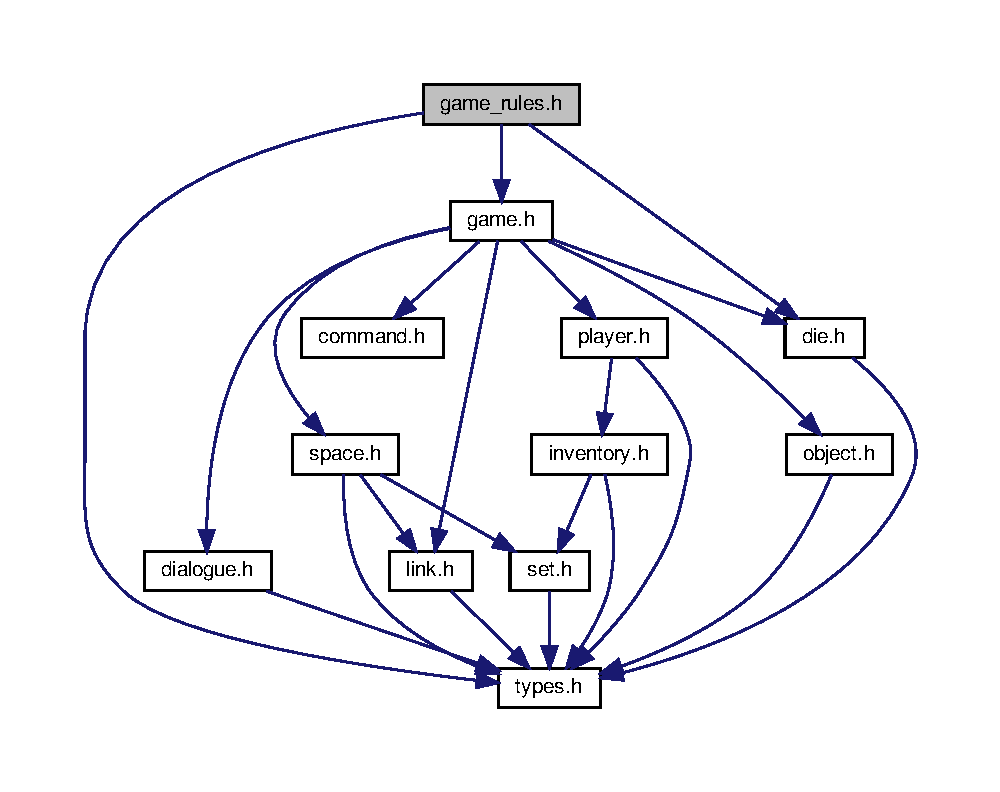
\includegraphics[width=350pt]{game__rules_8h__incl}
\end{center}
\end{figure}
This graph shows which files directly or indirectly include this file\+:
\nopagebreak
\begin{figure}[H]
\begin{center}
\leavevmode
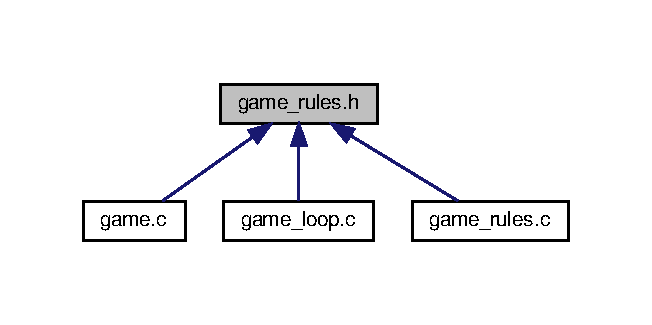
\includegraphics[width=279pt]{game__rules_8h__dep__incl}
\end{center}
\end{figure}
\subsection*{Typedefs}
\begin{DoxyCompactItemize}
\item 
\hypertarget{game__rules_8h_a60dd8c87b598cf179dc700a896badc6c}{typedef enum \hyperlink{game__rules_8h_af65db71933f393ce1a8b0c0269987bd4}{enum\+\_\+\+Rules} \hyperlink{game__rules_8h_a60dd8c87b598cf179dc700a896badc6c}{T\+\_\+\+Rule}}\label{game__rules_8h_a60dd8c87b598cf179dc700a896badc6c}

\begin{DoxyCompactList}\small\item\em Lista de posibles reglas. \end{DoxyCompactList}\item 
\hypertarget{game__rules_8h_a427dee1046e87ecb0d82e194918d0c4b}{typedef struct \hyperlink{struct__GameRules}{\+\_\+\+Game\+Rules} \hyperlink{game__rules_8h_a427dee1046e87ecb0d82e194918d0c4b}{Game\+Rules}}\label{game__rules_8h_a427dee1046e87ecb0d82e194918d0c4b}

\begin{DoxyCompactList}\small\item\em Estructura del game\+Rules. \end{DoxyCompactList}\end{DoxyCompactItemize}
\subsection*{Enumerations}
\begin{DoxyCompactItemize}
\item 
\hypertarget{game__rules_8h_af65db71933f393ce1a8b0c0269987bd4}{enum \hyperlink{game__rules_8h_af65db71933f393ce1a8b0c0269987bd4}{enum\+\_\+\+Rules} \{ \\*
{\bfseries N\+O\+\_\+\+R\+U\+L\+E} = -\/1, 
{\bfseries O\+C\+U\+L\+T}, 
{\bfseries O\+F\+F}, 
{\bfseries O\+N}, 
\\*
{\bfseries C\+L\+O\+S\+E}, 
{\bfseries S\+H\+O\+W}, 
{\bfseries C\+H\+A\+N\+G\+E}, 
{\bfseries E\+L\+I\+M\+I\+N\+A\+T\+E}, 
\\*
{\bfseries R\+E\+G\+E\+N\+E\+R\+A\+T\+E}, 
{\bfseries N\+E\+W\+E\+X\+I\+T}
 \}}\label{game__rules_8h_af65db71933f393ce1a8b0c0269987bd4}

\begin{DoxyCompactList}\small\item\em Lista de posibles reglas. \end{DoxyCompactList}\end{DoxyCompactItemize}
\subsection*{Functions}
\begin{DoxyCompactItemize}
\item 
\hyperlink{game__rules_8h_a427dee1046e87ecb0d82e194918d0c4b}{Game\+Rules} $\ast$ \hyperlink{game__rules_8h_aefc0992f9d3b8228ea705408b535ca5c}{game\+\_\+rules\+\_\+create} ()
\begin{DoxyCompactList}\small\item\em Funcion para reservar memoria para el modulo de las reglas. \end{DoxyCompactList}\item 
\hyperlink{types_8h_a32c27cc471df37f4fc818d65de0a56c4}{S\+T\+A\+T\+U\+S} \hyperlink{game__rules_8h_aeae24b9ec0c75216361ba2363c19847b}{game\+\_\+rules\+\_\+destroy} (\hyperlink{game__rules_8h_a427dee1046e87ecb0d82e194918d0c4b}{Game\+Rules} $\ast$game\+Rules)
\begin{DoxyCompactList}\small\item\em Funcion que libera memoria. \end{DoxyCompactList}\item 
\hyperlink{types_8h_a32c27cc471df37f4fc818d65de0a56c4}{S\+T\+A\+T\+U\+S} \hyperlink{game__rules_8h_a84316ec7ab939c928c9a702ba571f90e}{game\+\_\+rules\+\_\+play} (\hyperlink{game__rules_8h_a427dee1046e87ecb0d82e194918d0c4b}{Game\+Rules} $\ast$game\+Rules, \hyperlink{game_8h_a57156d39c530aec3fba3a9dad8c2dc6a}{Game} $\ast$game, \hyperlink{types_8h_a3e5b8192e7d9ffaf3542f1210aec18dd}{B\+O\+O\+L} no\+\_\+rules)
\begin{DoxyCompactList}\small\item\em Funcion para jugar. \end{DoxyCompactList}\end{DoxyCompactItemize}


\subsection{Detailed Description}
It defines the game rules interface. 

\begin{DoxyAuthor}{Author}
Julia Simon 
\end{DoxyAuthor}
\begin{DoxyVersion}{Version}
1.\+0 
\end{DoxyVersion}
\begin{DoxyDate}{Date}
02/05/2018 
\end{DoxyDate}


\subsection{Function Documentation}
\hypertarget{game__rules_8h_aefc0992f9d3b8228ea705408b535ca5c}{\index{game\+\_\+rules.\+h@{game\+\_\+rules.\+h}!game\+\_\+rules\+\_\+create@{game\+\_\+rules\+\_\+create}}
\index{game\+\_\+rules\+\_\+create@{game\+\_\+rules\+\_\+create}!game\+\_\+rules.\+h@{game\+\_\+rules.\+h}}
\subsubsection[{game\+\_\+rules\+\_\+create}]{\setlength{\rightskip}{0pt plus 5cm}{\bf Game\+Rules}$\ast$ game\+\_\+rules\+\_\+create (
\begin{DoxyParamCaption}
{}
\end{DoxyParamCaption}
)}}\label{game__rules_8h_aefc0992f9d3b8228ea705408b535ca5c}


Funcion para reservar memoria para el modulo de las reglas. 

\begin{DoxyAuthor}{Author}
Julia Simon 
\end{DoxyAuthor}
\begin{DoxyReturn}{Returns}
puntero al modulo 
\end{DoxyReturn}
\hypertarget{game__rules_8h_aeae24b9ec0c75216361ba2363c19847b}{\index{game\+\_\+rules.\+h@{game\+\_\+rules.\+h}!game\+\_\+rules\+\_\+destroy@{game\+\_\+rules\+\_\+destroy}}
\index{game\+\_\+rules\+\_\+destroy@{game\+\_\+rules\+\_\+destroy}!game\+\_\+rules.\+h@{game\+\_\+rules.\+h}}
\subsubsection[{game\+\_\+rules\+\_\+destroy}]{\setlength{\rightskip}{0pt plus 5cm}{\bf S\+T\+A\+T\+U\+S} game\+\_\+rules\+\_\+destroy (
\begin{DoxyParamCaption}
\item[{{\bf Game\+Rules} $\ast$}]{game\+Rules}
\end{DoxyParamCaption}
)}}\label{game__rules_8h_aeae24b9ec0c75216361ba2363c19847b}


Funcion que libera memoria. 

\begin{DoxyAuthor}{Author}
Julia Simon 
\end{DoxyAuthor}

\begin{DoxyParams}{Parameters}
{\em game\+Rules} & modulo a destruir \\
\hline
\end{DoxyParams}
\begin{DoxyReturn}{Returns}
Ok O E\+R\+R\+O\+R si se libera bien o no 
\end{DoxyReturn}
\hypertarget{game__rules_8h_a84316ec7ab939c928c9a702ba571f90e}{\index{game\+\_\+rules.\+h@{game\+\_\+rules.\+h}!game\+\_\+rules\+\_\+play@{game\+\_\+rules\+\_\+play}}
\index{game\+\_\+rules\+\_\+play@{game\+\_\+rules\+\_\+play}!game\+\_\+rules.\+h@{game\+\_\+rules.\+h}}
\subsubsection[{game\+\_\+rules\+\_\+play}]{\setlength{\rightskip}{0pt plus 5cm}{\bf S\+T\+A\+T\+U\+S} game\+\_\+rules\+\_\+play (
\begin{DoxyParamCaption}
\item[{{\bf Game\+Rules} $\ast$}]{game\+Rules, }
\item[{{\bf Game} $\ast$}]{game, }
\item[{{\bf B\+O\+O\+L}}]{no\+\_\+rules}
\end{DoxyParamCaption}
)}}\label{game__rules_8h_a84316ec7ab939c928c9a702ba571f90e}


Funcion para jugar. 

\begin{DoxyAuthor}{Author}
Julia S\+Imon 
\end{DoxyAuthor}

\begin{DoxyParams}{Parameters}
{\em game\+Rules} & modulo de reglas \\
\hline
{\em game} & juego \\
\hline
{\em no\+\_\+rules} & para indicar que queremos jugar sin reglas \\
\hline
\end{DoxyParams}
\begin{DoxyReturn}{Returns}
Ok O E\+R\+R\+O\+R si se libera bien o no 
\end{DoxyReturn}

\hypertarget{gamemanagement_8c}{}\section{gamemanagement.\+c File Reference}
\label{gamemanagement_8c}\index{gamemanagement.\+c@{gamemanagement.\+c}}


It defines the module of gamemanagement, contains different function of game, link,space.  


{\ttfamily \#include $<$stdio.\+h$>$}\newline
{\ttfamily \#include $<$stdlib.\+h$>$}\newline
{\ttfamily \#include $<$string.\+h$>$}\newline
{\ttfamily \#include \char`\"{}gamemanagement.\+h\char`\"{}}\newline
Include dependency graph for gamemanagement.\+c\+:
\nopagebreak
\begin{figure}[H]
\begin{center}
\leavevmode
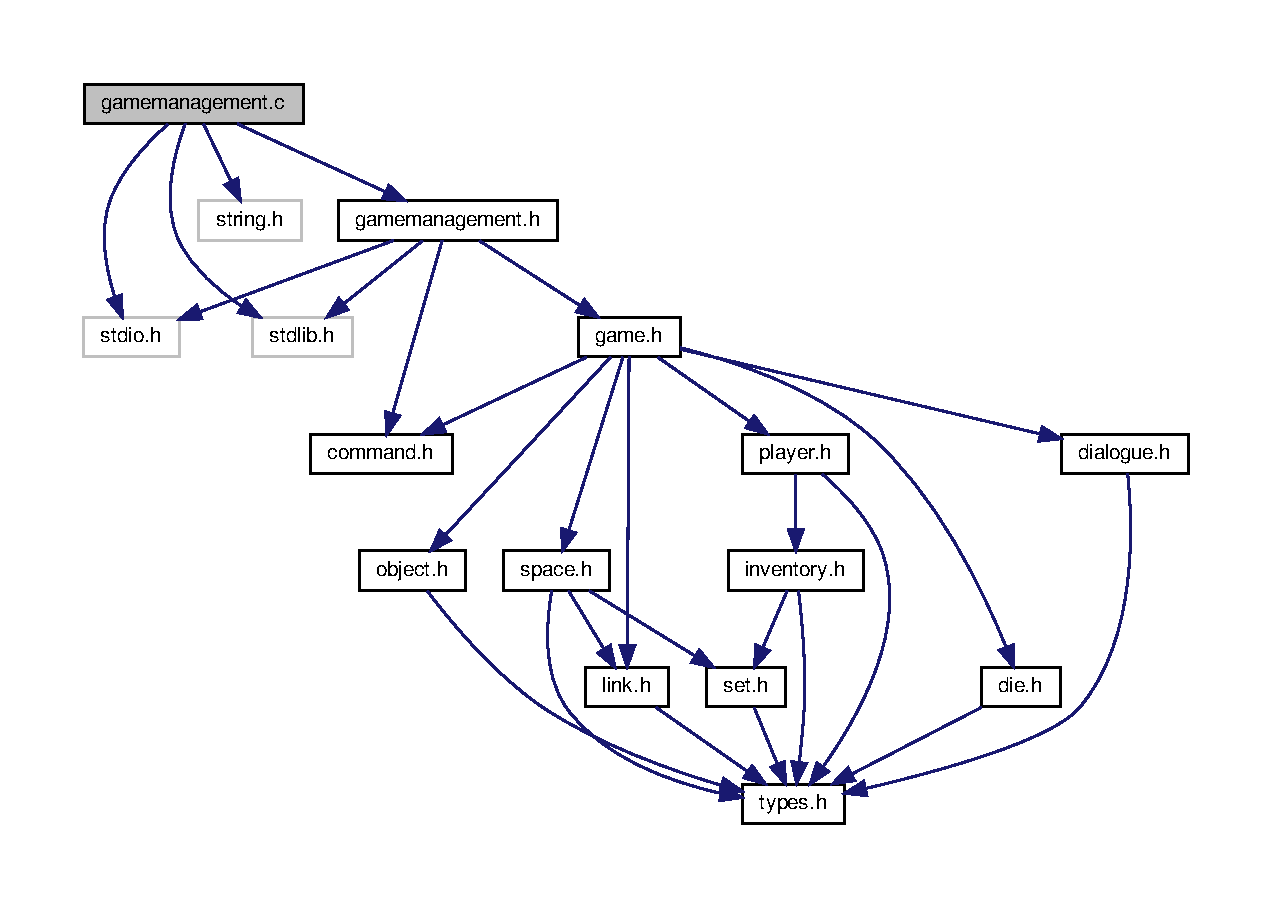
\includegraphics[width=350pt]{gamemanagement_8c__incl}
\end{center}
\end{figure}
\subsection*{Functions}
\begin{DoxyCompactItemize}
\item 
\hyperlink{types_8h_a32c27cc471df37f4fc818d65de0a56c4}{S\+T\+A\+T\+US} \hyperlink{gamemanagement_8c_ae5ad86de0a92d9eccb234948458da7f1}{game\+\_\+add\+\_\+space} (\hyperlink{game_8h_a57156d39c530aec3fba3a9dad8c2dc6a}{Game} $\ast$game, \hyperlink{space_8h_a67533ffc2b70463baecc38fb0629bbfc}{Space} $\ast$space)
\item 
\hyperlink{types_8h_a32c27cc471df37f4fc818d65de0a56c4}{S\+T\+A\+T\+US} \hyperlink{gamemanagement_8c_a0d01072a28b01545d36240cb8bd9d4f8}{game\+\_\+load\+\_\+spaces} (\hyperlink{game_8h_a57156d39c530aec3fba3a9dad8c2dc6a}{Game} $\ast$game, char $\ast$filename)
\begin{DoxyCompactList}\small\item\em load spaces \end{DoxyCompactList}\item 
\hyperlink{types_8h_a32c27cc471df37f4fc818d65de0a56c4}{S\+T\+A\+T\+US} \hyperlink{gamemanagement_8c_a66279ceefe2efe0967be248e8d0e0565}{game\+\_\+load\+\_\+objects} (\hyperlink{game_8h_a57156d39c530aec3fba3a9dad8c2dc6a}{Game} $\ast$game, char $\ast$filename)
\begin{DoxyCompactList}\small\item\em it load the objects to the game to be able to play \end{DoxyCompactList}\item 
\hyperlink{types_8h_a32c27cc471df37f4fc818d65de0a56c4}{S\+T\+A\+T\+US} \hyperlink{gamemanagement_8c_a9597a8e456aa74db536e87d56f56c3b4}{game\+\_\+add\+\_\+object} (\hyperlink{game_8h_a57156d39c530aec3fba3a9dad8c2dc6a}{Game} $\ast$game, \hyperlink{object_8h_a7f8bbcda919b65ce67f92fba08e0212f}{Object} $\ast$object)
\begin{DoxyCompactList}\small\item\em add an object to the game \end{DoxyCompactList}\item 
\hyperlink{types_8h_a32c27cc471df37f4fc818d65de0a56c4}{S\+T\+A\+T\+US} \hyperlink{gamemanagement_8c_a4691bee17d5784ad6eb257dfbb252c27}{game\+\_\+add\+\_\+link} (\hyperlink{game_8h_a57156d39c530aec3fba3a9dad8c2dc6a}{Game} $\ast$game, \hyperlink{link_8h_ae3b299941e67be6971bfd64a25505eff}{Link} $\ast$link)
\begin{DoxyCompactList}\small\item\em add links \end{DoxyCompactList}\item 
\hyperlink{types_8h_a32c27cc471df37f4fc818d65de0a56c4}{S\+T\+A\+T\+US} \hyperlink{gamemanagement_8c_aab4103cf97109ac921f358858ca2684d}{game\+\_\+load\+\_\+links} (\hyperlink{game_8h_a57156d39c530aec3fba3a9dad8c2dc6a}{Game} $\ast$game, char $\ast$filename)
\begin{DoxyCompactList}\small\item\em it load the links to the game to be able to play \end{DoxyCompactList}\item 
\hyperlink{types_8h_a32c27cc471df37f4fc818d65de0a56c4}{S\+T\+A\+T\+US} \hyperlink{gamemanagement_8c_aa5c75aee9b0f84a7f3e194de25714df4}{gamemanagement\+\_\+save} (\hyperlink{game_8h_a57156d39c530aec3fba3a9dad8c2dc6a}{Game} $\ast$game, const char $\ast$dir)
\begin{DoxyCompactList}\small\item\em it saves the game \end{DoxyCompactList}\item 
\hyperlink{types_8h_a32c27cc471df37f4fc818d65de0a56c4}{S\+T\+A\+T\+US} \hyperlink{gamemanagement_8c_a6a7a09a84b7f206004e32985bba02af6}{gamemanagement\+\_\+load} (\hyperlink{game_8h_a57156d39c530aec3fba3a9dad8c2dc6a}{Game} $\ast$game, const char $\ast$dir)
\begin{DoxyCompactList}\small\item\em it loads the game \end{DoxyCompactList}\end{DoxyCompactItemize}


\subsection{Detailed Description}
It defines the module of gamemanagement, contains different function of game, link,space. 

\begin{DoxyAuthor}{Author}
\end{DoxyAuthor}
\begin{DoxyVersion}{Version}
2.\+0 
\end{DoxyVersion}
\begin{DoxyDate}{Date}
21-\/02-\/2019 
\end{DoxyDate}
\begin{DoxyCopyright}{Copyright}
G\+NU Public License 
\end{DoxyCopyright}


\subsection{Function Documentation}
\mbox{\Hypertarget{gamemanagement_8c_a4691bee17d5784ad6eb257dfbb252c27}\label{gamemanagement_8c_a4691bee17d5784ad6eb257dfbb252c27}} 
\index{gamemanagement.\+c@{gamemanagement.\+c}!game\+\_\+add\+\_\+link@{game\+\_\+add\+\_\+link}}
\index{game\+\_\+add\+\_\+link@{game\+\_\+add\+\_\+link}!gamemanagement.\+c@{gamemanagement.\+c}}
\subsubsection{\texorpdfstring{game\+\_\+add\+\_\+link()}{game\_add\_link()}}
{\footnotesize\ttfamily \hyperlink{types_8h_a32c27cc471df37f4fc818d65de0a56c4}{S\+T\+A\+T\+US} game\+\_\+add\+\_\+link (\begin{DoxyParamCaption}\item[{\hyperlink{game_8h_a57156d39c530aec3fba3a9dad8c2dc6a}{Game} $\ast$}]{game,  }\item[{\hyperlink{link_8h_ae3b299941e67be6971bfd64a25505eff}{Link} $\ast$}]{link }\end{DoxyParamCaption})}



add links 


\begin{DoxyParams}{Parameters}
{\em game} & \\
\hline
{\em link} & \\
\hline
\end{DoxyParams}
\begin{DoxyReturn}{Returns}
OK or E\+R\+R\+OR 
\end{DoxyReturn}
\mbox{\Hypertarget{gamemanagement_8c_a9597a8e456aa74db536e87d56f56c3b4}\label{gamemanagement_8c_a9597a8e456aa74db536e87d56f56c3b4}} 
\index{gamemanagement.\+c@{gamemanagement.\+c}!game\+\_\+add\+\_\+object@{game\+\_\+add\+\_\+object}}
\index{game\+\_\+add\+\_\+object@{game\+\_\+add\+\_\+object}!gamemanagement.\+c@{gamemanagement.\+c}}
\subsubsection{\texorpdfstring{game\+\_\+add\+\_\+object()}{game\_add\_object()}}
{\footnotesize\ttfamily \hyperlink{types_8h_a32c27cc471df37f4fc818d65de0a56c4}{S\+T\+A\+T\+US} game\+\_\+add\+\_\+object (\begin{DoxyParamCaption}\item[{\hyperlink{game_8h_a57156d39c530aec3fba3a9dad8c2dc6a}{Game} $\ast$}]{game,  }\item[{\hyperlink{object_8h_a7f8bbcda919b65ce67f92fba08e0212f}{Object} $\ast$}]{object }\end{DoxyParamCaption})}



add an object to the game 


\begin{DoxyParams}{Parameters}
{\em game} & \\
\hline
{\em object} & \\
\hline
\end{DoxyParams}
\begin{DoxyReturn}{Returns}
OK, or E\+R\+R\+OR 
\end{DoxyReturn}
\mbox{\Hypertarget{gamemanagement_8c_ae5ad86de0a92d9eccb234948458da7f1}\label{gamemanagement_8c_ae5ad86de0a92d9eccb234948458da7f1}} 
\index{gamemanagement.\+c@{gamemanagement.\+c}!game\+\_\+add\+\_\+space@{game\+\_\+add\+\_\+space}}
\index{game\+\_\+add\+\_\+space@{game\+\_\+add\+\_\+space}!gamemanagement.\+c@{gamemanagement.\+c}}
\subsubsection{\texorpdfstring{game\+\_\+add\+\_\+space()}{game\_add\_space()}}
{\footnotesize\ttfamily \hyperlink{types_8h_a32c27cc471df37f4fc818d65de0a56c4}{S\+T\+A\+T\+US} game\+\_\+add\+\_\+space (\begin{DoxyParamCaption}\item[{\hyperlink{game_8h_a57156d39c530aec3fba3a9dad8c2dc6a}{Game} $\ast$}]{game,  }\item[{\hyperlink{space_8h_a67533ffc2b70463baecc38fb0629bbfc}{Space} $\ast$}]{space }\end{DoxyParamCaption})}

Private functions \mbox{\Hypertarget{gamemanagement_8c_aab4103cf97109ac921f358858ca2684d}\label{gamemanagement_8c_aab4103cf97109ac921f358858ca2684d}} 
\index{gamemanagement.\+c@{gamemanagement.\+c}!game\+\_\+load\+\_\+links@{game\+\_\+load\+\_\+links}}
\index{game\+\_\+load\+\_\+links@{game\+\_\+load\+\_\+links}!gamemanagement.\+c@{gamemanagement.\+c}}
\subsubsection{\texorpdfstring{game\+\_\+load\+\_\+links()}{game\_load\_links()}}
{\footnotesize\ttfamily \hyperlink{types_8h_a32c27cc471df37f4fc818d65de0a56c4}{S\+T\+A\+T\+US} game\+\_\+load\+\_\+links (\begin{DoxyParamCaption}\item[{\hyperlink{game_8h_a57156d39c530aec3fba3a9dad8c2dc6a}{Game} $\ast$}]{game,  }\item[{char $\ast$}]{filename }\end{DoxyParamCaption})}



it load the links to the game to be able to play 


\begin{DoxyParams}{Parameters}
{\em game} & \\
\hline
{\em filename} & \\
\hline
\end{DoxyParams}
\begin{DoxyReturn}{Returns}
OK, or E\+R\+R\+OR 
\end{DoxyReturn}
\mbox{\Hypertarget{gamemanagement_8c_a66279ceefe2efe0967be248e8d0e0565}\label{gamemanagement_8c_a66279ceefe2efe0967be248e8d0e0565}} 
\index{gamemanagement.\+c@{gamemanagement.\+c}!game\+\_\+load\+\_\+objects@{game\+\_\+load\+\_\+objects}}
\index{game\+\_\+load\+\_\+objects@{game\+\_\+load\+\_\+objects}!gamemanagement.\+c@{gamemanagement.\+c}}
\subsubsection{\texorpdfstring{game\+\_\+load\+\_\+objects()}{game\_load\_objects()}}
{\footnotesize\ttfamily \hyperlink{types_8h_a32c27cc471df37f4fc818d65de0a56c4}{S\+T\+A\+T\+US} game\+\_\+load\+\_\+objects (\begin{DoxyParamCaption}\item[{\hyperlink{game_8h_a57156d39c530aec3fba3a9dad8c2dc6a}{Game} $\ast$}]{game,  }\item[{char $\ast$}]{filename }\end{DoxyParamCaption})}



it load the objects to the game to be able to play 


\begin{DoxyParams}{Parameters}
{\em game} & \\
\hline
{\em filename} & \\
\hline
\end{DoxyParams}
\begin{DoxyReturn}{Returns}
OK, or E\+R\+R\+OR 
\end{DoxyReturn}
\mbox{\Hypertarget{gamemanagement_8c_a0d01072a28b01545d36240cb8bd9d4f8}\label{gamemanagement_8c_a0d01072a28b01545d36240cb8bd9d4f8}} 
\index{gamemanagement.\+c@{gamemanagement.\+c}!game\+\_\+load\+\_\+spaces@{game\+\_\+load\+\_\+spaces}}
\index{game\+\_\+load\+\_\+spaces@{game\+\_\+load\+\_\+spaces}!gamemanagement.\+c@{gamemanagement.\+c}}
\subsubsection{\texorpdfstring{game\+\_\+load\+\_\+spaces()}{game\_load\_spaces()}}
{\footnotesize\ttfamily \hyperlink{types_8h_a32c27cc471df37f4fc818d65de0a56c4}{S\+T\+A\+T\+US} game\+\_\+load\+\_\+spaces (\begin{DoxyParamCaption}\item[{\hyperlink{game_8h_a57156d39c530aec3fba3a9dad8c2dc6a}{Game} $\ast$}]{game,  }\item[{char $\ast$}]{filename }\end{DoxyParamCaption})}



load spaces 

it load the spaces to the game to be able to play

Private functions 
\begin{DoxyParams}{Parameters}
{\em game} & \\
\hline
{\em filename} & \\
\hline
\end{DoxyParams}
\begin{DoxyReturn}{Returns}
OK or E\+R\+R\+OR 
\end{DoxyReturn}
\mbox{\Hypertarget{gamemanagement_8c_a6a7a09a84b7f206004e32985bba02af6}\label{gamemanagement_8c_a6a7a09a84b7f206004e32985bba02af6}} 
\index{gamemanagement.\+c@{gamemanagement.\+c}!gamemanagement\+\_\+load@{gamemanagement\+\_\+load}}
\index{gamemanagement\+\_\+load@{gamemanagement\+\_\+load}!gamemanagement.\+c@{gamemanagement.\+c}}
\subsubsection{\texorpdfstring{gamemanagement\+\_\+load()}{gamemanagement\_load()}}
{\footnotesize\ttfamily \hyperlink{types_8h_a32c27cc471df37f4fc818d65de0a56c4}{S\+T\+A\+T\+US} gamemanagement\+\_\+load (\begin{DoxyParamCaption}\item[{\hyperlink{game_8h_a57156d39c530aec3fba3a9dad8c2dc6a}{Game} $\ast$}]{game,  }\item[{const char $\ast$}]{dir }\end{DoxyParamCaption})}



it loads the game 


\begin{DoxyParams}{Parameters}
{\em game} & \\
\hline
{\em dir} & \\
\hline
\end{DoxyParams}
\begin{DoxyReturn}{Returns}
OK, or E\+R\+R\+OR 
\end{DoxyReturn}
\mbox{\Hypertarget{gamemanagement_8c_aa5c75aee9b0f84a7f3e194de25714df4}\label{gamemanagement_8c_aa5c75aee9b0f84a7f3e194de25714df4}} 
\index{gamemanagement.\+c@{gamemanagement.\+c}!gamemanagement\+\_\+save@{gamemanagement\+\_\+save}}
\index{gamemanagement\+\_\+save@{gamemanagement\+\_\+save}!gamemanagement.\+c@{gamemanagement.\+c}}
\subsubsection{\texorpdfstring{gamemanagement\+\_\+save()}{gamemanagement\_save()}}
{\footnotesize\ttfamily \hyperlink{types_8h_a32c27cc471df37f4fc818d65de0a56c4}{S\+T\+A\+T\+US} gamemanagement\+\_\+save (\begin{DoxyParamCaption}\item[{\hyperlink{game_8h_a57156d39c530aec3fba3a9dad8c2dc6a}{Game} $\ast$}]{game,  }\item[{const char $\ast$}]{dir }\end{DoxyParamCaption})}



it saves the game 


\begin{DoxyParams}{Parameters}
{\em game} & \\
\hline
{\em dir} & \\
\hline
\end{DoxyParams}
\begin{DoxyReturn}{Returns}
OK, or E\+R\+R\+OR 
\end{DoxyReturn}


\hypertarget{gamemanagement_8h}{}\section{gamemanagement.\+h File Reference}
\label{gamemanagement_8h}\index{gamemanagement.\+h@{gamemanagement.\+h}}


It defines the header of gamemanagement.  


{\ttfamily \#include $<$stdio.\+h$>$}\newline
{\ttfamily \#include $<$stdlib.\+h$>$}\newline
{\ttfamily \#include \char`\"{}command.\+h\char`\"{}}\newline
{\ttfamily \#include \char`\"{}game.\+h\char`\"{}}\newline
Include dependency graph for gamemanagement.\+h\+:
\nopagebreak
\begin{figure}[H]
\begin{center}
\leavevmode
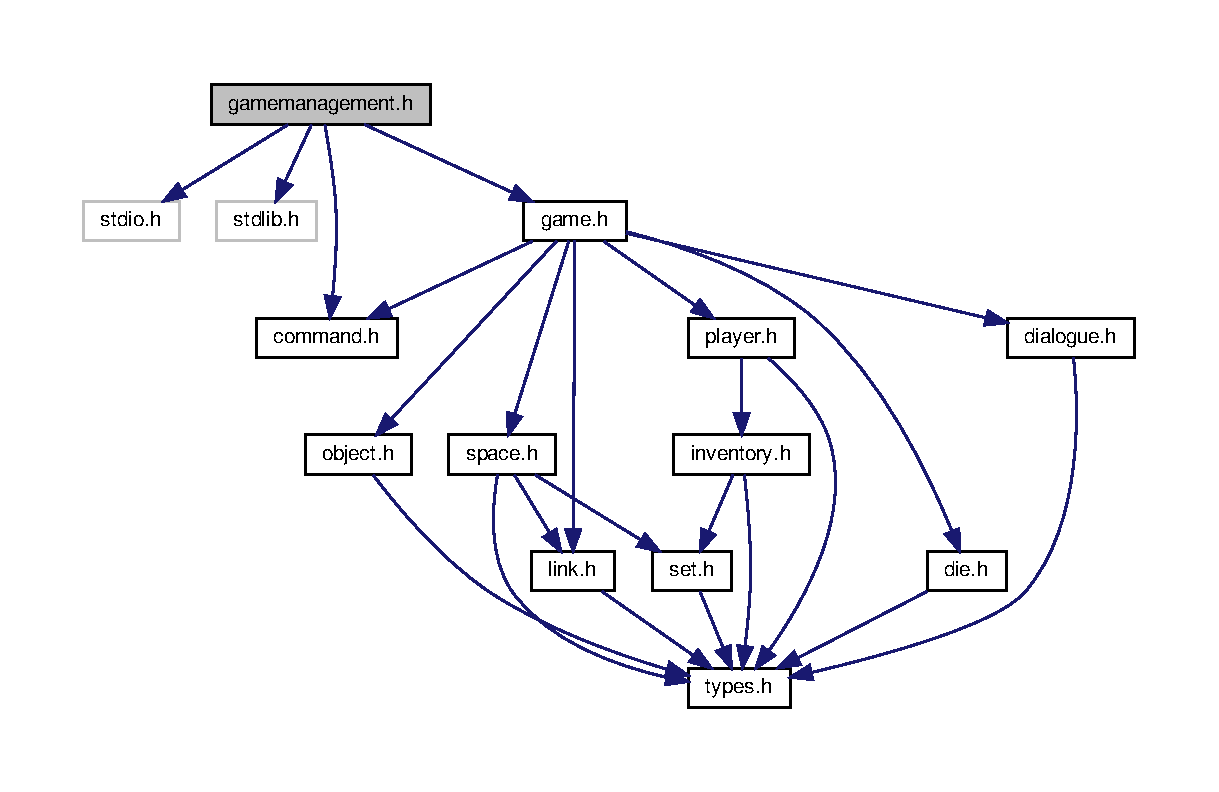
\includegraphics[width=350pt]{gamemanagement_8h__incl}
\end{center}
\end{figure}
This graph shows which files directly or indirectly include this file\+:
\nopagebreak
\begin{figure}[H]
\begin{center}
\leavevmode
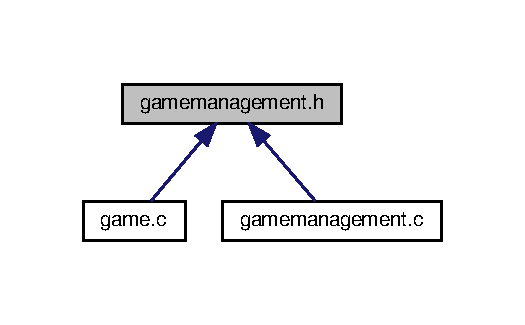
\includegraphics[width=252pt]{gamemanagement_8h__dep__incl}
\end{center}
\end{figure}
\subsection*{Functions}
\begin{DoxyCompactItemize}
\item 
\hyperlink{types_8h_a32c27cc471df37f4fc818d65de0a56c4}{S\+T\+A\+T\+US} \hyperlink{gamemanagement_8h_a0d01072a28b01545d36240cb8bd9d4f8}{game\+\_\+load\+\_\+spaces} (\hyperlink{game_8h_a57156d39c530aec3fba3a9dad8c2dc6a}{Game} $\ast$game, char $\ast$filename)
\begin{DoxyCompactList}\small\item\em it load the spaces to the game to be able to play \end{DoxyCompactList}\item 
\hyperlink{types_8h_a32c27cc471df37f4fc818d65de0a56c4}{S\+T\+A\+T\+US} \hyperlink{gamemanagement_8h_a66279ceefe2efe0967be248e8d0e0565}{game\+\_\+load\+\_\+objects} (\hyperlink{game_8h_a57156d39c530aec3fba3a9dad8c2dc6a}{Game} $\ast$game, char $\ast$filename)
\begin{DoxyCompactList}\small\item\em it load the objects to the game to be able to play \end{DoxyCompactList}\item 
\hyperlink{types_8h_a32c27cc471df37f4fc818d65de0a56c4}{S\+T\+A\+T\+US} \hyperlink{gamemanagement_8h_aab4103cf97109ac921f358858ca2684d}{game\+\_\+load\+\_\+links} (\hyperlink{game_8h_a57156d39c530aec3fba3a9dad8c2dc6a}{Game} $\ast$game, char $\ast$filename)
\begin{DoxyCompactList}\small\item\em it load the links to the game to be able to play \end{DoxyCompactList}\item 
\hyperlink{types_8h_a32c27cc471df37f4fc818d65de0a56c4}{S\+T\+A\+T\+US} \hyperlink{gamemanagement_8h_aa5c75aee9b0f84a7f3e194de25714df4}{gamemanagement\+\_\+save} (\hyperlink{game_8h_a57156d39c530aec3fba3a9dad8c2dc6a}{Game} $\ast$game, const char $\ast$dir)
\begin{DoxyCompactList}\small\item\em it saves the game \end{DoxyCompactList}\item 
\hyperlink{types_8h_a32c27cc471df37f4fc818d65de0a56c4}{S\+T\+A\+T\+US} \hyperlink{gamemanagement_8h_a6a7a09a84b7f206004e32985bba02af6}{gamemanagement\+\_\+load} (\hyperlink{game_8h_a57156d39c530aec3fba3a9dad8c2dc6a}{Game} $\ast$game, const char $\ast$dir)
\begin{DoxyCompactList}\small\item\em it loads the game \end{DoxyCompactList}\end{DoxyCompactItemize}


\subsection{Detailed Description}
It defines the header of gamemanagement. 

\begin{DoxyAuthor}{Author}
\end{DoxyAuthor}
\begin{DoxyVersion}{Version}
1.\+0 
\end{DoxyVersion}
\begin{DoxyDate}{Date}
09-\/02-\/2019 
\end{DoxyDate}
\begin{DoxyCopyright}{Copyright}
G\+NU Public License 
\end{DoxyCopyright}


\subsection{Function Documentation}
\mbox{\Hypertarget{gamemanagement_8h_aab4103cf97109ac921f358858ca2684d}\label{gamemanagement_8h_aab4103cf97109ac921f358858ca2684d}} 
\index{gamemanagement.\+h@{gamemanagement.\+h}!game\+\_\+load\+\_\+links@{game\+\_\+load\+\_\+links}}
\index{game\+\_\+load\+\_\+links@{game\+\_\+load\+\_\+links}!gamemanagement.\+h@{gamemanagement.\+h}}
\subsubsection{\texorpdfstring{game\+\_\+load\+\_\+links()}{game\_load\_links()}}
{\footnotesize\ttfamily \hyperlink{types_8h_a32c27cc471df37f4fc818d65de0a56c4}{S\+T\+A\+T\+US} game\+\_\+load\+\_\+links (\begin{DoxyParamCaption}\item[{\hyperlink{game_8h_a57156d39c530aec3fba3a9dad8c2dc6a}{Game} $\ast$}]{game,  }\item[{char $\ast$}]{filename }\end{DoxyParamCaption})}



it load the links to the game to be able to play 


\begin{DoxyParams}{Parameters}
{\em game} & \\
\hline
{\em filename} & \\
\hline
\end{DoxyParams}
\begin{DoxyReturn}{Returns}
OK, or E\+R\+R\+OR 
\end{DoxyReturn}
\mbox{\Hypertarget{gamemanagement_8h_a66279ceefe2efe0967be248e8d0e0565}\label{gamemanagement_8h_a66279ceefe2efe0967be248e8d0e0565}} 
\index{gamemanagement.\+h@{gamemanagement.\+h}!game\+\_\+load\+\_\+objects@{game\+\_\+load\+\_\+objects}}
\index{game\+\_\+load\+\_\+objects@{game\+\_\+load\+\_\+objects}!gamemanagement.\+h@{gamemanagement.\+h}}
\subsubsection{\texorpdfstring{game\+\_\+load\+\_\+objects()}{game\_load\_objects()}}
{\footnotesize\ttfamily \hyperlink{types_8h_a32c27cc471df37f4fc818d65de0a56c4}{S\+T\+A\+T\+US} game\+\_\+load\+\_\+objects (\begin{DoxyParamCaption}\item[{\hyperlink{game_8h_a57156d39c530aec3fba3a9dad8c2dc6a}{Game} $\ast$}]{game,  }\item[{char $\ast$}]{filename }\end{DoxyParamCaption})}



it load the objects to the game to be able to play 


\begin{DoxyParams}{Parameters}
{\em game} & \\
\hline
{\em filename} & \\
\hline
\end{DoxyParams}
\begin{DoxyReturn}{Returns}
OK, or E\+R\+R\+OR 
\end{DoxyReturn}
\mbox{\Hypertarget{gamemanagement_8h_a0d01072a28b01545d36240cb8bd9d4f8}\label{gamemanagement_8h_a0d01072a28b01545d36240cb8bd9d4f8}} 
\index{gamemanagement.\+h@{gamemanagement.\+h}!game\+\_\+load\+\_\+spaces@{game\+\_\+load\+\_\+spaces}}
\index{game\+\_\+load\+\_\+spaces@{game\+\_\+load\+\_\+spaces}!gamemanagement.\+h@{gamemanagement.\+h}}
\subsubsection{\texorpdfstring{game\+\_\+load\+\_\+spaces()}{game\_load\_spaces()}}
{\footnotesize\ttfamily \hyperlink{types_8h_a32c27cc471df37f4fc818d65de0a56c4}{S\+T\+A\+T\+US} game\+\_\+load\+\_\+spaces (\begin{DoxyParamCaption}\item[{\hyperlink{game_8h_a57156d39c530aec3fba3a9dad8c2dc6a}{Game} $\ast$}]{game,  }\item[{char $\ast$}]{filename }\end{DoxyParamCaption})}



it load the spaces to the game to be able to play 


\begin{DoxyParams}{Parameters}
{\em game} & \\
\hline
{\em filename} & \\
\hline
\end{DoxyParams}
\begin{DoxyReturn}{Returns}
OK, or E\+R\+R\+OR
\end{DoxyReturn}
it load the spaces to the game to be able to play

Private functions 
\begin{DoxyParams}{Parameters}
{\em game} & \\
\hline
{\em filename} & \\
\hline
\end{DoxyParams}
\begin{DoxyReturn}{Returns}
OK or E\+R\+R\+OR 
\end{DoxyReturn}
\mbox{\Hypertarget{gamemanagement_8h_a6a7a09a84b7f206004e32985bba02af6}\label{gamemanagement_8h_a6a7a09a84b7f206004e32985bba02af6}} 
\index{gamemanagement.\+h@{gamemanagement.\+h}!gamemanagement\+\_\+load@{gamemanagement\+\_\+load}}
\index{gamemanagement\+\_\+load@{gamemanagement\+\_\+load}!gamemanagement.\+h@{gamemanagement.\+h}}
\subsubsection{\texorpdfstring{gamemanagement\+\_\+load()}{gamemanagement\_load()}}
{\footnotesize\ttfamily \hyperlink{types_8h_a32c27cc471df37f4fc818d65de0a56c4}{S\+T\+A\+T\+US} gamemanagement\+\_\+load (\begin{DoxyParamCaption}\item[{\hyperlink{game_8h_a57156d39c530aec3fba3a9dad8c2dc6a}{Game} $\ast$}]{game,  }\item[{const char $\ast$}]{dir }\end{DoxyParamCaption})}



it loads the game 


\begin{DoxyParams}{Parameters}
{\em game} & \\
\hline
{\em dir} & \\
\hline
\end{DoxyParams}
\begin{DoxyReturn}{Returns}
OK, or E\+R\+R\+OR 
\end{DoxyReturn}
\mbox{\Hypertarget{gamemanagement_8h_aa5c75aee9b0f84a7f3e194de25714df4}\label{gamemanagement_8h_aa5c75aee9b0f84a7f3e194de25714df4}} 
\index{gamemanagement.\+h@{gamemanagement.\+h}!gamemanagement\+\_\+save@{gamemanagement\+\_\+save}}
\index{gamemanagement\+\_\+save@{gamemanagement\+\_\+save}!gamemanagement.\+h@{gamemanagement.\+h}}
\subsubsection{\texorpdfstring{gamemanagement\+\_\+save()}{gamemanagement\_save()}}
{\footnotesize\ttfamily \hyperlink{types_8h_a32c27cc471df37f4fc818d65de0a56c4}{S\+T\+A\+T\+US} gamemanagement\+\_\+save (\begin{DoxyParamCaption}\item[{\hyperlink{game_8h_a57156d39c530aec3fba3a9dad8c2dc6a}{Game} $\ast$}]{game,  }\item[{const char $\ast$}]{dir }\end{DoxyParamCaption})}



it saves the game 


\begin{DoxyParams}{Parameters}
{\em game} & \\
\hline
{\em dir} & \\
\hline
\end{DoxyParams}
\begin{DoxyReturn}{Returns}
OK, or E\+R\+R\+OR 
\end{DoxyReturn}


\hypertarget{graphic__engine_8c}{}\section{graphic\+\_\+engine.\+c File Reference}
\label{graphic__engine_8c}\index{graphic\+\_\+engine.\+c@{graphic\+\_\+engine.\+c}}


It defines the module of graphic\+\_\+engine.  


{\ttfamily \#include $<$stdlib.\+h$>$}\newline
{\ttfamily \#include $<$stdio.\+h$>$}\newline
{\ttfamily \#include \char`\"{}screen.\+h\char`\"{}}\newline
{\ttfamily \#include \char`\"{}graphic\+\_\+engine.\+h\char`\"{}}\newline
{\ttfamily \#include $<$string.\+h$>$}\newline
Include dependency graph for graphic\+\_\+engine.\+c\+:
\nopagebreak
\begin{figure}[H]
\begin{center}
\leavevmode
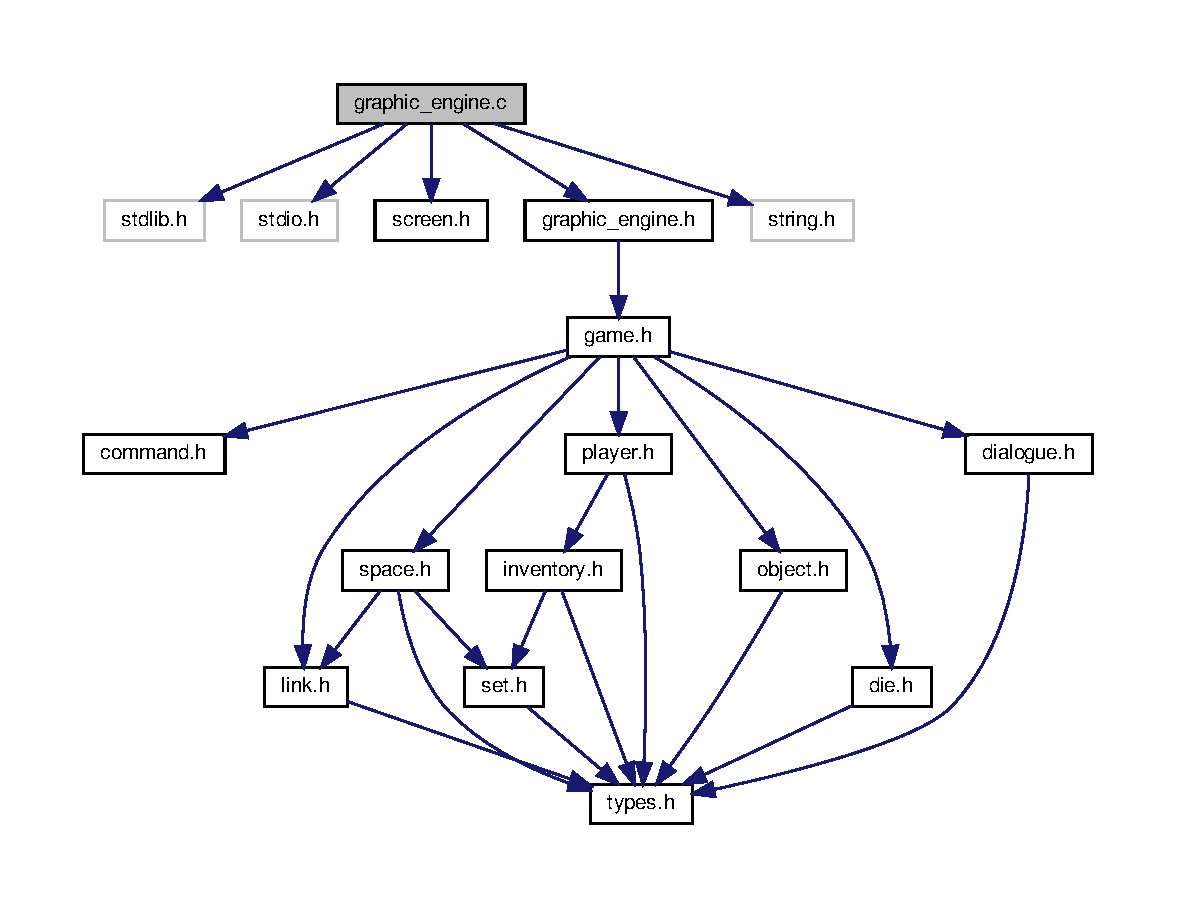
\includegraphics[width=350pt]{graphic__engine_8c__incl}
\end{center}
\end{figure}
\subsection*{Data Structures}
\begin{DoxyCompactItemize}
\item 
struct \hyperlink{struct__Graphic__engine}{\+\_\+\+Graphic\+\_\+engine}
\begin{DoxyCompactList}\small\item\em defines structure of graphic engine \end{DoxyCompactList}\end{DoxyCompactItemize}
\subsection*{Functions}
\begin{DoxyCompactItemize}
\item 
\hyperlink{graphic__engine_8h_ae1bc5cdbfce93098f066274fdea49af1}{Graphic\+\_\+engine} $\ast$ \hyperlink{graphic__engine_8c_a8c3d9abe7282bee1d77d23ea80a4bdec}{graphic\+\_\+engine\+\_\+create} ()
\begin{DoxyCompactList}\small\item\em it creates graphic engine in the game to be able to play \end{DoxyCompactList}\item 
void \hyperlink{graphic__engine_8c_a5a5eac4ef2033c5ad71aa6895f362f79}{graphic\+\_\+engine\+\_\+destroy} (\hyperlink{graphic__engine_8h_ae1bc5cdbfce93098f066274fdea49af1}{Graphic\+\_\+engine} $\ast$ge)
\begin{DoxyCompactList}\small\item\em destroys graphic engine in the game \end{DoxyCompactList}\item 
void \hyperlink{graphic__engine_8c_ab67b2c545a877fd98b29fafabbdb0509}{graphic\+\_\+engine\+\_\+paint\+\_\+game} (\hyperlink{graphic__engine_8h_ae1bc5cdbfce93098f066274fdea49af1}{Graphic\+\_\+engine} $\ast$ge, \hyperlink{game_8h_a57156d39c530aec3fba3a9dad8c2dc6a}{Game} $\ast$game, F\+I\+LE $\ast$f)
\begin{DoxyCompactList}\small\item\em paints graphic engine in the game \end{DoxyCompactList}\end{DoxyCompactItemize}


\subsection{Detailed Description}
It defines the module of graphic\+\_\+engine. 

\begin{DoxyAuthor}{Author}
\end{DoxyAuthor}
\begin{DoxyVersion}{Version}
3.\+0 
\end{DoxyVersion}
\begin{DoxyDate}{Date}
04-\/02-\/2019 
\end{DoxyDate}
\begin{DoxyCopyright}{Copyright}
G\+NU Public License 
\end{DoxyCopyright}


\subsection{Function Documentation}
\mbox{\Hypertarget{graphic__engine_8c_a8c3d9abe7282bee1d77d23ea80a4bdec}\label{graphic__engine_8c_a8c3d9abe7282bee1d77d23ea80a4bdec}} 
\index{graphic\+\_\+engine.\+c@{graphic\+\_\+engine.\+c}!graphic\+\_\+engine\+\_\+create@{graphic\+\_\+engine\+\_\+create}}
\index{graphic\+\_\+engine\+\_\+create@{graphic\+\_\+engine\+\_\+create}!graphic\+\_\+engine.\+c@{graphic\+\_\+engine.\+c}}
\subsubsection{\texorpdfstring{graphic\+\_\+engine\+\_\+create()}{graphic\_engine\_create()}}
{\footnotesize\ttfamily \hyperlink{graphic__engine_8h_ae1bc5cdbfce93098f066274fdea49af1}{Graphic\+\_\+engine}$\ast$ graphic\+\_\+engine\+\_\+create (\begin{DoxyParamCaption}{ }\end{DoxyParamCaption})}



it creates graphic engine in the game to be able to play 

\begin{DoxyReturn}{Returns}
graphic engine or in case of error N\+U\+LL 
\end{DoxyReturn}
\mbox{\Hypertarget{graphic__engine_8c_a5a5eac4ef2033c5ad71aa6895f362f79}\label{graphic__engine_8c_a5a5eac4ef2033c5ad71aa6895f362f79}} 
\index{graphic\+\_\+engine.\+c@{graphic\+\_\+engine.\+c}!graphic\+\_\+engine\+\_\+destroy@{graphic\+\_\+engine\+\_\+destroy}}
\index{graphic\+\_\+engine\+\_\+destroy@{graphic\+\_\+engine\+\_\+destroy}!graphic\+\_\+engine.\+c@{graphic\+\_\+engine.\+c}}
\subsubsection{\texorpdfstring{graphic\+\_\+engine\+\_\+destroy()}{graphic\_engine\_destroy()}}
{\footnotesize\ttfamily void graphic\+\_\+engine\+\_\+destroy (\begin{DoxyParamCaption}\item[{\hyperlink{graphic__engine_8h_ae1bc5cdbfce93098f066274fdea49af1}{Graphic\+\_\+engine} $\ast$}]{ge }\end{DoxyParamCaption})}



destroys graphic engine in the game 


\begin{DoxyParams}{Parameters}
{\em ge} & \\
\hline
\end{DoxyParams}
\begin{DoxyReturn}{Returns}
void 
\end{DoxyReturn}
\mbox{\Hypertarget{graphic__engine_8c_ab67b2c545a877fd98b29fafabbdb0509}\label{graphic__engine_8c_ab67b2c545a877fd98b29fafabbdb0509}} 
\index{graphic\+\_\+engine.\+c@{graphic\+\_\+engine.\+c}!graphic\+\_\+engine\+\_\+paint\+\_\+game@{graphic\+\_\+engine\+\_\+paint\+\_\+game}}
\index{graphic\+\_\+engine\+\_\+paint\+\_\+game@{graphic\+\_\+engine\+\_\+paint\+\_\+game}!graphic\+\_\+engine.\+c@{graphic\+\_\+engine.\+c}}
\subsubsection{\texorpdfstring{graphic\+\_\+engine\+\_\+paint\+\_\+game()}{graphic\_engine\_paint\_game()}}
{\footnotesize\ttfamily void graphic\+\_\+engine\+\_\+paint\+\_\+game (\begin{DoxyParamCaption}\item[{\hyperlink{graphic__engine_8h_ae1bc5cdbfce93098f066274fdea49af1}{Graphic\+\_\+engine} $\ast$}]{ge,  }\item[{\hyperlink{game_8h_a57156d39c530aec3fba3a9dad8c2dc6a}{Game} $\ast$}]{game,  }\item[{F\+I\+LE $\ast$}]{f }\end{DoxyParamCaption})}



paints graphic engine in the game 


\begin{DoxyParams}{Parameters}
{\em ge} & \\
\hline
{\em game} & \\
\hline
{\em f} & \\
\hline
\end{DoxyParams}
\begin{DoxyReturn}{Returns}
void 
\end{DoxyReturn}


\hypertarget{graphic__engine_8h}{}\section{graphic\+\_\+engine.\+h File Reference}
\label{graphic__engine_8h}\index{graphic\+\_\+engine.\+h@{graphic\+\_\+engine.\+h}}


It defines a textual graphic engine.  


{\ttfamily \#include \char`\"{}game.\+h\char`\"{}}\newline
Include dependency graph for graphic\+\_\+engine.\+h\+:
\nopagebreak
\begin{figure}[H]
\begin{center}
\leavevmode
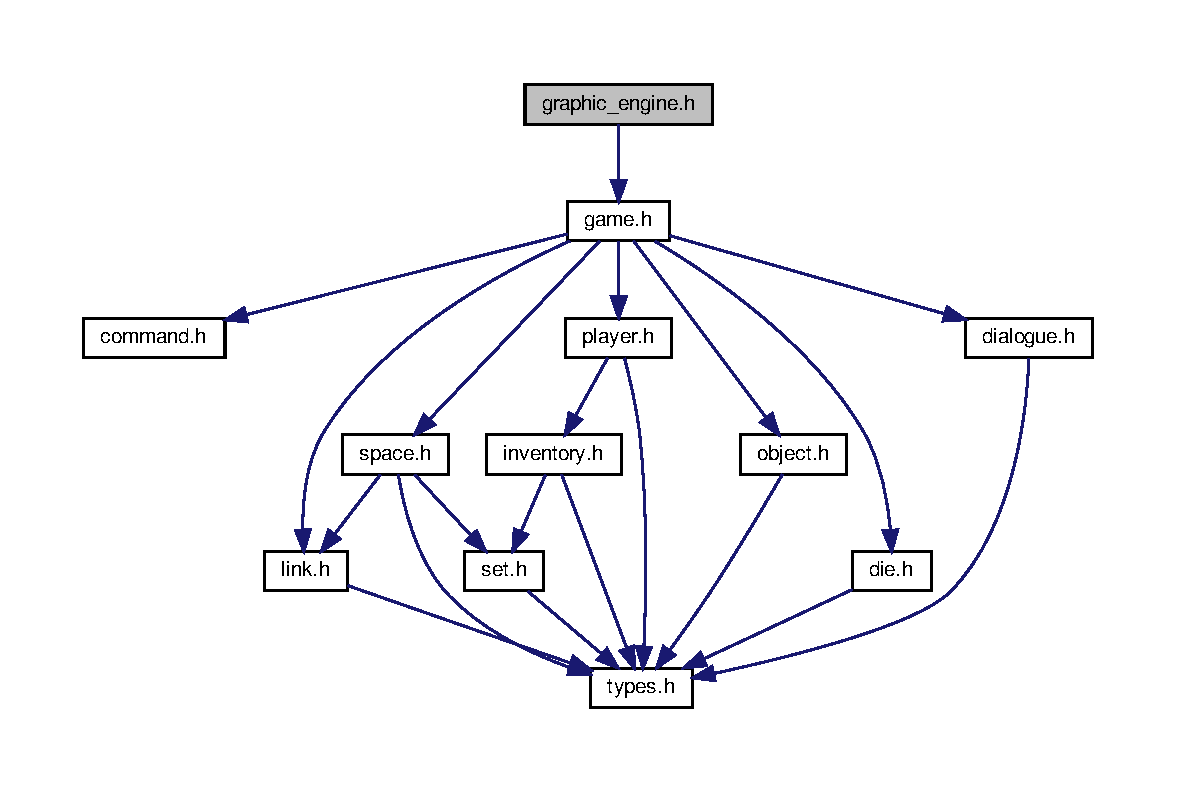
\includegraphics[width=350pt]{graphic__engine_8h__incl}
\end{center}
\end{figure}
This graph shows which files directly or indirectly include this file\+:
\nopagebreak
\begin{figure}[H]
\begin{center}
\leavevmode
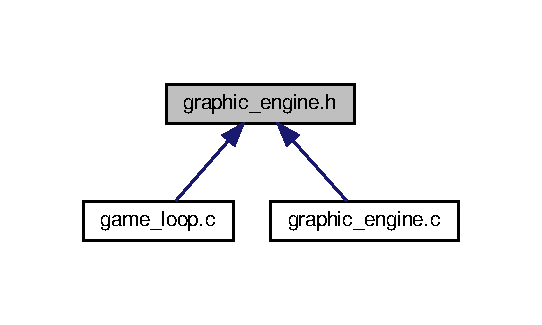
\includegraphics[width=260pt]{graphic__engine_8h__dep__incl}
\end{center}
\end{figure}
\subsection*{Typedefs}
\begin{DoxyCompactItemize}
\item 
\mbox{\Hypertarget{graphic__engine_8h_ae1bc5cdbfce93098f066274fdea49af1}\label{graphic__engine_8h_ae1bc5cdbfce93098f066274fdea49af1}} 
typedef struct \hyperlink{struct__Graphic__engine}{\+\_\+\+Graphic\+\_\+engine} \hyperlink{graphic__engine_8h_ae1bc5cdbfce93098f066274fdea49af1}{Graphic\+\_\+engine}
\begin{DoxyCompactList}\small\item\em defines the graphic engine structure \end{DoxyCompactList}\end{DoxyCompactItemize}
\subsection*{Functions}
\begin{DoxyCompactItemize}
\item 
\hyperlink{graphic__engine_8h_ae1bc5cdbfce93098f066274fdea49af1}{Graphic\+\_\+engine} $\ast$ \hyperlink{graphic__engine_8h_a8c3d9abe7282bee1d77d23ea80a4bdec}{graphic\+\_\+engine\+\_\+create} ()
\begin{DoxyCompactList}\small\item\em it creates graphic engine in the game to be able to play \end{DoxyCompactList}\item 
void \hyperlink{graphic__engine_8h_a5a5eac4ef2033c5ad71aa6895f362f79}{graphic\+\_\+engine\+\_\+destroy} (\hyperlink{graphic__engine_8h_ae1bc5cdbfce93098f066274fdea49af1}{Graphic\+\_\+engine} $\ast$ge)
\begin{DoxyCompactList}\small\item\em destroys graphic engine in the game \end{DoxyCompactList}\item 
void \hyperlink{graphic__engine_8h_ab67b2c545a877fd98b29fafabbdb0509}{graphic\+\_\+engine\+\_\+paint\+\_\+game} (\hyperlink{graphic__engine_8h_ae1bc5cdbfce93098f066274fdea49af1}{Graphic\+\_\+engine} $\ast$ge, \hyperlink{game_8h_a57156d39c530aec3fba3a9dad8c2dc6a}{Game} $\ast$game, F\+I\+LE $\ast$f)
\begin{DoxyCompactList}\small\item\em paints graphic engine in the game \end{DoxyCompactList}\item 
void \hyperlink{graphic__engine_8h_a112605879db4582a6d9cd6c12bd0e90c}{graphic\+\_\+engine\+\_\+write\+\_\+command} (\hyperlink{graphic__engine_8h_ae1bc5cdbfce93098f066274fdea49af1}{Graphic\+\_\+engine} $\ast$ge, char $\ast$str)
\begin{DoxyCompactList}\small\item\em write a command of graphic engine in the game \end{DoxyCompactList}\end{DoxyCompactItemize}


\subsection{Detailed Description}
It defines a textual graphic engine. 

\begin{DoxyAuthor}{Author}
\end{DoxyAuthor}
\begin{DoxyVersion}{Version}
2.\+0 
\end{DoxyVersion}
\begin{DoxyDate}{Date}
04-\/02-\/2019 
\end{DoxyDate}
\begin{DoxyCopyright}{Copyright}
G\+NU Public License 
\end{DoxyCopyright}


\subsection{Function Documentation}
\mbox{\Hypertarget{graphic__engine_8h_a8c3d9abe7282bee1d77d23ea80a4bdec}\label{graphic__engine_8h_a8c3d9abe7282bee1d77d23ea80a4bdec}} 
\index{graphic\+\_\+engine.\+h@{graphic\+\_\+engine.\+h}!graphic\+\_\+engine\+\_\+create@{graphic\+\_\+engine\+\_\+create}}
\index{graphic\+\_\+engine\+\_\+create@{graphic\+\_\+engine\+\_\+create}!graphic\+\_\+engine.\+h@{graphic\+\_\+engine.\+h}}
\subsubsection{\texorpdfstring{graphic\+\_\+engine\+\_\+create()}{graphic\_engine\_create()}}
{\footnotesize\ttfamily \hyperlink{graphic__engine_8h_ae1bc5cdbfce93098f066274fdea49af1}{Graphic\+\_\+engine}$\ast$ graphic\+\_\+engine\+\_\+create (\begin{DoxyParamCaption}{ }\end{DoxyParamCaption})}



it creates graphic engine in the game to be able to play 

\begin{DoxyReturn}{Returns}
graphic engine or in case of error N\+U\+LL 
\end{DoxyReturn}
\mbox{\Hypertarget{graphic__engine_8h_a5a5eac4ef2033c5ad71aa6895f362f79}\label{graphic__engine_8h_a5a5eac4ef2033c5ad71aa6895f362f79}} 
\index{graphic\+\_\+engine.\+h@{graphic\+\_\+engine.\+h}!graphic\+\_\+engine\+\_\+destroy@{graphic\+\_\+engine\+\_\+destroy}}
\index{graphic\+\_\+engine\+\_\+destroy@{graphic\+\_\+engine\+\_\+destroy}!graphic\+\_\+engine.\+h@{graphic\+\_\+engine.\+h}}
\subsubsection{\texorpdfstring{graphic\+\_\+engine\+\_\+destroy()}{graphic\_engine\_destroy()}}
{\footnotesize\ttfamily void graphic\+\_\+engine\+\_\+destroy (\begin{DoxyParamCaption}\item[{\hyperlink{graphic__engine_8h_ae1bc5cdbfce93098f066274fdea49af1}{Graphic\+\_\+engine} $\ast$}]{ge }\end{DoxyParamCaption})}



destroys graphic engine in the game 


\begin{DoxyParams}{Parameters}
{\em ge} & \\
\hline
\end{DoxyParams}
\begin{DoxyReturn}{Returns}
void 
\end{DoxyReturn}
\mbox{\Hypertarget{graphic__engine_8h_ab67b2c545a877fd98b29fafabbdb0509}\label{graphic__engine_8h_ab67b2c545a877fd98b29fafabbdb0509}} 
\index{graphic\+\_\+engine.\+h@{graphic\+\_\+engine.\+h}!graphic\+\_\+engine\+\_\+paint\+\_\+game@{graphic\+\_\+engine\+\_\+paint\+\_\+game}}
\index{graphic\+\_\+engine\+\_\+paint\+\_\+game@{graphic\+\_\+engine\+\_\+paint\+\_\+game}!graphic\+\_\+engine.\+h@{graphic\+\_\+engine.\+h}}
\subsubsection{\texorpdfstring{graphic\+\_\+engine\+\_\+paint\+\_\+game()}{graphic\_engine\_paint\_game()}}
{\footnotesize\ttfamily void graphic\+\_\+engine\+\_\+paint\+\_\+game (\begin{DoxyParamCaption}\item[{\hyperlink{graphic__engine_8h_ae1bc5cdbfce93098f066274fdea49af1}{Graphic\+\_\+engine} $\ast$}]{ge,  }\item[{\hyperlink{game_8h_a57156d39c530aec3fba3a9dad8c2dc6a}{Game} $\ast$}]{game,  }\item[{F\+I\+LE $\ast$}]{f }\end{DoxyParamCaption})}



paints graphic engine in the game 


\begin{DoxyParams}{Parameters}
{\em ge} & \\
\hline
{\em game} & \\
\hline
{\em f} & \\
\hline
\end{DoxyParams}
\begin{DoxyReturn}{Returns}
void 
\end{DoxyReturn}
\mbox{\Hypertarget{graphic__engine_8h_a112605879db4582a6d9cd6c12bd0e90c}\label{graphic__engine_8h_a112605879db4582a6d9cd6c12bd0e90c}} 
\index{graphic\+\_\+engine.\+h@{graphic\+\_\+engine.\+h}!graphic\+\_\+engine\+\_\+write\+\_\+command@{graphic\+\_\+engine\+\_\+write\+\_\+command}}
\index{graphic\+\_\+engine\+\_\+write\+\_\+command@{graphic\+\_\+engine\+\_\+write\+\_\+command}!graphic\+\_\+engine.\+h@{graphic\+\_\+engine.\+h}}
\subsubsection{\texorpdfstring{graphic\+\_\+engine\+\_\+write\+\_\+command()}{graphic\_engine\_write\_command()}}
{\footnotesize\ttfamily void graphic\+\_\+engine\+\_\+write\+\_\+command (\begin{DoxyParamCaption}\item[{\hyperlink{graphic__engine_8h_ae1bc5cdbfce93098f066274fdea49af1}{Graphic\+\_\+engine} $\ast$}]{ge,  }\item[{char $\ast$}]{str }\end{DoxyParamCaption})}



write a command of graphic engine in the game 


\begin{DoxyParams}{Parameters}
{\em ge} & \\
\hline
{\em str} & \\
\hline
\end{DoxyParams}
\begin{DoxyReturn}{Returns}
void 
\end{DoxyReturn}


\hypertarget{inventory_8c}{}\section{inventory.\+c File Reference}
\label{inventory_8c}\index{inventory.\+c@{inventory.\+c}}


It implements the inventory module,it keeps the drop objects.  


{\ttfamily \#include $<$stdio.\+h$>$}\newline
{\ttfamily \#include $<$stdlib.\+h$>$}\newline
{\ttfamily \#include \char`\"{}set.\+h\char`\"{}}\newline
{\ttfamily \#include \char`\"{}types.\+h\char`\"{}}\newline
{\ttfamily \#include \char`\"{}inventory.\+h\char`\"{}}\newline
Include dependency graph for inventory.\+c\+:
\nopagebreak
\begin{figure}[H]
\begin{center}
\leavevmode
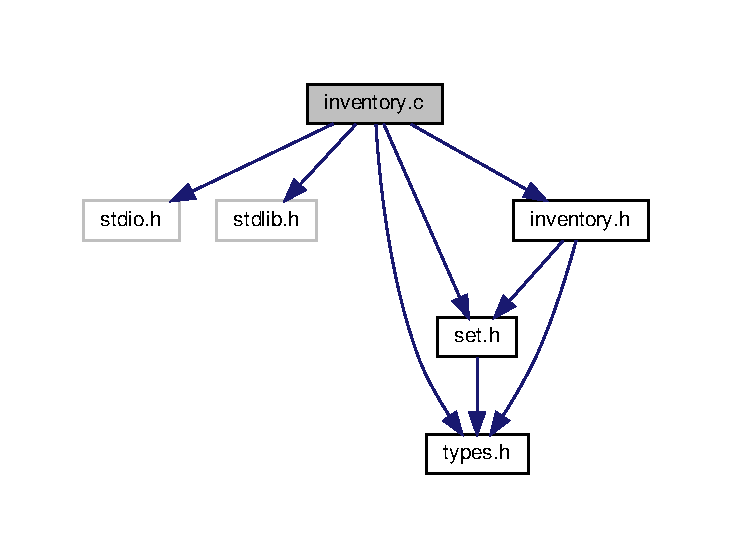
\includegraphics[width=350pt]{inventory_8c__incl}
\end{center}
\end{figure}
\subsection*{Data Structures}
\begin{DoxyCompactItemize}
\item 
struct \hyperlink{struct__Bag}{\+\_\+\+Bag}
\begin{DoxyCompactList}\small\item\em defines structure of bag \end{DoxyCompactList}\end{DoxyCompactItemize}
\subsection*{Functions}
\begin{DoxyCompactItemize}
\item 
\hyperlink{inventory_8h_a96eaad8b37d9b6e19ddc373ec38c751e}{Bag} $\ast$ \hyperlink{inventory_8c_a7a7a920b704bd2432f665ac0268be447}{bag\+\_\+create} ()
\begin{DoxyCompactList}\small\item\em create a bag \end{DoxyCompactList}\item 
void \hyperlink{inventory_8c_aada9a87f8de0d01f6b896dcc2e2bac43}{bag\+\_\+destroy} (\hyperlink{inventory_8h_a96eaad8b37d9b6e19ddc373ec38c751e}{Bag} $\ast$bag)
\begin{DoxyCompactList}\small\item\em destroy bag \end{DoxyCompactList}\item 
\hyperlink{types_8h_a32c27cc471df37f4fc818d65de0a56c4}{S\+T\+A\+T\+US} \hyperlink{inventory_8c_adb716c6c8c93013fee634bad8ad8837f}{bag\+\_\+add\+Obj} (\hyperlink{inventory_8h_a96eaad8b37d9b6e19ddc373ec38c751e}{Bag} $\ast$bag, \hyperlink{types_8h_a845e604fb28f7e3d97549da3448149d3}{Id} obj)
\begin{DoxyCompactList}\small\item\em add an object \end{DoxyCompactList}\item 
\hyperlink{types_8h_a32c27cc471df37f4fc818d65de0a56c4}{S\+T\+A\+T\+US} \hyperlink{inventory_8c_aaa55527dd33257b50abe049ca1c4cab7}{bag\+\_\+remove\+Obj} (\hyperlink{inventory_8h_a96eaad8b37d9b6e19ddc373ec38c751e}{Bag} $\ast$bag, \hyperlink{types_8h_a845e604fb28f7e3d97549da3448149d3}{Id} id)
\begin{DoxyCompactList}\small\item\em remove an object \end{DoxyCompactList}\item 
\hyperlink{types_8h_a3e5b8192e7d9ffaf3542f1210aec18dd}{B\+O\+OL} \hyperlink{inventory_8c_a025c9a4d21c3e5ad3d1beb3ffcb0c61a}{bag\+\_\+check\+Obj} (\hyperlink{inventory_8h_a96eaad8b37d9b6e19ddc373ec38c751e}{Bag} $\ast$bag, int pos)
\begin{DoxyCompactList}\small\item\em checks objects \end{DoxyCompactList}\item 
int \hyperlink{inventory_8c_aa9cd4c1707e337436c5c47de3243f4bd}{bag\+\_\+num\+Obj} (\hyperlink{inventory_8h_a96eaad8b37d9b6e19ddc373ec38c751e}{Bag} $\ast$bag)
\begin{DoxyCompactList}\small\item\em G\+ET T\+HE N\+U\+M\+B\+ER OF A\+L\+L\+O\+C\+A\+T\+ED O\+B\+J\+E\+CT. \end{DoxyCompactList}\item 
\hyperlink{types_8h_a32c27cc471df37f4fc818d65de0a56c4}{S\+T\+A\+T\+US} \hyperlink{inventory_8c_a0bdd587bf81c5aaabbd1b2e474f078fb}{bag\+\_\+set\+Max\+Obj} (\hyperlink{inventory_8h_a96eaad8b37d9b6e19ddc373ec38c751e}{Bag} $\ast$bag, int max\+\_\+obj)
\begin{DoxyCompactList}\small\item\em set max objects in game \end{DoxyCompactList}\item 
\hyperlink{types_8h_a845e604fb28f7e3d97549da3448149d3}{Id} \hyperlink{inventory_8c_a7c53a93839697e3f40a5e5105b195bf2}{bag\+\_\+get\+Object} (\hyperlink{inventory_8h_a96eaad8b37d9b6e19ddc373ec38c751e}{Bag} $\ast$bag, int position)
\begin{DoxyCompactList}\small\item\em get objcet bag in game \end{DoxyCompactList}\item 
\hyperlink{types_8h_a32c27cc471df37f4fc818d65de0a56c4}{S\+T\+A\+T\+US} \hyperlink{inventory_8c_a996300fd5ac9e16d1f72cf7c6895fa2b}{bag\+\_\+set\+Object} (\hyperlink{inventory_8h_a96eaad8b37d9b6e19ddc373ec38c751e}{Bag} $\ast$bag, \hyperlink{types_8h_a845e604fb28f7e3d97549da3448149d3}{Id} id, int position)
\begin{DoxyCompactList}\small\item\em set id psoition of bag in game \end{DoxyCompactList}\item 
int \hyperlink{inventory_8c_a776ffdc273b024c5d02355d4ee1d13e3}{bag\+\_\+get\+Max\+Obj} (\hyperlink{inventory_8h_a96eaad8b37d9b6e19ddc373ec38c751e}{Bag} $\ast$bag)
\begin{DoxyCompactList}\small\item\em G\+ET M\+AX O\+B\+J\+E\+CT. \end{DoxyCompactList}\item 
void \hyperlink{inventory_8c_a640f8257f45259075f0fe5fbdfca2dd6}{bag\+\_\+print} (\hyperlink{inventory_8h_a96eaad8b37d9b6e19ddc373ec38c751e}{Bag} $\ast$bag)
\begin{DoxyCompactList}\small\item\em prints the bag in the game \end{DoxyCompactList}\end{DoxyCompactItemize}


\subsection{Detailed Description}
It implements the inventory module,it keeps the drop objects. 

\begin{DoxyAuthor}{Author}
\end{DoxyAuthor}
\begin{DoxyVersion}{Version}
1.\+0 
\end{DoxyVersion}
\begin{DoxyDate}{Date}
28-\/03-\/2019 
\end{DoxyDate}
\begin{DoxyCopyright}{Copyright}
G\+NU Public License 
\end{DoxyCopyright}


\subsection{Function Documentation}
\mbox{\Hypertarget{inventory_8c_adb716c6c8c93013fee634bad8ad8837f}\label{inventory_8c_adb716c6c8c93013fee634bad8ad8837f}} 
\index{inventory.\+c@{inventory.\+c}!bag\+\_\+add\+Obj@{bag\+\_\+add\+Obj}}
\index{bag\+\_\+add\+Obj@{bag\+\_\+add\+Obj}!inventory.\+c@{inventory.\+c}}
\subsubsection{\texorpdfstring{bag\+\_\+add\+Obj()}{bag\_addObj()}}
{\footnotesize\ttfamily \hyperlink{types_8h_a32c27cc471df37f4fc818d65de0a56c4}{S\+T\+A\+T\+US} bag\+\_\+add\+Obj (\begin{DoxyParamCaption}\item[{\hyperlink{inventory_8h_a96eaad8b37d9b6e19ddc373ec38c751e}{Bag} $\ast$}]{bag,  }\item[{\hyperlink{types_8h_a845e604fb28f7e3d97549da3448149d3}{Id}}]{obj }\end{DoxyParamCaption})}



add an object 


\begin{DoxyParams}{Parameters}
{\em bag} & \\
\hline
{\em obj} & \\
\hline
\end{DoxyParams}
\begin{DoxyReturn}{Returns}
OK, or E\+R\+R\+OR 
\end{DoxyReturn}
\mbox{\Hypertarget{inventory_8c_a025c9a4d21c3e5ad3d1beb3ffcb0c61a}\label{inventory_8c_a025c9a4d21c3e5ad3d1beb3ffcb0c61a}} 
\index{inventory.\+c@{inventory.\+c}!bag\+\_\+check\+Obj@{bag\+\_\+check\+Obj}}
\index{bag\+\_\+check\+Obj@{bag\+\_\+check\+Obj}!inventory.\+c@{inventory.\+c}}
\subsubsection{\texorpdfstring{bag\+\_\+check\+Obj()}{bag\_checkObj()}}
{\footnotesize\ttfamily \hyperlink{types_8h_a3e5b8192e7d9ffaf3542f1210aec18dd}{B\+O\+OL} bag\+\_\+check\+Obj (\begin{DoxyParamCaption}\item[{\hyperlink{inventory_8h_a96eaad8b37d9b6e19ddc373ec38c751e}{Bag} $\ast$}]{bag,  }\item[{int}]{pos }\end{DoxyParamCaption})}



checks objects 


\begin{DoxyParams}{Parameters}
{\em bag} & \\
\hline
{\em pos} & \\
\hline
\end{DoxyParams}
\begin{DoxyReturn}{Returns}
T\+R\+UE or F\+A\+L\+SE 
\end{DoxyReturn}
\mbox{\Hypertarget{inventory_8c_a7a7a920b704bd2432f665ac0268be447}\label{inventory_8c_a7a7a920b704bd2432f665ac0268be447}} 
\index{inventory.\+c@{inventory.\+c}!bag\+\_\+create@{bag\+\_\+create}}
\index{bag\+\_\+create@{bag\+\_\+create}!inventory.\+c@{inventory.\+c}}
\subsubsection{\texorpdfstring{bag\+\_\+create()}{bag\_create()}}
{\footnotesize\ttfamily \hyperlink{inventory_8h_a96eaad8b37d9b6e19ddc373ec38c751e}{Bag}$\ast$ bag\+\_\+create (\begin{DoxyParamCaption}{ }\end{DoxyParamCaption})}



create a bag 

\begin{DoxyReturn}{Returns}
bag, in case of error N\+U\+LL 
\end{DoxyReturn}
\mbox{\Hypertarget{inventory_8c_aada9a87f8de0d01f6b896dcc2e2bac43}\label{inventory_8c_aada9a87f8de0d01f6b896dcc2e2bac43}} 
\index{inventory.\+c@{inventory.\+c}!bag\+\_\+destroy@{bag\+\_\+destroy}}
\index{bag\+\_\+destroy@{bag\+\_\+destroy}!inventory.\+c@{inventory.\+c}}
\subsubsection{\texorpdfstring{bag\+\_\+destroy()}{bag\_destroy()}}
{\footnotesize\ttfamily void bag\+\_\+destroy (\begin{DoxyParamCaption}\item[{\hyperlink{inventory_8h_a96eaad8b37d9b6e19ddc373ec38c751e}{Bag} $\ast$}]{bag }\end{DoxyParamCaption})}



destroy bag 


\begin{DoxyParams}{Parameters}
{\em bag} & \\
\hline
\end{DoxyParams}
\begin{DoxyReturn}{Returns}
bag, in case of error N\+U\+LL 
\end{DoxyReturn}
\mbox{\Hypertarget{inventory_8c_a776ffdc273b024c5d02355d4ee1d13e3}\label{inventory_8c_a776ffdc273b024c5d02355d4ee1d13e3}} 
\index{inventory.\+c@{inventory.\+c}!bag\+\_\+get\+Max\+Obj@{bag\+\_\+get\+Max\+Obj}}
\index{bag\+\_\+get\+Max\+Obj@{bag\+\_\+get\+Max\+Obj}!inventory.\+c@{inventory.\+c}}
\subsubsection{\texorpdfstring{bag\+\_\+get\+Max\+Obj()}{bag\_getMaxObj()}}
{\footnotesize\ttfamily int bag\+\_\+get\+Max\+Obj (\begin{DoxyParamCaption}\item[{\hyperlink{inventory_8h_a96eaad8b37d9b6e19ddc373ec38c751e}{Bag} $\ast$}]{bag }\end{DoxyParamCaption})}



G\+ET M\+AX O\+B\+J\+E\+CT. 


\begin{DoxyParams}{Parameters}
{\em bag} & \\
\hline
\end{DoxyParams}
\begin{DoxyReturn}{Returns}
N\+U\+M\+B\+ER OF M\+AX O\+B\+J\+E\+CT or -\/1 in case of error 
\end{DoxyReturn}
\mbox{\Hypertarget{inventory_8c_a7c53a93839697e3f40a5e5105b195bf2}\label{inventory_8c_a7c53a93839697e3f40a5e5105b195bf2}} 
\index{inventory.\+c@{inventory.\+c}!bag\+\_\+get\+Object@{bag\+\_\+get\+Object}}
\index{bag\+\_\+get\+Object@{bag\+\_\+get\+Object}!inventory.\+c@{inventory.\+c}}
\subsubsection{\texorpdfstring{bag\+\_\+get\+Object()}{bag\_getObject()}}
{\footnotesize\ttfamily \hyperlink{types_8h_a845e604fb28f7e3d97549da3448149d3}{Id} bag\+\_\+get\+Object (\begin{DoxyParamCaption}\item[{\hyperlink{inventory_8h_a96eaad8b37d9b6e19ddc373ec38c751e}{Bag} $\ast$}]{bag,  }\item[{int}]{position }\end{DoxyParamCaption})}



get objcet bag in game 


\begin{DoxyParams}{Parameters}
{\em bag} & \\
\hline
{\em position} & \\
\hline
\end{DoxyParams}
\begin{DoxyReturn}{Returns}
bah or in case of error N\+U\+LL 
\end{DoxyReturn}
\mbox{\Hypertarget{inventory_8c_aa9cd4c1707e337436c5c47de3243f4bd}\label{inventory_8c_aa9cd4c1707e337436c5c47de3243f4bd}} 
\index{inventory.\+c@{inventory.\+c}!bag\+\_\+num\+Obj@{bag\+\_\+num\+Obj}}
\index{bag\+\_\+num\+Obj@{bag\+\_\+num\+Obj}!inventory.\+c@{inventory.\+c}}
\subsubsection{\texorpdfstring{bag\+\_\+num\+Obj()}{bag\_numObj()}}
{\footnotesize\ttfamily int bag\+\_\+num\+Obj (\begin{DoxyParamCaption}\item[{\hyperlink{inventory_8h_a96eaad8b37d9b6e19ddc373ec38c751e}{Bag} $\ast$}]{bag }\end{DoxyParamCaption})}



G\+ET T\+HE N\+U\+M\+B\+ER OF A\+L\+L\+O\+C\+A\+T\+ED O\+B\+J\+E\+CT. 


\begin{DoxyParams}{Parameters}
{\em bag} & \\
\hline
\end{DoxyParams}
\begin{DoxyReturn}{Returns}
N\+U\+M\+B\+ER OF A\+L\+L\+O\+C\+A\+T\+ED O\+B\+J\+E\+CT or -\/1 in case of error 
\end{DoxyReturn}
\mbox{\Hypertarget{inventory_8c_a640f8257f45259075f0fe5fbdfca2dd6}\label{inventory_8c_a640f8257f45259075f0fe5fbdfca2dd6}} 
\index{inventory.\+c@{inventory.\+c}!bag\+\_\+print@{bag\+\_\+print}}
\index{bag\+\_\+print@{bag\+\_\+print}!inventory.\+c@{inventory.\+c}}
\subsubsection{\texorpdfstring{bag\+\_\+print()}{bag\_print()}}
{\footnotesize\ttfamily void bag\+\_\+print (\begin{DoxyParamCaption}\item[{\hyperlink{inventory_8h_a96eaad8b37d9b6e19ddc373ec38c751e}{Bag} $\ast$}]{bag }\end{DoxyParamCaption})}



prints the bag in the game 


\begin{DoxyParams}{Parameters}
{\em bag} & \\
\hline
\end{DoxyParams}
\begin{DoxyReturn}{Returns}
void 
\end{DoxyReturn}
\mbox{\Hypertarget{inventory_8c_aaa55527dd33257b50abe049ca1c4cab7}\label{inventory_8c_aaa55527dd33257b50abe049ca1c4cab7}} 
\index{inventory.\+c@{inventory.\+c}!bag\+\_\+remove\+Obj@{bag\+\_\+remove\+Obj}}
\index{bag\+\_\+remove\+Obj@{bag\+\_\+remove\+Obj}!inventory.\+c@{inventory.\+c}}
\subsubsection{\texorpdfstring{bag\+\_\+remove\+Obj()}{bag\_removeObj()}}
{\footnotesize\ttfamily \hyperlink{types_8h_a32c27cc471df37f4fc818d65de0a56c4}{S\+T\+A\+T\+US} bag\+\_\+remove\+Obj (\begin{DoxyParamCaption}\item[{\hyperlink{inventory_8h_a96eaad8b37d9b6e19ddc373ec38c751e}{Bag} $\ast$}]{bag,  }\item[{\hyperlink{types_8h_a845e604fb28f7e3d97549da3448149d3}{Id}}]{id }\end{DoxyParamCaption})}



remove an object 


\begin{DoxyParams}{Parameters}
{\em bag} & \\
\hline
{\em id} & \\
\hline
\end{DoxyParams}
\begin{DoxyReturn}{Returns}
OK, or E\+R\+R\+OR 
\end{DoxyReturn}
\mbox{\Hypertarget{inventory_8c_a0bdd587bf81c5aaabbd1b2e474f078fb}\label{inventory_8c_a0bdd587bf81c5aaabbd1b2e474f078fb}} 
\index{inventory.\+c@{inventory.\+c}!bag\+\_\+set\+Max\+Obj@{bag\+\_\+set\+Max\+Obj}}
\index{bag\+\_\+set\+Max\+Obj@{bag\+\_\+set\+Max\+Obj}!inventory.\+c@{inventory.\+c}}
\subsubsection{\texorpdfstring{bag\+\_\+set\+Max\+Obj()}{bag\_setMaxObj()}}
{\footnotesize\ttfamily \hyperlink{types_8h_a32c27cc471df37f4fc818d65de0a56c4}{S\+T\+A\+T\+US} bag\+\_\+set\+Max\+Obj (\begin{DoxyParamCaption}\item[{\hyperlink{inventory_8h_a96eaad8b37d9b6e19ddc373ec38c751e}{Bag} $\ast$}]{bag,  }\item[{int}]{max\+\_\+obj }\end{DoxyParamCaption})}



set max objects in game 


\begin{DoxyParams}{Parameters}
{\em bag} & \\
\hline
{\em max\+\_\+obj} & \\
\hline
\end{DoxyParams}
\begin{DoxyReturn}{Returns}
OK, or E\+R\+R\+OR 
\end{DoxyReturn}
\mbox{\Hypertarget{inventory_8c_a996300fd5ac9e16d1f72cf7c6895fa2b}\label{inventory_8c_a996300fd5ac9e16d1f72cf7c6895fa2b}} 
\index{inventory.\+c@{inventory.\+c}!bag\+\_\+set\+Object@{bag\+\_\+set\+Object}}
\index{bag\+\_\+set\+Object@{bag\+\_\+set\+Object}!inventory.\+c@{inventory.\+c}}
\subsubsection{\texorpdfstring{bag\+\_\+set\+Object()}{bag\_setObject()}}
{\footnotesize\ttfamily \hyperlink{types_8h_a32c27cc471df37f4fc818d65de0a56c4}{S\+T\+A\+T\+US} bag\+\_\+set\+Object (\begin{DoxyParamCaption}\item[{\hyperlink{inventory_8h_a96eaad8b37d9b6e19ddc373ec38c751e}{Bag} $\ast$}]{bag,  }\item[{\hyperlink{types_8h_a845e604fb28f7e3d97549da3448149d3}{Id}}]{id,  }\item[{int}]{position }\end{DoxyParamCaption})}



set id psoition of bag in game 


\begin{DoxyParams}{Parameters}
{\em bag} & \\
\hline
{\em id} & \\
\hline
{\em position} & \\
\hline
\end{DoxyParams}
\begin{DoxyReturn}{Returns}
OK, or E\+R\+R\+OR 
\end{DoxyReturn}


\hypertarget{inventory_8h}{}\section{inventory.\+h File Reference}
\label{inventory_8h}\index{inventory.\+h@{inventory.\+h}}


It defines the header of inventory.  


{\ttfamily \#include \char`\"{}types.\+h\char`\"{}}\newline
{\ttfamily \#include \char`\"{}set.\+h\char`\"{}}\newline
Include dependency graph for inventory.\+h\+:
\nopagebreak
\begin{figure}[H]
\begin{center}
\leavevmode
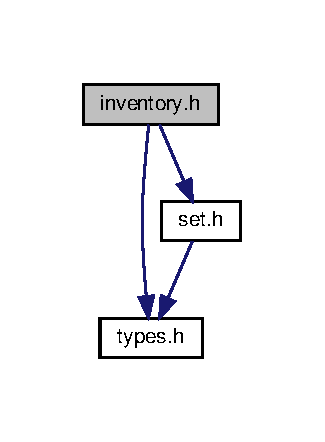
\includegraphics[width=156pt]{inventory_8h__incl}
\end{center}
\end{figure}
This graph shows which files directly or indirectly include this file\+:
\nopagebreak
\begin{figure}[H]
\begin{center}
\leavevmode
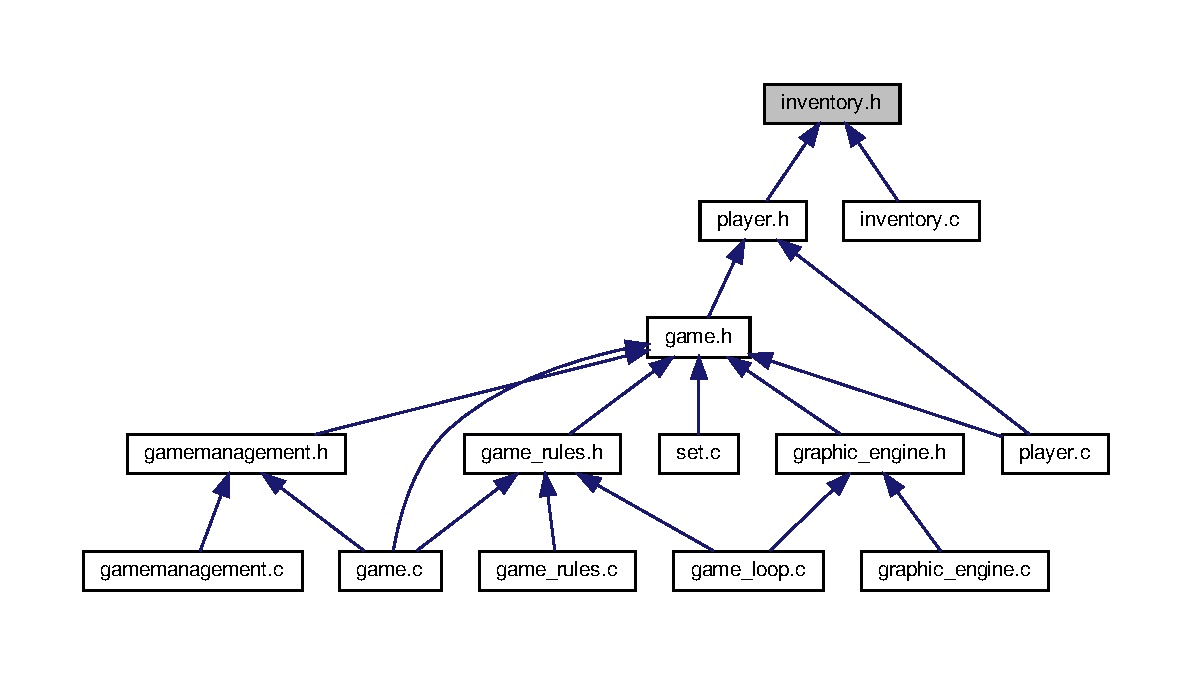
\includegraphics[width=214pt]{inventory_8h__dep__incl}
\end{center}
\end{figure}
\subsection*{Typedefs}
\begin{DoxyCompactItemize}
\item 
\mbox{\Hypertarget{inventory_8h_a96eaad8b37d9b6e19ddc373ec38c751e}\label{inventory_8h_a96eaad8b37d9b6e19ddc373ec38c751e}} 
typedef struct \hyperlink{struct__Bag}{\+\_\+\+Bag} \hyperlink{inventory_8h_a96eaad8b37d9b6e19ddc373ec38c751e}{Bag}
\begin{DoxyCompactList}\small\item\em defines the bag structure \end{DoxyCompactList}\end{DoxyCompactItemize}
\subsection*{Functions}
\begin{DoxyCompactItemize}
\item 
\hyperlink{inventory_8h_a96eaad8b37d9b6e19ddc373ec38c751e}{Bag} $\ast$ \hyperlink{inventory_8h_a7a7a920b704bd2432f665ac0268be447}{bag\+\_\+create} ()
\begin{DoxyCompactList}\small\item\em create a bag \end{DoxyCompactList}\item 
void \hyperlink{inventory_8h_aada9a87f8de0d01f6b896dcc2e2bac43}{bag\+\_\+destroy} (\hyperlink{inventory_8h_a96eaad8b37d9b6e19ddc373ec38c751e}{Bag} $\ast$bag)
\begin{DoxyCompactList}\small\item\em destroy bag \end{DoxyCompactList}\item 
\hyperlink{types_8h_a32c27cc471df37f4fc818d65de0a56c4}{S\+T\+A\+T\+US} \hyperlink{inventory_8h_adb716c6c8c93013fee634bad8ad8837f}{bag\+\_\+add\+Obj} (\hyperlink{inventory_8h_a96eaad8b37d9b6e19ddc373ec38c751e}{Bag} $\ast$bag, \hyperlink{types_8h_a845e604fb28f7e3d97549da3448149d3}{Id} obj)
\begin{DoxyCompactList}\small\item\em add an object \end{DoxyCompactList}\item 
\hyperlink{types_8h_a32c27cc471df37f4fc818d65de0a56c4}{S\+T\+A\+T\+US} \hyperlink{inventory_8h_aaa55527dd33257b50abe049ca1c4cab7}{bag\+\_\+remove\+Obj} (\hyperlink{inventory_8h_a96eaad8b37d9b6e19ddc373ec38c751e}{Bag} $\ast$bag, \hyperlink{types_8h_a845e604fb28f7e3d97549da3448149d3}{Id} id)
\begin{DoxyCompactList}\small\item\em remove an object \end{DoxyCompactList}\item 
\hyperlink{types_8h_a3e5b8192e7d9ffaf3542f1210aec18dd}{B\+O\+OL} \hyperlink{inventory_8h_a025c9a4d21c3e5ad3d1beb3ffcb0c61a}{bag\+\_\+check\+Obj} (\hyperlink{inventory_8h_a96eaad8b37d9b6e19ddc373ec38c751e}{Bag} $\ast$bag, int pos)
\begin{DoxyCompactList}\small\item\em checks objects \end{DoxyCompactList}\item 
int \hyperlink{inventory_8h_aa9cd4c1707e337436c5c47de3243f4bd}{bag\+\_\+num\+Obj} (\hyperlink{inventory_8h_a96eaad8b37d9b6e19ddc373ec38c751e}{Bag} $\ast$bag)
\begin{DoxyCompactList}\small\item\em G\+ET T\+HE N\+U\+M\+B\+ER OF A\+L\+L\+O\+C\+A\+T\+ED O\+B\+J\+E\+CT. \end{DoxyCompactList}\item 
\hyperlink{types_8h_a32c27cc471df37f4fc818d65de0a56c4}{S\+T\+A\+T\+US} \hyperlink{inventory_8h_a0bdd587bf81c5aaabbd1b2e474f078fb}{bag\+\_\+set\+Max\+Obj} (\hyperlink{inventory_8h_a96eaad8b37d9b6e19ddc373ec38c751e}{Bag} $\ast$bag, int max\+\_\+obj)
\begin{DoxyCompactList}\small\item\em set max objects in game \end{DoxyCompactList}\item 
int \hyperlink{inventory_8h_a776ffdc273b024c5d02355d4ee1d13e3}{bag\+\_\+get\+Max\+Obj} (\hyperlink{inventory_8h_a96eaad8b37d9b6e19ddc373ec38c751e}{Bag} $\ast$bag)
\begin{DoxyCompactList}\small\item\em G\+ET M\+AX O\+B\+J\+E\+CT. \end{DoxyCompactList}\item 
\hyperlink{types_8h_a845e604fb28f7e3d97549da3448149d3}{Id} \hyperlink{inventory_8h_a7c53a93839697e3f40a5e5105b195bf2}{bag\+\_\+get\+Object} (\hyperlink{inventory_8h_a96eaad8b37d9b6e19ddc373ec38c751e}{Bag} $\ast$bag, int position)
\begin{DoxyCompactList}\small\item\em get objcet bag in game \end{DoxyCompactList}\item 
\hyperlink{types_8h_a32c27cc471df37f4fc818d65de0a56c4}{S\+T\+A\+T\+US} \hyperlink{inventory_8h_a996300fd5ac9e16d1f72cf7c6895fa2b}{bag\+\_\+set\+Object} (\hyperlink{inventory_8h_a96eaad8b37d9b6e19ddc373ec38c751e}{Bag} $\ast$bag, \hyperlink{types_8h_a845e604fb28f7e3d97549da3448149d3}{Id} id, int position)
\begin{DoxyCompactList}\small\item\em set id psoition of bag in game \end{DoxyCompactList}\item 
void \hyperlink{inventory_8h_a640f8257f45259075f0fe5fbdfca2dd6}{bag\+\_\+print} (\hyperlink{inventory_8h_a96eaad8b37d9b6e19ddc373ec38c751e}{Bag} $\ast$bag)
\begin{DoxyCompactList}\small\item\em prints the bag in the game \end{DoxyCompactList}\end{DoxyCompactItemize}


\subsection{Detailed Description}
It defines the header of inventory. 

\begin{DoxyAuthor}{Author}
\end{DoxyAuthor}
\begin{DoxyVersion}{Version}
1.\+0 
\end{DoxyVersion}
\begin{DoxyDate}{Date}
30-\/03-\/2019 
\end{DoxyDate}
\begin{DoxyCopyright}{Copyright}
G\+NU Public License 
\end{DoxyCopyright}


\subsection{Function Documentation}
\mbox{\Hypertarget{inventory_8h_adb716c6c8c93013fee634bad8ad8837f}\label{inventory_8h_adb716c6c8c93013fee634bad8ad8837f}} 
\index{inventory.\+h@{inventory.\+h}!bag\+\_\+add\+Obj@{bag\+\_\+add\+Obj}}
\index{bag\+\_\+add\+Obj@{bag\+\_\+add\+Obj}!inventory.\+h@{inventory.\+h}}
\subsubsection{\texorpdfstring{bag\+\_\+add\+Obj()}{bag\_addObj()}}
{\footnotesize\ttfamily \hyperlink{types_8h_a32c27cc471df37f4fc818d65de0a56c4}{S\+T\+A\+T\+US} bag\+\_\+add\+Obj (\begin{DoxyParamCaption}\item[{\hyperlink{inventory_8h_a96eaad8b37d9b6e19ddc373ec38c751e}{Bag} $\ast$}]{bag,  }\item[{\hyperlink{types_8h_a845e604fb28f7e3d97549da3448149d3}{Id}}]{obj }\end{DoxyParamCaption})}



add an object 


\begin{DoxyParams}{Parameters}
{\em bag} & \\
\hline
{\em obj} & \\
\hline
\end{DoxyParams}
\begin{DoxyReturn}{Returns}
OK, or E\+R\+R\+OR 
\end{DoxyReturn}
\mbox{\Hypertarget{inventory_8h_a025c9a4d21c3e5ad3d1beb3ffcb0c61a}\label{inventory_8h_a025c9a4d21c3e5ad3d1beb3ffcb0c61a}} 
\index{inventory.\+h@{inventory.\+h}!bag\+\_\+check\+Obj@{bag\+\_\+check\+Obj}}
\index{bag\+\_\+check\+Obj@{bag\+\_\+check\+Obj}!inventory.\+h@{inventory.\+h}}
\subsubsection{\texorpdfstring{bag\+\_\+check\+Obj()}{bag\_checkObj()}}
{\footnotesize\ttfamily \hyperlink{types_8h_a3e5b8192e7d9ffaf3542f1210aec18dd}{B\+O\+OL} bag\+\_\+check\+Obj (\begin{DoxyParamCaption}\item[{\hyperlink{inventory_8h_a96eaad8b37d9b6e19ddc373ec38c751e}{Bag} $\ast$}]{bag,  }\item[{int}]{pos }\end{DoxyParamCaption})}



checks objects 


\begin{DoxyParams}{Parameters}
{\em bag} & \\
\hline
{\em pos} & \\
\hline
\end{DoxyParams}
\begin{DoxyReturn}{Returns}
T\+R\+UE or F\+A\+L\+SE 
\end{DoxyReturn}
\mbox{\Hypertarget{inventory_8h_a7a7a920b704bd2432f665ac0268be447}\label{inventory_8h_a7a7a920b704bd2432f665ac0268be447}} 
\index{inventory.\+h@{inventory.\+h}!bag\+\_\+create@{bag\+\_\+create}}
\index{bag\+\_\+create@{bag\+\_\+create}!inventory.\+h@{inventory.\+h}}
\subsubsection{\texorpdfstring{bag\+\_\+create()}{bag\_create()}}
{\footnotesize\ttfamily \hyperlink{inventory_8h_a96eaad8b37d9b6e19ddc373ec38c751e}{Bag}$\ast$ bag\+\_\+create (\begin{DoxyParamCaption}{ }\end{DoxyParamCaption})}



create a bag 

\begin{DoxyReturn}{Returns}
bag, in case of error N\+U\+LL 
\end{DoxyReturn}
\mbox{\Hypertarget{inventory_8h_aada9a87f8de0d01f6b896dcc2e2bac43}\label{inventory_8h_aada9a87f8de0d01f6b896dcc2e2bac43}} 
\index{inventory.\+h@{inventory.\+h}!bag\+\_\+destroy@{bag\+\_\+destroy}}
\index{bag\+\_\+destroy@{bag\+\_\+destroy}!inventory.\+h@{inventory.\+h}}
\subsubsection{\texorpdfstring{bag\+\_\+destroy()}{bag\_destroy()}}
{\footnotesize\ttfamily void bag\+\_\+destroy (\begin{DoxyParamCaption}\item[{\hyperlink{inventory_8h_a96eaad8b37d9b6e19ddc373ec38c751e}{Bag} $\ast$}]{bag }\end{DoxyParamCaption})}



destroy bag 


\begin{DoxyParams}{Parameters}
{\em bag} & \\
\hline
\end{DoxyParams}
\begin{DoxyReturn}{Returns}
bag, in case of error N\+U\+LL 
\end{DoxyReturn}
\mbox{\Hypertarget{inventory_8h_a776ffdc273b024c5d02355d4ee1d13e3}\label{inventory_8h_a776ffdc273b024c5d02355d4ee1d13e3}} 
\index{inventory.\+h@{inventory.\+h}!bag\+\_\+get\+Max\+Obj@{bag\+\_\+get\+Max\+Obj}}
\index{bag\+\_\+get\+Max\+Obj@{bag\+\_\+get\+Max\+Obj}!inventory.\+h@{inventory.\+h}}
\subsubsection{\texorpdfstring{bag\+\_\+get\+Max\+Obj()}{bag\_getMaxObj()}}
{\footnotesize\ttfamily int bag\+\_\+get\+Max\+Obj (\begin{DoxyParamCaption}\item[{\hyperlink{inventory_8h_a96eaad8b37d9b6e19ddc373ec38c751e}{Bag} $\ast$}]{bag }\end{DoxyParamCaption})}



G\+ET M\+AX O\+B\+J\+E\+CT. 


\begin{DoxyParams}{Parameters}
{\em bag} & \\
\hline
\end{DoxyParams}
\begin{DoxyReturn}{Returns}
N\+U\+M\+B\+ER OF M\+AX O\+B\+J\+E\+CT or -\/1 in case of error 
\end{DoxyReturn}
\mbox{\Hypertarget{inventory_8h_a7c53a93839697e3f40a5e5105b195bf2}\label{inventory_8h_a7c53a93839697e3f40a5e5105b195bf2}} 
\index{inventory.\+h@{inventory.\+h}!bag\+\_\+get\+Object@{bag\+\_\+get\+Object}}
\index{bag\+\_\+get\+Object@{bag\+\_\+get\+Object}!inventory.\+h@{inventory.\+h}}
\subsubsection{\texorpdfstring{bag\+\_\+get\+Object()}{bag\_getObject()}}
{\footnotesize\ttfamily \hyperlink{types_8h_a845e604fb28f7e3d97549da3448149d3}{Id} bag\+\_\+get\+Object (\begin{DoxyParamCaption}\item[{\hyperlink{inventory_8h_a96eaad8b37d9b6e19ddc373ec38c751e}{Bag} $\ast$}]{bag,  }\item[{int}]{position }\end{DoxyParamCaption})}



get objcet bag in game 


\begin{DoxyParams}{Parameters}
{\em bag} & \\
\hline
{\em position} & \\
\hline
\end{DoxyParams}
\begin{DoxyReturn}{Returns}
bah or in case of error N\+U\+LL 
\end{DoxyReturn}
\mbox{\Hypertarget{inventory_8h_aa9cd4c1707e337436c5c47de3243f4bd}\label{inventory_8h_aa9cd4c1707e337436c5c47de3243f4bd}} 
\index{inventory.\+h@{inventory.\+h}!bag\+\_\+num\+Obj@{bag\+\_\+num\+Obj}}
\index{bag\+\_\+num\+Obj@{bag\+\_\+num\+Obj}!inventory.\+h@{inventory.\+h}}
\subsubsection{\texorpdfstring{bag\+\_\+num\+Obj()}{bag\_numObj()}}
{\footnotesize\ttfamily int bag\+\_\+num\+Obj (\begin{DoxyParamCaption}\item[{\hyperlink{inventory_8h_a96eaad8b37d9b6e19ddc373ec38c751e}{Bag} $\ast$}]{bag }\end{DoxyParamCaption})}



G\+ET T\+HE N\+U\+M\+B\+ER OF A\+L\+L\+O\+C\+A\+T\+ED O\+B\+J\+E\+CT. 


\begin{DoxyParams}{Parameters}
{\em bag} & \\
\hline
\end{DoxyParams}
\begin{DoxyReturn}{Returns}
N\+U\+M\+B\+ER OF A\+L\+L\+O\+C\+A\+T\+ED O\+B\+J\+E\+CT or -\/1 in case of error 
\end{DoxyReturn}
\mbox{\Hypertarget{inventory_8h_a640f8257f45259075f0fe5fbdfca2dd6}\label{inventory_8h_a640f8257f45259075f0fe5fbdfca2dd6}} 
\index{inventory.\+h@{inventory.\+h}!bag\+\_\+print@{bag\+\_\+print}}
\index{bag\+\_\+print@{bag\+\_\+print}!inventory.\+h@{inventory.\+h}}
\subsubsection{\texorpdfstring{bag\+\_\+print()}{bag\_print()}}
{\footnotesize\ttfamily void bag\+\_\+print (\begin{DoxyParamCaption}\item[{\hyperlink{inventory_8h_a96eaad8b37d9b6e19ddc373ec38c751e}{Bag} $\ast$}]{bag }\end{DoxyParamCaption})}



prints the bag in the game 


\begin{DoxyParams}{Parameters}
{\em bag} & \\
\hline
\end{DoxyParams}
\begin{DoxyReturn}{Returns}
void 
\end{DoxyReturn}
\mbox{\Hypertarget{inventory_8h_aaa55527dd33257b50abe049ca1c4cab7}\label{inventory_8h_aaa55527dd33257b50abe049ca1c4cab7}} 
\index{inventory.\+h@{inventory.\+h}!bag\+\_\+remove\+Obj@{bag\+\_\+remove\+Obj}}
\index{bag\+\_\+remove\+Obj@{bag\+\_\+remove\+Obj}!inventory.\+h@{inventory.\+h}}
\subsubsection{\texorpdfstring{bag\+\_\+remove\+Obj()}{bag\_removeObj()}}
{\footnotesize\ttfamily \hyperlink{types_8h_a32c27cc471df37f4fc818d65de0a56c4}{S\+T\+A\+T\+US} bag\+\_\+remove\+Obj (\begin{DoxyParamCaption}\item[{\hyperlink{inventory_8h_a96eaad8b37d9b6e19ddc373ec38c751e}{Bag} $\ast$}]{bag,  }\item[{\hyperlink{types_8h_a845e604fb28f7e3d97549da3448149d3}{Id}}]{id }\end{DoxyParamCaption})}



remove an object 


\begin{DoxyParams}{Parameters}
{\em bag} & \\
\hline
{\em id} & \\
\hline
\end{DoxyParams}
\begin{DoxyReturn}{Returns}
OK, or E\+R\+R\+OR 
\end{DoxyReturn}
\mbox{\Hypertarget{inventory_8h_a0bdd587bf81c5aaabbd1b2e474f078fb}\label{inventory_8h_a0bdd587bf81c5aaabbd1b2e474f078fb}} 
\index{inventory.\+h@{inventory.\+h}!bag\+\_\+set\+Max\+Obj@{bag\+\_\+set\+Max\+Obj}}
\index{bag\+\_\+set\+Max\+Obj@{bag\+\_\+set\+Max\+Obj}!inventory.\+h@{inventory.\+h}}
\subsubsection{\texorpdfstring{bag\+\_\+set\+Max\+Obj()}{bag\_setMaxObj()}}
{\footnotesize\ttfamily \hyperlink{types_8h_a32c27cc471df37f4fc818d65de0a56c4}{S\+T\+A\+T\+US} bag\+\_\+set\+Max\+Obj (\begin{DoxyParamCaption}\item[{\hyperlink{inventory_8h_a96eaad8b37d9b6e19ddc373ec38c751e}{Bag} $\ast$}]{bag,  }\item[{int}]{max\+\_\+obj }\end{DoxyParamCaption})}



set max objects in game 


\begin{DoxyParams}{Parameters}
{\em bag} & \\
\hline
{\em max\+\_\+obj} & \\
\hline
\end{DoxyParams}
\begin{DoxyReturn}{Returns}
OK, or E\+R\+R\+OR 
\end{DoxyReturn}
\mbox{\Hypertarget{inventory_8h_a996300fd5ac9e16d1f72cf7c6895fa2b}\label{inventory_8h_a996300fd5ac9e16d1f72cf7c6895fa2b}} 
\index{inventory.\+h@{inventory.\+h}!bag\+\_\+set\+Object@{bag\+\_\+set\+Object}}
\index{bag\+\_\+set\+Object@{bag\+\_\+set\+Object}!inventory.\+h@{inventory.\+h}}
\subsubsection{\texorpdfstring{bag\+\_\+set\+Object()}{bag\_setObject()}}
{\footnotesize\ttfamily \hyperlink{types_8h_a32c27cc471df37f4fc818d65de0a56c4}{S\+T\+A\+T\+US} bag\+\_\+set\+Object (\begin{DoxyParamCaption}\item[{\hyperlink{inventory_8h_a96eaad8b37d9b6e19ddc373ec38c751e}{Bag} $\ast$}]{bag,  }\item[{\hyperlink{types_8h_a845e604fb28f7e3d97549da3448149d3}{Id}}]{id,  }\item[{int}]{position }\end{DoxyParamCaption})}



set id psoition of bag in game 


\begin{DoxyParams}{Parameters}
{\em bag} & \\
\hline
{\em id} & \\
\hline
{\em position} & \\
\hline
\end{DoxyParams}
\begin{DoxyReturn}{Returns}
OK, or E\+R\+R\+OR 
\end{DoxyReturn}


\hypertarget{link_8h}{\section{include/link.h File Reference}
\label{link_8h}\index{include/link.\+h@{include/link.\+h}}
}


It implements the link interpreter.  


{\ttfamily \#include \char`\"{}../include/types.\+h\char`\"{}}\\*
Include dependency graph for link.\+h\+:
\nopagebreak
\begin{figure}[H]
\begin{center}
\leavevmode
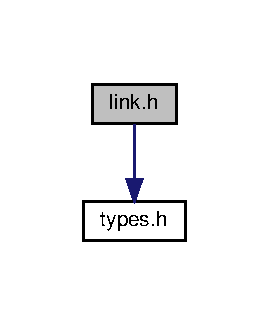
\includegraphics[width=172pt]{link_8h__incl}
\end{center}
\end{figure}
This graph shows which files directly or indirectly include this file\+:
\nopagebreak
\begin{figure}[H]
\begin{center}
\leavevmode
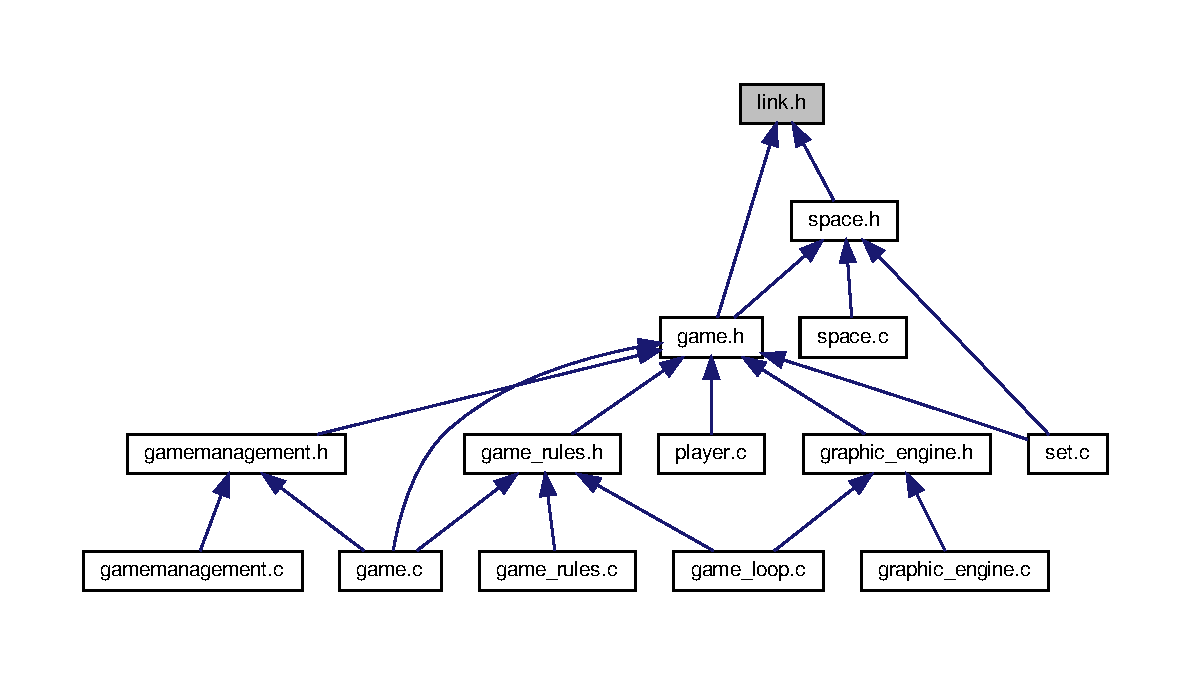
\includegraphics[width=350pt]{link_8h__dep__incl}
\end{center}
\end{figure}
\subsection*{Macros}
\begin{DoxyCompactItemize}
\item 
\#define \hyperlink{link_8h_a660ed1ec8604982002a0d6eced0e0367}{M\+A\+X\+\_\+\+L\+I\+N\+K\+S}~35
\item 
\#define \hyperlink{link_8h_a4afa5d7ec0095eb4bc86093f4139e86e}{F\+I\+R\+S\+T\+\_\+\+L\+I\+N\+K}~1
\end{DoxyCompactItemize}
\subsection*{Typedefs}
\begin{DoxyCompactItemize}
\item 
\hypertarget{link_8h_ae3b299941e67be6971bfd64a25505eff}{typedef struct \hyperlink{struct__Link}{\+\_\+\+Link} \hyperlink{link_8h_ae3b299941e67be6971bfd64a25505eff}{Link}}\label{link_8h_ae3b299941e67be6971bfd64a25505eff}

\begin{DoxyCompactList}\small\item\em Estructura del link. \end{DoxyCompactList}\end{DoxyCompactItemize}
\subsection*{Functions}
\begin{DoxyCompactItemize}
\item 
\hyperlink{link_8h_ae3b299941e67be6971bfd64a25505eff}{Link} $\ast$ \hyperlink{link_8h_a8090d7f529cfd6a2fc5df3dd379fe514}{link\+\_\+create} (\hyperlink{types_8h_a845e604fb28f7e3d97549da3448149d3}{Id} id)
\begin{DoxyCompactList}\small\item\em Funcion que inicializa el link Funcion encargada de reservar espacio para el link e inizializar sus parametros. \end{DoxyCompactList}\item 
\hyperlink{types_8h_a32c27cc471df37f4fc818d65de0a56c4}{S\+T\+A\+T\+U\+S} \hyperlink{link_8h_a85c4dd77887bf31f651ea1162144d712}{link\+\_\+destroy} (\hyperlink{link_8h_ae3b299941e67be6971bfd64a25505eff}{Link} $\ast$link)
\begin{DoxyCompactList}\small\item\em Funcion encargada de liberar la memoria reservada para el link. \end{DoxyCompactList}\item 
\hyperlink{types_8h_a32c27cc471df37f4fc818d65de0a56c4}{S\+T\+A\+T\+U\+S} \hyperlink{link_8h_a6c7a3bd7a856288c377edbcd045912e6}{link\+\_\+set\+\_\+name} (\hyperlink{link_8h_ae3b299941e67be6971bfd64a25505eff}{Link} $\ast$link, char $\ast$name)
\begin{DoxyCompactList}\small\item\em Funcion encargada de cambiar el nombre del link. \end{DoxyCompactList}\item 
\hyperlink{types_8h_a32c27cc471df37f4fc818d65de0a56c4}{S\+T\+A\+T\+U\+S} \hyperlink{link_8h_a052f6c7d44c2aca8cf0fb6522d3aa8f5}{link\+\_\+set\+\_\+link} (\hyperlink{link_8h_ae3b299941e67be6971bfd64a25505eff}{Link} $\ast$link, \hyperlink{types_8h_a845e604fb28f7e3d97549da3448149d3}{Id} space1, \hyperlink{types_8h_a845e604fb28f7e3d97549da3448149d3}{Id} space2)
\begin{DoxyCompactList}\small\item\em Funcion encargada de conectar dos espacios con un link. \end{DoxyCompactList}\item 
\hyperlink{types_8h_a32c27cc471df37f4fc818d65de0a56c4}{S\+T\+A\+T\+U\+S} \hyperlink{link_8h_a53fb7b3753a6d8318a97721e1009184a}{link\+\_\+set\+\_\+status} (\hyperlink{link_8h_ae3b299941e67be6971bfd64a25505eff}{Link} $\ast$link, \hyperlink{types_8h_a4eb959f56c9de4fb79f4891902033093}{D\+O\+O\+R} status)
\begin{DoxyCompactList}\small\item\em Funcion encargada de cambiar el estado de la puerta del link. \end{DoxyCompactList}\item 
\hyperlink{types_8h_a845e604fb28f7e3d97549da3448149d3}{Id} \hyperlink{link_8h_a2bbd320f995a72b2ea7ea639b1c81892}{link\+\_\+get\+\_\+id} (\hyperlink{link_8h_ae3b299941e67be6971bfd64a25505eff}{Link} $\ast$link)
\begin{DoxyCompactList}\small\item\em Funcion encargada de darnos el id del link. \end{DoxyCompactList}\item 
char $\ast$ \hyperlink{link_8h_a9747ee8201a323e112e67bdeacbc90d8}{link\+\_\+get\+\_\+name} (\hyperlink{link_8h_ae3b299941e67be6971bfd64a25505eff}{Link} $\ast$link)
\begin{DoxyCompactList}\small\item\em Funcion que devuelve el nombre del link. \end{DoxyCompactList}\item 
\hyperlink{types_8h_a4eb959f56c9de4fb79f4891902033093}{D\+O\+O\+R} \hyperlink{link_8h_a62be17829072b49416e1b31a4165522a}{link\+\_\+get\+\_\+status} (\hyperlink{link_8h_ae3b299941e67be6971bfd64a25505eff}{Link} $\ast$link)
\begin{DoxyCompactList}\small\item\em Funcion encargada devolver el estado de la puerta. \end{DoxyCompactList}\item 
\hyperlink{types_8h_a845e604fb28f7e3d97549da3448149d3}{Id} $\ast$ \hyperlink{link_8h_aa70e419787ae9cdc7e67fcb6a6594bdf}{link\+\_\+get\+\_\+link} (\hyperlink{link_8h_ae3b299941e67be6971bfd64a25505eff}{Link} $\ast$link)
\begin{DoxyCompactList}\small\item\em Funcion encargada devolver los ids de los espacios que forman el link. \end{DoxyCompactList}\item 
size\+\_\+t \hyperlink{link_8h_a25ae7fce6d0a05cb6f34c414ce5f8879}{link\+\_\+get\+\_\+size} ()
\begin{DoxyCompactList}\small\item\em Funcion encargada devolver el tamaño del link en memoria. \end{DoxyCompactList}\item 
\hyperlink{types_8h_a845e604fb28f7e3d97549da3448149d3}{Id} \hyperlink{link_8h_a4da473a85ef32634d63a56498f9a156f}{link\+\_\+space\+\_\+connected\+\_\+to} (\hyperlink{link_8h_ae3b299941e67be6971bfd64a25505eff}{Link} $\ast$link, \hyperlink{types_8h_a845e604fb28f7e3d97549da3448149d3}{Id} space)
\begin{DoxyCompactList}\small\item\em Funcion encargada devolver el espacio al que esta conectado otro espacio con ese link. \end{DoxyCompactList}\item 
\hyperlink{types_8h_a32c27cc471df37f4fc818d65de0a56c4}{S\+T\+A\+T\+U\+S} \hyperlink{link_8h_a95ea756dad592e65440a33dfbe47edcf}{link\+\_\+print} (\hyperlink{link_8h_ae3b299941e67be6971bfd64a25505eff}{Link} $\ast$link)
\begin{DoxyCompactList}\small\item\em Funcion encargada de imprimir el link. \end{DoxyCompactList}\end{DoxyCompactItemize}


\subsection{Detailed Description}
It implements the link interpreter. 

\begin{DoxyAuthor}{Author}
Sergio de los Reyes 
\end{DoxyAuthor}
\begin{DoxyVersion}{Version}
1.\+0 
\end{DoxyVersion}
\begin{DoxyDate}{Date}
08/03/2018 
\end{DoxyDate}


\subsection{Macro Definition Documentation}
\hypertarget{link_8h_a4afa5d7ec0095eb4bc86093f4139e86e}{\index{link.\+h@{link.\+h}!F\+I\+R\+S\+T\+\_\+\+L\+I\+N\+K@{F\+I\+R\+S\+T\+\_\+\+L\+I\+N\+K}}
\index{F\+I\+R\+S\+T\+\_\+\+L\+I\+N\+K@{F\+I\+R\+S\+T\+\_\+\+L\+I\+N\+K}!link.\+h@{link.\+h}}
\subsubsection[{F\+I\+R\+S\+T\+\_\+\+L\+I\+N\+K}]{\setlength{\rightskip}{0pt plus 5cm}\#define F\+I\+R\+S\+T\+\_\+\+L\+I\+N\+K~1}}\label{link_8h_a4afa5d7ec0095eb4bc86093f4139e86e}
Identificador del primer link \hypertarget{link_8h_a660ed1ec8604982002a0d6eced0e0367}{\index{link.\+h@{link.\+h}!M\+A\+X\+\_\+\+L\+I\+N\+K\+S@{M\+A\+X\+\_\+\+L\+I\+N\+K\+S}}
\index{M\+A\+X\+\_\+\+L\+I\+N\+K\+S@{M\+A\+X\+\_\+\+L\+I\+N\+K\+S}!link.\+h@{link.\+h}}
\subsubsection[{M\+A\+X\+\_\+\+L\+I\+N\+K\+S}]{\setlength{\rightskip}{0pt plus 5cm}\#define M\+A\+X\+\_\+\+L\+I\+N\+K\+S~35}}\label{link_8h_a660ed1ec8604982002a0d6eced0e0367}
Número máximo de links 

\subsection{Function Documentation}
\hypertarget{link_8h_a8090d7f529cfd6a2fc5df3dd379fe514}{\index{link.\+h@{link.\+h}!link\+\_\+create@{link\+\_\+create}}
\index{link\+\_\+create@{link\+\_\+create}!link.\+h@{link.\+h}}
\subsubsection[{link\+\_\+create}]{\setlength{\rightskip}{0pt plus 5cm}{\bf Link}$\ast$ link\+\_\+create (
\begin{DoxyParamCaption}
\item[{{\bf Id}}]{id}
\end{DoxyParamCaption}
)}}\label{link_8h_a8090d7f529cfd6a2fc5df3dd379fe514}


Funcion que inicializa el link Funcion encargada de reservar espacio para el link e inizializar sus parametros. 

\begin{DoxyAuthor}{Author}
Sergio de los Reyes 
\end{DoxyAuthor}

\begin{DoxyParams}{Parameters}
{\em id} & se corresponde con el id del link \\
\hline
\end{DoxyParams}
\begin{DoxyReturn}{Returns}
El link creado 
\end{DoxyReturn}
\hypertarget{link_8h_a85c4dd77887bf31f651ea1162144d712}{\index{link.\+h@{link.\+h}!link\+\_\+destroy@{link\+\_\+destroy}}
\index{link\+\_\+destroy@{link\+\_\+destroy}!link.\+h@{link.\+h}}
\subsubsection[{link\+\_\+destroy}]{\setlength{\rightskip}{0pt plus 5cm}{\bf S\+T\+A\+T\+U\+S} link\+\_\+destroy (
\begin{DoxyParamCaption}
\item[{{\bf Link} $\ast$}]{link}
\end{DoxyParamCaption}
)}}\label{link_8h_a85c4dd77887bf31f651ea1162144d712}


Funcion encargada de liberar la memoria reservada para el link. 

\begin{DoxyAuthor}{Author}
Sergio de los Reyes 
\end{DoxyAuthor}

\begin{DoxyParams}{Parameters}
{\em link} & link a destruir \\
\hline
\end{DoxyParams}
\begin{DoxyReturn}{Returns}
si se ha hecho o no correctamente 
\end{DoxyReturn}
\hypertarget{link_8h_a2bbd320f995a72b2ea7ea639b1c81892}{\index{link.\+h@{link.\+h}!link\+\_\+get\+\_\+id@{link\+\_\+get\+\_\+id}}
\index{link\+\_\+get\+\_\+id@{link\+\_\+get\+\_\+id}!link.\+h@{link.\+h}}
\subsubsection[{link\+\_\+get\+\_\+id}]{\setlength{\rightskip}{0pt plus 5cm}{\bf Id} link\+\_\+get\+\_\+id (
\begin{DoxyParamCaption}
\item[{{\bf Link} $\ast$}]{link}
\end{DoxyParamCaption}
)}}\label{link_8h_a2bbd320f995a72b2ea7ea639b1c81892}


Funcion encargada de darnos el id del link. 

\begin{DoxyAuthor}{Author}
Sergio de los Reyes 
\end{DoxyAuthor}

\begin{DoxyParams}{Parameters}
{\em link} & link \\
\hline
\end{DoxyParams}
\begin{DoxyReturn}{Returns}
id del link 
\end{DoxyReturn}
\hypertarget{link_8h_aa70e419787ae9cdc7e67fcb6a6594bdf}{\index{link.\+h@{link.\+h}!link\+\_\+get\+\_\+link@{link\+\_\+get\+\_\+link}}
\index{link\+\_\+get\+\_\+link@{link\+\_\+get\+\_\+link}!link.\+h@{link.\+h}}
\subsubsection[{link\+\_\+get\+\_\+link}]{\setlength{\rightskip}{0pt plus 5cm}{\bf Id}$\ast$ link\+\_\+get\+\_\+link (
\begin{DoxyParamCaption}
\item[{{\bf Link} $\ast$}]{link}
\end{DoxyParamCaption}
)}}\label{link_8h_aa70e419787ae9cdc7e67fcb6a6594bdf}


Funcion encargada devolver los ids de los espacios que forman el link. 

\begin{DoxyAuthor}{Author}
Sergio de los Reyes 
\end{DoxyAuthor}

\begin{DoxyParams}{Parameters}
{\em link} & link \\
\hline
\end{DoxyParams}
\begin{DoxyReturn}{Returns}
array de 2 ids con los ids de los espacios del link 
\end{DoxyReturn}
\hypertarget{link_8h_a9747ee8201a323e112e67bdeacbc90d8}{\index{link.\+h@{link.\+h}!link\+\_\+get\+\_\+name@{link\+\_\+get\+\_\+name}}
\index{link\+\_\+get\+\_\+name@{link\+\_\+get\+\_\+name}!link.\+h@{link.\+h}}
\subsubsection[{link\+\_\+get\+\_\+name}]{\setlength{\rightskip}{0pt plus 5cm}char$\ast$ link\+\_\+get\+\_\+name (
\begin{DoxyParamCaption}
\item[{{\bf Link} $\ast$}]{link}
\end{DoxyParamCaption}
)}}\label{link_8h_a9747ee8201a323e112e67bdeacbc90d8}


Funcion que devuelve el nombre del link. 

\begin{DoxyAuthor}{Author}
Sergio de los Reyes 
\end{DoxyAuthor}

\begin{DoxyParams}{Parameters}
{\em link} & link \\
\hline
\end{DoxyParams}
\begin{DoxyReturn}{Returns}
nombre del link 
\end{DoxyReturn}
\hypertarget{link_8h_a25ae7fce6d0a05cb6f34c414ce5f8879}{\index{link.\+h@{link.\+h}!link\+\_\+get\+\_\+size@{link\+\_\+get\+\_\+size}}
\index{link\+\_\+get\+\_\+size@{link\+\_\+get\+\_\+size}!link.\+h@{link.\+h}}
\subsubsection[{link\+\_\+get\+\_\+size}]{\setlength{\rightskip}{0pt plus 5cm}size\+\_\+t link\+\_\+get\+\_\+size (
\begin{DoxyParamCaption}
{}
\end{DoxyParamCaption}
)}}\label{link_8h_a25ae7fce6d0a05cb6f34c414ce5f8879}


Funcion encargada devolver el tamaño del link en memoria. 

\begin{DoxyAuthor}{Author}
Julia Simon 
\end{DoxyAuthor}
\begin{DoxyReturn}{Returns}
tamaño 
\end{DoxyReturn}
\hypertarget{link_8h_a62be17829072b49416e1b31a4165522a}{\index{link.\+h@{link.\+h}!link\+\_\+get\+\_\+status@{link\+\_\+get\+\_\+status}}
\index{link\+\_\+get\+\_\+status@{link\+\_\+get\+\_\+status}!link.\+h@{link.\+h}}
\subsubsection[{link\+\_\+get\+\_\+status}]{\setlength{\rightskip}{0pt plus 5cm}{\bf D\+O\+O\+R} link\+\_\+get\+\_\+status (
\begin{DoxyParamCaption}
\item[{{\bf Link} $\ast$}]{link}
\end{DoxyParamCaption}
)}}\label{link_8h_a62be17829072b49416e1b31a4165522a}


Funcion encargada devolver el estado de la puerta. 

\begin{DoxyAuthor}{Author}
Sergio de los Reyes 
\end{DoxyAuthor}

\begin{DoxyParams}{Parameters}
{\em link} & link \\
\hline
\end{DoxyParams}
\begin{DoxyReturn}{Returns}
si se ha hecho o no correctamente 
\end{DoxyReturn}
\hypertarget{link_8h_a95ea756dad592e65440a33dfbe47edcf}{\index{link.\+h@{link.\+h}!link\+\_\+print@{link\+\_\+print}}
\index{link\+\_\+print@{link\+\_\+print}!link.\+h@{link.\+h}}
\subsubsection[{link\+\_\+print}]{\setlength{\rightskip}{0pt plus 5cm}{\bf S\+T\+A\+T\+U\+S} link\+\_\+print (
\begin{DoxyParamCaption}
\item[{{\bf Link} $\ast$}]{link}
\end{DoxyParamCaption}
)}}\label{link_8h_a95ea756dad592e65440a33dfbe47edcf}


Funcion encargada de imprimir el link. 

\begin{DoxyAuthor}{Author}
Sergio de los Reyes 
\end{DoxyAuthor}

\begin{DoxyParams}{Parameters}
{\em link} & link \\
\hline
\end{DoxyParams}
\begin{DoxyReturn}{Returns}
si se ha hecho o no correctamente 
\end{DoxyReturn}
\hypertarget{link_8h_a052f6c7d44c2aca8cf0fb6522d3aa8f5}{\index{link.\+h@{link.\+h}!link\+\_\+set\+\_\+link@{link\+\_\+set\+\_\+link}}
\index{link\+\_\+set\+\_\+link@{link\+\_\+set\+\_\+link}!link.\+h@{link.\+h}}
\subsubsection[{link\+\_\+set\+\_\+link}]{\setlength{\rightskip}{0pt plus 5cm}{\bf S\+T\+A\+T\+U\+S} link\+\_\+set\+\_\+link (
\begin{DoxyParamCaption}
\item[{{\bf Link} $\ast$}]{link, }
\item[{{\bf Id}}]{space1, }
\item[{{\bf Id}}]{space2}
\end{DoxyParamCaption}
)}}\label{link_8h_a052f6c7d44c2aca8cf0fb6522d3aa8f5}


Funcion encargada de conectar dos espacios con un link. 

\begin{DoxyAuthor}{Author}
Sergio de los Reyes 
\end{DoxyAuthor}

\begin{DoxyParams}{Parameters}
{\em link} & link \\
\hline
{\em space1} & id del primer espacio \\
\hline
{\em space2} & id del segundo espacio \\
\hline
\end{DoxyParams}
\begin{DoxyReturn}{Returns}
si se ha hecho o no correctamente 
\end{DoxyReturn}
\hypertarget{link_8h_a6c7a3bd7a856288c377edbcd045912e6}{\index{link.\+h@{link.\+h}!link\+\_\+set\+\_\+name@{link\+\_\+set\+\_\+name}}
\index{link\+\_\+set\+\_\+name@{link\+\_\+set\+\_\+name}!link.\+h@{link.\+h}}
\subsubsection[{link\+\_\+set\+\_\+name}]{\setlength{\rightskip}{0pt plus 5cm}{\bf S\+T\+A\+T\+U\+S} link\+\_\+set\+\_\+name (
\begin{DoxyParamCaption}
\item[{{\bf Link} $\ast$}]{link, }
\item[{char $\ast$}]{name}
\end{DoxyParamCaption}
)}}\label{link_8h_a6c7a3bd7a856288c377edbcd045912e6}


Funcion encargada de cambiar el nombre del link. 

\begin{DoxyAuthor}{Author}
Sergio de los Reyes 
\end{DoxyAuthor}

\begin{DoxyParams}{Parameters}
{\em link} & link \\
\hline
{\em name} & nombre del link \\
\hline
\end{DoxyParams}
\begin{DoxyReturn}{Returns}
si se ha hecho o no correctamente 
\end{DoxyReturn}
\hypertarget{link_8h_a53fb7b3753a6d8318a97721e1009184a}{\index{link.\+h@{link.\+h}!link\+\_\+set\+\_\+status@{link\+\_\+set\+\_\+status}}
\index{link\+\_\+set\+\_\+status@{link\+\_\+set\+\_\+status}!link.\+h@{link.\+h}}
\subsubsection[{link\+\_\+set\+\_\+status}]{\setlength{\rightskip}{0pt plus 5cm}{\bf S\+T\+A\+T\+U\+S} link\+\_\+set\+\_\+status (
\begin{DoxyParamCaption}
\item[{{\bf Link} $\ast$}]{link, }
\item[{{\bf D\+O\+O\+R}}]{status}
\end{DoxyParamCaption}
)}}\label{link_8h_a53fb7b3753a6d8318a97721e1009184a}


Funcion encargada de cambiar el estado de la puerta del link. 

\begin{DoxyAuthor}{Author}
Sergio de los Reyes 
\end{DoxyAuthor}

\begin{DoxyParams}{Parameters}
{\em link} & link \\
\hline
{\em status} & estado de la puerta (abierto o cerrado) \\
\hline
\end{DoxyParams}
\begin{DoxyReturn}{Returns}
si se ha hecho o no correctamente 
\end{DoxyReturn}
\hypertarget{link_8h_a4da473a85ef32634d63a56498f9a156f}{\index{link.\+h@{link.\+h}!link\+\_\+space\+\_\+connected\+\_\+to@{link\+\_\+space\+\_\+connected\+\_\+to}}
\index{link\+\_\+space\+\_\+connected\+\_\+to@{link\+\_\+space\+\_\+connected\+\_\+to}!link.\+h@{link.\+h}}
\subsubsection[{link\+\_\+space\+\_\+connected\+\_\+to}]{\setlength{\rightskip}{0pt plus 5cm}{\bf Id} link\+\_\+space\+\_\+connected\+\_\+to (
\begin{DoxyParamCaption}
\item[{{\bf Link} $\ast$}]{link, }
\item[{{\bf Id}}]{space}
\end{DoxyParamCaption}
)}}\label{link_8h_a4da473a85ef32634d63a56498f9a156f}


Funcion encargada devolver el espacio al que esta conectado otro espacio con ese link. 

\begin{DoxyAuthor}{Author}
Sergio de los Reyes 
\end{DoxyAuthor}

\begin{DoxyParams}{Parameters}
{\em link} & link \\
\hline
{\em space} & espacio del que queremos buscar a cual se conecta \\
\hline
\end{DoxyParams}
\begin{DoxyReturn}{Returns}
id del espacio al que esta conectado space 
\end{DoxyReturn}

\hypertarget{object_8h}{\section{include/object.h File Reference}
\label{object_8h}\index{include/object.\+h@{include/object.\+h}}
}


It defines a object.  


{\ttfamily \#include \char`\"{}../include/types.\+h\char`\"{}}\\*
Include dependency graph for object.\+h\+:
\nopagebreak
\begin{figure}[H]
\begin{center}
\leavevmode
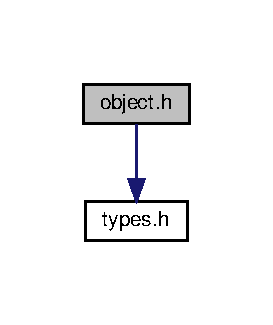
\includegraphics[width=172pt]{object_8h__incl}
\end{center}
\end{figure}
This graph shows which files directly or indirectly include this file\+:
\nopagebreak
\begin{figure}[H]
\begin{center}
\leavevmode
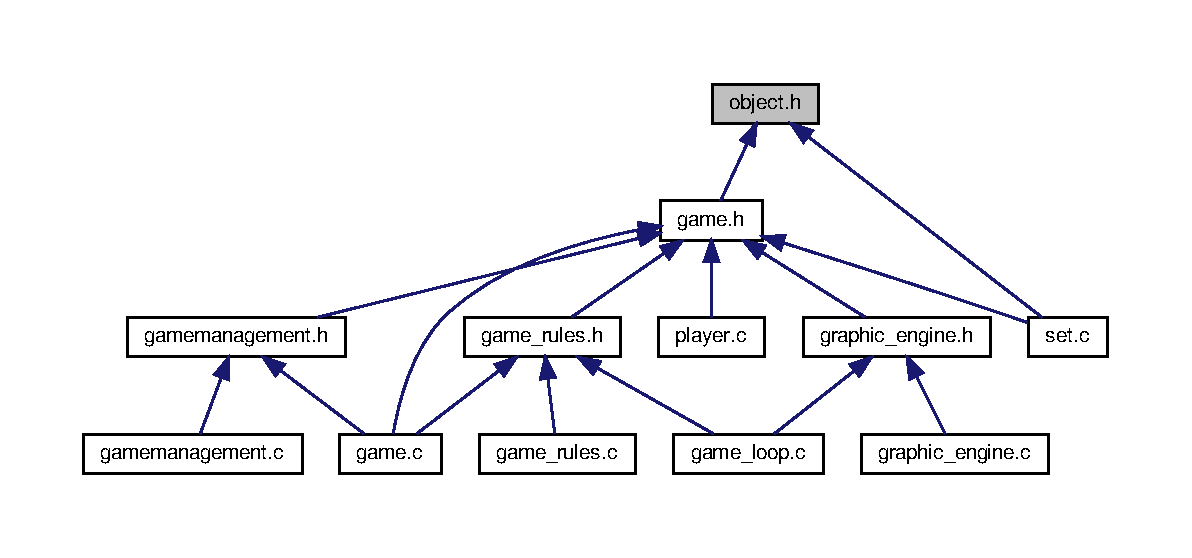
\includegraphics[width=350pt]{object_8h__dep__incl}
\end{center}
\end{figure}
\subsection*{Macros}
\begin{DoxyCompactItemize}
\item 
\#define \hyperlink{object_8h_acdc7844fbd4d45737d4aa56834d37829}{M\+A\+X\+\_\+\+O\+B\+J\+E\+C\+T\+S}~100
\end{DoxyCompactItemize}
\subsection*{Typedefs}
\begin{DoxyCompactItemize}
\item 
\hypertarget{object_8h_a7f8bbcda919b65ce67f92fba08e0212f}{typedef struct \hyperlink{struct__Object}{\+\_\+\+Object} \hyperlink{object_8h_a7f8bbcda919b65ce67f92fba08e0212f}{Object}}\label{object_8h_a7f8bbcda919b65ce67f92fba08e0212f}

\begin{DoxyCompactList}\small\item\em Estructura del objeto. \end{DoxyCompactList}\end{DoxyCompactItemize}
\subsection*{Functions}
\begin{DoxyCompactItemize}
\item 
\hyperlink{object_8h_a7f8bbcda919b65ce67f92fba08e0212f}{Object} $\ast$ \hyperlink{object_8h_abb0cd30fca5fbddf137c6c04df66bbc7}{object\+\_\+create} (\hyperlink{types_8h_a845e604fb28f7e3d97549da3448149d3}{Id} id)
\begin{DoxyCompactList}\small\item\em Funcion encargada de reservar memoria para un objeto. \end{DoxyCompactList}\item 
\hyperlink{types_8h_a32c27cc471df37f4fc818d65de0a56c4}{S\+T\+A\+T\+U\+S} \hyperlink{object_8h_a19d6d51fee809e3801893eefc789f4b4}{object\+\_\+destroy} (\hyperlink{object_8h_a7f8bbcda919b65ce67f92fba08e0212f}{Object} $\ast$object)
\begin{DoxyCompactList}\small\item\em Funcion encargada de liberar la memoria reservada para el objeto. \end{DoxyCompactList}\item 
\hyperlink{types_8h_a32c27cc471df37f4fc818d65de0a56c4}{S\+T\+A\+T\+U\+S} \hyperlink{object_8h_ac15dc062c857503ec0ca66037caffd80}{object\+\_\+set\+\_\+name} (\hyperlink{object_8h_a7f8bbcda919b65ce67f92fba08e0212f}{Object} $\ast$object, char $\ast$name)
\begin{DoxyCompactList}\small\item\em Funcion encargada de cambiar el nombre de un objeto. \end{DoxyCompactList}\item 
\hyperlink{types_8h_a32c27cc471df37f4fc818d65de0a56c4}{S\+T\+A\+T\+U\+S} \hyperlink{object_8h_a352bd939c515fd5e3baee189ddaa606a}{object\+\_\+set\+\_\+description} (\hyperlink{object_8h_a7f8bbcda919b65ce67f92fba08e0212f}{Object} $\ast$object, char $\ast$string)
\begin{DoxyCompactList}\small\item\em Funcion encargada de cambiar la descripción del objeto. \end{DoxyCompactList}\item 
\hyperlink{types_8h_a32c27cc471df37f4fc818d65de0a56c4}{S\+T\+A\+T\+U\+S} \hyperlink{object_8h_a279df1e8d8473c787bfce7072a6a6f2a}{object\+\_\+set\+\_\+des\+\_\+movido} (\hyperlink{object_8h_a7f8bbcda919b65ce67f92fba08e0212f}{Object} $\ast$object)
\begin{DoxyCompactList}\small\item\em Funcion encargada de cambiar la descripción del objeto cuando ha sido movido. \end{DoxyCompactList}\item 
\hyperlink{types_8h_a32c27cc471df37f4fc818d65de0a56c4}{S\+T\+A\+T\+U\+S} \hyperlink{object_8h_ae95a1ce5479928e05d85f6b5fa2871c0}{object\+\_\+set\+\_\+pos\+\_\+inicial} (\hyperlink{object_8h_a7f8bbcda919b65ce67f92fba08e0212f}{Object} $\ast$object, \hyperlink{types_8h_a845e604fb28f7e3d97549da3448149d3}{Id} space)
\begin{DoxyCompactList}\small\item\em Funcion que guarda la posicion inicial del objeto. \end{DoxyCompactList}\item 
\hyperlink{types_8h_a845e604fb28f7e3d97549da3448149d3}{Id} \hyperlink{object_8h_ac5af152381a21853c6a28cc120e8e7fe}{object\+\_\+get\+\_\+id} (\hyperlink{object_8h_a7f8bbcda919b65ce67f92fba08e0212f}{Object} $\ast$object)
\begin{DoxyCompactList}\small\item\em Funcion encargada de decirnos el id del objeto. \end{DoxyCompactList}\item 
char $\ast$ \hyperlink{object_8h_a7954dbdd53d8b5dc259993f04bba28f8}{object\+\_\+get\+\_\+name} (\hyperlink{object_8h_a7f8bbcda919b65ce67f92fba08e0212f}{Object} $\ast$object)
\begin{DoxyCompactList}\small\item\em Funcion encargada de decirnos el nombre del objeto. \end{DoxyCompactList}\item 
char $\ast$ \hyperlink{object_8h_ab92f583fcb6e3000ebe48cc04c5853cd}{object\+\_\+get\+\_\+description} (\hyperlink{object_8h_a7f8bbcda919b65ce67f92fba08e0212f}{Object} $\ast$object)
\begin{DoxyCompactList}\small\item\em Funcion encargada de decirnos la descripción del objeto Nos devuelve una descripcion u otra en función de si ha sido o no movido respecto de su posicion original. \end{DoxyCompactList}\item 
\hyperlink{types_8h_a845e604fb28f7e3d97549da3448149d3}{Id} \hyperlink{object_8h_abe1f4e65fe87ea1e4c3bf4637e8273f0}{object\+\_\+get\+\_\+pos\+\_\+inicial} (\hyperlink{object_8h_a7f8bbcda919b65ce67f92fba08e0212f}{Object} $\ast$object)
\begin{DoxyCompactList}\small\item\em Funcion que devuelve la posicion inicial del objeto. \end{DoxyCompactList}\item 
\hyperlink{types_8h_a32c27cc471df37f4fc818d65de0a56c4}{S\+T\+A\+T\+U\+S} \hyperlink{object_8h_adebb77fb5d33fc70616ab3b2b64c27ce}{object\+\_\+print} (\hyperlink{object_8h_a7f8bbcda919b65ce67f92fba08e0212f}{Object} $\ast$object)
\begin{DoxyCompactList}\small\item\em Funcion encargada de darnos toda la informacion de un objeto. \end{DoxyCompactList}\item 
\hyperlink{types_8h_a3e5b8192e7d9ffaf3542f1210aec18dd}{B\+O\+O\+L} \hyperlink{object_8h_aa16dfdded78cfb67cf4b9bcd425f199a}{object\+\_\+get\+\_\+movible} (\hyperlink{object_8h_a7f8bbcda919b65ce67f92fba08e0212f}{Object} $\ast$object)
\begin{DoxyCompactList}\small\item\em Devuelve la movilidad del objeto Es decir, indica si el objeto se va a poder mover o no de su posicion inicial. \end{DoxyCompactList}\item 
\hyperlink{types_8h_a32c27cc471df37f4fc818d65de0a56c4}{S\+T\+A\+T\+U\+S} \hyperlink{object_8h_ab67660a09c514d65452fb4a4fa7ec493}{object\+\_\+set\+\_\+movible} (\hyperlink{object_8h_a7f8bbcda919b65ce67f92fba08e0212f}{Object} $\ast$object, \hyperlink{types_8h_a3e5b8192e7d9ffaf3542f1210aec18dd}{B\+O\+O\+L} movible)
\begin{DoxyCompactList}\small\item\em Establece la movilidad del objeto. \end{DoxyCompactList}\item 
\hyperlink{types_8h_a3e5b8192e7d9ffaf3542f1210aec18dd}{B\+O\+O\+L} \hyperlink{object_8h_adf2cba90c6b63690720a094cfe8fbf19}{object\+\_\+get\+\_\+movido} (\hyperlink{object_8h_a7f8bbcda919b65ce67f92fba08e0212f}{Object} $\ast$object)
\begin{DoxyCompactList}\small\item\em Devuelve si el objeto se ha movido. \end{DoxyCompactList}\item 
\hyperlink{types_8h_a32c27cc471df37f4fc818d65de0a56c4}{S\+T\+A\+T\+U\+S} \hyperlink{object_8h_a577d445a84a1f60cc7c756a3e9a00e74}{object\+\_\+set\+\_\+movido} (\hyperlink{object_8h_a7f8bbcda919b65ce67f92fba08e0212f}{Object} $\ast$object, \hyperlink{types_8h_a3e5b8192e7d9ffaf3542f1210aec18dd}{B\+O\+O\+L} movido)
\begin{DoxyCompactList}\small\item\em Establece si el objeto se ha movido. \end{DoxyCompactList}\item 
\hyperlink{types_8h_a3e5b8192e7d9ffaf3542f1210aec18dd}{B\+O\+O\+L} \hyperlink{object_8h_a9e49f66ecc1c29e5eb83c5915814e2b4}{object\+\_\+get\+\_\+oculto} (\hyperlink{object_8h_a7f8bbcda919b65ce67f92fba08e0212f}{Object} $\ast$object)
\begin{DoxyCompactList}\small\item\em Devuelve si el objeto esta oculto. \end{DoxyCompactList}\item 
\hyperlink{types_8h_a32c27cc471df37f4fc818d65de0a56c4}{S\+T\+A\+T\+U\+S} \hyperlink{object_8h_aa370f8431dc57329b1c561a033e198bd}{object\+\_\+set\+\_\+oculto} (\hyperlink{object_8h_a7f8bbcda919b65ce67f92fba08e0212f}{Object} $\ast$object, \hyperlink{types_8h_a3e5b8192e7d9ffaf3542f1210aec18dd}{B\+O\+O\+L} oculto)
\begin{DoxyCompactList}\small\item\em Establece la visibilidad del objetp. \end{DoxyCompactList}\item 
\hyperlink{types_8h_a845e604fb28f7e3d97549da3448149d3}{Id} \hyperlink{object_8h_a49dbce205db36230c53fb0ccf0a73174}{object\+\_\+get\+\_\+open} (\hyperlink{object_8h_a7f8bbcda919b65ce67f92fba08e0212f}{Object} $\ast$object)
\begin{DoxyCompactList}\small\item\em Devuelve el id del link que abre. \end{DoxyCompactList}\item 
\hyperlink{types_8h_a32c27cc471df37f4fc818d65de0a56c4}{S\+T\+A\+T\+U\+S} \hyperlink{object_8h_a3afab23d0ed66591693f1ecd8a85e0df}{object\+\_\+set\+\_\+open} (\hyperlink{object_8h_a7f8bbcda919b65ce67f92fba08e0212f}{Object} $\ast$object, \hyperlink{types_8h_a845e604fb28f7e3d97549da3448149d3}{Id} open)
\begin{DoxyCompactList}\small\item\em Establece que abre el objeto. \end{DoxyCompactList}\item 
\hyperlink{types_8h_a3e5b8192e7d9ffaf3542f1210aec18dd}{B\+O\+O\+L} \hyperlink{object_8h_aba5a8583a56db5cc0f861d6e8c48c1a7}{object\+\_\+get\+\_\+iluminado} (\hyperlink{object_8h_a7f8bbcda919b65ce67f92fba08e0212f}{Object} $\ast$object)
\begin{DoxyCompactList}\small\item\em Devuelve si el objeto esta ilumonado. \end{DoxyCompactList}\item 
\hyperlink{types_8h_a32c27cc471df37f4fc818d65de0a56c4}{S\+T\+A\+T\+U\+S} \hyperlink{object_8h_a61d2b95e4ee9a120ebdb049a0479d8f7}{object\+\_\+set\+\_\+iluminado} (\hyperlink{object_8h_a7f8bbcda919b65ce67f92fba08e0212f}{Object} $\ast$object, \hyperlink{types_8h_a3e5b8192e7d9ffaf3542f1210aec18dd}{B\+O\+O\+L} iluminado)
\begin{DoxyCompactList}\small\item\em Establece la iluminacion del objeto. \end{DoxyCompactList}\item 
\hyperlink{types_8h_a3e5b8192e7d9ffaf3542f1210aec18dd}{B\+O\+O\+L} \hyperlink{object_8h_a7aa4240bb16a17e130623f6ba88e57fd}{object\+\_\+get\+\_\+encendido} (\hyperlink{object_8h_a7f8bbcda919b65ce67f92fba08e0212f}{Object} $\ast$object)
\begin{DoxyCompactList}\small\item\em Devuelve si el objeto esta encendido. \end{DoxyCompactList}\item 
\hyperlink{types_8h_a32c27cc471df37f4fc818d65de0a56c4}{S\+T\+A\+T\+U\+S} \hyperlink{object_8h_a19ebfcfebe1618fbe000d5768f759557}{object\+\_\+set\+\_\+encendido} (\hyperlink{object_8h_a7f8bbcda919b65ce67f92fba08e0212f}{Object} $\ast$object, \hyperlink{types_8h_a3e5b8192e7d9ffaf3542f1210aec18dd}{B\+O\+O\+L} encendido)
\begin{DoxyCompactList}\small\item\em Establece si el objeto esta encendido. \end{DoxyCompactList}\item 
size\+\_\+t \hyperlink{object_8h_a7ee5148e5bbfa4fc0f81d94b4fea7c33}{object\+\_\+get\+\_\+size} ()
\begin{DoxyCompactList}\small\item\em Funcion encargada de darnos el tamaño del objeto en memoria. \end{DoxyCompactList}\end{DoxyCompactItemize}


\subsection{Detailed Description}
It defines a object. 

\begin{DoxyAuthor}{Author}
Julia Simon y Miguel Rodriguez 
\end{DoxyAuthor}
\begin{DoxyVersion}{Version}
1.\+0 
\end{DoxyVersion}
\begin{DoxyDate}{Date}
13-\/02-\/2018 
\end{DoxyDate}


\subsection{Macro Definition Documentation}
\hypertarget{object_8h_acdc7844fbd4d45737d4aa56834d37829}{\index{object.\+h@{object.\+h}!M\+A\+X\+\_\+\+O\+B\+J\+E\+C\+T\+S@{M\+A\+X\+\_\+\+O\+B\+J\+E\+C\+T\+S}}
\index{M\+A\+X\+\_\+\+O\+B\+J\+E\+C\+T\+S@{M\+A\+X\+\_\+\+O\+B\+J\+E\+C\+T\+S}!object.\+h@{object.\+h}}
\subsubsection[{M\+A\+X\+\_\+\+O\+B\+J\+E\+C\+T\+S}]{\setlength{\rightskip}{0pt plus 5cm}\#define M\+A\+X\+\_\+\+O\+B\+J\+E\+C\+T\+S~100}}\label{object_8h_acdc7844fbd4d45737d4aa56834d37829}
numero maximo de objetos 

\subsection{Function Documentation}
\hypertarget{object_8h_abb0cd30fca5fbddf137c6c04df66bbc7}{\index{object.\+h@{object.\+h}!object\+\_\+create@{object\+\_\+create}}
\index{object\+\_\+create@{object\+\_\+create}!object.\+h@{object.\+h}}
\subsubsection[{object\+\_\+create}]{\setlength{\rightskip}{0pt plus 5cm}{\bf Object}$\ast$ object\+\_\+create (
\begin{DoxyParamCaption}
\item[{{\bf Id}}]{id}
\end{DoxyParamCaption}
)}}\label{object_8h_abb0cd30fca5fbddf137c6c04df66bbc7}


Funcion encargada de reservar memoria para un objeto. 

\begin{DoxyAuthor}{Author}
Miguel Rodriguez 
\end{DoxyAuthor}

\begin{DoxyParams}{Parameters}
{\em Id} & id del objeto que se va a crear \\
\hline
\end{DoxyParams}
\begin{DoxyReturn}{Returns}
objeto que se ha creado 
\end{DoxyReturn}
\hypertarget{object_8h_a19d6d51fee809e3801893eefc789f4b4}{\index{object.\+h@{object.\+h}!object\+\_\+destroy@{object\+\_\+destroy}}
\index{object\+\_\+destroy@{object\+\_\+destroy}!object.\+h@{object.\+h}}
\subsubsection[{object\+\_\+destroy}]{\setlength{\rightskip}{0pt plus 5cm}{\bf S\+T\+A\+T\+U\+S} object\+\_\+destroy (
\begin{DoxyParamCaption}
\item[{{\bf Object} $\ast$}]{object}
\end{DoxyParamCaption}
)}}\label{object_8h_a19d6d51fee809e3801893eefc789f4b4}


Funcion encargada de liberar la memoria reservada para el objeto. 

\begin{DoxyAuthor}{Author}
Miguel Rodriguez 
\end{DoxyAuthor}

\begin{DoxyParams}{Parameters}
{\em object} & objecto que se va a liberar \\
\hline
\end{DoxyParams}
\begin{DoxyReturn}{Returns}
O\+K si se ha liberado la memoria correctamente y E\+R\+R\+O\+R en caso de error 
\end{DoxyReturn}
\hypertarget{object_8h_ab92f583fcb6e3000ebe48cc04c5853cd}{\index{object.\+h@{object.\+h}!object\+\_\+get\+\_\+description@{object\+\_\+get\+\_\+description}}
\index{object\+\_\+get\+\_\+description@{object\+\_\+get\+\_\+description}!object.\+h@{object.\+h}}
\subsubsection[{object\+\_\+get\+\_\+description}]{\setlength{\rightskip}{0pt plus 5cm}char$\ast$ object\+\_\+get\+\_\+description (
\begin{DoxyParamCaption}
\item[{{\bf Object} $\ast$}]{object}
\end{DoxyParamCaption}
)}}\label{object_8h_ab92f583fcb6e3000ebe48cc04c5853cd}


Funcion encargada de decirnos la descripción del objeto Nos devuelve una descripcion u otra en función de si ha sido o no movido respecto de su posicion original. 

\begin{DoxyAuthor}{Author}
Julia Simon 
\end{DoxyAuthor}

\begin{DoxyParams}{Parameters}
{\em object} & objeto del que se quiere saber la descripción \\
\hline
\end{DoxyParams}
\begin{DoxyReturn}{Returns}
descripcion del objeto 
\end{DoxyReturn}
\hypertarget{object_8h_a7aa4240bb16a17e130623f6ba88e57fd}{\index{object.\+h@{object.\+h}!object\+\_\+get\+\_\+encendido@{object\+\_\+get\+\_\+encendido}}
\index{object\+\_\+get\+\_\+encendido@{object\+\_\+get\+\_\+encendido}!object.\+h@{object.\+h}}
\subsubsection[{object\+\_\+get\+\_\+encendido}]{\setlength{\rightskip}{0pt plus 5cm}{\bf B\+O\+O\+L} object\+\_\+get\+\_\+encendido (
\begin{DoxyParamCaption}
\item[{{\bf Object} $\ast$}]{object}
\end{DoxyParamCaption}
)}}\label{object_8h_a7aa4240bb16a17e130623f6ba88e57fd}


Devuelve si el objeto esta encendido. 

\begin{DoxyAuthor}{Author}
Sergio de los Reyes 
\end{DoxyAuthor}

\begin{DoxyParams}{Parameters}
{\em object} & el objeto \\
\hline
\end{DoxyParams}
\begin{DoxyReturn}{Returns}
un booleano (B\+O\+O\+L)\+: si esta encendido 
\end{DoxyReturn}
\hypertarget{object_8h_ac5af152381a21853c6a28cc120e8e7fe}{\index{object.\+h@{object.\+h}!object\+\_\+get\+\_\+id@{object\+\_\+get\+\_\+id}}
\index{object\+\_\+get\+\_\+id@{object\+\_\+get\+\_\+id}!object.\+h@{object.\+h}}
\subsubsection[{object\+\_\+get\+\_\+id}]{\setlength{\rightskip}{0pt plus 5cm}{\bf Id} object\+\_\+get\+\_\+id (
\begin{DoxyParamCaption}
\item[{{\bf Object} $\ast$}]{object}
\end{DoxyParamCaption}
)}}\label{object_8h_ac5af152381a21853c6a28cc120e8e7fe}


Funcion encargada de decirnos el id del objeto. 

\begin{DoxyAuthor}{Author}
Miguel Rodriguez 
\end{DoxyAuthor}

\begin{DoxyParams}{Parameters}
{\em object} & objeto del que se quiere saber el id \\
\hline
\end{DoxyParams}
\begin{DoxyReturn}{Returns}
id del objeto 
\end{DoxyReturn}
\hypertarget{object_8h_aba5a8583a56db5cc0f861d6e8c48c1a7}{\index{object.\+h@{object.\+h}!object\+\_\+get\+\_\+iluminado@{object\+\_\+get\+\_\+iluminado}}
\index{object\+\_\+get\+\_\+iluminado@{object\+\_\+get\+\_\+iluminado}!object.\+h@{object.\+h}}
\subsubsection[{object\+\_\+get\+\_\+iluminado}]{\setlength{\rightskip}{0pt plus 5cm}{\bf B\+O\+O\+L} object\+\_\+get\+\_\+iluminado (
\begin{DoxyParamCaption}
\item[{{\bf Object} $\ast$}]{object}
\end{DoxyParamCaption}
)}}\label{object_8h_aba5a8583a56db5cc0f861d6e8c48c1a7}


Devuelve si el objeto esta ilumonado. 

\begin{DoxyAuthor}{Author}
Sergio de los Reyes 
\end{DoxyAuthor}

\begin{DoxyParams}{Parameters}
{\em object} & el objeto \\
\hline
\end{DoxyParams}
\begin{DoxyReturn}{Returns}
un booleano (B\+O\+O\+L)\+: si esta iluminado 
\end{DoxyReturn}
\hypertarget{object_8h_aa16dfdded78cfb67cf4b9bcd425f199a}{\index{object.\+h@{object.\+h}!object\+\_\+get\+\_\+movible@{object\+\_\+get\+\_\+movible}}
\index{object\+\_\+get\+\_\+movible@{object\+\_\+get\+\_\+movible}!object.\+h@{object.\+h}}
\subsubsection[{object\+\_\+get\+\_\+movible}]{\setlength{\rightskip}{0pt plus 5cm}{\bf B\+O\+O\+L} object\+\_\+get\+\_\+movible (
\begin{DoxyParamCaption}
\item[{{\bf Object} $\ast$}]{object}
\end{DoxyParamCaption}
)}}\label{object_8h_aa16dfdded78cfb67cf4b9bcd425f199a}


Devuelve la movilidad del objeto Es decir, indica si el objeto se va a poder mover o no de su posicion inicial. 

\begin{DoxyAuthor}{Author}
Sergio de los Reyes 
\end{DoxyAuthor}

\begin{DoxyParams}{Parameters}
{\em object} & el objeto \\
\hline
\end{DoxyParams}
\begin{DoxyReturn}{Returns}
un booleano (B\+O\+O\+L)\+: la movilidad 
\end{DoxyReturn}
\hypertarget{object_8h_adf2cba90c6b63690720a094cfe8fbf19}{\index{object.\+h@{object.\+h}!object\+\_\+get\+\_\+movido@{object\+\_\+get\+\_\+movido}}
\index{object\+\_\+get\+\_\+movido@{object\+\_\+get\+\_\+movido}!object.\+h@{object.\+h}}
\subsubsection[{object\+\_\+get\+\_\+movido}]{\setlength{\rightskip}{0pt plus 5cm}{\bf B\+O\+O\+L} object\+\_\+get\+\_\+movido (
\begin{DoxyParamCaption}
\item[{{\bf Object} $\ast$}]{object}
\end{DoxyParamCaption}
)}}\label{object_8h_adf2cba90c6b63690720a094cfe8fbf19}


Devuelve si el objeto se ha movido. 

\begin{DoxyAuthor}{Author}
Sergio de los Reyes 
\end{DoxyAuthor}

\begin{DoxyParams}{Parameters}
{\em object} & el objeto \\
\hline
\end{DoxyParams}
\begin{DoxyReturn}{Returns}
un booleano (B\+O\+O\+L)\+: si se ha movido 
\end{DoxyReturn}
\hypertarget{object_8h_a7954dbdd53d8b5dc259993f04bba28f8}{\index{object.\+h@{object.\+h}!object\+\_\+get\+\_\+name@{object\+\_\+get\+\_\+name}}
\index{object\+\_\+get\+\_\+name@{object\+\_\+get\+\_\+name}!object.\+h@{object.\+h}}
\subsubsection[{object\+\_\+get\+\_\+name}]{\setlength{\rightskip}{0pt plus 5cm}char$\ast$ object\+\_\+get\+\_\+name (
\begin{DoxyParamCaption}
\item[{{\bf Object} $\ast$}]{object}
\end{DoxyParamCaption}
)}}\label{object_8h_a7954dbdd53d8b5dc259993f04bba28f8}


Funcion encargada de decirnos el nombre del objeto. 

\begin{DoxyAuthor}{Author}
Miguel Rodriguez 
\end{DoxyAuthor}

\begin{DoxyParams}{Parameters}
{\em object} & objeto del que se quiere saber el nombre \\
\hline
\end{DoxyParams}
\begin{DoxyReturn}{Returns}
nombre del objeto 
\end{DoxyReturn}
\hypertarget{object_8h_a9e49f66ecc1c29e5eb83c5915814e2b4}{\index{object.\+h@{object.\+h}!object\+\_\+get\+\_\+oculto@{object\+\_\+get\+\_\+oculto}}
\index{object\+\_\+get\+\_\+oculto@{object\+\_\+get\+\_\+oculto}!object.\+h@{object.\+h}}
\subsubsection[{object\+\_\+get\+\_\+oculto}]{\setlength{\rightskip}{0pt plus 5cm}{\bf B\+O\+O\+L} object\+\_\+get\+\_\+oculto (
\begin{DoxyParamCaption}
\item[{{\bf Object} $\ast$}]{object}
\end{DoxyParamCaption}
)}}\label{object_8h_a9e49f66ecc1c29e5eb83c5915814e2b4}


Devuelve si el objeto esta oculto. 

\begin{DoxyAuthor}{Author}
Sergio de los Reyes 
\end{DoxyAuthor}

\begin{DoxyParams}{Parameters}
{\em object} & el objeto \\
\hline
\end{DoxyParams}
\begin{DoxyReturn}{Returns}
un booleano (B\+O\+O\+L)\+: si esta oculto 
\end{DoxyReturn}
\hypertarget{object_8h_a49dbce205db36230c53fb0ccf0a73174}{\index{object.\+h@{object.\+h}!object\+\_\+get\+\_\+open@{object\+\_\+get\+\_\+open}}
\index{object\+\_\+get\+\_\+open@{object\+\_\+get\+\_\+open}!object.\+h@{object.\+h}}
\subsubsection[{object\+\_\+get\+\_\+open}]{\setlength{\rightskip}{0pt plus 5cm}{\bf Id} object\+\_\+get\+\_\+open (
\begin{DoxyParamCaption}
\item[{{\bf Object} $\ast$}]{object}
\end{DoxyParamCaption}
)}}\label{object_8h_a49dbce205db36230c53fb0ccf0a73174}


Devuelve el id del link que abre. 

\begin{DoxyAuthor}{Author}
Sergio de los Reyes 
\end{DoxyAuthor}

\begin{DoxyParams}{Parameters}
{\em object} & el objeto \\
\hline
\end{DoxyParams}
\begin{DoxyReturn}{Returns}
un int(id)\+: id 
\end{DoxyReturn}
\hypertarget{object_8h_abe1f4e65fe87ea1e4c3bf4637e8273f0}{\index{object.\+h@{object.\+h}!object\+\_\+get\+\_\+pos\+\_\+inicial@{object\+\_\+get\+\_\+pos\+\_\+inicial}}
\index{object\+\_\+get\+\_\+pos\+\_\+inicial@{object\+\_\+get\+\_\+pos\+\_\+inicial}!object.\+h@{object.\+h}}
\subsubsection[{object\+\_\+get\+\_\+pos\+\_\+inicial}]{\setlength{\rightskip}{0pt plus 5cm}{\bf Id} object\+\_\+get\+\_\+pos\+\_\+inicial (
\begin{DoxyParamCaption}
\item[{{\bf Object} $\ast$}]{object}
\end{DoxyParamCaption}
)}}\label{object_8h_abe1f4e65fe87ea1e4c3bf4637e8273f0}


Funcion que devuelve la posicion inicial del objeto. 

\begin{DoxyAuthor}{Author}
Julia Simon 
\end{DoxyAuthor}

\begin{DoxyParams}{Parameters}
{\em object} & el objeto \\
\hline
\end{DoxyParams}
\begin{DoxyReturn}{Returns}
Id del espacio inicial 
\end{DoxyReturn}
\hypertarget{object_8h_a7ee5148e5bbfa4fc0f81d94b4fea7c33}{\index{object.\+h@{object.\+h}!object\+\_\+get\+\_\+size@{object\+\_\+get\+\_\+size}}
\index{object\+\_\+get\+\_\+size@{object\+\_\+get\+\_\+size}!object.\+h@{object.\+h}}
\subsubsection[{object\+\_\+get\+\_\+size}]{\setlength{\rightskip}{0pt plus 5cm}size\+\_\+t object\+\_\+get\+\_\+size (
\begin{DoxyParamCaption}
{}
\end{DoxyParamCaption}
)}}\label{object_8h_a7ee5148e5bbfa4fc0f81d94b4fea7c33}


Funcion encargada de darnos el tamaño del objeto en memoria. 

\begin{DoxyAuthor}{Author}
Julia Simon 
\end{DoxyAuthor}
\begin{DoxyReturn}{Returns}
tamaño 
\end{DoxyReturn}
\hypertarget{object_8h_adebb77fb5d33fc70616ab3b2b64c27ce}{\index{object.\+h@{object.\+h}!object\+\_\+print@{object\+\_\+print}}
\index{object\+\_\+print@{object\+\_\+print}!object.\+h@{object.\+h}}
\subsubsection[{object\+\_\+print}]{\setlength{\rightskip}{0pt plus 5cm}{\bf S\+T\+A\+T\+U\+S} object\+\_\+print (
\begin{DoxyParamCaption}
\item[{{\bf Object} $\ast$}]{object}
\end{DoxyParamCaption}
)}}\label{object_8h_adebb77fb5d33fc70616ab3b2b64c27ce}


Funcion encargada de darnos toda la informacion de un objeto. 

\begin{DoxyAuthor}{Author}
Miguel Rodriguez 
\end{DoxyAuthor}

\begin{DoxyParams}{Parameters}
{\em object} & objeto del que se quiere saber toda la informacion \\
\hline
\end{DoxyParams}
\begin{DoxyReturn}{Returns}
O\+K si se ha impreso correctamente la informacion en el fichero, y E\+R\+R\+O\+R en caso contrario 
\end{DoxyReturn}
\hypertarget{object_8h_a279df1e8d8473c787bfce7072a6a6f2a}{\index{object.\+h@{object.\+h}!object\+\_\+set\+\_\+des\+\_\+movido@{object\+\_\+set\+\_\+des\+\_\+movido}}
\index{object\+\_\+set\+\_\+des\+\_\+movido@{object\+\_\+set\+\_\+des\+\_\+movido}!object.\+h@{object.\+h}}
\subsubsection[{object\+\_\+set\+\_\+des\+\_\+movido}]{\setlength{\rightskip}{0pt plus 5cm}{\bf S\+T\+A\+T\+U\+S} object\+\_\+set\+\_\+des\+\_\+movido (
\begin{DoxyParamCaption}
\item[{{\bf Object} $\ast$}]{object}
\end{DoxyParamCaption}
)}}\label{object_8h_a279df1e8d8473c787bfce7072a6a6f2a}


Funcion encargada de cambiar la descripción del objeto cuando ha sido movido. 

\begin{DoxyAuthor}{Author}
Julia Simon 
\end{DoxyAuthor}

\begin{DoxyParams}{Parameters}
{\em object} & objeto al que se quiere cambiar la descripción \\
\hline
\end{DoxyParams}
\begin{DoxyReturn}{Returns}
si se ha hecho correctamente o no 
\end{DoxyReturn}
\hypertarget{object_8h_a352bd939c515fd5e3baee189ddaa606a}{\index{object.\+h@{object.\+h}!object\+\_\+set\+\_\+description@{object\+\_\+set\+\_\+description}}
\index{object\+\_\+set\+\_\+description@{object\+\_\+set\+\_\+description}!object.\+h@{object.\+h}}
\subsubsection[{object\+\_\+set\+\_\+description}]{\setlength{\rightskip}{0pt plus 5cm}{\bf S\+T\+A\+T\+U\+S} object\+\_\+set\+\_\+description (
\begin{DoxyParamCaption}
\item[{{\bf Object} $\ast$}]{object, }
\item[{char $\ast$}]{string}
\end{DoxyParamCaption}
)}}\label{object_8h_a352bd939c515fd5e3baee189ddaa606a}


Funcion encargada de cambiar la descripción del objeto. 

\begin{DoxyAuthor}{Author}
Miguel Rodriguez 
\end{DoxyAuthor}

\begin{DoxyParams}{Parameters}
{\em object} & objeto al que se quiere cambiar la descripción \\
\hline
{\em string} & descripcion del objeto \\
\hline
\end{DoxyParams}
\begin{DoxyReturn}{Returns}
si se ha hecho correctamente o no 
\end{DoxyReturn}
\hypertarget{object_8h_a19ebfcfebe1618fbe000d5768f759557}{\index{object.\+h@{object.\+h}!object\+\_\+set\+\_\+encendido@{object\+\_\+set\+\_\+encendido}}
\index{object\+\_\+set\+\_\+encendido@{object\+\_\+set\+\_\+encendido}!object.\+h@{object.\+h}}
\subsubsection[{object\+\_\+set\+\_\+encendido}]{\setlength{\rightskip}{0pt plus 5cm}{\bf S\+T\+A\+T\+U\+S} object\+\_\+set\+\_\+encendido (
\begin{DoxyParamCaption}
\item[{{\bf Object} $\ast$}]{object, }
\item[{{\bf B\+O\+O\+L}}]{encendido}
\end{DoxyParamCaption}
)}}\label{object_8h_a19ebfcfebe1618fbe000d5768f759557}


Establece si el objeto esta encendido. 

\begin{DoxyAuthor}{Author}
Sergio de los Resyes 
\end{DoxyAuthor}

\begin{DoxyParams}{Parameters}
{\em object} & el objeto \\
\hline
{\em encendido} & si el objeto esta encendido \\
\hline
\end{DoxyParams}
\begin{DoxyReturn}{Returns}
S\+T\+A\+T\+U\+S\+: O\+K o E\+R\+R\+O\+R 
\end{DoxyReturn}
\hypertarget{object_8h_a61d2b95e4ee9a120ebdb049a0479d8f7}{\index{object.\+h@{object.\+h}!object\+\_\+set\+\_\+iluminado@{object\+\_\+set\+\_\+iluminado}}
\index{object\+\_\+set\+\_\+iluminado@{object\+\_\+set\+\_\+iluminado}!object.\+h@{object.\+h}}
\subsubsection[{object\+\_\+set\+\_\+iluminado}]{\setlength{\rightskip}{0pt plus 5cm}{\bf S\+T\+A\+T\+U\+S} object\+\_\+set\+\_\+iluminado (
\begin{DoxyParamCaption}
\item[{{\bf Object} $\ast$}]{object, }
\item[{{\bf B\+O\+O\+L}}]{iluminado}
\end{DoxyParamCaption}
)}}\label{object_8h_a61d2b95e4ee9a120ebdb049a0479d8f7}


Establece la iluminacion del objeto. 

\begin{DoxyAuthor}{Author}
Sergio de los Resyes 
\end{DoxyAuthor}

\begin{DoxyParams}{Parameters}
{\em object} & el objeto \\
\hline
{\em iluminado} & si el objeto ilumina \\
\hline
\end{DoxyParams}
\begin{DoxyReturn}{Returns}
S\+T\+A\+T\+U\+S\+: O\+K o E\+R\+R\+O\+R 
\end{DoxyReturn}
\hypertarget{object_8h_ab67660a09c514d65452fb4a4fa7ec493}{\index{object.\+h@{object.\+h}!object\+\_\+set\+\_\+movible@{object\+\_\+set\+\_\+movible}}
\index{object\+\_\+set\+\_\+movible@{object\+\_\+set\+\_\+movible}!object.\+h@{object.\+h}}
\subsubsection[{object\+\_\+set\+\_\+movible}]{\setlength{\rightskip}{0pt plus 5cm}{\bf S\+T\+A\+T\+U\+S} object\+\_\+set\+\_\+movible (
\begin{DoxyParamCaption}
\item[{{\bf Object} $\ast$}]{object, }
\item[{{\bf B\+O\+O\+L}}]{movible}
\end{DoxyParamCaption}
)}}\label{object_8h_ab67660a09c514d65452fb4a4fa7ec493}


Establece la movilidad del objeto. 

\begin{DoxyAuthor}{Author}
Sergio de los Resyes 
\end{DoxyAuthor}

\begin{DoxyParams}{Parameters}
{\em object} & el objeto \\
\hline
{\em movible} & si el objeto es movible \\
\hline
\end{DoxyParams}
\begin{DoxyReturn}{Returns}
S\+T\+A\+T\+U\+S\+: O\+K o E\+R\+R\+O\+R 
\end{DoxyReturn}
\hypertarget{object_8h_a577d445a84a1f60cc7c756a3e9a00e74}{\index{object.\+h@{object.\+h}!object\+\_\+set\+\_\+movido@{object\+\_\+set\+\_\+movido}}
\index{object\+\_\+set\+\_\+movido@{object\+\_\+set\+\_\+movido}!object.\+h@{object.\+h}}
\subsubsection[{object\+\_\+set\+\_\+movido}]{\setlength{\rightskip}{0pt plus 5cm}{\bf S\+T\+A\+T\+U\+S} object\+\_\+set\+\_\+movido (
\begin{DoxyParamCaption}
\item[{{\bf Object} $\ast$}]{object, }
\item[{{\bf B\+O\+O\+L}}]{movido}
\end{DoxyParamCaption}
)}}\label{object_8h_a577d445a84a1f60cc7c756a3e9a00e74}


Establece si el objeto se ha movido. 

\begin{DoxyAuthor}{Author}
Sergio de los Resyes 
\end{DoxyAuthor}

\begin{DoxyParams}{Parameters}
{\em object} & el objeto \\
\hline
{\em movido} & si el objeto se ha movido \\
\hline
\end{DoxyParams}
\begin{DoxyReturn}{Returns}
S\+T\+A\+T\+U\+S\+: O\+K o E\+R\+R\+O\+R 
\end{DoxyReturn}
\hypertarget{object_8h_ac15dc062c857503ec0ca66037caffd80}{\index{object.\+h@{object.\+h}!object\+\_\+set\+\_\+name@{object\+\_\+set\+\_\+name}}
\index{object\+\_\+set\+\_\+name@{object\+\_\+set\+\_\+name}!object.\+h@{object.\+h}}
\subsubsection[{object\+\_\+set\+\_\+name}]{\setlength{\rightskip}{0pt plus 5cm}{\bf S\+T\+A\+T\+U\+S} object\+\_\+set\+\_\+name (
\begin{DoxyParamCaption}
\item[{{\bf Object} $\ast$}]{object, }
\item[{char $\ast$}]{name}
\end{DoxyParamCaption}
)}}\label{object_8h_ac15dc062c857503ec0ca66037caffd80}


Funcion encargada de cambiar el nombre de un objeto. 

\begin{DoxyAuthor}{Author}
Miguel Rodriguez 
\end{DoxyAuthor}

\begin{DoxyParams}{Parameters}
{\em object} & objeto al que se le va a cambiar el nombre \\
\hline
{\em name} & nuevo nombre que se le va a asignar al objeto \\
\hline
\end{DoxyParams}
\begin{DoxyReturn}{Returns}
O\+K si se ha cambiado el nombre correctamente y E\+R\+R\+O\+R en caso de error 
\end{DoxyReturn}
\hypertarget{object_8h_aa370f8431dc57329b1c561a033e198bd}{\index{object.\+h@{object.\+h}!object\+\_\+set\+\_\+oculto@{object\+\_\+set\+\_\+oculto}}
\index{object\+\_\+set\+\_\+oculto@{object\+\_\+set\+\_\+oculto}!object.\+h@{object.\+h}}
\subsubsection[{object\+\_\+set\+\_\+oculto}]{\setlength{\rightskip}{0pt plus 5cm}{\bf S\+T\+A\+T\+U\+S} object\+\_\+set\+\_\+oculto (
\begin{DoxyParamCaption}
\item[{{\bf Object} $\ast$}]{object, }
\item[{{\bf B\+O\+O\+L}}]{oculto}
\end{DoxyParamCaption}
)}}\label{object_8h_aa370f8431dc57329b1c561a033e198bd}


Establece la visibilidad del objetp. 

\begin{DoxyAuthor}{Author}
Sergio de los Resyes 
\end{DoxyAuthor}

\begin{DoxyParams}{Parameters}
{\em object} & el objeto \\
\hline
{\em oculto} & si el objeto esta oculto \\
\hline
\end{DoxyParams}
\begin{DoxyReturn}{Returns}
S\+T\+A\+T\+U\+S\+: O\+K o E\+R\+R\+O\+R 
\end{DoxyReturn}
\hypertarget{object_8h_a3afab23d0ed66591693f1ecd8a85e0df}{\index{object.\+h@{object.\+h}!object\+\_\+set\+\_\+open@{object\+\_\+set\+\_\+open}}
\index{object\+\_\+set\+\_\+open@{object\+\_\+set\+\_\+open}!object.\+h@{object.\+h}}
\subsubsection[{object\+\_\+set\+\_\+open}]{\setlength{\rightskip}{0pt plus 5cm}{\bf S\+T\+A\+T\+U\+S} object\+\_\+set\+\_\+open (
\begin{DoxyParamCaption}
\item[{{\bf Object} $\ast$}]{object, }
\item[{{\bf Id}}]{open}
\end{DoxyParamCaption}
)}}\label{object_8h_a3afab23d0ed66591693f1ecd8a85e0df}


Establece que abre el objeto. 

\begin{DoxyAuthor}{Author}
Sergio de los Resyes 
\end{DoxyAuthor}

\begin{DoxyParams}{Parameters}
{\em object} & el objeto \\
\hline
{\em open} & el link que abre \\
\hline
\end{DoxyParams}
\begin{DoxyReturn}{Returns}
S\+T\+A\+T\+U\+S\+: O\+K o E\+R\+R\+O\+R 
\end{DoxyReturn}
\hypertarget{object_8h_ae95a1ce5479928e05d85f6b5fa2871c0}{\index{object.\+h@{object.\+h}!object\+\_\+set\+\_\+pos\+\_\+inicial@{object\+\_\+set\+\_\+pos\+\_\+inicial}}
\index{object\+\_\+set\+\_\+pos\+\_\+inicial@{object\+\_\+set\+\_\+pos\+\_\+inicial}!object.\+h@{object.\+h}}
\subsubsection[{object\+\_\+set\+\_\+pos\+\_\+inicial}]{\setlength{\rightskip}{0pt plus 5cm}{\bf S\+T\+A\+T\+U\+S} object\+\_\+set\+\_\+pos\+\_\+inicial (
\begin{DoxyParamCaption}
\item[{{\bf Object} $\ast$}]{object, }
\item[{{\bf Id}}]{space}
\end{DoxyParamCaption}
)}}\label{object_8h_ae95a1ce5479928e05d85f6b5fa2871c0}


Funcion que guarda la posicion inicial del objeto. 

\begin{DoxyAuthor}{Author}
Julia Simon 
\end{DoxyAuthor}

\begin{DoxyParams}{Parameters}
{\em object} & el objeto \\
\hline
{\em Id} & id del espacio inicial \\
\hline
\end{DoxyParams}
\begin{DoxyReturn}{Returns}
si se ha hecho o no correctamente 
\end{DoxyReturn}

\hypertarget{player_8c}{}\section{player.\+c File Reference}
\label{player_8c}\index{player.\+c@{player.\+c}}


It defines the header of the module player.  


{\ttfamily \#include $<$stdio.\+h$>$}\newline
{\ttfamily \#include $<$stdlib.\+h$>$}\newline
{\ttfamily \#include $<$string.\+h$>$}\newline
{\ttfamily \#include \char`\"{}types.\+h\char`\"{}}\newline
{\ttfamily \#include \char`\"{}player.\+h\char`\"{}}\newline
{\ttfamily \#include \char`\"{}game.\+h\char`\"{}}\newline
{\ttfamily \#include \char`\"{}inventory.\+h\char`\"{}}\newline
Include dependency graph for player.\+c\+:
\nopagebreak
\begin{figure}[H]
\begin{center}
\leavevmode
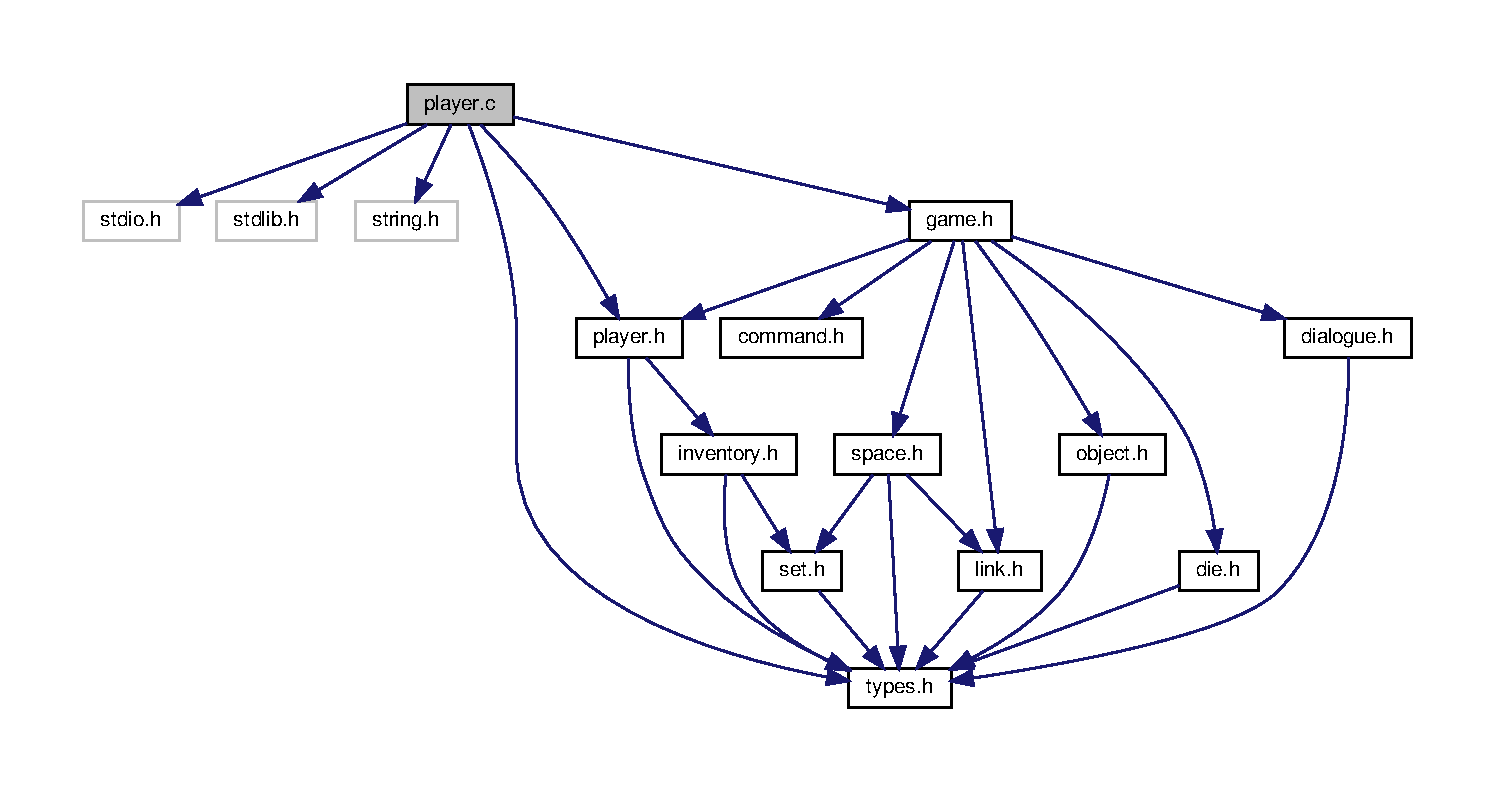
\includegraphics[width=350pt]{player_8c__incl}
\end{center}
\end{figure}
\subsection*{Data Structures}
\begin{DoxyCompactItemize}
\item 
struct \hyperlink{struct__Player}{\+\_\+\+Player}
\begin{DoxyCompactList}\small\item\em defines the structure of player \end{DoxyCompactList}\end{DoxyCompactItemize}
\subsection*{Functions}
\begin{DoxyCompactItemize}
\item 
\hyperlink{player_8h_af30e2030635a69690f85e48bc6ef202f}{Player} $\ast$ \hyperlink{player_8c_a97ea1d0deda3c51ef6ce63a13dab7a38}{player\+\_\+create} (\hyperlink{types_8h_a845e604fb28f7e3d97549da3448149d3}{Id} id)
\begin{DoxyCompactList}\small\item\em create the player in the game \end{DoxyCompactList}\item 
\hyperlink{types_8h_a32c27cc471df37f4fc818d65de0a56c4}{S\+T\+A\+T\+US} \hyperlink{player_8c_a68e324aa5064e27d0a2f38aafb6809ad}{player\+\_\+destroy} (\hyperlink{player_8h_af30e2030635a69690f85e48bc6ef202f}{Player} $\ast$player)
\begin{DoxyCompactList}\small\item\em destroy the player in the game \end{DoxyCompactList}\item 
\hyperlink{types_8h_a32c27cc471df37f4fc818d65de0a56c4}{S\+T\+A\+T\+US} \hyperlink{player_8c_a6a30809f7775f5c2d3bef47d92769e59}{player\+\_\+set\+\_\+name} (\hyperlink{player_8h_af30e2030635a69690f85e48bc6ef202f}{Player} $\ast$player, char $\ast$name)
\begin{DoxyCompactList}\small\item\em set the name of player \end{DoxyCompactList}\item 
\hyperlink{types_8h_a32c27cc471df37f4fc818d65de0a56c4}{S\+T\+A\+T\+US} \hyperlink{player_8c_ac8ace1a1b6b11bc7f92a71a3922e4b83}{player\+\_\+set\+\_\+location} (\hyperlink{player_8h_af30e2030635a69690f85e48bc6ef202f}{Player} $\ast$player, \hyperlink{types_8h_a845e604fb28f7e3d97549da3448149d3}{Id} id)
\begin{DoxyCompactList}\small\item\em set the location of player \end{DoxyCompactList}\item 
\hyperlink{types_8h_a32c27cc471df37f4fc818d65de0a56c4}{S\+T\+A\+T\+US} \hyperlink{player_8c_a7d6f74705bcee19a39dba6e8a04895bd}{player\+\_\+add\+\_\+object} (\hyperlink{player_8h_af30e2030635a69690f85e48bc6ef202f}{Player} $\ast$player, \hyperlink{types_8h_a845e604fb28f7e3d97549da3448149d3}{Id} value)
\begin{DoxyCompactList}\small\item\em add an object to player \end{DoxyCompactList}\item 
\hyperlink{types_8h_a32c27cc471df37f4fc818d65de0a56c4}{S\+T\+A\+T\+US} \hyperlink{player_8c_af2db603fc8e7abdeac681a34461dc21a}{player\+\_\+set\+\_\+object} (\hyperlink{player_8h_af30e2030635a69690f85e48bc6ef202f}{Player} $\ast$player, \hyperlink{types_8h_a845e604fb28f7e3d97549da3448149d3}{Id} value, int pos)
\begin{DoxyCompactList}\small\item\em set an object to player \end{DoxyCompactList}\item 
\hyperlink{types_8h_a32c27cc471df37f4fc818d65de0a56c4}{S\+T\+A\+T\+US} \hyperlink{player_8c_a68871bc282449eb64b977acbdbd7565a}{player\+\_\+del\+\_\+object} (\hyperlink{player_8h_af30e2030635a69690f85e48bc6ef202f}{Player} $\ast$player, \hyperlink{types_8h_a845e604fb28f7e3d97549da3448149d3}{Id} id)
\begin{DoxyCompactList}\small\item\em object to player \end{DoxyCompactList}\item 
const char $\ast$ \hyperlink{player_8c_a6622c02be2fe230a5c0df66385a13ece}{player\+\_\+get\+\_\+name} (\hyperlink{player_8h_af30e2030635a69690f85e48bc6ef202f}{Player} $\ast$player)
\begin{DoxyCompactList}\small\item\em get the name of player \end{DoxyCompactList}\item 
\hyperlink{types_8h_a845e604fb28f7e3d97549da3448149d3}{Id} \hyperlink{player_8c_af5a101ec91427951c5875569a8709956}{player\+\_\+get\+\_\+id} (\hyperlink{player_8h_af30e2030635a69690f85e48bc6ef202f}{Player} $\ast$player)
\begin{DoxyCompactList}\small\item\em get the id of player \end{DoxyCompactList}\item 
\hyperlink{types_8h_a845e604fb28f7e3d97549da3448149d3}{Id} \hyperlink{player_8c_aa50ce77ab79af7166d749619fd60acfe}{player\+\_\+get\+\_\+location} (\hyperlink{player_8h_af30e2030635a69690f85e48bc6ef202f}{Player} $\ast$player)
\begin{DoxyCompactList}\small\item\em get the location of player \end{DoxyCompactList}\item 
\hyperlink{types_8h_a845e604fb28f7e3d97549da3448149d3}{Id} \hyperlink{player_8c_a6d1473d0cb2940463f49253d3a88f462}{player\+\_\+get\+\_\+object} (\hyperlink{player_8h_af30e2030635a69690f85e48bc6ef202f}{Player} $\ast$player, int pos)
\begin{DoxyCompactList}\small\item\em get the object of player \end{DoxyCompactList}\item 
\hyperlink{types_8h_a32c27cc471df37f4fc818d65de0a56c4}{S\+T\+A\+T\+US} \hyperlink{player_8c_aa0f2f8b4d1b63a60ef927d47aa45dbd1}{player\+\_\+print} (\hyperlink{player_8h_af30e2030635a69690f85e48bc6ef202f}{Player} $\ast$player)
\begin{DoxyCompactList}\small\item\em print the player \end{DoxyCompactList}\end{DoxyCompactItemize}


\subsection{Detailed Description}
It defines the header of the module player. 

\begin{DoxyAuthor}{Author}
\end{DoxyAuthor}
\begin{DoxyVersion}{Version}
2.\+0 
\end{DoxyVersion}
\begin{DoxyDate}{Date}
15-\/02-\/2019 
\end{DoxyDate}
\begin{DoxyCopyright}{Copyright}
G\+NU Public License 
\end{DoxyCopyright}


\subsection{Function Documentation}
\mbox{\Hypertarget{player_8c_a7d6f74705bcee19a39dba6e8a04895bd}\label{player_8c_a7d6f74705bcee19a39dba6e8a04895bd}} 
\index{player.\+c@{player.\+c}!player\+\_\+add\+\_\+object@{player\+\_\+add\+\_\+object}}
\index{player\+\_\+add\+\_\+object@{player\+\_\+add\+\_\+object}!player.\+c@{player.\+c}}
\subsubsection{\texorpdfstring{player\+\_\+add\+\_\+object()}{player\_add\_object()}}
{\footnotesize\ttfamily \hyperlink{types_8h_a32c27cc471df37f4fc818d65de0a56c4}{S\+T\+A\+T\+US} player\+\_\+add\+\_\+object (\begin{DoxyParamCaption}\item[{\hyperlink{player_8h_af30e2030635a69690f85e48bc6ef202f}{Player} $\ast$}]{player,  }\item[{\hyperlink{types_8h_a845e604fb28f7e3d97549da3448149d3}{Id}}]{value }\end{DoxyParamCaption})}



add an object to player 


\begin{DoxyParams}{Parameters}
{\em player} & \\
\hline
{\em value} & \\
\hline
\end{DoxyParams}
\begin{DoxyReturn}{Returns}
OK, or E\+R\+R\+OR 
\end{DoxyReturn}
\mbox{\Hypertarget{player_8c_a97ea1d0deda3c51ef6ce63a13dab7a38}\label{player_8c_a97ea1d0deda3c51ef6ce63a13dab7a38}} 
\index{player.\+c@{player.\+c}!player\+\_\+create@{player\+\_\+create}}
\index{player\+\_\+create@{player\+\_\+create}!player.\+c@{player.\+c}}
\subsubsection{\texorpdfstring{player\+\_\+create()}{player\_create()}}
{\footnotesize\ttfamily \hyperlink{player_8h_af30e2030635a69690f85e48bc6ef202f}{Player}$\ast$ player\+\_\+create (\begin{DoxyParamCaption}\item[{\hyperlink{types_8h_a845e604fb28f7e3d97549da3448149d3}{Id}}]{id }\end{DoxyParamCaption})}



create the player in the game 


\begin{DoxyParams}{Parameters}
{\em id} & \\
\hline
\end{DoxyParams}
\begin{DoxyReturn}{Returns}
player or in case of error N\+U\+LL 
\end{DoxyReturn}
\mbox{\Hypertarget{player_8c_a68871bc282449eb64b977acbdbd7565a}\label{player_8c_a68871bc282449eb64b977acbdbd7565a}} 
\index{player.\+c@{player.\+c}!player\+\_\+del\+\_\+object@{player\+\_\+del\+\_\+object}}
\index{player\+\_\+del\+\_\+object@{player\+\_\+del\+\_\+object}!player.\+c@{player.\+c}}
\subsubsection{\texorpdfstring{player\+\_\+del\+\_\+object()}{player\_del\_object()}}
{\footnotesize\ttfamily \hyperlink{types_8h_a32c27cc471df37f4fc818d65de0a56c4}{S\+T\+A\+T\+US} player\+\_\+del\+\_\+object (\begin{DoxyParamCaption}\item[{\hyperlink{player_8h_af30e2030635a69690f85e48bc6ef202f}{Player} $\ast$}]{player,  }\item[{\hyperlink{types_8h_a845e604fb28f7e3d97549da3448149d3}{Id}}]{id }\end{DoxyParamCaption})}



object to player 


\begin{DoxyParams}{Parameters}
{\em player} & \\
\hline
{\em id} & \\
\hline
\end{DoxyParams}
\begin{DoxyReturn}{Returns}
OK, or E\+R\+R\+OR 
\end{DoxyReturn}
\mbox{\Hypertarget{player_8c_a68e324aa5064e27d0a2f38aafb6809ad}\label{player_8c_a68e324aa5064e27d0a2f38aafb6809ad}} 
\index{player.\+c@{player.\+c}!player\+\_\+destroy@{player\+\_\+destroy}}
\index{player\+\_\+destroy@{player\+\_\+destroy}!player.\+c@{player.\+c}}
\subsubsection{\texorpdfstring{player\+\_\+destroy()}{player\_destroy()}}
{\footnotesize\ttfamily \hyperlink{types_8h_a32c27cc471df37f4fc818d65de0a56c4}{S\+T\+A\+T\+US} player\+\_\+destroy (\begin{DoxyParamCaption}\item[{\hyperlink{player_8h_af30e2030635a69690f85e48bc6ef202f}{Player} $\ast$}]{player }\end{DoxyParamCaption})}



destroy the player in the game 


\begin{DoxyParams}{Parameters}
{\em player} & \\
\hline
\end{DoxyParams}
\begin{DoxyReturn}{Returns}
OK, or E\+R\+R\+OR 
\end{DoxyReturn}
\mbox{\Hypertarget{player_8c_af5a101ec91427951c5875569a8709956}\label{player_8c_af5a101ec91427951c5875569a8709956}} 
\index{player.\+c@{player.\+c}!player\+\_\+get\+\_\+id@{player\+\_\+get\+\_\+id}}
\index{player\+\_\+get\+\_\+id@{player\+\_\+get\+\_\+id}!player.\+c@{player.\+c}}
\subsubsection{\texorpdfstring{player\+\_\+get\+\_\+id()}{player\_get\_id()}}
{\footnotesize\ttfamily \hyperlink{types_8h_a845e604fb28f7e3d97549da3448149d3}{Id} player\+\_\+get\+\_\+id (\begin{DoxyParamCaption}\item[{\hyperlink{player_8h_af30e2030635a69690f85e48bc6ef202f}{Player} $\ast$}]{player }\end{DoxyParamCaption})}



get the id of player 


\begin{DoxyParams}{Parameters}
{\em player} & \\
\hline
\end{DoxyParams}
\begin{DoxyReturn}{Returns}
id or in case of error N\+U\+LL 
\end{DoxyReturn}
\mbox{\Hypertarget{player_8c_aa50ce77ab79af7166d749619fd60acfe}\label{player_8c_aa50ce77ab79af7166d749619fd60acfe}} 
\index{player.\+c@{player.\+c}!player\+\_\+get\+\_\+location@{player\+\_\+get\+\_\+location}}
\index{player\+\_\+get\+\_\+location@{player\+\_\+get\+\_\+location}!player.\+c@{player.\+c}}
\subsubsection{\texorpdfstring{player\+\_\+get\+\_\+location()}{player\_get\_location()}}
{\footnotesize\ttfamily \hyperlink{types_8h_a845e604fb28f7e3d97549da3448149d3}{Id} player\+\_\+get\+\_\+location (\begin{DoxyParamCaption}\item[{\hyperlink{player_8h_af30e2030635a69690f85e48bc6ef202f}{Player} $\ast$}]{player }\end{DoxyParamCaption})}



get the location of player 


\begin{DoxyParams}{Parameters}
{\em player} & \\
\hline
\end{DoxyParams}
\begin{DoxyReturn}{Returns}
id or in case of error N\+U\+LL 
\end{DoxyReturn}
\mbox{\Hypertarget{player_8c_a6622c02be2fe230a5c0df66385a13ece}\label{player_8c_a6622c02be2fe230a5c0df66385a13ece}} 
\index{player.\+c@{player.\+c}!player\+\_\+get\+\_\+name@{player\+\_\+get\+\_\+name}}
\index{player\+\_\+get\+\_\+name@{player\+\_\+get\+\_\+name}!player.\+c@{player.\+c}}
\subsubsection{\texorpdfstring{player\+\_\+get\+\_\+name()}{player\_get\_name()}}
{\footnotesize\ttfamily const char$\ast$ player\+\_\+get\+\_\+name (\begin{DoxyParamCaption}\item[{\hyperlink{player_8h_af30e2030635a69690f85e48bc6ef202f}{Player} $\ast$}]{player }\end{DoxyParamCaption})}



get the name of player 


\begin{DoxyParams}{Parameters}
{\em player} & \\
\hline
\end{DoxyParams}
\begin{DoxyReturn}{Returns}
name of player or in case of error N\+U\+LL 
\end{DoxyReturn}
\mbox{\Hypertarget{player_8c_a6d1473d0cb2940463f49253d3a88f462}\label{player_8c_a6d1473d0cb2940463f49253d3a88f462}} 
\index{player.\+c@{player.\+c}!player\+\_\+get\+\_\+object@{player\+\_\+get\+\_\+object}}
\index{player\+\_\+get\+\_\+object@{player\+\_\+get\+\_\+object}!player.\+c@{player.\+c}}
\subsubsection{\texorpdfstring{player\+\_\+get\+\_\+object()}{player\_get\_object()}}
{\footnotesize\ttfamily \hyperlink{types_8h_a845e604fb28f7e3d97549da3448149d3}{Id} player\+\_\+get\+\_\+object (\begin{DoxyParamCaption}\item[{\hyperlink{player_8h_af30e2030635a69690f85e48bc6ef202f}{Player} $\ast$}]{player,  }\item[{int}]{pos }\end{DoxyParamCaption})}



get the object of player 


\begin{DoxyParams}{Parameters}
{\em player} & \\
\hline
{\em pos} & \\
\hline
\end{DoxyParams}
\begin{DoxyReturn}{Returns}
id or in case of error N\+U\+LL 
\end{DoxyReturn}
\mbox{\Hypertarget{player_8c_aa0f2f8b4d1b63a60ef927d47aa45dbd1}\label{player_8c_aa0f2f8b4d1b63a60ef927d47aa45dbd1}} 
\index{player.\+c@{player.\+c}!player\+\_\+print@{player\+\_\+print}}
\index{player\+\_\+print@{player\+\_\+print}!player.\+c@{player.\+c}}
\subsubsection{\texorpdfstring{player\+\_\+print()}{player\_print()}}
{\footnotesize\ttfamily \hyperlink{types_8h_a32c27cc471df37f4fc818d65de0a56c4}{S\+T\+A\+T\+US} player\+\_\+print (\begin{DoxyParamCaption}\item[{\hyperlink{player_8h_af30e2030635a69690f85e48bc6ef202f}{Player} $\ast$}]{player }\end{DoxyParamCaption})}



print the player 


\begin{DoxyParams}{Parameters}
{\em player} & \\
\hline
\end{DoxyParams}
\begin{DoxyReturn}{Returns}
OK, or E\+R\+R\+OR 
\end{DoxyReturn}
\mbox{\Hypertarget{player_8c_ac8ace1a1b6b11bc7f92a71a3922e4b83}\label{player_8c_ac8ace1a1b6b11bc7f92a71a3922e4b83}} 
\index{player.\+c@{player.\+c}!player\+\_\+set\+\_\+location@{player\+\_\+set\+\_\+location}}
\index{player\+\_\+set\+\_\+location@{player\+\_\+set\+\_\+location}!player.\+c@{player.\+c}}
\subsubsection{\texorpdfstring{player\+\_\+set\+\_\+location()}{player\_set\_location()}}
{\footnotesize\ttfamily \hyperlink{types_8h_a32c27cc471df37f4fc818d65de0a56c4}{S\+T\+A\+T\+US} player\+\_\+set\+\_\+location (\begin{DoxyParamCaption}\item[{\hyperlink{player_8h_af30e2030635a69690f85e48bc6ef202f}{Player} $\ast$}]{player,  }\item[{\hyperlink{types_8h_a845e604fb28f7e3d97549da3448149d3}{Id}}]{id }\end{DoxyParamCaption})}



set the location of player 


\begin{DoxyParams}{Parameters}
{\em player} & \\
\hline
{\em id} & \\
\hline
\end{DoxyParams}
\begin{DoxyReturn}{Returns}
OK, or E\+R\+R\+OR 
\end{DoxyReturn}
\mbox{\Hypertarget{player_8c_a6a30809f7775f5c2d3bef47d92769e59}\label{player_8c_a6a30809f7775f5c2d3bef47d92769e59}} 
\index{player.\+c@{player.\+c}!player\+\_\+set\+\_\+name@{player\+\_\+set\+\_\+name}}
\index{player\+\_\+set\+\_\+name@{player\+\_\+set\+\_\+name}!player.\+c@{player.\+c}}
\subsubsection{\texorpdfstring{player\+\_\+set\+\_\+name()}{player\_set\_name()}}
{\footnotesize\ttfamily \hyperlink{types_8h_a32c27cc471df37f4fc818d65de0a56c4}{S\+T\+A\+T\+US} player\+\_\+set\+\_\+name (\begin{DoxyParamCaption}\item[{\hyperlink{player_8h_af30e2030635a69690f85e48bc6ef202f}{Player} $\ast$}]{player,  }\item[{char $\ast$}]{name }\end{DoxyParamCaption})}



set the name of player 


\begin{DoxyParams}{Parameters}
{\em player} & \\
\hline
{\em name} & \\
\hline
\end{DoxyParams}
\begin{DoxyReturn}{Returns}
OK, or E\+R\+R\+OR 
\end{DoxyReturn}
\mbox{\Hypertarget{player_8c_af2db603fc8e7abdeac681a34461dc21a}\label{player_8c_af2db603fc8e7abdeac681a34461dc21a}} 
\index{player.\+c@{player.\+c}!player\+\_\+set\+\_\+object@{player\+\_\+set\+\_\+object}}
\index{player\+\_\+set\+\_\+object@{player\+\_\+set\+\_\+object}!player.\+c@{player.\+c}}
\subsubsection{\texorpdfstring{player\+\_\+set\+\_\+object()}{player\_set\_object()}}
{\footnotesize\ttfamily \hyperlink{types_8h_a32c27cc471df37f4fc818d65de0a56c4}{S\+T\+A\+T\+US} player\+\_\+set\+\_\+object (\begin{DoxyParamCaption}\item[{\hyperlink{player_8h_af30e2030635a69690f85e48bc6ef202f}{Player} $\ast$}]{player,  }\item[{\hyperlink{types_8h_a845e604fb28f7e3d97549da3448149d3}{Id}}]{value,  }\item[{int}]{pos }\end{DoxyParamCaption})}



set an object to player 


\begin{DoxyParams}{Parameters}
{\em player} & \\
\hline
{\em value} & \\
\hline
{\em pos} & \\
\hline
\end{DoxyParams}
\begin{DoxyReturn}{Returns}
OK, or E\+R\+R\+OR 
\end{DoxyReturn}


\hypertarget{player_8h}{\section{include/player.h File Reference}
\label{player_8h}\index{include/player.\+h@{include/player.\+h}}
}


It defines a player.  


{\ttfamily \#include \char`\"{}../include/types.\+h\char`\"{}}\\*
{\ttfamily \#include \char`\"{}../include/set.\+h\char`\"{}}\\*
{\ttfamily \#include \char`\"{}../include/inventory.\+h\char`\"{}}\\*
Include dependency graph for player.\+h\+:
\nopagebreak
\begin{figure}[H]
\begin{center}
\leavevmode
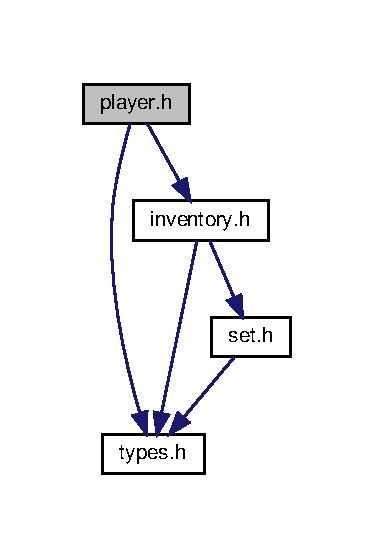
\includegraphics[width=344pt]{player_8h__incl}
\end{center}
\end{figure}
This graph shows which files directly or indirectly include this file\+:
\nopagebreak
\begin{figure}[H]
\begin{center}
\leavevmode
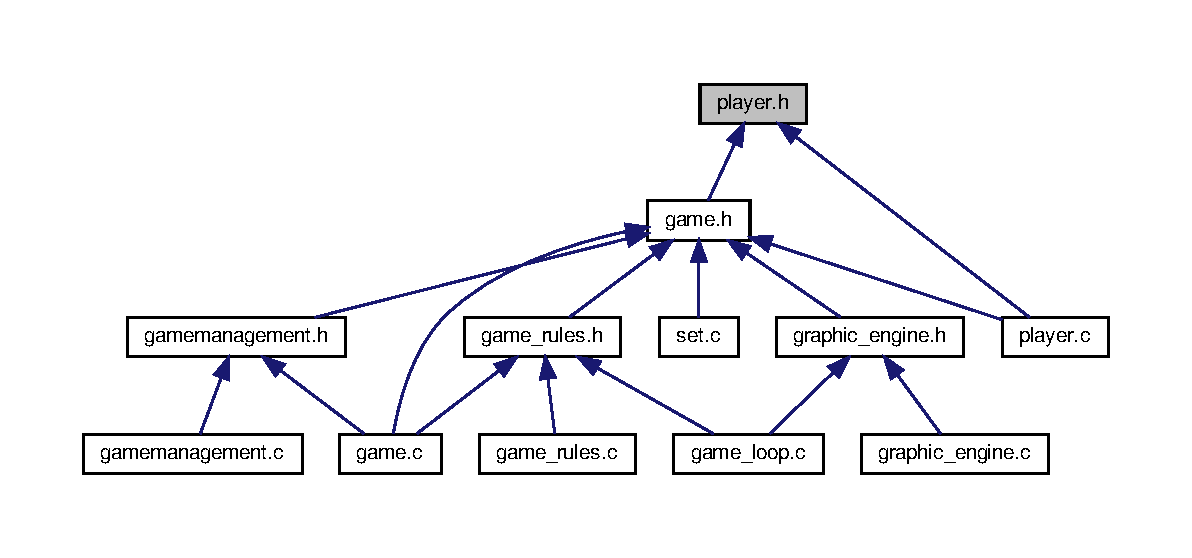
\includegraphics[width=350pt]{player_8h__dep__incl}
\end{center}
\end{figure}
\subsection*{Typedefs}
\begin{DoxyCompactItemize}
\item 
\hypertarget{player_8h_af30e2030635a69690f85e48bc6ef202f}{typedef struct \hyperlink{struct__Player}{\+\_\+\+Player} \hyperlink{player_8h_af30e2030635a69690f85e48bc6ef202f}{Player}}\label{player_8h_af30e2030635a69690f85e48bc6ef202f}

\begin{DoxyCompactList}\small\item\em Estructura del jugador. \end{DoxyCompactList}\end{DoxyCompactItemize}
\subsection*{Functions}
\begin{DoxyCompactItemize}
\item 
\hyperlink{player_8h_af30e2030635a69690f85e48bc6ef202f}{Player} $\ast$ \hyperlink{player_8h_a97ea1d0deda3c51ef6ce63a13dab7a38}{player\+\_\+create} (\hyperlink{types_8h_a845e604fb28f7e3d97549da3448149d3}{Id} id)
\begin{DoxyCompactList}\small\item\em Funcion para inicializar el jugador Funcion encargada de reservar espacio para el jugador e inizializar sus parametros. \end{DoxyCompactList}\item 
\hyperlink{types_8h_a32c27cc471df37f4fc818d65de0a56c4}{S\+T\+A\+T\+U\+S} \hyperlink{player_8h_a68e324aa5064e27d0a2f38aafb6809ad}{player\+\_\+destroy} (\hyperlink{player_8h_af30e2030635a69690f85e48bc6ef202f}{Player} $\ast$player)
\begin{DoxyCompactList}\small\item\em Funcion encargada de liberar la memoria reservada para el jugador. \end{DoxyCompactList}\item 
\hyperlink{types_8h_a32c27cc471df37f4fc818d65de0a56c4}{S\+T\+A\+T\+U\+S} \hyperlink{player_8h_a6a30809f7775f5c2d3bef47d92769e59}{player\+\_\+set\+\_\+name} (\hyperlink{player_8h_af30e2030635a69690f85e48bc6ef202f}{Player} $\ast$player, char $\ast$name)
\begin{DoxyCompactList}\small\item\em Funcion encargada de cambiar el nombre del. \end{DoxyCompactList}\item 
\hyperlink{types_8h_a32c27cc471df37f4fc818d65de0a56c4}{S\+T\+A\+T\+U\+S} \hyperlink{player_8h_af92901f53a33ee9083a14fd947898e06}{player\+\_\+set\+\_\+space} (\hyperlink{player_8h_af30e2030635a69690f85e48bc6ef202f}{Player} $\ast$player, \hyperlink{types_8h_a845e604fb28f7e3d97549da3448149d3}{Id} id)
\begin{DoxyCompactList}\small\item\em Funcion encargada de cambiar el espacio en el que se encuentra. \end{DoxyCompactList}\item 
\hyperlink{types_8h_a32c27cc471df37f4fc818d65de0a56c4}{S\+T\+A\+T\+U\+S} \hyperlink{player_8h_af5eacaf6a51631f28500d8127e761c1b}{player\+\_\+set\+\_\+object} (\hyperlink{player_8h_af30e2030635a69690f85e48bc6ef202f}{Player} $\ast$player, \hyperlink{types_8h_a845e604fb28f7e3d97549da3448149d3}{Id} id)
\begin{DoxyCompactList}\small\item\em Funcion encargada de añadir un objeto al jugador. \end{DoxyCompactList}\item 
\hyperlink{types_8h_a32c27cc471df37f4fc818d65de0a56c4}{S\+T\+A\+T\+U\+S} \hyperlink{player_8h_a523d1c79f53c3ce0da06bd186520d35d}{player\+\_\+set\+\_\+inventory} (\hyperlink{player_8h_af30e2030635a69690f85e48bc6ef202f}{Player} $\ast$player, \hyperlink{inventory_8h_a2253bf64ac4ce6a9c1d6f39c0b0d32a3}{Inventory} $\ast$inventorio)
\begin{DoxyCompactList}\small\item\em Funcion encargada de asignarle un inventorio al jugador Funcion usada para cargar los inventorios desde un archivo. \end{DoxyCompactList}\item 
const char $\ast$ \hyperlink{player_8h_a6622c02be2fe230a5c0df66385a13ece}{player\+\_\+get\+\_\+name} (\hyperlink{player_8h_af30e2030635a69690f85e48bc6ef202f}{Player} $\ast$player)
\begin{DoxyCompactList}\small\item\em Funcion encargada de obtener el nombre del jugador. \end{DoxyCompactList}\item 
\hyperlink{types_8h_a845e604fb28f7e3d97549da3448149d3}{Id} \hyperlink{player_8h_af5a101ec91427951c5875569a8709956}{player\+\_\+get\+\_\+id} (\hyperlink{player_8h_af30e2030635a69690f85e48bc6ef202f}{Player} $\ast$player)
\begin{DoxyCompactList}\small\item\em Funcion encargada de obtener el id del jugador. \end{DoxyCompactList}\item 
\hyperlink{types_8h_a845e604fb28f7e3d97549da3448149d3}{Id} \hyperlink{player_8h_a4eabc7f4e8d852ef582ee331c104207c}{player\+\_\+get\+\_\+space} (\hyperlink{player_8h_af30e2030635a69690f85e48bc6ef202f}{Player} $\ast$player)
\begin{DoxyCompactList}\small\item\em Funcion encargada de obtener el id del espacio donde se encuentra el jugador. \end{DoxyCompactList}\item 
\hyperlink{types_8h_a3e5b8192e7d9ffaf3542f1210aec18dd}{B\+O\+O\+L} \hyperlink{player_8h_a8deed220c7807d597a8765e3d131d1d9}{player\+\_\+get\+\_\+object} (\hyperlink{player_8h_af30e2030635a69690f85e48bc6ef202f}{Player} $\ast$player, \hyperlink{types_8h_a845e604fb28f7e3d97549da3448149d3}{Id} id)
\begin{DoxyCompactList}\small\item\em Funcion encargada de ver si el jugador tiene un objeto. \end{DoxyCompactList}\item 
\hyperlink{set_8h_a6d3b7f7c92cbb4577ef3ef7ddbf93161}{Set} $\ast$ \hyperlink{player_8h_ac2abf0830926be3f9cfacd09cc8a4f39}{player\+\_\+get\+\_\+objects} (\hyperlink{player_8h_af30e2030635a69690f85e48bc6ef202f}{Player} $\ast$player)
\begin{DoxyCompactList}\small\item\em Funcion encargada de devolver los ids de los objetos del jugador. \end{DoxyCompactList}\item 
\hyperlink{inventory_8h_a2253bf64ac4ce6a9c1d6f39c0b0d32a3}{Inventory} $\ast$ \hyperlink{player_8h_a270da6469a85e0c2b7f9f4088d290051}{player\+\_\+get\+\_\+inventory} (\hyperlink{player_8h_af30e2030635a69690f85e48bc6ef202f}{Player} $\ast$player)
\begin{DoxyCompactList}\small\item\em Funcion para obtener el inventorio del jugador Esta función se usa para guardar en el fichero los datos del juego actual. \end{DoxyCompactList}\item 
size\+\_\+t \hyperlink{player_8h_a0db3f153d7d3635b0163400a48afa4c4}{player\+\_\+get\+\_\+size} ()
\begin{DoxyCompactList}\small\item\em Funcion encargada de devolver el tamaño del jugador. \end{DoxyCompactList}\item 
\hyperlink{types_8h_a32c27cc471df37f4fc818d65de0a56c4}{S\+T\+A\+T\+U\+S} \hyperlink{player_8h_a0306b5f6a99481b01994c11500fe5901}{player\+\_\+del\+\_\+objects} (\hyperlink{player_8h_af30e2030635a69690f85e48bc6ef202f}{Player} $\ast$player, \hyperlink{types_8h_a845e604fb28f7e3d97549da3448149d3}{Id} id)
\begin{DoxyCompactList}\small\item\em Funcion encargada de borrar objetos del set del jugador. \end{DoxyCompactList}\item 
\hyperlink{types_8h_a32c27cc471df37f4fc818d65de0a56c4}{S\+T\+A\+T\+U\+S} \hyperlink{player_8h_aa0f2f8b4d1b63a60ef927d47aa45dbd1}{player\+\_\+print} (\hyperlink{player_8h_af30e2030635a69690f85e48bc6ef202f}{Player} $\ast$player)
\begin{DoxyCompactList}\small\item\em Funcion para imprimir los datos del jugador. \end{DoxyCompactList}\end{DoxyCompactItemize}


\subsection{Detailed Description}
It defines a player. 

\begin{DoxyAuthor}{Author}
Cristina Soria 
\end{DoxyAuthor}
\begin{DoxyVersion}{Version}
2.\+0 
\end{DoxyVersion}
\begin{DoxyDate}{Date}
22/03/2018 
\end{DoxyDate}


\subsection{Function Documentation}
\hypertarget{player_8h_a97ea1d0deda3c51ef6ce63a13dab7a38}{\index{player.\+h@{player.\+h}!player\+\_\+create@{player\+\_\+create}}
\index{player\+\_\+create@{player\+\_\+create}!player.\+h@{player.\+h}}
\subsubsection[{player\+\_\+create}]{\setlength{\rightskip}{0pt plus 5cm}{\bf Player}$\ast$ player\+\_\+create (
\begin{DoxyParamCaption}
\item[{{\bf Id}}]{id}
\end{DoxyParamCaption}
)}}\label{player_8h_a97ea1d0deda3c51ef6ce63a13dab7a38}


Funcion para inicializar el jugador Funcion encargada de reservar espacio para el jugador e inizializar sus parametros. 

\begin{DoxyAuthor}{Author}
Miguel Rodriguez 
\end{DoxyAuthor}

\begin{DoxyParams}{Parameters}
{\em id} & se corresponde con el id del jugador \\
\hline
\end{DoxyParams}
\begin{DoxyReturn}{Returns}
El jugador creado 
\end{DoxyReturn}
\hypertarget{player_8h_a0306b5f6a99481b01994c11500fe5901}{\index{player.\+h@{player.\+h}!player\+\_\+del\+\_\+objects@{player\+\_\+del\+\_\+objects}}
\index{player\+\_\+del\+\_\+objects@{player\+\_\+del\+\_\+objects}!player.\+h@{player.\+h}}
\subsubsection[{player\+\_\+del\+\_\+objects}]{\setlength{\rightskip}{0pt plus 5cm}{\bf S\+T\+A\+T\+U\+S} player\+\_\+del\+\_\+objects (
\begin{DoxyParamCaption}
\item[{{\bf Player} $\ast$}]{player, }
\item[{{\bf Id}}]{id}
\end{DoxyParamCaption}
)}}\label{player_8h_a0306b5f6a99481b01994c11500fe5901}


Funcion encargada de borrar objetos del set del jugador. 

\begin{DoxyAuthor}{Author}
Julia Simon 
\end{DoxyAuthor}

\begin{DoxyParams}{Parameters}
{\em player} & jugador \\
\hline
{\em id} & id que quiero eliminar del set \\
\hline
\end{DoxyParams}
\begin{DoxyReturn}{Returns}
O\+K funcionamiento correcto, E\+R\+R\+O\+R caso contrario 
\end{DoxyReturn}
\hypertarget{player_8h_a68e324aa5064e27d0a2f38aafb6809ad}{\index{player.\+h@{player.\+h}!player\+\_\+destroy@{player\+\_\+destroy}}
\index{player\+\_\+destroy@{player\+\_\+destroy}!player.\+h@{player.\+h}}
\subsubsection[{player\+\_\+destroy}]{\setlength{\rightskip}{0pt plus 5cm}{\bf S\+T\+A\+T\+U\+S} player\+\_\+destroy (
\begin{DoxyParamCaption}
\item[{{\bf Player} $\ast$}]{player}
\end{DoxyParamCaption}
)}}\label{player_8h_a68e324aa5064e27d0a2f38aafb6809ad}


Funcion encargada de liberar la memoria reservada para el jugador. 

\begin{DoxyAuthor}{Author}
Miguel Rodriguez 
\end{DoxyAuthor}

\begin{DoxyParams}{Parameters}
{\em player} & jugador a destruir \\
\hline
\end{DoxyParams}
\begin{DoxyReturn}{Returns}
si se ha hecho o no correctamente 
\end{DoxyReturn}
\hypertarget{player_8h_af5a101ec91427951c5875569a8709956}{\index{player.\+h@{player.\+h}!player\+\_\+get\+\_\+id@{player\+\_\+get\+\_\+id}}
\index{player\+\_\+get\+\_\+id@{player\+\_\+get\+\_\+id}!player.\+h@{player.\+h}}
\subsubsection[{player\+\_\+get\+\_\+id}]{\setlength{\rightskip}{0pt plus 5cm}{\bf Id} player\+\_\+get\+\_\+id (
\begin{DoxyParamCaption}
\item[{{\bf Player} $\ast$}]{player}
\end{DoxyParamCaption}
)}}\label{player_8h_af5a101ec91427951c5875569a8709956}


Funcion encargada de obtener el id del jugador. 

\begin{DoxyAuthor}{Author}
Miguel Rodriguez 
\end{DoxyAuthor}

\begin{DoxyParams}{Parameters}
{\em player} & jugador \\
\hline
\end{DoxyParams}
\begin{DoxyReturn}{Returns}
nombre del jugador 
\end{DoxyReturn}
\hypertarget{player_8h_a270da6469a85e0c2b7f9f4088d290051}{\index{player.\+h@{player.\+h}!player\+\_\+get\+\_\+inventory@{player\+\_\+get\+\_\+inventory}}
\index{player\+\_\+get\+\_\+inventory@{player\+\_\+get\+\_\+inventory}!player.\+h@{player.\+h}}
\subsubsection[{player\+\_\+get\+\_\+inventory}]{\setlength{\rightskip}{0pt plus 5cm}{\bf Inventory}$\ast$ player\+\_\+get\+\_\+inventory (
\begin{DoxyParamCaption}
\item[{{\bf Player} $\ast$}]{player}
\end{DoxyParamCaption}
)}}\label{player_8h_a270da6469a85e0c2b7f9f4088d290051}


Funcion para obtener el inventorio del jugador Esta función se usa para guardar en el fichero los datos del juego actual. 

\begin{DoxyAuthor}{Author}
Julia Simon 
\end{DoxyAuthor}

\begin{DoxyParams}{Parameters}
{\em player} & jugador \\
\hline
\end{DoxyParams}
\begin{DoxyReturn}{Returns}
verdadero si tiene objeto, falso caso contrario 
\end{DoxyReturn}
\hypertarget{player_8h_a6622c02be2fe230a5c0df66385a13ece}{\index{player.\+h@{player.\+h}!player\+\_\+get\+\_\+name@{player\+\_\+get\+\_\+name}}
\index{player\+\_\+get\+\_\+name@{player\+\_\+get\+\_\+name}!player.\+h@{player.\+h}}
\subsubsection[{player\+\_\+get\+\_\+name}]{\setlength{\rightskip}{0pt plus 5cm}const char$\ast$ player\+\_\+get\+\_\+name (
\begin{DoxyParamCaption}
\item[{{\bf Player} $\ast$}]{player}
\end{DoxyParamCaption}
)}}\label{player_8h_a6622c02be2fe230a5c0df66385a13ece}


Funcion encargada de obtener el nombre del jugador. 

\begin{DoxyAuthor}{Author}
Miguel Rodriguez 
\end{DoxyAuthor}

\begin{DoxyParams}{Parameters}
{\em player} & jugador \\
\hline
\end{DoxyParams}
\begin{DoxyReturn}{Returns}
nombre del jugador 
\end{DoxyReturn}
\hypertarget{player_8h_a8deed220c7807d597a8765e3d131d1d9}{\index{player.\+h@{player.\+h}!player\+\_\+get\+\_\+object@{player\+\_\+get\+\_\+object}}
\index{player\+\_\+get\+\_\+object@{player\+\_\+get\+\_\+object}!player.\+h@{player.\+h}}
\subsubsection[{player\+\_\+get\+\_\+object}]{\setlength{\rightskip}{0pt plus 5cm}{\bf B\+O\+O\+L} player\+\_\+get\+\_\+object (
\begin{DoxyParamCaption}
\item[{{\bf Player} $\ast$}]{player, }
\item[{{\bf Id}}]{id}
\end{DoxyParamCaption}
)}}\label{player_8h_a8deed220c7807d597a8765e3d131d1d9}


Funcion encargada de ver si el jugador tiene un objeto. 

\begin{DoxyAuthor}{Author}
Julia Simon 
\end{DoxyAuthor}

\begin{DoxyParams}{Parameters}
{\em player} & jugador \\
\hline
\end{DoxyParams}
\begin{DoxyReturn}{Returns}
verdadero si tiene objeto, falso caso contrario 
\end{DoxyReturn}
\hypertarget{player_8h_ac2abf0830926be3f9cfacd09cc8a4f39}{\index{player.\+h@{player.\+h}!player\+\_\+get\+\_\+objects@{player\+\_\+get\+\_\+objects}}
\index{player\+\_\+get\+\_\+objects@{player\+\_\+get\+\_\+objects}!player.\+h@{player.\+h}}
\subsubsection[{player\+\_\+get\+\_\+objects}]{\setlength{\rightskip}{0pt plus 5cm}{\bf Set}$\ast$ player\+\_\+get\+\_\+objects (
\begin{DoxyParamCaption}
\item[{{\bf Player} $\ast$}]{player}
\end{DoxyParamCaption}
)}}\label{player_8h_ac2abf0830926be3f9cfacd09cc8a4f39}


Funcion encargada de devolver los ids de los objetos del jugador. 

\begin{DoxyAuthor}{Author}
Julia Simon 
\end{DoxyAuthor}

\begin{DoxyParams}{Parameters}
{\em player} & jugador \\
\hline
\end{DoxyParams}
\begin{DoxyReturn}{Returns}
verdadero si tiene objeto, falso caso contrario 
\end{DoxyReturn}
\hypertarget{player_8h_a0db3f153d7d3635b0163400a48afa4c4}{\index{player.\+h@{player.\+h}!player\+\_\+get\+\_\+size@{player\+\_\+get\+\_\+size}}
\index{player\+\_\+get\+\_\+size@{player\+\_\+get\+\_\+size}!player.\+h@{player.\+h}}
\subsubsection[{player\+\_\+get\+\_\+size}]{\setlength{\rightskip}{0pt plus 5cm}size\+\_\+t player\+\_\+get\+\_\+size (
\begin{DoxyParamCaption}
{}
\end{DoxyParamCaption}
)}}\label{player_8h_a0db3f153d7d3635b0163400a48afa4c4}


Funcion encargada de devolver el tamaño del jugador. 

\begin{DoxyAuthor}{Author}
Julia Simon 
\end{DoxyAuthor}
\begin{DoxyReturn}{Returns}
tamaño 
\end{DoxyReturn}
\hypertarget{player_8h_a4eabc7f4e8d852ef582ee331c104207c}{\index{player.\+h@{player.\+h}!player\+\_\+get\+\_\+space@{player\+\_\+get\+\_\+space}}
\index{player\+\_\+get\+\_\+space@{player\+\_\+get\+\_\+space}!player.\+h@{player.\+h}}
\subsubsection[{player\+\_\+get\+\_\+space}]{\setlength{\rightskip}{0pt plus 5cm}{\bf Id} player\+\_\+get\+\_\+space (
\begin{DoxyParamCaption}
\item[{{\bf Player} $\ast$}]{player}
\end{DoxyParamCaption}
)}}\label{player_8h_a4eabc7f4e8d852ef582ee331c104207c}


Funcion encargada de obtener el id del espacio donde se encuentra el jugador. 

\begin{DoxyAuthor}{Author}
Miguel Rodriguez 
\end{DoxyAuthor}

\begin{DoxyParams}{Parameters}
{\em player} & jugador \\
\hline
\end{DoxyParams}
\begin{DoxyReturn}{Returns}
id del espacio 
\end{DoxyReturn}
\hypertarget{player_8h_aa0f2f8b4d1b63a60ef927d47aa45dbd1}{\index{player.\+h@{player.\+h}!player\+\_\+print@{player\+\_\+print}}
\index{player\+\_\+print@{player\+\_\+print}!player.\+h@{player.\+h}}
\subsubsection[{player\+\_\+print}]{\setlength{\rightskip}{0pt plus 5cm}{\bf S\+T\+A\+T\+U\+S} player\+\_\+print (
\begin{DoxyParamCaption}
\item[{{\bf Player} $\ast$}]{player}
\end{DoxyParamCaption}
)}}\label{player_8h_aa0f2f8b4d1b63a60ef927d47aa45dbd1}


Funcion para imprimir los datos del jugador. 

\begin{DoxyAuthor}{Author}
Miguel Rodriguez 
\end{DoxyAuthor}

\begin{DoxyParams}{Parameters}
{\em player} & jugador \\
\hline
\end{DoxyParams}
\begin{DoxyReturn}{Returns}
si se ha hecho o no correctamente 
\end{DoxyReturn}
\hypertarget{player_8h_a523d1c79f53c3ce0da06bd186520d35d}{\index{player.\+h@{player.\+h}!player\+\_\+set\+\_\+inventory@{player\+\_\+set\+\_\+inventory}}
\index{player\+\_\+set\+\_\+inventory@{player\+\_\+set\+\_\+inventory}!player.\+h@{player.\+h}}
\subsubsection[{player\+\_\+set\+\_\+inventory}]{\setlength{\rightskip}{0pt plus 5cm}{\bf S\+T\+A\+T\+U\+S} player\+\_\+set\+\_\+inventory (
\begin{DoxyParamCaption}
\item[{{\bf Player} $\ast$}]{player, }
\item[{{\bf Inventory} $\ast$}]{inventorio}
\end{DoxyParamCaption}
)}}\label{player_8h_a523d1c79f53c3ce0da06bd186520d35d}


Funcion encargada de asignarle un inventorio al jugador Funcion usada para cargar los inventorios desde un archivo. 

\begin{DoxyAuthor}{Author}
Julia Simon 
\end{DoxyAuthor}

\begin{DoxyParams}{Parameters}
{\em player} & jugador \\
\hline
{\em inventorio} & inventorio a añadir \\
\hline
\end{DoxyParams}
\begin{DoxyReturn}{Returns}
si se ha hecho o no correctamente 
\end{DoxyReturn}
\hypertarget{player_8h_a6a30809f7775f5c2d3bef47d92769e59}{\index{player.\+h@{player.\+h}!player\+\_\+set\+\_\+name@{player\+\_\+set\+\_\+name}}
\index{player\+\_\+set\+\_\+name@{player\+\_\+set\+\_\+name}!player.\+h@{player.\+h}}
\subsubsection[{player\+\_\+set\+\_\+name}]{\setlength{\rightskip}{0pt plus 5cm}{\bf S\+T\+A\+T\+U\+S} player\+\_\+set\+\_\+name (
\begin{DoxyParamCaption}
\item[{{\bf Player} $\ast$}]{player, }
\item[{char $\ast$}]{name}
\end{DoxyParamCaption}
)}}\label{player_8h_a6a30809f7775f5c2d3bef47d92769e59}


Funcion encargada de cambiar el nombre del. 

\begin{DoxyAuthor}{Author}
Miguel Rodriguez 
\end{DoxyAuthor}

\begin{DoxyParams}{Parameters}
{\em player} & jugador \\
\hline
{\em name} & nuevo nombre \\
\hline
\end{DoxyParams}
\begin{DoxyReturn}{Returns}
si se ha hecho o no correctamente 
\end{DoxyReturn}
\hypertarget{player_8h_af5eacaf6a51631f28500d8127e761c1b}{\index{player.\+h@{player.\+h}!player\+\_\+set\+\_\+object@{player\+\_\+set\+\_\+object}}
\index{player\+\_\+set\+\_\+object@{player\+\_\+set\+\_\+object}!player.\+h@{player.\+h}}
\subsubsection[{player\+\_\+set\+\_\+object}]{\setlength{\rightskip}{0pt plus 5cm}{\bf S\+T\+A\+T\+U\+S} player\+\_\+set\+\_\+object (
\begin{DoxyParamCaption}
\item[{{\bf Player} $\ast$}]{player, }
\item[{{\bf Id}}]{id}
\end{DoxyParamCaption}
)}}\label{player_8h_af5eacaf6a51631f28500d8127e761c1b}


Funcion encargada de añadir un objeto al jugador. 

\begin{DoxyAuthor}{Author}
Julia Simon 
\end{DoxyAuthor}

\begin{DoxyParams}{Parameters}
{\em player} & jugador \\
\hline
{\em value} & verdadero si tiene objeto, falso si no \\
\hline
\end{DoxyParams}
\begin{DoxyReturn}{Returns}
si se ha hecho o no correctamente 
\end{DoxyReturn}
\hypertarget{player_8h_af92901f53a33ee9083a14fd947898e06}{\index{player.\+h@{player.\+h}!player\+\_\+set\+\_\+space@{player\+\_\+set\+\_\+space}}
\index{player\+\_\+set\+\_\+space@{player\+\_\+set\+\_\+space}!player.\+h@{player.\+h}}
\subsubsection[{player\+\_\+set\+\_\+space}]{\setlength{\rightskip}{0pt plus 5cm}{\bf S\+T\+A\+T\+U\+S} player\+\_\+set\+\_\+space (
\begin{DoxyParamCaption}
\item[{{\bf Player} $\ast$}]{player, }
\item[{{\bf Id}}]{id}
\end{DoxyParamCaption}
)}}\label{player_8h_af92901f53a33ee9083a14fd947898e06}


Funcion encargada de cambiar el espacio en el que se encuentra. 

\begin{DoxyAuthor}{Author}
Miguel Rodriguez 
\end{DoxyAuthor}

\begin{DoxyParams}{Parameters}
{\em player} & jugador \\
\hline
{\em id} & id del nuevo espacio \\
\hline
\end{DoxyParams}
\begin{DoxyReturn}{Returns}
si se ha hecho o no correctamente 
\end{DoxyReturn}

\hypertarget{screen_8c}{}\section{screen.\+c File Reference}
\label{screen_8c}\index{screen.\+c@{screen.\+c}}


It defines a screen.  


{\ttfamily \#include $<$stdio.\+h$>$}\newline
{\ttfamily \#include $<$stdlib.\+h$>$}\newline
{\ttfamily \#include $<$string.\+h$>$}\newline
{\ttfamily \#include \char`\"{}screen.\+h\char`\"{}}\newline
Include dependency graph for screen.\+c\+:
\nopagebreak
\begin{figure}[H]
\begin{center}
\leavevmode
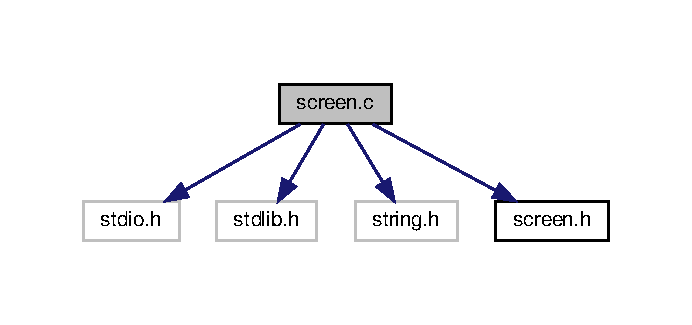
\includegraphics[width=332pt]{screen_8c__incl}
\end{center}
\end{figure}
\subsection*{Data Structures}
\begin{DoxyCompactItemize}
\item 
struct \hyperlink{struct__Area}{\+\_\+\+Area}
\begin{DoxyCompactList}\small\item\em structure of area \end{DoxyCompactList}\end{DoxyCompactItemize}
\subsection*{Macros}
\begin{DoxyCompactItemize}
\item 
\#define \hyperlink{screen_8c_a3cfd3aa62338d12609f6d65bce97e9cd}{R\+O\+WS}~26
\begin{DoxyCompactList}\small\item\em It defines commands. \end{DoxyCompactList}\item 
\mbox{\Hypertarget{screen_8c_a06c6c391fc11d106e9909f0401b255b1}\label{screen_8c_a06c6c391fc11d106e9909f0401b255b1}} 
\#define \hyperlink{screen_8c_a06c6c391fc11d106e9909f0401b255b1}{C\+O\+L\+U\+M\+NS}~80
\begin{DoxyCompactList}\small\item\em It defines number of colums. \end{DoxyCompactList}\item 
\mbox{\Hypertarget{screen_8c_afba5c5b9f73273ce653f890bb64740b0}\label{screen_8c_afba5c5b9f73273ce653f890bb64740b0}} 
\#define \hyperlink{screen_8c_afba5c5b9f73273ce653f890bb64740b0}{T\+O\+T\+A\+L\+\_\+\+D\+A\+TA}~(\hyperlink{screen_8c_a3cfd3aa62338d12609f6d65bce97e9cd}{R\+O\+WS} $\ast$ \hyperlink{screen_8c_a06c6c391fc11d106e9909f0401b255b1}{C\+O\+L\+U\+M\+NS}) + 1
\begin{DoxyCompactList}\small\item\em It defines number of total data. \end{DoxyCompactList}\item 
\mbox{\Hypertarget{screen_8c_a5e7c78a2c827b39d4464f2fc84058f87}\label{screen_8c_a5e7c78a2c827b39d4464f2fc84058f87}} 
\#define \hyperlink{screen_8c_a5e7c78a2c827b39d4464f2fc84058f87}{B\+G\+\_\+\+C\+H\+AR}~\textquotesingle{}$\sim$\textquotesingle{}
\begin{DoxyCompactList}\small\item\em It defines $\sim$. \end{DoxyCompactList}\item 
\mbox{\Hypertarget{screen_8c_a0bbf43d51e6cd6f7119cf1d0063a3a94}\label{screen_8c_a0bbf43d51e6cd6f7119cf1d0063a3a94}} 
\#define \hyperlink{screen_8c_a0bbf43d51e6cd6f7119cf1d0063a3a94}{F\+G\+\_\+\+C\+H\+AR}~\textquotesingle{} \textquotesingle{}
\begin{DoxyCompactList}\small\item\em It defines space. \end{DoxyCompactList}\item 
\mbox{\Hypertarget{screen_8c_accdbea14ea06c15e271784368bd993e8}\label{screen_8c_accdbea14ea06c15e271784368bd993e8}} 
\#define \hyperlink{screen_8c_accdbea14ea06c15e271784368bd993e8}{P\+R\+O\+M\+PT}~\char`\"{} prompt\+:$>$ \char`\"{}
\begin{DoxyCompactList}\small\item\em It defines prompt. \end{DoxyCompactList}\item 
\mbox{\Hypertarget{screen_8c_a28b37557462b06fbb08e707dc0ba2136}\label{screen_8c_a28b37557462b06fbb08e707dc0ba2136}} 
\#define \hyperlink{screen_8c_a28b37557462b06fbb08e707dc0ba2136}{A\+C\+C\+E\+SS}(d,  x,  y)~(d + ((y) $\ast$ \hyperlink{screen_8c_a06c6c391fc11d106e9909f0401b255b1}{C\+O\+L\+U\+M\+NS}) + (x))
\begin{DoxyCompactList}\small\item\em It defines access. \end{DoxyCompactList}\end{DoxyCompactItemize}
\subsection*{Functions}
\begin{DoxyCompactItemize}
\item 
int \hyperlink{screen_8c_ad1b32d3d54fea228f1ef0c73de4a3929}{screen\+\_\+area\+\_\+cursor\+\_\+is\+\_\+out\+\_\+of\+\_\+bounds} (\hyperlink{screen_8h_acfdfc42f6522d75fa3c16713afde8127}{Area} $\ast$area)
\begin{DoxyCompactList}\small\item\em screen area cursor of bounds \end{DoxyCompactList}\item 
void \hyperlink{screen_8c_a110e0b378730322f5a2f1dc91e65e2aa}{screen\+\_\+area\+\_\+scroll\+\_\+up} (\hyperlink{screen_8h_acfdfc42f6522d75fa3c16713afde8127}{Area} $\ast$area)
\begin{DoxyCompactList}\small\item\em screen area scroll up \end{DoxyCompactList}\item 
void \hyperlink{screen_8c_a55dedaa3b402fef825ceb6c3a957781d}{screen\+\_\+utils\+\_\+replaces\+\_\+special\+\_\+chars} (char $\ast$str)
\begin{DoxyCompactList}\small\item\em replaces special characters \end{DoxyCompactList}\item 
void \hyperlink{screen_8c_a9dbb6c251337c03c078dc330caee48d2}{screen\+\_\+init} ()
\begin{DoxyCompactList}\small\item\em screen inicialiciation \end{DoxyCompactList}\item 
void \hyperlink{screen_8c_a3d6d82dde2bb4f3ddc4d276dabe313ef}{screen\+\_\+destroy} ()
\begin{DoxyCompactList}\small\item\em destroy area \end{DoxyCompactList}\item 
void \hyperlink{screen_8c_a3eaa0547a956d39b6c55c9593524e0d1}{screen\+\_\+paint} ()
\begin{DoxyCompactList}\small\item\em screen paints \end{DoxyCompactList}\item 
void \hyperlink{screen_8c_a57b2f852be623dca59255306c1482eb2}{screen\+\_\+gets} (char $\ast$str)
\begin{DoxyCompactList}\small\item\em screen gets \end{DoxyCompactList}\item 
\hyperlink{screen_8h_acfdfc42f6522d75fa3c16713afde8127}{Area} $\ast$ \hyperlink{screen_8c_a194528bec3ed3b57618a8f2df9bea743}{screen\+\_\+area\+\_\+init} (int x, int y, int width, int height)
\begin{DoxyCompactList}\small\item\em inicial area \end{DoxyCompactList}\item 
void \hyperlink{screen_8c_aca5123ed5a7afb75e79c0001e5d1df4f}{screen\+\_\+area\+\_\+destroy} (\hyperlink{screen_8h_acfdfc42f6522d75fa3c16713afde8127}{Area} $\ast$area)
\begin{DoxyCompactList}\small\item\em destroy area \end{DoxyCompactList}\item 
void \hyperlink{screen_8c_a0950dc68cba3d491b909a8abaac1c666}{screen\+\_\+area\+\_\+clear} (\hyperlink{screen_8h_acfdfc42f6522d75fa3c16713afde8127}{Area} $\ast$area)
\begin{DoxyCompactList}\small\item\em clear area \end{DoxyCompactList}\item 
void \hyperlink{screen_8c_af77fa9df4f7170e1e3bf1c6209b7f0c2}{screen\+\_\+area\+\_\+reset\+\_\+cursor} (\hyperlink{screen_8h_acfdfc42f6522d75fa3c16713afde8127}{Area} $\ast$area)
\begin{DoxyCompactList}\small\item\em reset cursor \end{DoxyCompactList}\item 
void \hyperlink{screen_8c_a4f4cd4c7899c096d6c90cc33de9a9814}{screen\+\_\+area\+\_\+puts} (\hyperlink{screen_8h_acfdfc42f6522d75fa3c16713afde8127}{Area} $\ast$area, char $\ast$str)
\begin{DoxyCompactList}\small\item\em puts area \end{DoxyCompactList}\end{DoxyCompactItemize}
\subsection*{Variables}
\begin{DoxyCompactItemize}
\item 
\mbox{\Hypertarget{screen_8c_a34a5b96f7a2aa5db335b9fd09706cf0a}\label{screen_8c_a34a5b96f7a2aa5db335b9fd09706cf0a}} 
char $\ast$ \hyperlink{screen_8c_a34a5b96f7a2aa5db335b9fd09706cf0a}{\+\_\+\+\_\+data}
\begin{DoxyCompactList}\small\item\em It defines variable data. \end{DoxyCompactList}\end{DoxyCompactItemize}


\subsection{Detailed Description}
It defines a screen. 

\begin{DoxyAuthor}{Author}
\end{DoxyAuthor}
\begin{DoxyVersion}{Version}
1.\+0 
\end{DoxyVersion}
\begin{DoxyDate}{Date}
04-\/02-\/2019 
\end{DoxyDate}
\begin{DoxyCopyright}{Copyright}
G\+NU Public License 
\end{DoxyCopyright}


\subsection{Macro Definition Documentation}
\mbox{\Hypertarget{screen_8c_a3cfd3aa62338d12609f6d65bce97e9cd}\label{screen_8c_a3cfd3aa62338d12609f6d65bce97e9cd}} 
\index{screen.\+c@{screen.\+c}!R\+O\+WS@{R\+O\+WS}}
\index{R\+O\+WS@{R\+O\+WS}!screen.\+c@{screen.\+c}}
\subsubsection{\texorpdfstring{R\+O\+WS}{ROWS}}
{\footnotesize\ttfamily \#define R\+O\+WS~26}



It defines commands. 

It defines number of rows 

\subsection{Function Documentation}
\mbox{\Hypertarget{screen_8c_a0950dc68cba3d491b909a8abaac1c666}\label{screen_8c_a0950dc68cba3d491b909a8abaac1c666}} 
\index{screen.\+c@{screen.\+c}!screen\+\_\+area\+\_\+clear@{screen\+\_\+area\+\_\+clear}}
\index{screen\+\_\+area\+\_\+clear@{screen\+\_\+area\+\_\+clear}!screen.\+c@{screen.\+c}}
\subsubsection{\texorpdfstring{screen\+\_\+area\+\_\+clear()}{screen\_area\_clear()}}
{\footnotesize\ttfamily void screen\+\_\+area\+\_\+clear (\begin{DoxyParamCaption}\item[{\hyperlink{screen_8h_acfdfc42f6522d75fa3c16713afde8127}{Area} $\ast$}]{area }\end{DoxyParamCaption})}



clear area 


\begin{DoxyParams}{Parameters}
{\em area} & \\
\hline
\end{DoxyParams}
\begin{DoxyReturn}{Returns}
void 
\end{DoxyReturn}
\mbox{\Hypertarget{screen_8c_ad1b32d3d54fea228f1ef0c73de4a3929}\label{screen_8c_ad1b32d3d54fea228f1ef0c73de4a3929}} 
\index{screen.\+c@{screen.\+c}!screen\+\_\+area\+\_\+cursor\+\_\+is\+\_\+out\+\_\+of\+\_\+bounds@{screen\+\_\+area\+\_\+cursor\+\_\+is\+\_\+out\+\_\+of\+\_\+bounds}}
\index{screen\+\_\+area\+\_\+cursor\+\_\+is\+\_\+out\+\_\+of\+\_\+bounds@{screen\+\_\+area\+\_\+cursor\+\_\+is\+\_\+out\+\_\+of\+\_\+bounds}!screen.\+c@{screen.\+c}}
\subsubsection{\texorpdfstring{screen\+\_\+area\+\_\+cursor\+\_\+is\+\_\+out\+\_\+of\+\_\+bounds()}{screen\_area\_cursor\_is\_out\_of\_bounds()}}
{\footnotesize\ttfamily int screen\+\_\+area\+\_\+cursor\+\_\+is\+\_\+out\+\_\+of\+\_\+bounds (\begin{DoxyParamCaption}\item[{\hyperlink{screen_8h_acfdfc42f6522d75fa3c16713afde8127}{Area} $\ast$}]{area }\end{DoxyParamCaption})}



screen area cursor of bounds 


\begin{DoxyParams}{Parameters}
{\em area} & \\
\hline
\end{DoxyParams}
\begin{DoxyReturn}{Returns}
integer 
\end{DoxyReturn}
\mbox{\Hypertarget{screen_8c_aca5123ed5a7afb75e79c0001e5d1df4f}\label{screen_8c_aca5123ed5a7afb75e79c0001e5d1df4f}} 
\index{screen.\+c@{screen.\+c}!screen\+\_\+area\+\_\+destroy@{screen\+\_\+area\+\_\+destroy}}
\index{screen\+\_\+area\+\_\+destroy@{screen\+\_\+area\+\_\+destroy}!screen.\+c@{screen.\+c}}
\subsubsection{\texorpdfstring{screen\+\_\+area\+\_\+destroy()}{screen\_area\_destroy()}}
{\footnotesize\ttfamily void screen\+\_\+area\+\_\+destroy (\begin{DoxyParamCaption}\item[{\hyperlink{screen_8h_acfdfc42f6522d75fa3c16713afde8127}{Area} $\ast$}]{area }\end{DoxyParamCaption})}



destroy area 


\begin{DoxyParams}{Parameters}
{\em area} & \\
\hline
\end{DoxyParams}
\begin{DoxyReturn}{Returns}
area, in case of error N\+U\+LL 
\end{DoxyReturn}
\mbox{\Hypertarget{screen_8c_a194528bec3ed3b57618a8f2df9bea743}\label{screen_8c_a194528bec3ed3b57618a8f2df9bea743}} 
\index{screen.\+c@{screen.\+c}!screen\+\_\+area\+\_\+init@{screen\+\_\+area\+\_\+init}}
\index{screen\+\_\+area\+\_\+init@{screen\+\_\+area\+\_\+init}!screen.\+c@{screen.\+c}}
\subsubsection{\texorpdfstring{screen\+\_\+area\+\_\+init()}{screen\_area\_init()}}
{\footnotesize\ttfamily \hyperlink{screen_8h_acfdfc42f6522d75fa3c16713afde8127}{Area}$\ast$ screen\+\_\+area\+\_\+init (\begin{DoxyParamCaption}\item[{int}]{x,  }\item[{int}]{y,  }\item[{int}]{width,  }\item[{int}]{height }\end{DoxyParamCaption})}



inicial area 


\begin{DoxyParams}{Parameters}
{\em x} & \\
\hline
{\em y} & \\
\hline
{\em width} & \\
\hline
{\em height} & \\
\hline
\end{DoxyParams}
\begin{DoxyReturn}{Returns}
area 
\end{DoxyReturn}
\mbox{\Hypertarget{screen_8c_a4f4cd4c7899c096d6c90cc33de9a9814}\label{screen_8c_a4f4cd4c7899c096d6c90cc33de9a9814}} 
\index{screen.\+c@{screen.\+c}!screen\+\_\+area\+\_\+puts@{screen\+\_\+area\+\_\+puts}}
\index{screen\+\_\+area\+\_\+puts@{screen\+\_\+area\+\_\+puts}!screen.\+c@{screen.\+c}}
\subsubsection{\texorpdfstring{screen\+\_\+area\+\_\+puts()}{screen\_area\_puts()}}
{\footnotesize\ttfamily void screen\+\_\+area\+\_\+puts (\begin{DoxyParamCaption}\item[{\hyperlink{screen_8h_acfdfc42f6522d75fa3c16713afde8127}{Area} $\ast$}]{area,  }\item[{char $\ast$}]{str }\end{DoxyParamCaption})}



puts area 


\begin{DoxyParams}{Parameters}
{\em area} & \\
\hline
{\em str} & \\
\hline
\end{DoxyParams}
\begin{DoxyReturn}{Returns}
void 
\end{DoxyReturn}
\mbox{\Hypertarget{screen_8c_af77fa9df4f7170e1e3bf1c6209b7f0c2}\label{screen_8c_af77fa9df4f7170e1e3bf1c6209b7f0c2}} 
\index{screen.\+c@{screen.\+c}!screen\+\_\+area\+\_\+reset\+\_\+cursor@{screen\+\_\+area\+\_\+reset\+\_\+cursor}}
\index{screen\+\_\+area\+\_\+reset\+\_\+cursor@{screen\+\_\+area\+\_\+reset\+\_\+cursor}!screen.\+c@{screen.\+c}}
\subsubsection{\texorpdfstring{screen\+\_\+area\+\_\+reset\+\_\+cursor()}{screen\_area\_reset\_cursor()}}
{\footnotesize\ttfamily void screen\+\_\+area\+\_\+reset\+\_\+cursor (\begin{DoxyParamCaption}\item[{\hyperlink{screen_8h_acfdfc42f6522d75fa3c16713afde8127}{Area} $\ast$}]{area }\end{DoxyParamCaption})}



reset cursor 


\begin{DoxyParams}{Parameters}
{\em area} & \\
\hline
\end{DoxyParams}
\begin{DoxyReturn}{Returns}
void 
\end{DoxyReturn}
\mbox{\Hypertarget{screen_8c_a110e0b378730322f5a2f1dc91e65e2aa}\label{screen_8c_a110e0b378730322f5a2f1dc91e65e2aa}} 
\index{screen.\+c@{screen.\+c}!screen\+\_\+area\+\_\+scroll\+\_\+up@{screen\+\_\+area\+\_\+scroll\+\_\+up}}
\index{screen\+\_\+area\+\_\+scroll\+\_\+up@{screen\+\_\+area\+\_\+scroll\+\_\+up}!screen.\+c@{screen.\+c}}
\subsubsection{\texorpdfstring{screen\+\_\+area\+\_\+scroll\+\_\+up()}{screen\_area\_scroll\_up()}}
{\footnotesize\ttfamily void screen\+\_\+area\+\_\+scroll\+\_\+up (\begin{DoxyParamCaption}\item[{\hyperlink{screen_8h_acfdfc42f6522d75fa3c16713afde8127}{Area} $\ast$}]{area }\end{DoxyParamCaption})}



screen area scroll up 


\begin{DoxyParams}{Parameters}
{\em area} & \\
\hline
\end{DoxyParams}
\begin{DoxyReturn}{Returns}
void 
\end{DoxyReturn}
\mbox{\Hypertarget{screen_8c_a3d6d82dde2bb4f3ddc4d276dabe313ef}\label{screen_8c_a3d6d82dde2bb4f3ddc4d276dabe313ef}} 
\index{screen.\+c@{screen.\+c}!screen\+\_\+destroy@{screen\+\_\+destroy}}
\index{screen\+\_\+destroy@{screen\+\_\+destroy}!screen.\+c@{screen.\+c}}
\subsubsection{\texorpdfstring{screen\+\_\+destroy()}{screen\_destroy()}}
{\footnotesize\ttfamily void screen\+\_\+destroy (\begin{DoxyParamCaption}{ }\end{DoxyParamCaption})}



destroy area 

\begin{DoxyReturn}{Returns}

\end{DoxyReturn}
\mbox{\Hypertarget{screen_8c_a57b2f852be623dca59255306c1482eb2}\label{screen_8c_a57b2f852be623dca59255306c1482eb2}} 
\index{screen.\+c@{screen.\+c}!screen\+\_\+gets@{screen\+\_\+gets}}
\index{screen\+\_\+gets@{screen\+\_\+gets}!screen.\+c@{screen.\+c}}
\subsubsection{\texorpdfstring{screen\+\_\+gets()}{screen\_gets()}}
{\footnotesize\ttfamily void screen\+\_\+gets (\begin{DoxyParamCaption}\item[{char $\ast$}]{str }\end{DoxyParamCaption})}



screen gets 


\begin{DoxyParams}{Parameters}
{\em str} & \\
\hline
\end{DoxyParams}
\begin{DoxyReturn}{Returns}
void 
\end{DoxyReturn}
\mbox{\Hypertarget{screen_8c_a9dbb6c251337c03c078dc330caee48d2}\label{screen_8c_a9dbb6c251337c03c078dc330caee48d2}} 
\index{screen.\+c@{screen.\+c}!screen\+\_\+init@{screen\+\_\+init}}
\index{screen\+\_\+init@{screen\+\_\+init}!screen.\+c@{screen.\+c}}
\subsubsection{\texorpdfstring{screen\+\_\+init()}{screen\_init()}}
{\footnotesize\ttfamily void screen\+\_\+init (\begin{DoxyParamCaption}{ }\end{DoxyParamCaption})}



screen inicialiciation 

\begin{DoxyReturn}{Returns}
void 
\end{DoxyReturn}
\mbox{\Hypertarget{screen_8c_a3eaa0547a956d39b6c55c9593524e0d1}\label{screen_8c_a3eaa0547a956d39b6c55c9593524e0d1}} 
\index{screen.\+c@{screen.\+c}!screen\+\_\+paint@{screen\+\_\+paint}}
\index{screen\+\_\+paint@{screen\+\_\+paint}!screen.\+c@{screen.\+c}}
\subsubsection{\texorpdfstring{screen\+\_\+paint()}{screen\_paint()}}
{\footnotesize\ttfamily void screen\+\_\+paint (\begin{DoxyParamCaption}{ }\end{DoxyParamCaption})}



screen paints 

\begin{DoxyReturn}{Returns}
void 
\end{DoxyReturn}
\mbox{\Hypertarget{screen_8c_a55dedaa3b402fef825ceb6c3a957781d}\label{screen_8c_a55dedaa3b402fef825ceb6c3a957781d}} 
\index{screen.\+c@{screen.\+c}!screen\+\_\+utils\+\_\+replaces\+\_\+special\+\_\+chars@{screen\+\_\+utils\+\_\+replaces\+\_\+special\+\_\+chars}}
\index{screen\+\_\+utils\+\_\+replaces\+\_\+special\+\_\+chars@{screen\+\_\+utils\+\_\+replaces\+\_\+special\+\_\+chars}!screen.\+c@{screen.\+c}}
\subsubsection{\texorpdfstring{screen\+\_\+utils\+\_\+replaces\+\_\+special\+\_\+chars()}{screen\_utils\_replaces\_special\_chars()}}
{\footnotesize\ttfamily void screen\+\_\+utils\+\_\+replaces\+\_\+special\+\_\+chars (\begin{DoxyParamCaption}\item[{char $\ast$}]{str }\end{DoxyParamCaption})}



replaces special characters 


\begin{DoxyParams}{Parameters}
{\em str} & \\
\hline
\end{DoxyParams}
\begin{DoxyReturn}{Returns}
void 
\end{DoxyReturn}


\hypertarget{screen_8h}{}\section{screen.\+h File Reference}
\label{screen_8h}\index{screen.\+h@{screen.\+h}}


It defines a screen.  


This graph shows which files directly or indirectly include this file\+:
\nopagebreak
\begin{figure}[H]
\begin{center}
\leavevmode
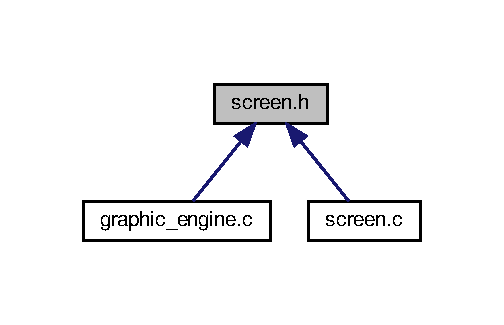
\includegraphics[width=242pt]{screen_8h__dep__incl}
\end{center}
\end{figure}
\subsection*{Macros}
\begin{DoxyCompactItemize}
\item 
\mbox{\Hypertarget{screen_8h_aab63df3ae7b979d59ea0188055ea0763}\label{screen_8h_aab63df3ae7b979d59ea0188055ea0763}} 
\#define \hyperlink{screen_8h_aab63df3ae7b979d59ea0188055ea0763}{S\+C\+R\+E\+E\+N\+\_\+\+M\+A\+X\+\_\+\+S\+TR}~80
\begin{DoxyCompactList}\small\item\em defines the max number of screen \end{DoxyCompactList}\end{DoxyCompactItemize}
\subsection*{Typedefs}
\begin{DoxyCompactItemize}
\item 
\mbox{\Hypertarget{screen_8h_acfdfc42f6522d75fa3c16713afde8127}\label{screen_8h_acfdfc42f6522d75fa3c16713afde8127}} 
typedef struct \hyperlink{struct__Area}{\+\_\+\+Area} \hyperlink{screen_8h_acfdfc42f6522d75fa3c16713afde8127}{Area}
\begin{DoxyCompactList}\small\item\em defines the Object structure \end{DoxyCompactList}\end{DoxyCompactItemize}
\subsection*{Functions}
\begin{DoxyCompactItemize}
\item 
void \hyperlink{screen_8h_a9dbb6c251337c03c078dc330caee48d2}{screen\+\_\+init} ()
\begin{DoxyCompactList}\small\item\em screen inicialiciation \end{DoxyCompactList}\item 
void \hyperlink{screen_8h_a3d6d82dde2bb4f3ddc4d276dabe313ef}{screen\+\_\+destroy} ()
\begin{DoxyCompactList}\small\item\em destroy area \end{DoxyCompactList}\item 
void \hyperlink{screen_8h_a3eaa0547a956d39b6c55c9593524e0d1}{screen\+\_\+paint} ()
\begin{DoxyCompactList}\small\item\em screen paints \end{DoxyCompactList}\item 
void \hyperlink{screen_8h_a57b2f852be623dca59255306c1482eb2}{screen\+\_\+gets} (char $\ast$str)
\begin{DoxyCompactList}\small\item\em screen gets \end{DoxyCompactList}\item 
\hyperlink{screen_8h_acfdfc42f6522d75fa3c16713afde8127}{Area} $\ast$ \hyperlink{screen_8h_a194528bec3ed3b57618a8f2df9bea743}{screen\+\_\+area\+\_\+init} (int x, int y, int width, int height)
\begin{DoxyCompactList}\small\item\em inicial area \end{DoxyCompactList}\item 
void \hyperlink{screen_8h_aca5123ed5a7afb75e79c0001e5d1df4f}{screen\+\_\+area\+\_\+destroy} (\hyperlink{screen_8h_acfdfc42f6522d75fa3c16713afde8127}{Area} $\ast$area)
\begin{DoxyCompactList}\small\item\em destroy area \end{DoxyCompactList}\item 
void \hyperlink{screen_8h_a0950dc68cba3d491b909a8abaac1c666}{screen\+\_\+area\+\_\+clear} (\hyperlink{screen_8h_acfdfc42f6522d75fa3c16713afde8127}{Area} $\ast$area)
\begin{DoxyCompactList}\small\item\em clear area \end{DoxyCompactList}\item 
void \hyperlink{screen_8h_af77fa9df4f7170e1e3bf1c6209b7f0c2}{screen\+\_\+area\+\_\+reset\+\_\+cursor} (\hyperlink{screen_8h_acfdfc42f6522d75fa3c16713afde8127}{Area} $\ast$area)
\begin{DoxyCompactList}\small\item\em reset cursor \end{DoxyCompactList}\item 
void \hyperlink{screen_8h_a4f4cd4c7899c096d6c90cc33de9a9814}{screen\+\_\+area\+\_\+puts} (\hyperlink{screen_8h_acfdfc42f6522d75fa3c16713afde8127}{Area} $\ast$area, char $\ast$str)
\begin{DoxyCompactList}\small\item\em puts area \end{DoxyCompactList}\end{DoxyCompactItemize}


\subsection{Detailed Description}
It defines a screen. 

\begin{DoxyAuthor}{Author}
\end{DoxyAuthor}
\begin{DoxyVersion}{Version}
1.\+0 
\end{DoxyVersion}
\begin{DoxyDate}{Date}
04-\/02-\/2019 
\end{DoxyDate}
\begin{DoxyCopyright}{Copyright}
G\+NU Public License 
\end{DoxyCopyright}


\subsection{Function Documentation}
\mbox{\Hypertarget{screen_8h_a0950dc68cba3d491b909a8abaac1c666}\label{screen_8h_a0950dc68cba3d491b909a8abaac1c666}} 
\index{screen.\+h@{screen.\+h}!screen\+\_\+area\+\_\+clear@{screen\+\_\+area\+\_\+clear}}
\index{screen\+\_\+area\+\_\+clear@{screen\+\_\+area\+\_\+clear}!screen.\+h@{screen.\+h}}
\subsubsection{\texorpdfstring{screen\+\_\+area\+\_\+clear()}{screen\_area\_clear()}}
{\footnotesize\ttfamily void screen\+\_\+area\+\_\+clear (\begin{DoxyParamCaption}\item[{\hyperlink{screen_8h_acfdfc42f6522d75fa3c16713afde8127}{Area} $\ast$}]{area }\end{DoxyParamCaption})}



clear area 


\begin{DoxyParams}{Parameters}
{\em area} & \\
\hline
\end{DoxyParams}
\begin{DoxyReturn}{Returns}
void 
\end{DoxyReturn}
\mbox{\Hypertarget{screen_8h_aca5123ed5a7afb75e79c0001e5d1df4f}\label{screen_8h_aca5123ed5a7afb75e79c0001e5d1df4f}} 
\index{screen.\+h@{screen.\+h}!screen\+\_\+area\+\_\+destroy@{screen\+\_\+area\+\_\+destroy}}
\index{screen\+\_\+area\+\_\+destroy@{screen\+\_\+area\+\_\+destroy}!screen.\+h@{screen.\+h}}
\subsubsection{\texorpdfstring{screen\+\_\+area\+\_\+destroy()}{screen\_area\_destroy()}}
{\footnotesize\ttfamily void screen\+\_\+area\+\_\+destroy (\begin{DoxyParamCaption}\item[{\hyperlink{screen_8h_acfdfc42f6522d75fa3c16713afde8127}{Area} $\ast$}]{area }\end{DoxyParamCaption})}



destroy area 


\begin{DoxyParams}{Parameters}
{\em area} & \\
\hline
\end{DoxyParams}
\begin{DoxyReturn}{Returns}
area, in case of error N\+U\+LL 
\end{DoxyReturn}
\mbox{\Hypertarget{screen_8h_a194528bec3ed3b57618a8f2df9bea743}\label{screen_8h_a194528bec3ed3b57618a8f2df9bea743}} 
\index{screen.\+h@{screen.\+h}!screen\+\_\+area\+\_\+init@{screen\+\_\+area\+\_\+init}}
\index{screen\+\_\+area\+\_\+init@{screen\+\_\+area\+\_\+init}!screen.\+h@{screen.\+h}}
\subsubsection{\texorpdfstring{screen\+\_\+area\+\_\+init()}{screen\_area\_init()}}
{\footnotesize\ttfamily \hyperlink{screen_8h_acfdfc42f6522d75fa3c16713afde8127}{Area}$\ast$ screen\+\_\+area\+\_\+init (\begin{DoxyParamCaption}\item[{int}]{x,  }\item[{int}]{y,  }\item[{int}]{width,  }\item[{int}]{height }\end{DoxyParamCaption})}



inicial area 


\begin{DoxyParams}{Parameters}
{\em x} & \\
\hline
{\em y} & \\
\hline
{\em width} & \\
\hline
{\em height} & \\
\hline
\end{DoxyParams}
\begin{DoxyReturn}{Returns}
area 
\end{DoxyReturn}
\mbox{\Hypertarget{screen_8h_a4f4cd4c7899c096d6c90cc33de9a9814}\label{screen_8h_a4f4cd4c7899c096d6c90cc33de9a9814}} 
\index{screen.\+h@{screen.\+h}!screen\+\_\+area\+\_\+puts@{screen\+\_\+area\+\_\+puts}}
\index{screen\+\_\+area\+\_\+puts@{screen\+\_\+area\+\_\+puts}!screen.\+h@{screen.\+h}}
\subsubsection{\texorpdfstring{screen\+\_\+area\+\_\+puts()}{screen\_area\_puts()}}
{\footnotesize\ttfamily void screen\+\_\+area\+\_\+puts (\begin{DoxyParamCaption}\item[{\hyperlink{screen_8h_acfdfc42f6522d75fa3c16713afde8127}{Area} $\ast$}]{area,  }\item[{char $\ast$}]{str }\end{DoxyParamCaption})}



puts area 


\begin{DoxyParams}{Parameters}
{\em area} & \\
\hline
{\em str} & \\
\hline
\end{DoxyParams}
\begin{DoxyReturn}{Returns}
void 
\end{DoxyReturn}
\mbox{\Hypertarget{screen_8h_af77fa9df4f7170e1e3bf1c6209b7f0c2}\label{screen_8h_af77fa9df4f7170e1e3bf1c6209b7f0c2}} 
\index{screen.\+h@{screen.\+h}!screen\+\_\+area\+\_\+reset\+\_\+cursor@{screen\+\_\+area\+\_\+reset\+\_\+cursor}}
\index{screen\+\_\+area\+\_\+reset\+\_\+cursor@{screen\+\_\+area\+\_\+reset\+\_\+cursor}!screen.\+h@{screen.\+h}}
\subsubsection{\texorpdfstring{screen\+\_\+area\+\_\+reset\+\_\+cursor()}{screen\_area\_reset\_cursor()}}
{\footnotesize\ttfamily void screen\+\_\+area\+\_\+reset\+\_\+cursor (\begin{DoxyParamCaption}\item[{\hyperlink{screen_8h_acfdfc42f6522d75fa3c16713afde8127}{Area} $\ast$}]{area }\end{DoxyParamCaption})}



reset cursor 


\begin{DoxyParams}{Parameters}
{\em area} & \\
\hline
\end{DoxyParams}
\begin{DoxyReturn}{Returns}
void 
\end{DoxyReturn}
\mbox{\Hypertarget{screen_8h_a3d6d82dde2bb4f3ddc4d276dabe313ef}\label{screen_8h_a3d6d82dde2bb4f3ddc4d276dabe313ef}} 
\index{screen.\+h@{screen.\+h}!screen\+\_\+destroy@{screen\+\_\+destroy}}
\index{screen\+\_\+destroy@{screen\+\_\+destroy}!screen.\+h@{screen.\+h}}
\subsubsection{\texorpdfstring{screen\+\_\+destroy()}{screen\_destroy()}}
{\footnotesize\ttfamily void screen\+\_\+destroy (\begin{DoxyParamCaption}{ }\end{DoxyParamCaption})}



destroy area 

\begin{DoxyReturn}{Returns}

\end{DoxyReturn}
\mbox{\Hypertarget{screen_8h_a57b2f852be623dca59255306c1482eb2}\label{screen_8h_a57b2f852be623dca59255306c1482eb2}} 
\index{screen.\+h@{screen.\+h}!screen\+\_\+gets@{screen\+\_\+gets}}
\index{screen\+\_\+gets@{screen\+\_\+gets}!screen.\+h@{screen.\+h}}
\subsubsection{\texorpdfstring{screen\+\_\+gets()}{screen\_gets()}}
{\footnotesize\ttfamily void screen\+\_\+gets (\begin{DoxyParamCaption}\item[{char $\ast$}]{str }\end{DoxyParamCaption})}



screen gets 


\begin{DoxyParams}{Parameters}
{\em str} & \\
\hline
\end{DoxyParams}
\begin{DoxyReturn}{Returns}
void 
\end{DoxyReturn}
\mbox{\Hypertarget{screen_8h_a9dbb6c251337c03c078dc330caee48d2}\label{screen_8h_a9dbb6c251337c03c078dc330caee48d2}} 
\index{screen.\+h@{screen.\+h}!screen\+\_\+init@{screen\+\_\+init}}
\index{screen\+\_\+init@{screen\+\_\+init}!screen.\+h@{screen.\+h}}
\subsubsection{\texorpdfstring{screen\+\_\+init()}{screen\_init()}}
{\footnotesize\ttfamily void screen\+\_\+init (\begin{DoxyParamCaption}{ }\end{DoxyParamCaption})}



screen inicialiciation 

\begin{DoxyReturn}{Returns}
void 
\end{DoxyReturn}
\mbox{\Hypertarget{screen_8h_a3eaa0547a956d39b6c55c9593524e0d1}\label{screen_8h_a3eaa0547a956d39b6c55c9593524e0d1}} 
\index{screen.\+h@{screen.\+h}!screen\+\_\+paint@{screen\+\_\+paint}}
\index{screen\+\_\+paint@{screen\+\_\+paint}!screen.\+h@{screen.\+h}}
\subsubsection{\texorpdfstring{screen\+\_\+paint()}{screen\_paint()}}
{\footnotesize\ttfamily void screen\+\_\+paint (\begin{DoxyParamCaption}{ }\end{DoxyParamCaption})}



screen paints 

\begin{DoxyReturn}{Returns}
void 
\end{DoxyReturn}


\hypertarget{set_8c}{}\section{set.\+c File Reference}
\label{set_8c}\index{set.\+c@{set.\+c}}


It defines the module S\+ET.  


{\ttfamily \#include $<$stdio.\+h$>$}\newline
{\ttfamily \#include $<$stdlib.\+h$>$}\newline
{\ttfamily \#include $<$string.\+h$>$}\newline
{\ttfamily \#include \char`\"{}object.\+h\char`\"{}}\newline
{\ttfamily \#include \char`\"{}game.\+h\char`\"{}}\newline
{\ttfamily \#include \char`\"{}space.\+h\char`\"{}}\newline
{\ttfamily \#include \char`\"{}types.\+h\char`\"{}}\newline
{\ttfamily \#include \char`\"{}set.\+h\char`\"{}}\newline
Include dependency graph for set.\+c\+:
\nopagebreak
\begin{figure}[H]
\begin{center}
\leavevmode
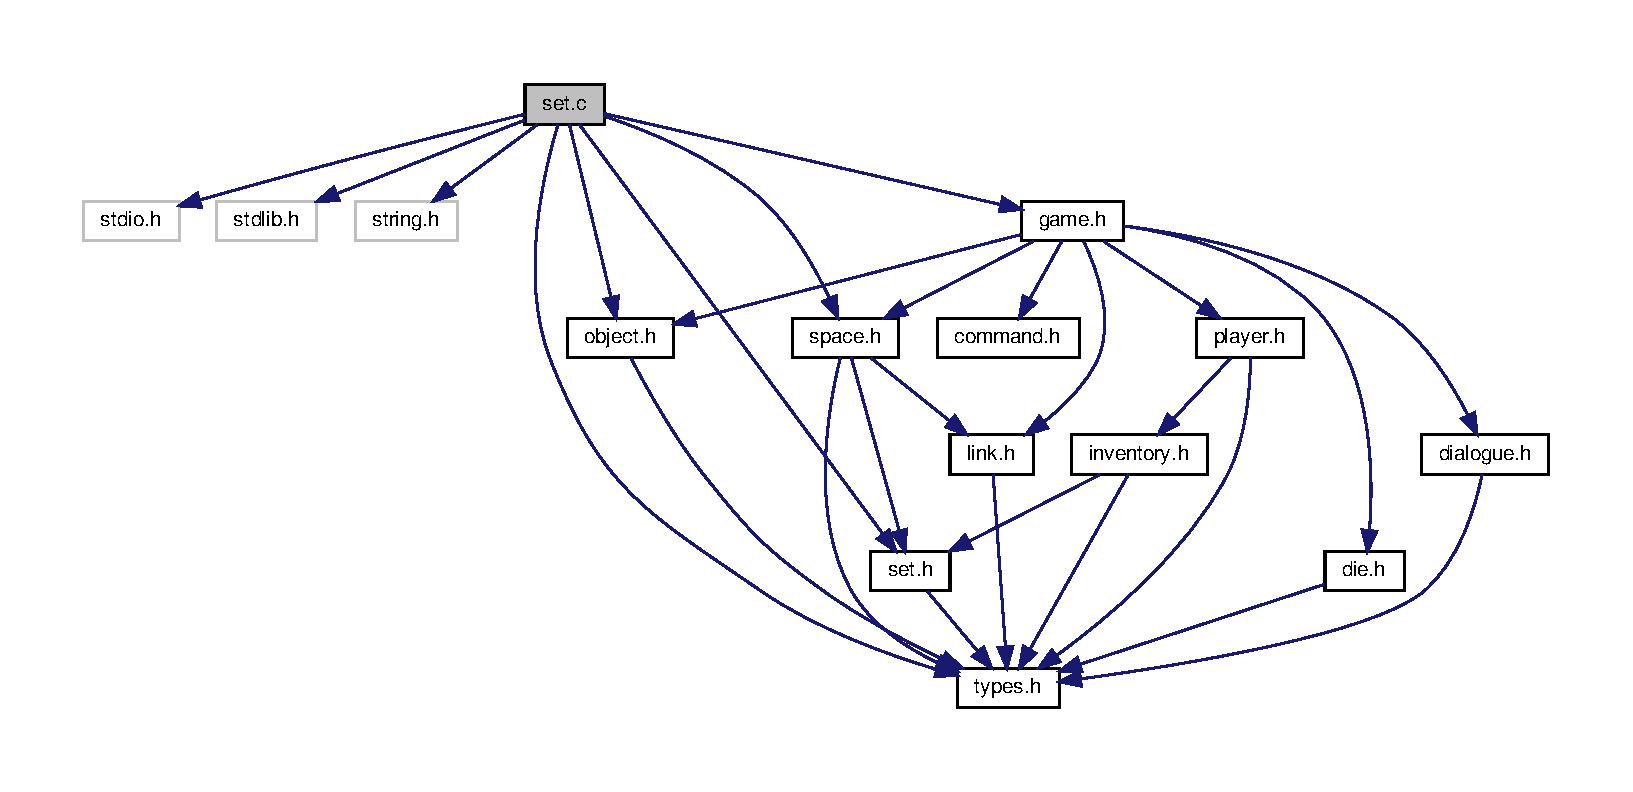
\includegraphics[width=350pt]{set_8c__incl}
\end{center}
\end{figure}
\subsection*{Data Structures}
\begin{DoxyCompactItemize}
\item 
struct \hyperlink{struct__Set}{\+\_\+\+Set}
\begin{DoxyCompactList}\small\item\em defines the structure of set \end{DoxyCompactList}\end{DoxyCompactItemize}
\subsection*{Functions}
\begin{DoxyCompactItemize}
\item 
\hyperlink{set_8h_a6d3b7f7c92cbb4577ef3ef7ddbf93161}{Set} $\ast$ \hyperlink{set_8c_abcc73b7ad3913fc92dd95d366c9c8687}{set\+\_\+create} ()
\begin{DoxyCompactList}\small\item\em create the set in the game \end{DoxyCompactList}\item 
\hyperlink{types_8h_a32c27cc471df37f4fc818d65de0a56c4}{S\+T\+A\+T\+US} \hyperlink{set_8c_a1f3a3f5d74c6dd9e9be0ec515fae282a}{set\+\_\+destroy} (\hyperlink{set_8h_a6d3b7f7c92cbb4577ef3ef7ddbf93161}{Set} $\ast$aux)
\begin{DoxyCompactList}\small\item\em destroy the set in the game \end{DoxyCompactList}\item 
\hyperlink{types_8h_a3e5b8192e7d9ffaf3542f1210aec18dd}{B\+O\+OL} \hyperlink{set_8c_a6426d210af9f56c938fba5f221ec6a80}{set\+\_\+id\+\_\+in} (\hyperlink{set_8h_a6d3b7f7c92cbb4577ef3ef7ddbf93161}{Set} $\ast$aux, \hyperlink{types_8h_a845e604fb28f7e3d97549da3448149d3}{Id} var)
\begin{DoxyCompactList}\small\item\em set the id in the game \end{DoxyCompactList}\item 
\hyperlink{types_8h_a32c27cc471df37f4fc818d65de0a56c4}{S\+T\+A\+T\+US} \hyperlink{set_8c_ab43446d7f625f4b646da3810609ef92d}{set\+\_\+id\+\_\+add} (\hyperlink{set_8h_a6d3b7f7c92cbb4577ef3ef7ddbf93161}{Set} $\ast$aux, \hyperlink{types_8h_a845e604fb28f7e3d97549da3448149d3}{Id} new)
\begin{DoxyCompactList}\small\item\em set the id add in the game \end{DoxyCompactList}\item 
\hyperlink{types_8h_a32c27cc471df37f4fc818d65de0a56c4}{S\+T\+A\+T\+US} \hyperlink{set_8c_a7c68c583fc56840769f93dd8a0e24d8a}{set\+\_\+remov\+\_\+id} (\hyperlink{set_8h_a6d3b7f7c92cbb4577ef3ef7ddbf93161}{Set} $\ast$aux, \hyperlink{types_8h_a845e604fb28f7e3d97549da3448149d3}{Id} rmv)
\begin{DoxyCompactList}\small\item\em remove the id add in the game \end{DoxyCompactList}\item 
\hyperlink{types_8h_a845e604fb28f7e3d97549da3448149d3}{Id} \hyperlink{set_8c_a68b44d04ca0d7ba5b3e949f04dd2f8ff}{set\+\_\+get\+\_\+id} (\hyperlink{set_8h_a6d3b7f7c92cbb4577ef3ef7ddbf93161}{Set} $\ast$aux, int pos)
\begin{DoxyCompactList}\small\item\em set the id add in the game \end{DoxyCompactList}\item 
int \hyperlink{set_8c_a69784555363e44d97c4f6c0119bc52d8}{set\+\_\+get\+Num} (\hyperlink{set_8h_a6d3b7f7c92cbb4577ef3ef7ddbf93161}{Set} $\ast$set)
\begin{DoxyCompactList}\small\item\em set get number in the game \end{DoxyCompactList}\item 
\hyperlink{types_8h_a32c27cc471df37f4fc818d65de0a56c4}{S\+T\+A\+T\+US} \hyperlink{set_8c_afb5717fc0d782e62066cfe40960d5362}{set\+\_\+set\+\_\+id} (\hyperlink{set_8h_a6d3b7f7c92cbb4577ef3ef7ddbf93161}{Set} $\ast$aux, \hyperlink{types_8h_a845e604fb28f7e3d97549da3448149d3}{Id} id, int pos)
\begin{DoxyCompactList}\small\item\em set the id in the game \end{DoxyCompactList}\item 
\hyperlink{types_8h_a32c27cc471df37f4fc818d65de0a56c4}{S\+T\+A\+T\+US} \hyperlink{set_8c_a38ab539c50ee57aae502ee63657bcf22}{set\+\_\+print} (\hyperlink{set_8h_a6d3b7f7c92cbb4577ef3ef7ddbf93161}{Set} $\ast$aux)
\begin{DoxyCompactList}\small\item\em prints the set \end{DoxyCompactList}\end{DoxyCompactItemize}


\subsection{Detailed Description}
It defines the module S\+ET. 

\begin{DoxyAuthor}{Author}
\end{DoxyAuthor}
\begin{DoxyVersion}{Version}
1.\+0 
\end{DoxyVersion}
\begin{DoxyDate}{Date}
21-\/02-\/2019 
\end{DoxyDate}
\begin{DoxyCopyright}{Copyright}
G\+NU Public License 
\end{DoxyCopyright}


\subsection{Function Documentation}
\mbox{\Hypertarget{set_8c_abcc73b7ad3913fc92dd95d366c9c8687}\label{set_8c_abcc73b7ad3913fc92dd95d366c9c8687}} 
\index{set.\+c@{set.\+c}!set\+\_\+create@{set\+\_\+create}}
\index{set\+\_\+create@{set\+\_\+create}!set.\+c@{set.\+c}}
\subsubsection{\texorpdfstring{set\+\_\+create()}{set\_create()}}
{\footnotesize\ttfamily \hyperlink{set_8h_a6d3b7f7c92cbb4577ef3ef7ddbf93161}{Set}$\ast$ set\+\_\+create (\begin{DoxyParamCaption}{ }\end{DoxyParamCaption})}



create the set in the game 

\begin{DoxyReturn}{Returns}
set or in case of error N\+U\+LL 
\end{DoxyReturn}
\mbox{\Hypertarget{set_8c_a1f3a3f5d74c6dd9e9be0ec515fae282a}\label{set_8c_a1f3a3f5d74c6dd9e9be0ec515fae282a}} 
\index{set.\+c@{set.\+c}!set\+\_\+destroy@{set\+\_\+destroy}}
\index{set\+\_\+destroy@{set\+\_\+destroy}!set.\+c@{set.\+c}}
\subsubsection{\texorpdfstring{set\+\_\+destroy()}{set\_destroy()}}
{\footnotesize\ttfamily \hyperlink{types_8h_a32c27cc471df37f4fc818d65de0a56c4}{S\+T\+A\+T\+US} set\+\_\+destroy (\begin{DoxyParamCaption}\item[{\hyperlink{set_8h_a6d3b7f7c92cbb4577ef3ef7ddbf93161}{Set} $\ast$}]{aux }\end{DoxyParamCaption})}



destroy the set in the game 


\begin{DoxyParams}{Parameters}
{\em aux} & \\
\hline
\end{DoxyParams}
\begin{DoxyReturn}{Returns}
OK, or E\+R\+R\+OR 
\end{DoxyReturn}
\mbox{\Hypertarget{set_8c_a68b44d04ca0d7ba5b3e949f04dd2f8ff}\label{set_8c_a68b44d04ca0d7ba5b3e949f04dd2f8ff}} 
\index{set.\+c@{set.\+c}!set\+\_\+get\+\_\+id@{set\+\_\+get\+\_\+id}}
\index{set\+\_\+get\+\_\+id@{set\+\_\+get\+\_\+id}!set.\+c@{set.\+c}}
\subsubsection{\texorpdfstring{set\+\_\+get\+\_\+id()}{set\_get\_id()}}
{\footnotesize\ttfamily \hyperlink{types_8h_a845e604fb28f7e3d97549da3448149d3}{Id} set\+\_\+get\+\_\+id (\begin{DoxyParamCaption}\item[{\hyperlink{set_8h_a6d3b7f7c92cbb4577ef3ef7ddbf93161}{Set} $\ast$}]{aux,  }\item[{int}]{pos }\end{DoxyParamCaption})}



set the id add in the game 


\begin{DoxyParams}{Parameters}
{\em aux} & \\
\hline
{\em pos} & \\
\hline
\end{DoxyParams}
\begin{DoxyReturn}{Returns}
id or in case of error N\+U\+LL 
\end{DoxyReturn}
\mbox{\Hypertarget{set_8c_a69784555363e44d97c4f6c0119bc52d8}\label{set_8c_a69784555363e44d97c4f6c0119bc52d8}} 
\index{set.\+c@{set.\+c}!set\+\_\+get\+Num@{set\+\_\+get\+Num}}
\index{set\+\_\+get\+Num@{set\+\_\+get\+Num}!set.\+c@{set.\+c}}
\subsubsection{\texorpdfstring{set\+\_\+get\+Num()}{set\_getNum()}}
{\footnotesize\ttfamily int set\+\_\+get\+Num (\begin{DoxyParamCaption}\item[{\hyperlink{set_8h_a6d3b7f7c92cbb4577ef3ef7ddbf93161}{Set} $\ast$}]{set }\end{DoxyParamCaption})}



set get number in the game 


\begin{DoxyParams}{Parameters}
{\em set} & \\
\hline
\end{DoxyParams}
\begin{DoxyReturn}{Returns}
number of sets 
\end{DoxyReturn}
\mbox{\Hypertarget{set_8c_ab43446d7f625f4b646da3810609ef92d}\label{set_8c_ab43446d7f625f4b646da3810609ef92d}} 
\index{set.\+c@{set.\+c}!set\+\_\+id\+\_\+add@{set\+\_\+id\+\_\+add}}
\index{set\+\_\+id\+\_\+add@{set\+\_\+id\+\_\+add}!set.\+c@{set.\+c}}
\subsubsection{\texorpdfstring{set\+\_\+id\+\_\+add()}{set\_id\_add()}}
{\footnotesize\ttfamily \hyperlink{types_8h_a32c27cc471df37f4fc818d65de0a56c4}{S\+T\+A\+T\+US} set\+\_\+id\+\_\+add (\begin{DoxyParamCaption}\item[{\hyperlink{set_8h_a6d3b7f7c92cbb4577ef3ef7ddbf93161}{Set} $\ast$}]{aux,  }\item[{\hyperlink{types_8h_a845e604fb28f7e3d97549da3448149d3}{Id}}]{new }\end{DoxyParamCaption})}



set the id add in the game 


\begin{DoxyParams}{Parameters}
{\em aux} & \\
\hline
{\em new} & \\
\hline
\end{DoxyParams}
\begin{DoxyReturn}{Returns}
OK, or E\+R\+R\+OR 
\end{DoxyReturn}
\mbox{\Hypertarget{set_8c_a6426d210af9f56c938fba5f221ec6a80}\label{set_8c_a6426d210af9f56c938fba5f221ec6a80}} 
\index{set.\+c@{set.\+c}!set\+\_\+id\+\_\+in@{set\+\_\+id\+\_\+in}}
\index{set\+\_\+id\+\_\+in@{set\+\_\+id\+\_\+in}!set.\+c@{set.\+c}}
\subsubsection{\texorpdfstring{set\+\_\+id\+\_\+in()}{set\_id\_in()}}
{\footnotesize\ttfamily \hyperlink{types_8h_a3e5b8192e7d9ffaf3542f1210aec18dd}{B\+O\+OL} set\+\_\+id\+\_\+in (\begin{DoxyParamCaption}\item[{\hyperlink{set_8h_a6d3b7f7c92cbb4577ef3ef7ddbf93161}{Set} $\ast$}]{aux,  }\item[{\hyperlink{types_8h_a845e604fb28f7e3d97549da3448149d3}{Id}}]{var }\end{DoxyParamCaption})}



set the id in the game 


\begin{DoxyParams}{Parameters}
{\em aux} & \\
\hline
{\em var} & \\
\hline
\end{DoxyParams}
\begin{DoxyReturn}{Returns}
T\+R\+UE or F\+A\+L\+SE 
\end{DoxyReturn}
\mbox{\Hypertarget{set_8c_a38ab539c50ee57aae502ee63657bcf22}\label{set_8c_a38ab539c50ee57aae502ee63657bcf22}} 
\index{set.\+c@{set.\+c}!set\+\_\+print@{set\+\_\+print}}
\index{set\+\_\+print@{set\+\_\+print}!set.\+c@{set.\+c}}
\subsubsection{\texorpdfstring{set\+\_\+print()}{set\_print()}}
{\footnotesize\ttfamily \hyperlink{types_8h_a32c27cc471df37f4fc818d65de0a56c4}{S\+T\+A\+T\+US} set\+\_\+print (\begin{DoxyParamCaption}\item[{\hyperlink{set_8h_a6d3b7f7c92cbb4577ef3ef7ddbf93161}{Set} $\ast$}]{aux }\end{DoxyParamCaption})}



prints the set 


\begin{DoxyParams}{Parameters}
{\em aux} & \\
\hline
\end{DoxyParams}
\begin{DoxyReturn}{Returns}
OK, or E\+R\+R\+OR 
\end{DoxyReturn}
\mbox{\Hypertarget{set_8c_a7c68c583fc56840769f93dd8a0e24d8a}\label{set_8c_a7c68c583fc56840769f93dd8a0e24d8a}} 
\index{set.\+c@{set.\+c}!set\+\_\+remov\+\_\+id@{set\+\_\+remov\+\_\+id}}
\index{set\+\_\+remov\+\_\+id@{set\+\_\+remov\+\_\+id}!set.\+c@{set.\+c}}
\subsubsection{\texorpdfstring{set\+\_\+remov\+\_\+id()}{set\_remov\_id()}}
{\footnotesize\ttfamily \hyperlink{types_8h_a32c27cc471df37f4fc818d65de0a56c4}{S\+T\+A\+T\+US} set\+\_\+remov\+\_\+id (\begin{DoxyParamCaption}\item[{\hyperlink{set_8h_a6d3b7f7c92cbb4577ef3ef7ddbf93161}{Set} $\ast$}]{aux,  }\item[{\hyperlink{types_8h_a845e604fb28f7e3d97549da3448149d3}{Id}}]{rmv }\end{DoxyParamCaption})}



remove the id add in the game 


\begin{DoxyParams}{Parameters}
{\em aux} & \\
\hline
{\em rmv} & \\
\hline
\end{DoxyParams}
\begin{DoxyReturn}{Returns}
OK, or E\+R\+R\+OR 
\end{DoxyReturn}
\mbox{\Hypertarget{set_8c_afb5717fc0d782e62066cfe40960d5362}\label{set_8c_afb5717fc0d782e62066cfe40960d5362}} 
\index{set.\+c@{set.\+c}!set\+\_\+set\+\_\+id@{set\+\_\+set\+\_\+id}}
\index{set\+\_\+set\+\_\+id@{set\+\_\+set\+\_\+id}!set.\+c@{set.\+c}}
\subsubsection{\texorpdfstring{set\+\_\+set\+\_\+id()}{set\_set\_id()}}
{\footnotesize\ttfamily \hyperlink{types_8h_a32c27cc471df37f4fc818d65de0a56c4}{S\+T\+A\+T\+US} set\+\_\+set\+\_\+id (\begin{DoxyParamCaption}\item[{\hyperlink{set_8h_a6d3b7f7c92cbb4577ef3ef7ddbf93161}{Set} $\ast$}]{aux,  }\item[{\hyperlink{types_8h_a845e604fb28f7e3d97549da3448149d3}{Id}}]{id,  }\item[{int}]{pos }\end{DoxyParamCaption})}



set the id in the game 


\begin{DoxyParams}{Parameters}
{\em aux} & \\
\hline
{\em pos} & \\
\hline
{\em id} & \\
\hline
\end{DoxyParams}
\begin{DoxyReturn}{Returns}
OK, or E\+R\+R\+OR 
\end{DoxyReturn}


\hypertarget{set_8h}{}\section{set.\+h File Reference}
\label{set_8h}\index{set.\+h@{set.\+h}}


It defines the header of set.  


{\ttfamily \#include \char`\"{}types.\+h\char`\"{}}\newline
Include dependency graph for set.\+h\+:
\nopagebreak
\begin{figure}[H]
\begin{center}
\leavevmode
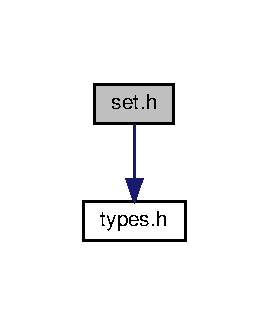
\includegraphics[width=129pt]{set_8h__incl}
\end{center}
\end{figure}
This graph shows which files directly or indirectly include this file\+:
\nopagebreak
\begin{figure}[H]
\begin{center}
\leavevmode
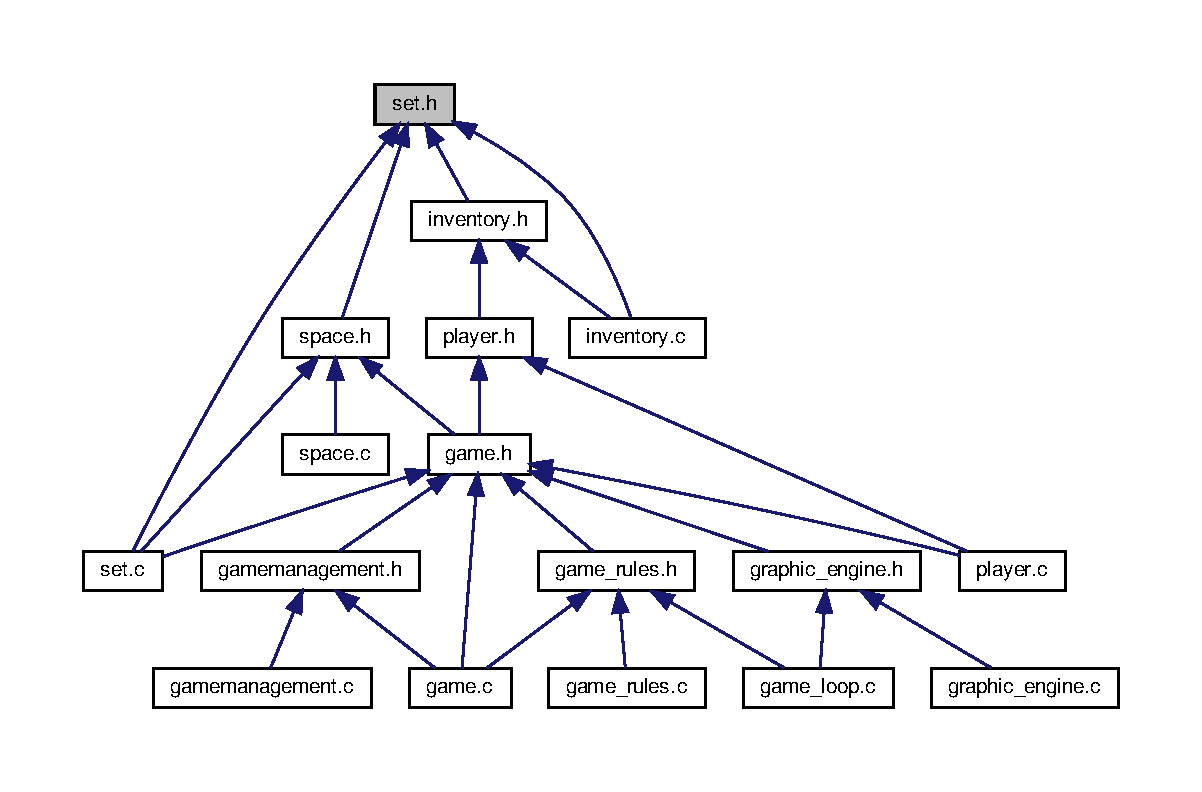
\includegraphics[width=350pt]{set_8h__dep__incl}
\end{center}
\end{figure}
\subsection*{Macros}
\begin{DoxyCompactItemize}
\item 
\mbox{\Hypertarget{set_8h_a0ffebf572977a670aba207757c157eba}\label{set_8h_a0ffebf572977a670aba207757c157eba}} 
\#define \hyperlink{set_8h_a0ffebf572977a670aba207757c157eba}{M\+A\+X\+\_\+\+I\+Ds\+\_\+\+S\+ET}~4
\begin{DoxyCompactList}\small\item\em defines max number of ids \end{DoxyCompactList}\end{DoxyCompactItemize}
\subsection*{Typedefs}
\begin{DoxyCompactItemize}
\item 
\mbox{\Hypertarget{set_8h_a6d3b7f7c92cbb4577ef3ef7ddbf93161}\label{set_8h_a6d3b7f7c92cbb4577ef3ef7ddbf93161}} 
typedef struct \hyperlink{struct__Set}{\+\_\+\+Set} \hyperlink{set_8h_a6d3b7f7c92cbb4577ef3ef7ddbf93161}{Set}
\begin{DoxyCompactList}\small\item\em defines structure of set \end{DoxyCompactList}\end{DoxyCompactItemize}
\subsection*{Functions}
\begin{DoxyCompactItemize}
\item 
\hyperlink{set_8h_a6d3b7f7c92cbb4577ef3ef7ddbf93161}{Set} $\ast$ \hyperlink{set_8h_abcc73b7ad3913fc92dd95d366c9c8687}{set\+\_\+create} ()
\begin{DoxyCompactList}\small\item\em create the set in the game \end{DoxyCompactList}\item 
\hyperlink{types_8h_a32c27cc471df37f4fc818d65de0a56c4}{S\+T\+A\+T\+US} \hyperlink{set_8h_a1f3a3f5d74c6dd9e9be0ec515fae282a}{set\+\_\+destroy} (\hyperlink{set_8h_a6d3b7f7c92cbb4577ef3ef7ddbf93161}{Set} $\ast$aux)
\begin{DoxyCompactList}\small\item\em destroy the set in the game \end{DoxyCompactList}\item 
\hyperlink{types_8h_a3e5b8192e7d9ffaf3542f1210aec18dd}{B\+O\+OL} \hyperlink{set_8h_a6426d210af9f56c938fba5f221ec6a80}{set\+\_\+id\+\_\+in} (\hyperlink{set_8h_a6d3b7f7c92cbb4577ef3ef7ddbf93161}{Set} $\ast$aux, \hyperlink{types_8h_a845e604fb28f7e3d97549da3448149d3}{Id} var)
\begin{DoxyCompactList}\small\item\em set the id in the game \end{DoxyCompactList}\item 
\hyperlink{types_8h_a32c27cc471df37f4fc818d65de0a56c4}{S\+T\+A\+T\+US} \hyperlink{set_8h_ab43446d7f625f4b646da3810609ef92d}{set\+\_\+id\+\_\+add} (\hyperlink{set_8h_a6d3b7f7c92cbb4577ef3ef7ddbf93161}{Set} $\ast$aux, \hyperlink{types_8h_a845e604fb28f7e3d97549da3448149d3}{Id} new)
\begin{DoxyCompactList}\small\item\em set the id add in the game \end{DoxyCompactList}\item 
\hyperlink{types_8h_a32c27cc471df37f4fc818d65de0a56c4}{S\+T\+A\+T\+US} \hyperlink{set_8h_a7c68c583fc56840769f93dd8a0e24d8a}{set\+\_\+remov\+\_\+id} (\hyperlink{set_8h_a6d3b7f7c92cbb4577ef3ef7ddbf93161}{Set} $\ast$aux, \hyperlink{types_8h_a845e604fb28f7e3d97549da3448149d3}{Id} rmv)
\begin{DoxyCompactList}\small\item\em remove the id add in the game \end{DoxyCompactList}\item 
\hyperlink{types_8h_a845e604fb28f7e3d97549da3448149d3}{Id} \hyperlink{set_8h_a68b44d04ca0d7ba5b3e949f04dd2f8ff}{set\+\_\+get\+\_\+id} (\hyperlink{set_8h_a6d3b7f7c92cbb4577ef3ef7ddbf93161}{Set} $\ast$aux, int pos)
\begin{DoxyCompactList}\small\item\em set the id add in the game \end{DoxyCompactList}\item 
\hyperlink{types_8h_a32c27cc471df37f4fc818d65de0a56c4}{S\+T\+A\+T\+US} \hyperlink{set_8h_afb5717fc0d782e62066cfe40960d5362}{set\+\_\+set\+\_\+id} (\hyperlink{set_8h_a6d3b7f7c92cbb4577ef3ef7ddbf93161}{Set} $\ast$aux, \hyperlink{types_8h_a845e604fb28f7e3d97549da3448149d3}{Id} id, int pos)
\begin{DoxyCompactList}\small\item\em set the id in the game \end{DoxyCompactList}\item 
int \hyperlink{set_8h_a69784555363e44d97c4f6c0119bc52d8}{set\+\_\+get\+Num} (\hyperlink{set_8h_a6d3b7f7c92cbb4577ef3ef7ddbf93161}{Set} $\ast$set)
\begin{DoxyCompactList}\small\item\em set get number in the game \end{DoxyCompactList}\item 
\hyperlink{types_8h_a32c27cc471df37f4fc818d65de0a56c4}{S\+T\+A\+T\+US} \hyperlink{set_8h_a38ab539c50ee57aae502ee63657bcf22}{set\+\_\+print} (\hyperlink{set_8h_a6d3b7f7c92cbb4577ef3ef7ddbf93161}{Set} $\ast$aux)
\begin{DoxyCompactList}\small\item\em prints the set \end{DoxyCompactList}\end{DoxyCompactItemize}


\subsection{Detailed Description}
It defines the header of set. 

\begin{DoxyAuthor}{Author}
\end{DoxyAuthor}
\begin{DoxyVersion}{Version}
2.\+0 
\end{DoxyVersion}
\begin{DoxyDate}{Date}
21-\/02-\/2019 
\end{DoxyDate}
\begin{DoxyCopyright}{Copyright}
G\+NU Public License 
\end{DoxyCopyright}


\subsection{Function Documentation}
\mbox{\Hypertarget{set_8h_abcc73b7ad3913fc92dd95d366c9c8687}\label{set_8h_abcc73b7ad3913fc92dd95d366c9c8687}} 
\index{set.\+h@{set.\+h}!set\+\_\+create@{set\+\_\+create}}
\index{set\+\_\+create@{set\+\_\+create}!set.\+h@{set.\+h}}
\subsubsection{\texorpdfstring{set\+\_\+create()}{set\_create()}}
{\footnotesize\ttfamily \hyperlink{set_8h_a6d3b7f7c92cbb4577ef3ef7ddbf93161}{Set}$\ast$ set\+\_\+create (\begin{DoxyParamCaption}{ }\end{DoxyParamCaption})}



create the set in the game 

\begin{DoxyReturn}{Returns}
set or in case of error N\+U\+LL 
\end{DoxyReturn}
\mbox{\Hypertarget{set_8h_a1f3a3f5d74c6dd9e9be0ec515fae282a}\label{set_8h_a1f3a3f5d74c6dd9e9be0ec515fae282a}} 
\index{set.\+h@{set.\+h}!set\+\_\+destroy@{set\+\_\+destroy}}
\index{set\+\_\+destroy@{set\+\_\+destroy}!set.\+h@{set.\+h}}
\subsubsection{\texorpdfstring{set\+\_\+destroy()}{set\_destroy()}}
{\footnotesize\ttfamily \hyperlink{types_8h_a32c27cc471df37f4fc818d65de0a56c4}{S\+T\+A\+T\+US} set\+\_\+destroy (\begin{DoxyParamCaption}\item[{\hyperlink{set_8h_a6d3b7f7c92cbb4577ef3ef7ddbf93161}{Set} $\ast$}]{aux }\end{DoxyParamCaption})}



destroy the set in the game 


\begin{DoxyParams}{Parameters}
{\em aux} & \\
\hline
\end{DoxyParams}
\begin{DoxyReturn}{Returns}
OK, or E\+R\+R\+OR 
\end{DoxyReturn}
\mbox{\Hypertarget{set_8h_a68b44d04ca0d7ba5b3e949f04dd2f8ff}\label{set_8h_a68b44d04ca0d7ba5b3e949f04dd2f8ff}} 
\index{set.\+h@{set.\+h}!set\+\_\+get\+\_\+id@{set\+\_\+get\+\_\+id}}
\index{set\+\_\+get\+\_\+id@{set\+\_\+get\+\_\+id}!set.\+h@{set.\+h}}
\subsubsection{\texorpdfstring{set\+\_\+get\+\_\+id()}{set\_get\_id()}}
{\footnotesize\ttfamily \hyperlink{types_8h_a845e604fb28f7e3d97549da3448149d3}{Id} set\+\_\+get\+\_\+id (\begin{DoxyParamCaption}\item[{\hyperlink{set_8h_a6d3b7f7c92cbb4577ef3ef7ddbf93161}{Set} $\ast$}]{aux,  }\item[{int}]{pos }\end{DoxyParamCaption})}



set the id add in the game 


\begin{DoxyParams}{Parameters}
{\em aux} & \\
\hline
{\em pos} & \\
\hline
\end{DoxyParams}
\begin{DoxyReturn}{Returns}
id or in case of error N\+U\+LL 
\end{DoxyReturn}
\mbox{\Hypertarget{set_8h_a69784555363e44d97c4f6c0119bc52d8}\label{set_8h_a69784555363e44d97c4f6c0119bc52d8}} 
\index{set.\+h@{set.\+h}!set\+\_\+get\+Num@{set\+\_\+get\+Num}}
\index{set\+\_\+get\+Num@{set\+\_\+get\+Num}!set.\+h@{set.\+h}}
\subsubsection{\texorpdfstring{set\+\_\+get\+Num()}{set\_getNum()}}
{\footnotesize\ttfamily int set\+\_\+get\+Num (\begin{DoxyParamCaption}\item[{\hyperlink{set_8h_a6d3b7f7c92cbb4577ef3ef7ddbf93161}{Set} $\ast$}]{set }\end{DoxyParamCaption})}



set get number in the game 


\begin{DoxyParams}{Parameters}
{\em set} & \\
\hline
\end{DoxyParams}
\begin{DoxyReturn}{Returns}
number of sets 
\end{DoxyReturn}
\mbox{\Hypertarget{set_8h_ab43446d7f625f4b646da3810609ef92d}\label{set_8h_ab43446d7f625f4b646da3810609ef92d}} 
\index{set.\+h@{set.\+h}!set\+\_\+id\+\_\+add@{set\+\_\+id\+\_\+add}}
\index{set\+\_\+id\+\_\+add@{set\+\_\+id\+\_\+add}!set.\+h@{set.\+h}}
\subsubsection{\texorpdfstring{set\+\_\+id\+\_\+add()}{set\_id\_add()}}
{\footnotesize\ttfamily \hyperlink{types_8h_a32c27cc471df37f4fc818d65de0a56c4}{S\+T\+A\+T\+US} set\+\_\+id\+\_\+add (\begin{DoxyParamCaption}\item[{\hyperlink{set_8h_a6d3b7f7c92cbb4577ef3ef7ddbf93161}{Set} $\ast$}]{aux,  }\item[{\hyperlink{types_8h_a845e604fb28f7e3d97549da3448149d3}{Id}}]{new }\end{DoxyParamCaption})}



set the id add in the game 


\begin{DoxyParams}{Parameters}
{\em aux} & \\
\hline
{\em new} & \\
\hline
\end{DoxyParams}
\begin{DoxyReturn}{Returns}
OK, or E\+R\+R\+OR 
\end{DoxyReturn}
\mbox{\Hypertarget{set_8h_a6426d210af9f56c938fba5f221ec6a80}\label{set_8h_a6426d210af9f56c938fba5f221ec6a80}} 
\index{set.\+h@{set.\+h}!set\+\_\+id\+\_\+in@{set\+\_\+id\+\_\+in}}
\index{set\+\_\+id\+\_\+in@{set\+\_\+id\+\_\+in}!set.\+h@{set.\+h}}
\subsubsection{\texorpdfstring{set\+\_\+id\+\_\+in()}{set\_id\_in()}}
{\footnotesize\ttfamily \hyperlink{types_8h_a3e5b8192e7d9ffaf3542f1210aec18dd}{B\+O\+OL} set\+\_\+id\+\_\+in (\begin{DoxyParamCaption}\item[{\hyperlink{set_8h_a6d3b7f7c92cbb4577ef3ef7ddbf93161}{Set} $\ast$}]{aux,  }\item[{\hyperlink{types_8h_a845e604fb28f7e3d97549da3448149d3}{Id}}]{var }\end{DoxyParamCaption})}



set the id in the game 


\begin{DoxyParams}{Parameters}
{\em aux} & \\
\hline
{\em var} & \\
\hline
\end{DoxyParams}
\begin{DoxyReturn}{Returns}
T\+R\+UE or F\+A\+L\+SE 
\end{DoxyReturn}
\mbox{\Hypertarget{set_8h_a38ab539c50ee57aae502ee63657bcf22}\label{set_8h_a38ab539c50ee57aae502ee63657bcf22}} 
\index{set.\+h@{set.\+h}!set\+\_\+print@{set\+\_\+print}}
\index{set\+\_\+print@{set\+\_\+print}!set.\+h@{set.\+h}}
\subsubsection{\texorpdfstring{set\+\_\+print()}{set\_print()}}
{\footnotesize\ttfamily \hyperlink{types_8h_a32c27cc471df37f4fc818d65de0a56c4}{S\+T\+A\+T\+US} set\+\_\+print (\begin{DoxyParamCaption}\item[{\hyperlink{set_8h_a6d3b7f7c92cbb4577ef3ef7ddbf93161}{Set} $\ast$}]{aux }\end{DoxyParamCaption})}



prints the set 


\begin{DoxyParams}{Parameters}
{\em aux} & \\
\hline
\end{DoxyParams}
\begin{DoxyReturn}{Returns}
OK, or E\+R\+R\+OR 
\end{DoxyReturn}
\mbox{\Hypertarget{set_8h_a7c68c583fc56840769f93dd8a0e24d8a}\label{set_8h_a7c68c583fc56840769f93dd8a0e24d8a}} 
\index{set.\+h@{set.\+h}!set\+\_\+remov\+\_\+id@{set\+\_\+remov\+\_\+id}}
\index{set\+\_\+remov\+\_\+id@{set\+\_\+remov\+\_\+id}!set.\+h@{set.\+h}}
\subsubsection{\texorpdfstring{set\+\_\+remov\+\_\+id()}{set\_remov\_id()}}
{\footnotesize\ttfamily \hyperlink{types_8h_a32c27cc471df37f4fc818d65de0a56c4}{S\+T\+A\+T\+US} set\+\_\+remov\+\_\+id (\begin{DoxyParamCaption}\item[{\hyperlink{set_8h_a6d3b7f7c92cbb4577ef3ef7ddbf93161}{Set} $\ast$}]{aux,  }\item[{\hyperlink{types_8h_a845e604fb28f7e3d97549da3448149d3}{Id}}]{rmv }\end{DoxyParamCaption})}



remove the id add in the game 


\begin{DoxyParams}{Parameters}
{\em aux} & \\
\hline
{\em rmv} & \\
\hline
\end{DoxyParams}
\begin{DoxyReturn}{Returns}
OK, or E\+R\+R\+OR 
\end{DoxyReturn}
\mbox{\Hypertarget{set_8h_afb5717fc0d782e62066cfe40960d5362}\label{set_8h_afb5717fc0d782e62066cfe40960d5362}} 
\index{set.\+h@{set.\+h}!set\+\_\+set\+\_\+id@{set\+\_\+set\+\_\+id}}
\index{set\+\_\+set\+\_\+id@{set\+\_\+set\+\_\+id}!set.\+h@{set.\+h}}
\subsubsection{\texorpdfstring{set\+\_\+set\+\_\+id()}{set\_set\_id()}}
{\footnotesize\ttfamily \hyperlink{types_8h_a32c27cc471df37f4fc818d65de0a56c4}{S\+T\+A\+T\+US} set\+\_\+set\+\_\+id (\begin{DoxyParamCaption}\item[{\hyperlink{set_8h_a6d3b7f7c92cbb4577ef3ef7ddbf93161}{Set} $\ast$}]{aux,  }\item[{\hyperlink{types_8h_a845e604fb28f7e3d97549da3448149d3}{Id}}]{id,  }\item[{int}]{pos }\end{DoxyParamCaption})}



set the id in the game 


\begin{DoxyParams}{Parameters}
{\em aux} & \\
\hline
{\em pos} & \\
\hline
{\em id} & \\
\hline
\end{DoxyParams}
\begin{DoxyReturn}{Returns}
OK, or E\+R\+R\+OR 
\end{DoxyReturn}


\hypertarget{space_8c}{}\section{space.\+c File Reference}
\label{space_8c}\index{space.\+c@{space.\+c}}


It defines the module of space.  


{\ttfamily \#include $<$stdio.\+h$>$}\newline
{\ttfamily \#include $<$stdlib.\+h$>$}\newline
{\ttfamily \#include $<$string.\+h$>$}\newline
{\ttfamily \#include \char`\"{}types.\+h\char`\"{}}\newline
{\ttfamily \#include \char`\"{}space.\+h\char`\"{}}\newline
Include dependency graph for space.\+c\+:
\nopagebreak
\begin{figure}[H]
\begin{center}
\leavevmode
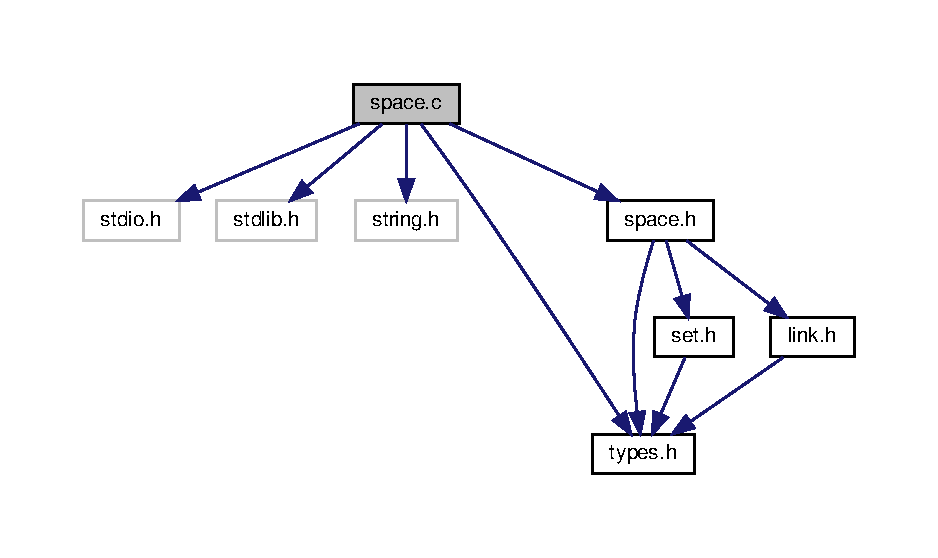
\includegraphics[width=350pt]{space_8c__incl}
\end{center}
\end{figure}
\subsection*{Data Structures}
\begin{DoxyCompactItemize}
\item 
struct \hyperlink{struct__Space}{\+\_\+\+Space}
\begin{DoxyCompactList}\small\item\em defines the structure of space \end{DoxyCompactList}\end{DoxyCompactItemize}
\subsection*{Functions}
\begin{DoxyCompactItemize}
\item 
\hyperlink{space_8h_a67533ffc2b70463baecc38fb0629bbfc}{Space} $\ast$ \hyperlink{space_8c_a162866fcea156b800fd546d0ffd271c9}{space\+\_\+create} (\hyperlink{types_8h_a845e604fb28f7e3d97549da3448149d3}{Id} id)
\begin{DoxyCompactList}\small\item\em create the space in the game \end{DoxyCompactList}\item 
\hyperlink{types_8h_a32c27cc471df37f4fc818d65de0a56c4}{S\+T\+A\+T\+US} \hyperlink{space_8c_a5c70c70398923693ddbe4dfac8d72a0d}{space\+\_\+destroy} (\hyperlink{space_8h_a67533ffc2b70463baecc38fb0629bbfc}{Space} $\ast$space)
\begin{DoxyCompactList}\small\item\em destroy the space in the game \end{DoxyCompactList}\item 
\hyperlink{types_8h_a32c27cc471df37f4fc818d65de0a56c4}{S\+T\+A\+T\+US} \hyperlink{space_8c_aab5b468f9822ab78dbe16d1321870d93}{space\+\_\+set\+\_\+name} (\hyperlink{space_8h_a67533ffc2b70463baecc38fb0629bbfc}{Space} $\ast$space, char $\ast$name)
\begin{DoxyCompactList}\small\item\em set the id of space \end{DoxyCompactList}\item 
\hyperlink{types_8h_a32c27cc471df37f4fc818d65de0a56c4}{S\+T\+A\+T\+US} \hyperlink{space_8c_ac69528ddf930a534d57c5d1d74691f1d}{space\+\_\+set\+\_\+description} (\hyperlink{space_8h_a67533ffc2b70463baecc38fb0629bbfc}{Space} $\ast$space, char $\ast$desc)
\begin{DoxyCompactList}\small\item\em set the descripcion of objects \end{DoxyCompactList}\item 
\hyperlink{types_8h_a32c27cc471df37f4fc818d65de0a56c4}{S\+T\+A\+T\+US} \hyperlink{space_8c_a9e6e3e3bac4996ac6b8bd555e52bfb26}{space\+\_\+set\+\_\+north} (\hyperlink{space_8h_a67533ffc2b70463baecc38fb0629bbfc}{Space} $\ast$space, \hyperlink{types_8h_a845e604fb28f7e3d97549da3448149d3}{Id} id)
\begin{DoxyCompactList}\small\item\em set the north id of space \end{DoxyCompactList}\item 
\hyperlink{types_8h_a32c27cc471df37f4fc818d65de0a56c4}{S\+T\+A\+T\+US} \hyperlink{space_8c_a422ab9f220b4c471c44256a27377de1a}{space\+\_\+set\+\_\+south} (\hyperlink{space_8h_a67533ffc2b70463baecc38fb0629bbfc}{Space} $\ast$space, \hyperlink{types_8h_a845e604fb28f7e3d97549da3448149d3}{Id} id)
\begin{DoxyCompactList}\small\item\em set the south id of space \end{DoxyCompactList}\item 
\hyperlink{types_8h_a32c27cc471df37f4fc818d65de0a56c4}{S\+T\+A\+T\+US} \hyperlink{space_8c_a860a8f3e0227955ad56d1a12f0bdc44a}{space\+\_\+set\+\_\+east} (\hyperlink{space_8h_a67533ffc2b70463baecc38fb0629bbfc}{Space} $\ast$space, \hyperlink{types_8h_a845e604fb28f7e3d97549da3448149d3}{Id} id)
\begin{DoxyCompactList}\small\item\em set the east id of space \end{DoxyCompactList}\item 
\hyperlink{types_8h_a32c27cc471df37f4fc818d65de0a56c4}{S\+T\+A\+T\+US} \hyperlink{space_8c_ad44b14cb38902cf31fa1f341beaab0db}{space\+\_\+set\+\_\+west} (\hyperlink{space_8h_a67533ffc2b70463baecc38fb0629bbfc}{Space} $\ast$space, \hyperlink{types_8h_a845e604fb28f7e3d97549da3448149d3}{Id} id)
\begin{DoxyCompactList}\small\item\em set the west id of space \end{DoxyCompactList}\item 
\hyperlink{types_8h_a32c27cc471df37f4fc818d65de0a56c4}{S\+T\+A\+T\+US} \hyperlink{space_8c_a510c703a1eeac8965932394a900a43cc}{space\+\_\+set\+\_\+object} (\hyperlink{space_8h_a67533ffc2b70463baecc38fb0629bbfc}{Space} $\ast$space, \hyperlink{types_8h_a845e604fb28f7e3d97549da3448149d3}{Id} value)
\begin{DoxyCompactList}\small\item\em set the object to the space \end{DoxyCompactList}\item 
const char $\ast$ \hyperlink{space_8c_a51e854a2f9b35bd39e60c04ec5f03abd}{space\+\_\+get\+\_\+description} (\hyperlink{space_8h_a67533ffc2b70463baecc38fb0629bbfc}{Space} $\ast$space)
\begin{DoxyCompactList}\small\item\em get the descripcion of objects \end{DoxyCompactList}\item 
const char $\ast$ \hyperlink{space_8c_a310c540cd6e11073f7328add1f927001}{space\+\_\+get\+\_\+name} (\hyperlink{space_8h_a67533ffc2b70463baecc38fb0629bbfc}{Space} $\ast$space)
\begin{DoxyCompactList}\small\item\em get the name of space \end{DoxyCompactList}\item 
\hyperlink{types_8h_a845e604fb28f7e3d97549da3448149d3}{Id} \hyperlink{space_8c_ac8ddfd0d8692fd852ee49698c446cb50}{space\+\_\+get\+\_\+id} (\hyperlink{space_8h_a67533ffc2b70463baecc38fb0629bbfc}{Space} $\ast$space)
\begin{DoxyCompactList}\small\item\em get the id of space \end{DoxyCompactList}\item 
\hyperlink{types_8h_a845e604fb28f7e3d97549da3448149d3}{Id} \hyperlink{space_8c_ad331fba774897900f615d9d2e8d81a90}{space\+\_\+get\+\_\+north} (\hyperlink{space_8h_a67533ffc2b70463baecc38fb0629bbfc}{Space} $\ast$space)
\begin{DoxyCompactList}\small\item\em get the north id of space \end{DoxyCompactList}\item 
\hyperlink{types_8h_a845e604fb28f7e3d97549da3448149d3}{Id} \hyperlink{space_8c_a9b86e1335c423eaad832e50d4c12cf1f}{space\+\_\+get\+\_\+south} (\hyperlink{space_8h_a67533ffc2b70463baecc38fb0629bbfc}{Space} $\ast$space)
\begin{DoxyCompactList}\small\item\em get the south id of space \end{DoxyCompactList}\item 
\hyperlink{types_8h_a845e604fb28f7e3d97549da3448149d3}{Id} \hyperlink{space_8c_a978a22b77f74bb2dab68a00571abbe0b}{space\+\_\+get\+\_\+east} (\hyperlink{space_8h_a67533ffc2b70463baecc38fb0629bbfc}{Space} $\ast$space)
\begin{DoxyCompactList}\small\item\em get the east id of space \end{DoxyCompactList}\item 
\hyperlink{types_8h_a845e604fb28f7e3d97549da3448149d3}{Id} \hyperlink{space_8c_af495ebfd5d13eba1a48cebd10992a17f}{space\+\_\+get\+\_\+west} (\hyperlink{space_8h_a67533ffc2b70463baecc38fb0629bbfc}{Space} $\ast$space)
\begin{DoxyCompactList}\small\item\em get the west id of space \end{DoxyCompactList}\item 
\hyperlink{set_8h_a6d3b7f7c92cbb4577ef3ef7ddbf93161}{Set} $\ast$ \hyperlink{space_8c_ab24abae4e127bf0bca596cd71ba3aad6}{space\+\_\+get\+\_\+object} (\hyperlink{space_8h_a67533ffc2b70463baecc38fb0629bbfc}{Space} $\ast$space)
\begin{DoxyCompactList}\small\item\em get the object to the space \end{DoxyCompactList}\item 
\hyperlink{types_8h_a32c27cc471df37f4fc818d65de0a56c4}{S\+T\+A\+T\+US} \hyperlink{space_8c_a18eca058da6cdf20ae5eda9d122d992e}{space\+\_\+print} (\hyperlink{space_8h_a67533ffc2b70463baecc38fb0629bbfc}{Space} $\ast$space)
\begin{DoxyCompactList}\small\item\em print the object of the space \end{DoxyCompactList}\item 
char $\ast$ \hyperlink{space_8c_abc33179385bc05971038bf0eb68b2d3a}{space\+\_\+get\+\_\+gdesc} (\hyperlink{space_8h_a67533ffc2b70463baecc38fb0629bbfc}{Space} $\ast$space, int i)
\begin{DoxyCompactList}\small\item\em get the objec gdesc \end{DoxyCompactList}\item 
char $\ast$ \hyperlink{space_8c_ae8a9b9294e8b285d680d3ce2c470f4b9}{space\+\_\+create\+\_\+gdesc} ()
\begin{DoxyCompactList}\small\item\em set the objec gdesc \end{DoxyCompactList}\item 
\hyperlink{types_8h_a32c27cc471df37f4fc818d65de0a56c4}{S\+T\+A\+T\+US} \hyperlink{space_8c_a3723b291fc3cbbd723622ee0f9b52a62}{space\+\_\+set\+\_\+gdesc} (\hyperlink{space_8h_a67533ffc2b70463baecc38fb0629bbfc}{Space} $\ast$space, char $\ast$str, int i)
\begin{DoxyCompactList}\small\item\em set the objec gdesc to space \end{DoxyCompactList}\end{DoxyCompactItemize}


\subsection{Detailed Description}
It defines the module of space. 

\begin{DoxyAuthor}{Author}
\end{DoxyAuthor}
\begin{DoxyVersion}{Version}
2.\+0 
\end{DoxyVersion}
\begin{DoxyDate}{Date}
04-\/02-\/2019 
\end{DoxyDate}
\begin{DoxyCopyright}{Copyright}
G\+NU Public License 
\end{DoxyCopyright}


\subsection{Function Documentation}
\mbox{\Hypertarget{space_8c_a162866fcea156b800fd546d0ffd271c9}\label{space_8c_a162866fcea156b800fd546d0ffd271c9}} 
\index{space.\+c@{space.\+c}!space\+\_\+create@{space\+\_\+create}}
\index{space\+\_\+create@{space\+\_\+create}!space.\+c@{space.\+c}}
\subsubsection{\texorpdfstring{space\+\_\+create()}{space\_create()}}
{\footnotesize\ttfamily \hyperlink{space_8h_a67533ffc2b70463baecc38fb0629bbfc}{Space}$\ast$ space\+\_\+create (\begin{DoxyParamCaption}\item[{\hyperlink{types_8h_a845e604fb28f7e3d97549da3448149d3}{Id}}]{id }\end{DoxyParamCaption})}



create the space in the game 


\begin{DoxyParams}{Parameters}
{\em id} & \\
\hline
\end{DoxyParams}
\begin{DoxyReturn}{Returns}
space or in case of error N\+U\+LL 
\end{DoxyReturn}
\mbox{\Hypertarget{space_8c_ae8a9b9294e8b285d680d3ce2c470f4b9}\label{space_8c_ae8a9b9294e8b285d680d3ce2c470f4b9}} 
\index{space.\+c@{space.\+c}!space\+\_\+create\+\_\+gdesc@{space\+\_\+create\+\_\+gdesc}}
\index{space\+\_\+create\+\_\+gdesc@{space\+\_\+create\+\_\+gdesc}!space.\+c@{space.\+c}}
\subsubsection{\texorpdfstring{space\+\_\+create\+\_\+gdesc()}{space\_create\_gdesc()}}
{\footnotesize\ttfamily char$\ast$ space\+\_\+create\+\_\+gdesc (\begin{DoxyParamCaption}{ }\end{DoxyParamCaption})}



set the objec gdesc 

\begin{DoxyReturn}{Returns}
char or in case of error N\+U\+LL 
\end{DoxyReturn}
\mbox{\Hypertarget{space_8c_a5c70c70398923693ddbe4dfac8d72a0d}\label{space_8c_a5c70c70398923693ddbe4dfac8d72a0d}} 
\index{space.\+c@{space.\+c}!space\+\_\+destroy@{space\+\_\+destroy}}
\index{space\+\_\+destroy@{space\+\_\+destroy}!space.\+c@{space.\+c}}
\subsubsection{\texorpdfstring{space\+\_\+destroy()}{space\_destroy()}}
{\footnotesize\ttfamily \hyperlink{types_8h_a32c27cc471df37f4fc818d65de0a56c4}{S\+T\+A\+T\+US} space\+\_\+destroy (\begin{DoxyParamCaption}\item[{\hyperlink{space_8h_a67533ffc2b70463baecc38fb0629bbfc}{Space} $\ast$}]{space }\end{DoxyParamCaption})}



destroy the space in the game 


\begin{DoxyParams}{Parameters}
{\em space} & \\
\hline
\end{DoxyParams}
\begin{DoxyReturn}{Returns}
OK, or E\+R\+R\+OR 
\end{DoxyReturn}
\mbox{\Hypertarget{space_8c_a51e854a2f9b35bd39e60c04ec5f03abd}\label{space_8c_a51e854a2f9b35bd39e60c04ec5f03abd}} 
\index{space.\+c@{space.\+c}!space\+\_\+get\+\_\+description@{space\+\_\+get\+\_\+description}}
\index{space\+\_\+get\+\_\+description@{space\+\_\+get\+\_\+description}!space.\+c@{space.\+c}}
\subsubsection{\texorpdfstring{space\+\_\+get\+\_\+description()}{space\_get\_description()}}
{\footnotesize\ttfamily const char$\ast$ space\+\_\+get\+\_\+description (\begin{DoxyParamCaption}\item[{\hyperlink{space_8h_a67533ffc2b70463baecc38fb0629bbfc}{Space} $\ast$}]{space }\end{DoxyParamCaption})}



get the descripcion of objects 


\begin{DoxyParams}{Parameters}
{\em space} & \\
\hline
\end{DoxyParams}
\begin{DoxyReturn}{Returns}
char or in case of error N\+U\+LL 
\end{DoxyReturn}
\mbox{\Hypertarget{space_8c_a978a22b77f74bb2dab68a00571abbe0b}\label{space_8c_a978a22b77f74bb2dab68a00571abbe0b}} 
\index{space.\+c@{space.\+c}!space\+\_\+get\+\_\+east@{space\+\_\+get\+\_\+east}}
\index{space\+\_\+get\+\_\+east@{space\+\_\+get\+\_\+east}!space.\+c@{space.\+c}}
\subsubsection{\texorpdfstring{space\+\_\+get\+\_\+east()}{space\_get\_east()}}
{\footnotesize\ttfamily \hyperlink{types_8h_a845e604fb28f7e3d97549da3448149d3}{Id} space\+\_\+get\+\_\+east (\begin{DoxyParamCaption}\item[{\hyperlink{space_8h_a67533ffc2b70463baecc38fb0629bbfc}{Space} $\ast$}]{space }\end{DoxyParamCaption})}



get the east id of space 


\begin{DoxyParams}{Parameters}
{\em space} & \\
\hline
\end{DoxyParams}
\begin{DoxyReturn}{Returns}
id or in case of error N\+U\+LL 
\end{DoxyReturn}
\mbox{\Hypertarget{space_8c_abc33179385bc05971038bf0eb68b2d3a}\label{space_8c_abc33179385bc05971038bf0eb68b2d3a}} 
\index{space.\+c@{space.\+c}!space\+\_\+get\+\_\+gdesc@{space\+\_\+get\+\_\+gdesc}}
\index{space\+\_\+get\+\_\+gdesc@{space\+\_\+get\+\_\+gdesc}!space.\+c@{space.\+c}}
\subsubsection{\texorpdfstring{space\+\_\+get\+\_\+gdesc()}{space\_get\_gdesc()}}
{\footnotesize\ttfamily char$\ast$ space\+\_\+get\+\_\+gdesc (\begin{DoxyParamCaption}\item[{\hyperlink{space_8h_a67533ffc2b70463baecc38fb0629bbfc}{Space} $\ast$}]{space,  }\item[{int}]{i }\end{DoxyParamCaption})}



get the objec gdesc 


\begin{DoxyParams}{Parameters}
{\em space} & \\
\hline
{\em i} & \\
\hline
\end{DoxyParams}
\begin{DoxyReturn}{Returns}
char or in case of error N\+U\+LL 
\end{DoxyReturn}
\mbox{\Hypertarget{space_8c_ac8ddfd0d8692fd852ee49698c446cb50}\label{space_8c_ac8ddfd0d8692fd852ee49698c446cb50}} 
\index{space.\+c@{space.\+c}!space\+\_\+get\+\_\+id@{space\+\_\+get\+\_\+id}}
\index{space\+\_\+get\+\_\+id@{space\+\_\+get\+\_\+id}!space.\+c@{space.\+c}}
\subsubsection{\texorpdfstring{space\+\_\+get\+\_\+id()}{space\_get\_id()}}
{\footnotesize\ttfamily \hyperlink{types_8h_a845e604fb28f7e3d97549da3448149d3}{Id} space\+\_\+get\+\_\+id (\begin{DoxyParamCaption}\item[{\hyperlink{space_8h_a67533ffc2b70463baecc38fb0629bbfc}{Space} $\ast$}]{space }\end{DoxyParamCaption})}



get the id of space 


\begin{DoxyParams}{Parameters}
{\em space} & \\
\hline
\end{DoxyParams}
\begin{DoxyReturn}{Returns}
id or in case of error N\+U\+LL 
\end{DoxyReturn}
\mbox{\Hypertarget{space_8c_a310c540cd6e11073f7328add1f927001}\label{space_8c_a310c540cd6e11073f7328add1f927001}} 
\index{space.\+c@{space.\+c}!space\+\_\+get\+\_\+name@{space\+\_\+get\+\_\+name}}
\index{space\+\_\+get\+\_\+name@{space\+\_\+get\+\_\+name}!space.\+c@{space.\+c}}
\subsubsection{\texorpdfstring{space\+\_\+get\+\_\+name()}{space\_get\_name()}}
{\footnotesize\ttfamily const char$\ast$ space\+\_\+get\+\_\+name (\begin{DoxyParamCaption}\item[{\hyperlink{space_8h_a67533ffc2b70463baecc38fb0629bbfc}{Space} $\ast$}]{space }\end{DoxyParamCaption})}



get the name of space 


\begin{DoxyParams}{Parameters}
{\em space} & \\
\hline
\end{DoxyParams}
\begin{DoxyReturn}{Returns}
name of space or in case of error N\+U\+LL 
\end{DoxyReturn}
\mbox{\Hypertarget{space_8c_ad331fba774897900f615d9d2e8d81a90}\label{space_8c_ad331fba774897900f615d9d2e8d81a90}} 
\index{space.\+c@{space.\+c}!space\+\_\+get\+\_\+north@{space\+\_\+get\+\_\+north}}
\index{space\+\_\+get\+\_\+north@{space\+\_\+get\+\_\+north}!space.\+c@{space.\+c}}
\subsubsection{\texorpdfstring{space\+\_\+get\+\_\+north()}{space\_get\_north()}}
{\footnotesize\ttfamily \hyperlink{types_8h_a845e604fb28f7e3d97549da3448149d3}{Id} space\+\_\+get\+\_\+north (\begin{DoxyParamCaption}\item[{\hyperlink{space_8h_a67533ffc2b70463baecc38fb0629bbfc}{Space} $\ast$}]{space }\end{DoxyParamCaption})}



get the north id of space 


\begin{DoxyParams}{Parameters}
{\em space} & \\
\hline
\end{DoxyParams}
\begin{DoxyReturn}{Returns}
id or in case of error N\+U\+LL 
\end{DoxyReturn}
\mbox{\Hypertarget{space_8c_ab24abae4e127bf0bca596cd71ba3aad6}\label{space_8c_ab24abae4e127bf0bca596cd71ba3aad6}} 
\index{space.\+c@{space.\+c}!space\+\_\+get\+\_\+object@{space\+\_\+get\+\_\+object}}
\index{space\+\_\+get\+\_\+object@{space\+\_\+get\+\_\+object}!space.\+c@{space.\+c}}
\subsubsection{\texorpdfstring{space\+\_\+get\+\_\+object()}{space\_get\_object()}}
{\footnotesize\ttfamily \hyperlink{set_8h_a6d3b7f7c92cbb4577ef3ef7ddbf93161}{Set}$\ast$ space\+\_\+get\+\_\+object (\begin{DoxyParamCaption}\item[{\hyperlink{space_8h_a67533ffc2b70463baecc38fb0629bbfc}{Space} $\ast$}]{space }\end{DoxyParamCaption})}



get the object to the space 


\begin{DoxyParams}{Parameters}
{\em space} & \\
\hline
\end{DoxyParams}
\begin{DoxyReturn}{Returns}
set or in case of error N\+U\+LL 
\end{DoxyReturn}
\mbox{\Hypertarget{space_8c_a9b86e1335c423eaad832e50d4c12cf1f}\label{space_8c_a9b86e1335c423eaad832e50d4c12cf1f}} 
\index{space.\+c@{space.\+c}!space\+\_\+get\+\_\+south@{space\+\_\+get\+\_\+south}}
\index{space\+\_\+get\+\_\+south@{space\+\_\+get\+\_\+south}!space.\+c@{space.\+c}}
\subsubsection{\texorpdfstring{space\+\_\+get\+\_\+south()}{space\_get\_south()}}
{\footnotesize\ttfamily \hyperlink{types_8h_a845e604fb28f7e3d97549da3448149d3}{Id} space\+\_\+get\+\_\+south (\begin{DoxyParamCaption}\item[{\hyperlink{space_8h_a67533ffc2b70463baecc38fb0629bbfc}{Space} $\ast$}]{space }\end{DoxyParamCaption})}



get the south id of space 


\begin{DoxyParams}{Parameters}
{\em space} & \\
\hline
\end{DoxyParams}
\begin{DoxyReturn}{Returns}
id or in case of error N\+U\+LL 
\end{DoxyReturn}
\mbox{\Hypertarget{space_8c_af495ebfd5d13eba1a48cebd10992a17f}\label{space_8c_af495ebfd5d13eba1a48cebd10992a17f}} 
\index{space.\+c@{space.\+c}!space\+\_\+get\+\_\+west@{space\+\_\+get\+\_\+west}}
\index{space\+\_\+get\+\_\+west@{space\+\_\+get\+\_\+west}!space.\+c@{space.\+c}}
\subsubsection{\texorpdfstring{space\+\_\+get\+\_\+west()}{space\_get\_west()}}
{\footnotesize\ttfamily \hyperlink{types_8h_a845e604fb28f7e3d97549da3448149d3}{Id} space\+\_\+get\+\_\+west (\begin{DoxyParamCaption}\item[{\hyperlink{space_8h_a67533ffc2b70463baecc38fb0629bbfc}{Space} $\ast$}]{space }\end{DoxyParamCaption})}



get the west id of space 


\begin{DoxyParams}{Parameters}
{\em space} & \\
\hline
\end{DoxyParams}
\begin{DoxyReturn}{Returns}
id or in case of error N\+U\+LL 
\end{DoxyReturn}
\mbox{\Hypertarget{space_8c_a18eca058da6cdf20ae5eda9d122d992e}\label{space_8c_a18eca058da6cdf20ae5eda9d122d992e}} 
\index{space.\+c@{space.\+c}!space\+\_\+print@{space\+\_\+print}}
\index{space\+\_\+print@{space\+\_\+print}!space.\+c@{space.\+c}}
\subsubsection{\texorpdfstring{space\+\_\+print()}{space\_print()}}
{\footnotesize\ttfamily \hyperlink{types_8h_a32c27cc471df37f4fc818d65de0a56c4}{S\+T\+A\+T\+US} space\+\_\+print (\begin{DoxyParamCaption}\item[{\hyperlink{space_8h_a67533ffc2b70463baecc38fb0629bbfc}{Space} $\ast$}]{space }\end{DoxyParamCaption})}



print the object of the space 


\begin{DoxyParams}{Parameters}
{\em space} & \\
\hline
\end{DoxyParams}
\begin{DoxyReturn}{Returns}
OK, or E\+R\+R\+OR 
\end{DoxyReturn}
\mbox{\Hypertarget{space_8c_ac69528ddf930a534d57c5d1d74691f1d}\label{space_8c_ac69528ddf930a534d57c5d1d74691f1d}} 
\index{space.\+c@{space.\+c}!space\+\_\+set\+\_\+description@{space\+\_\+set\+\_\+description}}
\index{space\+\_\+set\+\_\+description@{space\+\_\+set\+\_\+description}!space.\+c@{space.\+c}}
\subsubsection{\texorpdfstring{space\+\_\+set\+\_\+description()}{space\_set\_description()}}
{\footnotesize\ttfamily \hyperlink{types_8h_a32c27cc471df37f4fc818d65de0a56c4}{S\+T\+A\+T\+US} space\+\_\+set\+\_\+description (\begin{DoxyParamCaption}\item[{\hyperlink{space_8h_a67533ffc2b70463baecc38fb0629bbfc}{Space} $\ast$}]{space,  }\item[{char $\ast$}]{desc }\end{DoxyParamCaption})}



set the descripcion of objects 


\begin{DoxyParams}{Parameters}
{\em space} & \\
\hline
{\em desc} & \\
\hline
\end{DoxyParams}
\begin{DoxyReturn}{Returns}
OK, or E\+R\+R\+OR 
\end{DoxyReturn}
\mbox{\Hypertarget{space_8c_a860a8f3e0227955ad56d1a12f0bdc44a}\label{space_8c_a860a8f3e0227955ad56d1a12f0bdc44a}} 
\index{space.\+c@{space.\+c}!space\+\_\+set\+\_\+east@{space\+\_\+set\+\_\+east}}
\index{space\+\_\+set\+\_\+east@{space\+\_\+set\+\_\+east}!space.\+c@{space.\+c}}
\subsubsection{\texorpdfstring{space\+\_\+set\+\_\+east()}{space\_set\_east()}}
{\footnotesize\ttfamily \hyperlink{types_8h_a32c27cc471df37f4fc818d65de0a56c4}{S\+T\+A\+T\+US} space\+\_\+set\+\_\+east (\begin{DoxyParamCaption}\item[{\hyperlink{space_8h_a67533ffc2b70463baecc38fb0629bbfc}{Space} $\ast$}]{space,  }\item[{\hyperlink{types_8h_a845e604fb28f7e3d97549da3448149d3}{Id}}]{id }\end{DoxyParamCaption})}



set the east id of space 


\begin{DoxyParams}{Parameters}
{\em space} & \\
\hline
{\em id} & \\
\hline
\end{DoxyParams}
\begin{DoxyReturn}{Returns}
OK, or E\+R\+R\+OR 
\end{DoxyReturn}
\mbox{\Hypertarget{space_8c_a3723b291fc3cbbd723622ee0f9b52a62}\label{space_8c_a3723b291fc3cbbd723622ee0f9b52a62}} 
\index{space.\+c@{space.\+c}!space\+\_\+set\+\_\+gdesc@{space\+\_\+set\+\_\+gdesc}}
\index{space\+\_\+set\+\_\+gdesc@{space\+\_\+set\+\_\+gdesc}!space.\+c@{space.\+c}}
\subsubsection{\texorpdfstring{space\+\_\+set\+\_\+gdesc()}{space\_set\_gdesc()}}
{\footnotesize\ttfamily \hyperlink{types_8h_a32c27cc471df37f4fc818d65de0a56c4}{S\+T\+A\+T\+US} space\+\_\+set\+\_\+gdesc (\begin{DoxyParamCaption}\item[{\hyperlink{space_8h_a67533ffc2b70463baecc38fb0629bbfc}{Space} $\ast$}]{space,  }\item[{char $\ast$}]{str,  }\item[{int}]{i }\end{DoxyParamCaption})}



set the objec gdesc to space 


\begin{DoxyParams}{Parameters}
{\em space} & \\
\hline
{\em i} & \\
\hline
{\em str} & \\
\hline
\end{DoxyParams}
\begin{DoxyReturn}{Returns}
OK, or E\+R\+R\+OR 
\end{DoxyReturn}
\mbox{\Hypertarget{space_8c_aab5b468f9822ab78dbe16d1321870d93}\label{space_8c_aab5b468f9822ab78dbe16d1321870d93}} 
\index{space.\+c@{space.\+c}!space\+\_\+set\+\_\+name@{space\+\_\+set\+\_\+name}}
\index{space\+\_\+set\+\_\+name@{space\+\_\+set\+\_\+name}!space.\+c@{space.\+c}}
\subsubsection{\texorpdfstring{space\+\_\+set\+\_\+name()}{space\_set\_name()}}
{\footnotesize\ttfamily \hyperlink{types_8h_a32c27cc471df37f4fc818d65de0a56c4}{S\+T\+A\+T\+US} space\+\_\+set\+\_\+name (\begin{DoxyParamCaption}\item[{\hyperlink{space_8h_a67533ffc2b70463baecc38fb0629bbfc}{Space} $\ast$}]{space,  }\item[{char $\ast$}]{name }\end{DoxyParamCaption})}



set the id of space 


\begin{DoxyParams}{Parameters}
{\em space} & \\
\hline
{\em name} & \\
\hline
\end{DoxyParams}
\begin{DoxyReturn}{Returns}
OK, or E\+R\+R\+OR 
\end{DoxyReturn}
\mbox{\Hypertarget{space_8c_a9e6e3e3bac4996ac6b8bd555e52bfb26}\label{space_8c_a9e6e3e3bac4996ac6b8bd555e52bfb26}} 
\index{space.\+c@{space.\+c}!space\+\_\+set\+\_\+north@{space\+\_\+set\+\_\+north}}
\index{space\+\_\+set\+\_\+north@{space\+\_\+set\+\_\+north}!space.\+c@{space.\+c}}
\subsubsection{\texorpdfstring{space\+\_\+set\+\_\+north()}{space\_set\_north()}}
{\footnotesize\ttfamily \hyperlink{types_8h_a32c27cc471df37f4fc818d65de0a56c4}{S\+T\+A\+T\+US} space\+\_\+set\+\_\+north (\begin{DoxyParamCaption}\item[{\hyperlink{space_8h_a67533ffc2b70463baecc38fb0629bbfc}{Space} $\ast$}]{space,  }\item[{\hyperlink{types_8h_a845e604fb28f7e3d97549da3448149d3}{Id}}]{id }\end{DoxyParamCaption})}



set the north id of space 


\begin{DoxyParams}{Parameters}
{\em space} & \\
\hline
{\em id} & \\
\hline
\end{DoxyParams}
\begin{DoxyReturn}{Returns}
OK, or E\+R\+R\+OR 
\end{DoxyReturn}
\mbox{\Hypertarget{space_8c_a510c703a1eeac8965932394a900a43cc}\label{space_8c_a510c703a1eeac8965932394a900a43cc}} 
\index{space.\+c@{space.\+c}!space\+\_\+set\+\_\+object@{space\+\_\+set\+\_\+object}}
\index{space\+\_\+set\+\_\+object@{space\+\_\+set\+\_\+object}!space.\+c@{space.\+c}}
\subsubsection{\texorpdfstring{space\+\_\+set\+\_\+object()}{space\_set\_object()}}
{\footnotesize\ttfamily \hyperlink{types_8h_a32c27cc471df37f4fc818d65de0a56c4}{S\+T\+A\+T\+US} space\+\_\+set\+\_\+object (\begin{DoxyParamCaption}\item[{\hyperlink{space_8h_a67533ffc2b70463baecc38fb0629bbfc}{Space} $\ast$}]{space,  }\item[{\hyperlink{types_8h_a845e604fb28f7e3d97549da3448149d3}{Id}}]{value }\end{DoxyParamCaption})}



set the object to the space 


\begin{DoxyParams}{Parameters}
{\em space} & \\
\hline
{\em value} & \\
\hline
\end{DoxyParams}
\begin{DoxyReturn}{Returns}
OK, or E\+R\+R\+OR 
\end{DoxyReturn}
\mbox{\Hypertarget{space_8c_a422ab9f220b4c471c44256a27377de1a}\label{space_8c_a422ab9f220b4c471c44256a27377de1a}} 
\index{space.\+c@{space.\+c}!space\+\_\+set\+\_\+south@{space\+\_\+set\+\_\+south}}
\index{space\+\_\+set\+\_\+south@{space\+\_\+set\+\_\+south}!space.\+c@{space.\+c}}
\subsubsection{\texorpdfstring{space\+\_\+set\+\_\+south()}{space\_set\_south()}}
{\footnotesize\ttfamily \hyperlink{types_8h_a32c27cc471df37f4fc818d65de0a56c4}{S\+T\+A\+T\+US} space\+\_\+set\+\_\+south (\begin{DoxyParamCaption}\item[{\hyperlink{space_8h_a67533ffc2b70463baecc38fb0629bbfc}{Space} $\ast$}]{space,  }\item[{\hyperlink{types_8h_a845e604fb28f7e3d97549da3448149d3}{Id}}]{id }\end{DoxyParamCaption})}



set the south id of space 


\begin{DoxyParams}{Parameters}
{\em space} & \\
\hline
{\em id} & \\
\hline
\end{DoxyParams}
\begin{DoxyReturn}{Returns}
OK, or E\+R\+R\+OR 
\end{DoxyReturn}
\mbox{\Hypertarget{space_8c_ad44b14cb38902cf31fa1f341beaab0db}\label{space_8c_ad44b14cb38902cf31fa1f341beaab0db}} 
\index{space.\+c@{space.\+c}!space\+\_\+set\+\_\+west@{space\+\_\+set\+\_\+west}}
\index{space\+\_\+set\+\_\+west@{space\+\_\+set\+\_\+west}!space.\+c@{space.\+c}}
\subsubsection{\texorpdfstring{space\+\_\+set\+\_\+west()}{space\_set\_west()}}
{\footnotesize\ttfamily \hyperlink{types_8h_a32c27cc471df37f4fc818d65de0a56c4}{S\+T\+A\+T\+US} space\+\_\+set\+\_\+west (\begin{DoxyParamCaption}\item[{\hyperlink{space_8h_a67533ffc2b70463baecc38fb0629bbfc}{Space} $\ast$}]{space,  }\item[{\hyperlink{types_8h_a845e604fb28f7e3d97549da3448149d3}{Id}}]{id }\end{DoxyParamCaption})}



set the west id of space 


\begin{DoxyParams}{Parameters}
{\em space} & \\
\hline
{\em id} & \\
\hline
\end{DoxyParams}
\begin{DoxyReturn}{Returns}
OK, or E\+R\+R\+OR 
\end{DoxyReturn}


\hypertarget{space_8h}{}\section{space.\+h File Reference}
\label{space_8h}\index{space.\+h@{space.\+h}}


It defines a space.  


{\ttfamily \#include \char`\"{}types.\+h\char`\"{}}\newline
{\ttfamily \#include \char`\"{}set.\+h\char`\"{}}\newline
{\ttfamily \#include \char`\"{}link.\+h\char`\"{}}\newline
Include dependency graph for space.\+h\+:
\nopagebreak
\begin{figure}[H]
\begin{center}
\leavevmode
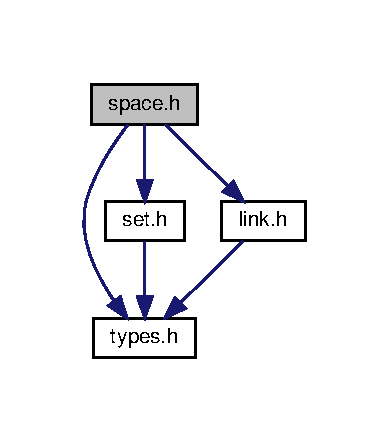
\includegraphics[width=187pt]{space_8h__incl}
\end{center}
\end{figure}
This graph shows which files directly or indirectly include this file\+:
\nopagebreak
\begin{figure}[H]
\begin{center}
\leavevmode
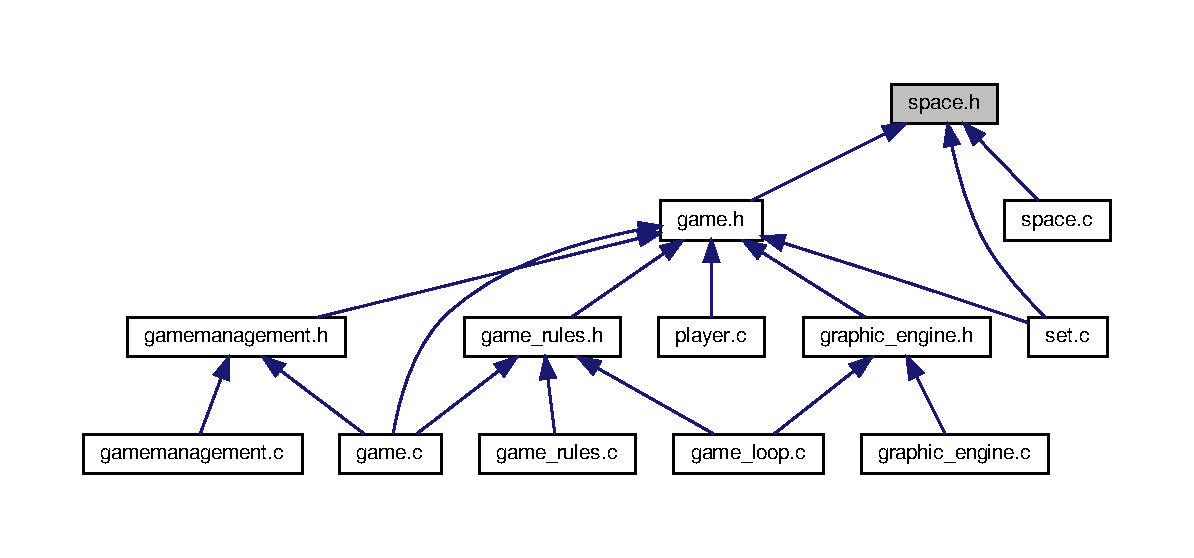
\includegraphics[width=350pt]{space_8h__dep__incl}
\end{center}
\end{figure}
\subsection*{Macros}
\begin{DoxyCompactItemize}
\item 
\mbox{\Hypertarget{space_8h_a5f54fd55f983a2e33ce076cd9f587e82}\label{space_8h_a5f54fd55f983a2e33ce076cd9f587e82}} 
\#define \hyperlink{space_8h_a5f54fd55f983a2e33ce076cd9f587e82}{M\+A\+X\+\_\+\+S\+P\+A\+C\+ES}~100
\begin{DoxyCompactList}\small\item\em defines the max of spaces \end{DoxyCompactList}\item 
\mbox{\Hypertarget{space_8h_a088cbe7c6f78264d46c2624194c5c680}\label{space_8h_a088cbe7c6f78264d46c2624194c5c680}} 
\#define \hyperlink{space_8h_a088cbe7c6f78264d46c2624194c5c680}{F\+I\+R\+S\+T\+\_\+\+S\+P\+A\+CE}~1
\begin{DoxyCompactList}\small\item\em defines fisrt space \end{DoxyCompactList}\end{DoxyCompactItemize}
\subsection*{Typedefs}
\begin{DoxyCompactItemize}
\item 
\mbox{\Hypertarget{space_8h_a67533ffc2b70463baecc38fb0629bbfc}\label{space_8h_a67533ffc2b70463baecc38fb0629bbfc}} 
typedef struct \hyperlink{struct__Space}{\+\_\+\+Space} \hyperlink{space_8h_a67533ffc2b70463baecc38fb0629bbfc}{Space}
\begin{DoxyCompactList}\small\item\em defines the space structure \end{DoxyCompactList}\end{DoxyCompactItemize}
\subsection*{Functions}
\begin{DoxyCompactItemize}
\item 
\hyperlink{space_8h_a67533ffc2b70463baecc38fb0629bbfc}{Space} $\ast$ \hyperlink{space_8h_a162866fcea156b800fd546d0ffd271c9}{space\+\_\+create} (\hyperlink{types_8h_a845e604fb28f7e3d97549da3448149d3}{Id} id)
\begin{DoxyCompactList}\small\item\em create the space in the game \end{DoxyCompactList}\item 
\hyperlink{types_8h_a32c27cc471df37f4fc818d65de0a56c4}{S\+T\+A\+T\+US} \hyperlink{space_8h_a5c70c70398923693ddbe4dfac8d72a0d}{space\+\_\+destroy} (\hyperlink{space_8h_a67533ffc2b70463baecc38fb0629bbfc}{Space} $\ast$space)
\begin{DoxyCompactList}\small\item\em destroy the space in the game \end{DoxyCompactList}\item 
\hyperlink{types_8h_a845e604fb28f7e3d97549da3448149d3}{Id} \hyperlink{space_8h_ac8ddfd0d8692fd852ee49698c446cb50}{space\+\_\+get\+\_\+id} (\hyperlink{space_8h_a67533ffc2b70463baecc38fb0629bbfc}{Space} $\ast$space)
\begin{DoxyCompactList}\small\item\em get the id of space \end{DoxyCompactList}\item 
\hyperlink{types_8h_a32c27cc471df37f4fc818d65de0a56c4}{S\+T\+A\+T\+US} \hyperlink{space_8h_aab5b468f9822ab78dbe16d1321870d93}{space\+\_\+set\+\_\+name} (\hyperlink{space_8h_a67533ffc2b70463baecc38fb0629bbfc}{Space} $\ast$space, char $\ast$name)
\begin{DoxyCompactList}\small\item\em set the id of space \end{DoxyCompactList}\item 
const char $\ast$ \hyperlink{space_8h_a310c540cd6e11073f7328add1f927001}{space\+\_\+get\+\_\+name} (\hyperlink{space_8h_a67533ffc2b70463baecc38fb0629bbfc}{Space} $\ast$space)
\begin{DoxyCompactList}\small\item\em get the name of space \end{DoxyCompactList}\item 
\hyperlink{types_8h_a32c27cc471df37f4fc818d65de0a56c4}{S\+T\+A\+T\+US} \hyperlink{space_8h_a9e6e3e3bac4996ac6b8bd555e52bfb26}{space\+\_\+set\+\_\+north} (\hyperlink{space_8h_a67533ffc2b70463baecc38fb0629bbfc}{Space} $\ast$space, \hyperlink{types_8h_a845e604fb28f7e3d97549da3448149d3}{Id} id)
\begin{DoxyCompactList}\small\item\em set the north id of space \end{DoxyCompactList}\item 
\hyperlink{types_8h_a845e604fb28f7e3d97549da3448149d3}{Id} \hyperlink{space_8h_ad331fba774897900f615d9d2e8d81a90}{space\+\_\+get\+\_\+north} (\hyperlink{space_8h_a67533ffc2b70463baecc38fb0629bbfc}{Space} $\ast$space)
\begin{DoxyCompactList}\small\item\em get the north id of space \end{DoxyCompactList}\item 
\hyperlink{types_8h_a32c27cc471df37f4fc818d65de0a56c4}{S\+T\+A\+T\+US} \hyperlink{space_8h_a422ab9f220b4c471c44256a27377de1a}{space\+\_\+set\+\_\+south} (\hyperlink{space_8h_a67533ffc2b70463baecc38fb0629bbfc}{Space} $\ast$space, \hyperlink{types_8h_a845e604fb28f7e3d97549da3448149d3}{Id} id)
\begin{DoxyCompactList}\small\item\em set the south id of space \end{DoxyCompactList}\item 
\hyperlink{types_8h_a845e604fb28f7e3d97549da3448149d3}{Id} \hyperlink{space_8h_a9b86e1335c423eaad832e50d4c12cf1f}{space\+\_\+get\+\_\+south} (\hyperlink{space_8h_a67533ffc2b70463baecc38fb0629bbfc}{Space} $\ast$space)
\begin{DoxyCompactList}\small\item\em get the south id of space \end{DoxyCompactList}\item 
\hyperlink{types_8h_a32c27cc471df37f4fc818d65de0a56c4}{S\+T\+A\+T\+US} \hyperlink{space_8h_a860a8f3e0227955ad56d1a12f0bdc44a}{space\+\_\+set\+\_\+east} (\hyperlink{space_8h_a67533ffc2b70463baecc38fb0629bbfc}{Space} $\ast$space, \hyperlink{types_8h_a845e604fb28f7e3d97549da3448149d3}{Id} id)
\begin{DoxyCompactList}\small\item\em set the east id of space \end{DoxyCompactList}\item 
\hyperlink{types_8h_a845e604fb28f7e3d97549da3448149d3}{Id} \hyperlink{space_8h_a978a22b77f74bb2dab68a00571abbe0b}{space\+\_\+get\+\_\+east} (\hyperlink{space_8h_a67533ffc2b70463baecc38fb0629bbfc}{Space} $\ast$space)
\begin{DoxyCompactList}\small\item\em get the east id of space \end{DoxyCompactList}\item 
\hyperlink{types_8h_a32c27cc471df37f4fc818d65de0a56c4}{S\+T\+A\+T\+US} \hyperlink{space_8h_ad44b14cb38902cf31fa1f341beaab0db}{space\+\_\+set\+\_\+west} (\hyperlink{space_8h_a67533ffc2b70463baecc38fb0629bbfc}{Space} $\ast$space, \hyperlink{types_8h_a845e604fb28f7e3d97549da3448149d3}{Id} id)
\begin{DoxyCompactList}\small\item\em set the west id of space \end{DoxyCompactList}\item 
\hyperlink{types_8h_a845e604fb28f7e3d97549da3448149d3}{Id} \hyperlink{space_8h_af495ebfd5d13eba1a48cebd10992a17f}{space\+\_\+get\+\_\+west} (\hyperlink{space_8h_a67533ffc2b70463baecc38fb0629bbfc}{Space} $\ast$space)
\begin{DoxyCompactList}\small\item\em get the west id of space \end{DoxyCompactList}\item 
\hyperlink{types_8h_a32c27cc471df37f4fc818d65de0a56c4}{S\+T\+A\+T\+US} \hyperlink{space_8h_a510c703a1eeac8965932394a900a43cc}{space\+\_\+set\+\_\+object} (\hyperlink{space_8h_a67533ffc2b70463baecc38fb0629bbfc}{Space} $\ast$space, \hyperlink{types_8h_a845e604fb28f7e3d97549da3448149d3}{Id} value)
\begin{DoxyCompactList}\small\item\em set the object to the space \end{DoxyCompactList}\item 
\hyperlink{set_8h_a6d3b7f7c92cbb4577ef3ef7ddbf93161}{Set} $\ast$ \hyperlink{space_8h_ab24abae4e127bf0bca596cd71ba3aad6}{space\+\_\+get\+\_\+object} (\hyperlink{space_8h_a67533ffc2b70463baecc38fb0629bbfc}{Space} $\ast$space)
\begin{DoxyCompactList}\small\item\em get the object to the space \end{DoxyCompactList}\item 
\hyperlink{types_8h_a32c27cc471df37f4fc818d65de0a56c4}{S\+T\+A\+T\+US} \hyperlink{space_8h_a18eca058da6cdf20ae5eda9d122d992e}{space\+\_\+print} (\hyperlink{space_8h_a67533ffc2b70463baecc38fb0629bbfc}{Space} $\ast$space)
\begin{DoxyCompactList}\small\item\em print the object of the space \end{DoxyCompactList}\item 
char $\ast$ \hyperlink{space_8h_abc33179385bc05971038bf0eb68b2d3a}{space\+\_\+get\+\_\+gdesc} (\hyperlink{space_8h_a67533ffc2b70463baecc38fb0629bbfc}{Space} $\ast$space, int i)
\begin{DoxyCompactList}\small\item\em get the objec gdesc \end{DoxyCompactList}\item 
char $\ast$ \hyperlink{space_8h_ae8a9b9294e8b285d680d3ce2c470f4b9}{space\+\_\+create\+\_\+gdesc} ()
\begin{DoxyCompactList}\small\item\em set the objec gdesc \end{DoxyCompactList}\item 
\hyperlink{types_8h_a32c27cc471df37f4fc818d65de0a56c4}{S\+T\+A\+T\+US} \hyperlink{space_8h_a3723b291fc3cbbd723622ee0f9b52a62}{space\+\_\+set\+\_\+gdesc} (\hyperlink{space_8h_a67533ffc2b70463baecc38fb0629bbfc}{Space} $\ast$space, char $\ast$str, int i)
\begin{DoxyCompactList}\small\item\em set the objec gdesc to space \end{DoxyCompactList}\item 
\hyperlink{types_8h_a32c27cc471df37f4fc818d65de0a56c4}{S\+T\+A\+T\+US} \hyperlink{space_8h_ac69528ddf930a534d57c5d1d74691f1d}{space\+\_\+set\+\_\+description} (\hyperlink{space_8h_a67533ffc2b70463baecc38fb0629bbfc}{Space} $\ast$space, char $\ast$desc)
\begin{DoxyCompactList}\small\item\em set the descripcion of objects \end{DoxyCompactList}\item 
const char $\ast$ \hyperlink{space_8h_a51e854a2f9b35bd39e60c04ec5f03abd}{space\+\_\+get\+\_\+description} (\hyperlink{space_8h_a67533ffc2b70463baecc38fb0629bbfc}{Space} $\ast$space)
\begin{DoxyCompactList}\small\item\em get the descripcion of objects \end{DoxyCompactList}\end{DoxyCompactItemize}


\subsection{Detailed Description}
It defines a space. 

\begin{DoxyAuthor}{Author}
\end{DoxyAuthor}
\begin{DoxyVersion}{Version}
1.\+0 
\end{DoxyVersion}
\begin{DoxyDate}{Date}
04-\/02-\/2019 
\end{DoxyDate}
\begin{DoxyCopyright}{Copyright}
G\+NU Public License 
\end{DoxyCopyright}


\subsection{Function Documentation}
\mbox{\Hypertarget{space_8h_a162866fcea156b800fd546d0ffd271c9}\label{space_8h_a162866fcea156b800fd546d0ffd271c9}} 
\index{space.\+h@{space.\+h}!space\+\_\+create@{space\+\_\+create}}
\index{space\+\_\+create@{space\+\_\+create}!space.\+h@{space.\+h}}
\subsubsection{\texorpdfstring{space\+\_\+create()}{space\_create()}}
{\footnotesize\ttfamily \hyperlink{space_8h_a67533ffc2b70463baecc38fb0629bbfc}{Space}$\ast$ space\+\_\+create (\begin{DoxyParamCaption}\item[{\hyperlink{types_8h_a845e604fb28f7e3d97549da3448149d3}{Id}}]{id }\end{DoxyParamCaption})}



create the space in the game 


\begin{DoxyParams}{Parameters}
{\em id} & \\
\hline
\end{DoxyParams}
\begin{DoxyReturn}{Returns}
space or in case of error N\+U\+LL 
\end{DoxyReturn}
\mbox{\Hypertarget{space_8h_ae8a9b9294e8b285d680d3ce2c470f4b9}\label{space_8h_ae8a9b9294e8b285d680d3ce2c470f4b9}} 
\index{space.\+h@{space.\+h}!space\+\_\+create\+\_\+gdesc@{space\+\_\+create\+\_\+gdesc}}
\index{space\+\_\+create\+\_\+gdesc@{space\+\_\+create\+\_\+gdesc}!space.\+h@{space.\+h}}
\subsubsection{\texorpdfstring{space\+\_\+create\+\_\+gdesc()}{space\_create\_gdesc()}}
{\footnotesize\ttfamily char$\ast$ space\+\_\+create\+\_\+gdesc (\begin{DoxyParamCaption}{ }\end{DoxyParamCaption})}



set the objec gdesc 

\begin{DoxyReturn}{Returns}
char or in case of error N\+U\+LL 
\end{DoxyReturn}
\mbox{\Hypertarget{space_8h_a5c70c70398923693ddbe4dfac8d72a0d}\label{space_8h_a5c70c70398923693ddbe4dfac8d72a0d}} 
\index{space.\+h@{space.\+h}!space\+\_\+destroy@{space\+\_\+destroy}}
\index{space\+\_\+destroy@{space\+\_\+destroy}!space.\+h@{space.\+h}}
\subsubsection{\texorpdfstring{space\+\_\+destroy()}{space\_destroy()}}
{\footnotesize\ttfamily \hyperlink{types_8h_a32c27cc471df37f4fc818d65de0a56c4}{S\+T\+A\+T\+US} space\+\_\+destroy (\begin{DoxyParamCaption}\item[{\hyperlink{space_8h_a67533ffc2b70463baecc38fb0629bbfc}{Space} $\ast$}]{space }\end{DoxyParamCaption})}



destroy the space in the game 


\begin{DoxyParams}{Parameters}
{\em space} & \\
\hline
\end{DoxyParams}
\begin{DoxyReturn}{Returns}
OK, or E\+R\+R\+OR 
\end{DoxyReturn}
\mbox{\Hypertarget{space_8h_a51e854a2f9b35bd39e60c04ec5f03abd}\label{space_8h_a51e854a2f9b35bd39e60c04ec5f03abd}} 
\index{space.\+h@{space.\+h}!space\+\_\+get\+\_\+description@{space\+\_\+get\+\_\+description}}
\index{space\+\_\+get\+\_\+description@{space\+\_\+get\+\_\+description}!space.\+h@{space.\+h}}
\subsubsection{\texorpdfstring{space\+\_\+get\+\_\+description()}{space\_get\_description()}}
{\footnotesize\ttfamily const char$\ast$ space\+\_\+get\+\_\+description (\begin{DoxyParamCaption}\item[{\hyperlink{space_8h_a67533ffc2b70463baecc38fb0629bbfc}{Space} $\ast$}]{space }\end{DoxyParamCaption})}



get the descripcion of objects 


\begin{DoxyParams}{Parameters}
{\em space} & \\
\hline
\end{DoxyParams}
\begin{DoxyReturn}{Returns}
char or in case of error N\+U\+LL 
\end{DoxyReturn}
\mbox{\Hypertarget{space_8h_a978a22b77f74bb2dab68a00571abbe0b}\label{space_8h_a978a22b77f74bb2dab68a00571abbe0b}} 
\index{space.\+h@{space.\+h}!space\+\_\+get\+\_\+east@{space\+\_\+get\+\_\+east}}
\index{space\+\_\+get\+\_\+east@{space\+\_\+get\+\_\+east}!space.\+h@{space.\+h}}
\subsubsection{\texorpdfstring{space\+\_\+get\+\_\+east()}{space\_get\_east()}}
{\footnotesize\ttfamily \hyperlink{types_8h_a845e604fb28f7e3d97549da3448149d3}{Id} space\+\_\+get\+\_\+east (\begin{DoxyParamCaption}\item[{\hyperlink{space_8h_a67533ffc2b70463baecc38fb0629bbfc}{Space} $\ast$}]{space }\end{DoxyParamCaption})}



get the east id of space 


\begin{DoxyParams}{Parameters}
{\em space} & \\
\hline
\end{DoxyParams}
\begin{DoxyReturn}{Returns}
id or in case of error N\+U\+LL 
\end{DoxyReturn}
\mbox{\Hypertarget{space_8h_abc33179385bc05971038bf0eb68b2d3a}\label{space_8h_abc33179385bc05971038bf0eb68b2d3a}} 
\index{space.\+h@{space.\+h}!space\+\_\+get\+\_\+gdesc@{space\+\_\+get\+\_\+gdesc}}
\index{space\+\_\+get\+\_\+gdesc@{space\+\_\+get\+\_\+gdesc}!space.\+h@{space.\+h}}
\subsubsection{\texorpdfstring{space\+\_\+get\+\_\+gdesc()}{space\_get\_gdesc()}}
{\footnotesize\ttfamily char$\ast$ space\+\_\+get\+\_\+gdesc (\begin{DoxyParamCaption}\item[{\hyperlink{space_8h_a67533ffc2b70463baecc38fb0629bbfc}{Space} $\ast$}]{space,  }\item[{int}]{i }\end{DoxyParamCaption})}



get the objec gdesc 


\begin{DoxyParams}{Parameters}
{\em space} & \\
\hline
{\em i} & \\
\hline
\end{DoxyParams}
\begin{DoxyReturn}{Returns}
char or in case of error N\+U\+LL 
\end{DoxyReturn}
\mbox{\Hypertarget{space_8h_ac8ddfd0d8692fd852ee49698c446cb50}\label{space_8h_ac8ddfd0d8692fd852ee49698c446cb50}} 
\index{space.\+h@{space.\+h}!space\+\_\+get\+\_\+id@{space\+\_\+get\+\_\+id}}
\index{space\+\_\+get\+\_\+id@{space\+\_\+get\+\_\+id}!space.\+h@{space.\+h}}
\subsubsection{\texorpdfstring{space\+\_\+get\+\_\+id()}{space\_get\_id()}}
{\footnotesize\ttfamily \hyperlink{types_8h_a845e604fb28f7e3d97549da3448149d3}{Id} space\+\_\+get\+\_\+id (\begin{DoxyParamCaption}\item[{\hyperlink{space_8h_a67533ffc2b70463baecc38fb0629bbfc}{Space} $\ast$}]{space }\end{DoxyParamCaption})}



get the id of space 


\begin{DoxyParams}{Parameters}
{\em space} & \\
\hline
\end{DoxyParams}
\begin{DoxyReturn}{Returns}
id or in case of error N\+U\+LL 
\end{DoxyReturn}
\mbox{\Hypertarget{space_8h_a310c540cd6e11073f7328add1f927001}\label{space_8h_a310c540cd6e11073f7328add1f927001}} 
\index{space.\+h@{space.\+h}!space\+\_\+get\+\_\+name@{space\+\_\+get\+\_\+name}}
\index{space\+\_\+get\+\_\+name@{space\+\_\+get\+\_\+name}!space.\+h@{space.\+h}}
\subsubsection{\texorpdfstring{space\+\_\+get\+\_\+name()}{space\_get\_name()}}
{\footnotesize\ttfamily const char$\ast$ space\+\_\+get\+\_\+name (\begin{DoxyParamCaption}\item[{\hyperlink{space_8h_a67533ffc2b70463baecc38fb0629bbfc}{Space} $\ast$}]{space }\end{DoxyParamCaption})}



get the name of space 


\begin{DoxyParams}{Parameters}
{\em space} & \\
\hline
\end{DoxyParams}
\begin{DoxyReturn}{Returns}
name of space or in case of error N\+U\+LL 
\end{DoxyReturn}
\mbox{\Hypertarget{space_8h_ad331fba774897900f615d9d2e8d81a90}\label{space_8h_ad331fba774897900f615d9d2e8d81a90}} 
\index{space.\+h@{space.\+h}!space\+\_\+get\+\_\+north@{space\+\_\+get\+\_\+north}}
\index{space\+\_\+get\+\_\+north@{space\+\_\+get\+\_\+north}!space.\+h@{space.\+h}}
\subsubsection{\texorpdfstring{space\+\_\+get\+\_\+north()}{space\_get\_north()}}
{\footnotesize\ttfamily \hyperlink{types_8h_a845e604fb28f7e3d97549da3448149d3}{Id} space\+\_\+get\+\_\+north (\begin{DoxyParamCaption}\item[{\hyperlink{space_8h_a67533ffc2b70463baecc38fb0629bbfc}{Space} $\ast$}]{space }\end{DoxyParamCaption})}



get the north id of space 


\begin{DoxyParams}{Parameters}
{\em space} & \\
\hline
\end{DoxyParams}
\begin{DoxyReturn}{Returns}
id or in case of error N\+U\+LL 
\end{DoxyReturn}
\mbox{\Hypertarget{space_8h_ab24abae4e127bf0bca596cd71ba3aad6}\label{space_8h_ab24abae4e127bf0bca596cd71ba3aad6}} 
\index{space.\+h@{space.\+h}!space\+\_\+get\+\_\+object@{space\+\_\+get\+\_\+object}}
\index{space\+\_\+get\+\_\+object@{space\+\_\+get\+\_\+object}!space.\+h@{space.\+h}}
\subsubsection{\texorpdfstring{space\+\_\+get\+\_\+object()}{space\_get\_object()}}
{\footnotesize\ttfamily \hyperlink{set_8h_a6d3b7f7c92cbb4577ef3ef7ddbf93161}{Set}$\ast$ space\+\_\+get\+\_\+object (\begin{DoxyParamCaption}\item[{\hyperlink{space_8h_a67533ffc2b70463baecc38fb0629bbfc}{Space} $\ast$}]{space }\end{DoxyParamCaption})}



get the object to the space 


\begin{DoxyParams}{Parameters}
{\em space} & \\
\hline
\end{DoxyParams}
\begin{DoxyReturn}{Returns}
set or in case of error N\+U\+LL 
\end{DoxyReturn}
\mbox{\Hypertarget{space_8h_a9b86e1335c423eaad832e50d4c12cf1f}\label{space_8h_a9b86e1335c423eaad832e50d4c12cf1f}} 
\index{space.\+h@{space.\+h}!space\+\_\+get\+\_\+south@{space\+\_\+get\+\_\+south}}
\index{space\+\_\+get\+\_\+south@{space\+\_\+get\+\_\+south}!space.\+h@{space.\+h}}
\subsubsection{\texorpdfstring{space\+\_\+get\+\_\+south()}{space\_get\_south()}}
{\footnotesize\ttfamily \hyperlink{types_8h_a845e604fb28f7e3d97549da3448149d3}{Id} space\+\_\+get\+\_\+south (\begin{DoxyParamCaption}\item[{\hyperlink{space_8h_a67533ffc2b70463baecc38fb0629bbfc}{Space} $\ast$}]{space }\end{DoxyParamCaption})}



get the south id of space 


\begin{DoxyParams}{Parameters}
{\em space} & \\
\hline
\end{DoxyParams}
\begin{DoxyReturn}{Returns}
id or in case of error N\+U\+LL 
\end{DoxyReturn}
\mbox{\Hypertarget{space_8h_af495ebfd5d13eba1a48cebd10992a17f}\label{space_8h_af495ebfd5d13eba1a48cebd10992a17f}} 
\index{space.\+h@{space.\+h}!space\+\_\+get\+\_\+west@{space\+\_\+get\+\_\+west}}
\index{space\+\_\+get\+\_\+west@{space\+\_\+get\+\_\+west}!space.\+h@{space.\+h}}
\subsubsection{\texorpdfstring{space\+\_\+get\+\_\+west()}{space\_get\_west()}}
{\footnotesize\ttfamily \hyperlink{types_8h_a845e604fb28f7e3d97549da3448149d3}{Id} space\+\_\+get\+\_\+west (\begin{DoxyParamCaption}\item[{\hyperlink{space_8h_a67533ffc2b70463baecc38fb0629bbfc}{Space} $\ast$}]{space }\end{DoxyParamCaption})}



get the west id of space 


\begin{DoxyParams}{Parameters}
{\em space} & \\
\hline
\end{DoxyParams}
\begin{DoxyReturn}{Returns}
id or in case of error N\+U\+LL 
\end{DoxyReturn}
\mbox{\Hypertarget{space_8h_a18eca058da6cdf20ae5eda9d122d992e}\label{space_8h_a18eca058da6cdf20ae5eda9d122d992e}} 
\index{space.\+h@{space.\+h}!space\+\_\+print@{space\+\_\+print}}
\index{space\+\_\+print@{space\+\_\+print}!space.\+h@{space.\+h}}
\subsubsection{\texorpdfstring{space\+\_\+print()}{space\_print()}}
{\footnotesize\ttfamily \hyperlink{types_8h_a32c27cc471df37f4fc818d65de0a56c4}{S\+T\+A\+T\+US} space\+\_\+print (\begin{DoxyParamCaption}\item[{\hyperlink{space_8h_a67533ffc2b70463baecc38fb0629bbfc}{Space} $\ast$}]{space }\end{DoxyParamCaption})}



print the object of the space 


\begin{DoxyParams}{Parameters}
{\em space} & \\
\hline
\end{DoxyParams}
\begin{DoxyReturn}{Returns}
OK, or E\+R\+R\+OR 
\end{DoxyReturn}
\mbox{\Hypertarget{space_8h_ac69528ddf930a534d57c5d1d74691f1d}\label{space_8h_ac69528ddf930a534d57c5d1d74691f1d}} 
\index{space.\+h@{space.\+h}!space\+\_\+set\+\_\+description@{space\+\_\+set\+\_\+description}}
\index{space\+\_\+set\+\_\+description@{space\+\_\+set\+\_\+description}!space.\+h@{space.\+h}}
\subsubsection{\texorpdfstring{space\+\_\+set\+\_\+description()}{space\_set\_description()}}
{\footnotesize\ttfamily \hyperlink{types_8h_a32c27cc471df37f4fc818d65de0a56c4}{S\+T\+A\+T\+US} space\+\_\+set\+\_\+description (\begin{DoxyParamCaption}\item[{\hyperlink{space_8h_a67533ffc2b70463baecc38fb0629bbfc}{Space} $\ast$}]{space,  }\item[{char $\ast$}]{desc }\end{DoxyParamCaption})}



set the descripcion of objects 


\begin{DoxyParams}{Parameters}
{\em space} & \\
\hline
{\em desc} & \\
\hline
\end{DoxyParams}
\begin{DoxyReturn}{Returns}
OK, or E\+R\+R\+OR 
\end{DoxyReturn}
\mbox{\Hypertarget{space_8h_a860a8f3e0227955ad56d1a12f0bdc44a}\label{space_8h_a860a8f3e0227955ad56d1a12f0bdc44a}} 
\index{space.\+h@{space.\+h}!space\+\_\+set\+\_\+east@{space\+\_\+set\+\_\+east}}
\index{space\+\_\+set\+\_\+east@{space\+\_\+set\+\_\+east}!space.\+h@{space.\+h}}
\subsubsection{\texorpdfstring{space\+\_\+set\+\_\+east()}{space\_set\_east()}}
{\footnotesize\ttfamily \hyperlink{types_8h_a32c27cc471df37f4fc818d65de0a56c4}{S\+T\+A\+T\+US} space\+\_\+set\+\_\+east (\begin{DoxyParamCaption}\item[{\hyperlink{space_8h_a67533ffc2b70463baecc38fb0629bbfc}{Space} $\ast$}]{space,  }\item[{\hyperlink{types_8h_a845e604fb28f7e3d97549da3448149d3}{Id}}]{id }\end{DoxyParamCaption})}



set the east id of space 


\begin{DoxyParams}{Parameters}
{\em space} & \\
\hline
{\em id} & \\
\hline
\end{DoxyParams}
\begin{DoxyReturn}{Returns}
OK, or E\+R\+R\+OR 
\end{DoxyReturn}
\mbox{\Hypertarget{space_8h_a3723b291fc3cbbd723622ee0f9b52a62}\label{space_8h_a3723b291fc3cbbd723622ee0f9b52a62}} 
\index{space.\+h@{space.\+h}!space\+\_\+set\+\_\+gdesc@{space\+\_\+set\+\_\+gdesc}}
\index{space\+\_\+set\+\_\+gdesc@{space\+\_\+set\+\_\+gdesc}!space.\+h@{space.\+h}}
\subsubsection{\texorpdfstring{space\+\_\+set\+\_\+gdesc()}{space\_set\_gdesc()}}
{\footnotesize\ttfamily \hyperlink{types_8h_a32c27cc471df37f4fc818d65de0a56c4}{S\+T\+A\+T\+US} space\+\_\+set\+\_\+gdesc (\begin{DoxyParamCaption}\item[{\hyperlink{space_8h_a67533ffc2b70463baecc38fb0629bbfc}{Space} $\ast$}]{space,  }\item[{char $\ast$}]{str,  }\item[{int}]{i }\end{DoxyParamCaption})}



set the objec gdesc to space 


\begin{DoxyParams}{Parameters}
{\em space} & \\
\hline
{\em i} & \\
\hline
{\em str} & \\
\hline
\end{DoxyParams}
\begin{DoxyReturn}{Returns}
OK, or E\+R\+R\+OR 
\end{DoxyReturn}
\mbox{\Hypertarget{space_8h_aab5b468f9822ab78dbe16d1321870d93}\label{space_8h_aab5b468f9822ab78dbe16d1321870d93}} 
\index{space.\+h@{space.\+h}!space\+\_\+set\+\_\+name@{space\+\_\+set\+\_\+name}}
\index{space\+\_\+set\+\_\+name@{space\+\_\+set\+\_\+name}!space.\+h@{space.\+h}}
\subsubsection{\texorpdfstring{space\+\_\+set\+\_\+name()}{space\_set\_name()}}
{\footnotesize\ttfamily \hyperlink{types_8h_a32c27cc471df37f4fc818d65de0a56c4}{S\+T\+A\+T\+US} space\+\_\+set\+\_\+name (\begin{DoxyParamCaption}\item[{\hyperlink{space_8h_a67533ffc2b70463baecc38fb0629bbfc}{Space} $\ast$}]{space,  }\item[{char $\ast$}]{name }\end{DoxyParamCaption})}



set the id of space 


\begin{DoxyParams}{Parameters}
{\em space} & \\
\hline
{\em name} & \\
\hline
\end{DoxyParams}
\begin{DoxyReturn}{Returns}
OK, or E\+R\+R\+OR 
\end{DoxyReturn}
\mbox{\Hypertarget{space_8h_a9e6e3e3bac4996ac6b8bd555e52bfb26}\label{space_8h_a9e6e3e3bac4996ac6b8bd555e52bfb26}} 
\index{space.\+h@{space.\+h}!space\+\_\+set\+\_\+north@{space\+\_\+set\+\_\+north}}
\index{space\+\_\+set\+\_\+north@{space\+\_\+set\+\_\+north}!space.\+h@{space.\+h}}
\subsubsection{\texorpdfstring{space\+\_\+set\+\_\+north()}{space\_set\_north()}}
{\footnotesize\ttfamily \hyperlink{types_8h_a32c27cc471df37f4fc818d65de0a56c4}{S\+T\+A\+T\+US} space\+\_\+set\+\_\+north (\begin{DoxyParamCaption}\item[{\hyperlink{space_8h_a67533ffc2b70463baecc38fb0629bbfc}{Space} $\ast$}]{space,  }\item[{\hyperlink{types_8h_a845e604fb28f7e3d97549da3448149d3}{Id}}]{id }\end{DoxyParamCaption})}



set the north id of space 


\begin{DoxyParams}{Parameters}
{\em space} & \\
\hline
{\em id} & \\
\hline
\end{DoxyParams}
\begin{DoxyReturn}{Returns}
OK, or E\+R\+R\+OR 
\end{DoxyReturn}
\mbox{\Hypertarget{space_8h_a510c703a1eeac8965932394a900a43cc}\label{space_8h_a510c703a1eeac8965932394a900a43cc}} 
\index{space.\+h@{space.\+h}!space\+\_\+set\+\_\+object@{space\+\_\+set\+\_\+object}}
\index{space\+\_\+set\+\_\+object@{space\+\_\+set\+\_\+object}!space.\+h@{space.\+h}}
\subsubsection{\texorpdfstring{space\+\_\+set\+\_\+object()}{space\_set\_object()}}
{\footnotesize\ttfamily \hyperlink{types_8h_a32c27cc471df37f4fc818d65de0a56c4}{S\+T\+A\+T\+US} space\+\_\+set\+\_\+object (\begin{DoxyParamCaption}\item[{\hyperlink{space_8h_a67533ffc2b70463baecc38fb0629bbfc}{Space} $\ast$}]{space,  }\item[{\hyperlink{types_8h_a845e604fb28f7e3d97549da3448149d3}{Id}}]{value }\end{DoxyParamCaption})}



set the object to the space 


\begin{DoxyParams}{Parameters}
{\em space} & \\
\hline
{\em value} & \\
\hline
\end{DoxyParams}
\begin{DoxyReturn}{Returns}
OK, or E\+R\+R\+OR 
\end{DoxyReturn}
\mbox{\Hypertarget{space_8h_a422ab9f220b4c471c44256a27377de1a}\label{space_8h_a422ab9f220b4c471c44256a27377de1a}} 
\index{space.\+h@{space.\+h}!space\+\_\+set\+\_\+south@{space\+\_\+set\+\_\+south}}
\index{space\+\_\+set\+\_\+south@{space\+\_\+set\+\_\+south}!space.\+h@{space.\+h}}
\subsubsection{\texorpdfstring{space\+\_\+set\+\_\+south()}{space\_set\_south()}}
{\footnotesize\ttfamily \hyperlink{types_8h_a32c27cc471df37f4fc818d65de0a56c4}{S\+T\+A\+T\+US} space\+\_\+set\+\_\+south (\begin{DoxyParamCaption}\item[{\hyperlink{space_8h_a67533ffc2b70463baecc38fb0629bbfc}{Space} $\ast$}]{space,  }\item[{\hyperlink{types_8h_a845e604fb28f7e3d97549da3448149d3}{Id}}]{id }\end{DoxyParamCaption})}



set the south id of space 


\begin{DoxyParams}{Parameters}
{\em space} & \\
\hline
{\em id} & \\
\hline
\end{DoxyParams}
\begin{DoxyReturn}{Returns}
OK, or E\+R\+R\+OR 
\end{DoxyReturn}
\mbox{\Hypertarget{space_8h_ad44b14cb38902cf31fa1f341beaab0db}\label{space_8h_ad44b14cb38902cf31fa1f341beaab0db}} 
\index{space.\+h@{space.\+h}!space\+\_\+set\+\_\+west@{space\+\_\+set\+\_\+west}}
\index{space\+\_\+set\+\_\+west@{space\+\_\+set\+\_\+west}!space.\+h@{space.\+h}}
\subsubsection{\texorpdfstring{space\+\_\+set\+\_\+west()}{space\_set\_west()}}
{\footnotesize\ttfamily \hyperlink{types_8h_a32c27cc471df37f4fc818d65de0a56c4}{S\+T\+A\+T\+US} space\+\_\+set\+\_\+west (\begin{DoxyParamCaption}\item[{\hyperlink{space_8h_a67533ffc2b70463baecc38fb0629bbfc}{Space} $\ast$}]{space,  }\item[{\hyperlink{types_8h_a845e604fb28f7e3d97549da3448149d3}{Id}}]{id }\end{DoxyParamCaption})}



set the west id of space 


\begin{DoxyParams}{Parameters}
{\em space} & \\
\hline
{\em id} & \\
\hline
\end{DoxyParams}
\begin{DoxyReturn}{Returns}
OK, or E\+R\+R\+OR 
\end{DoxyReturn}


\hypertarget{types_8h}{\section{include/types.h File Reference}
\label{types_8h}\index{include/types.\+h@{include/types.\+h}}
}


It defines common types.  


This graph shows which files directly or indirectly include this file\+:
\nopagebreak
\begin{figure}[H]
\begin{center}
\leavevmode
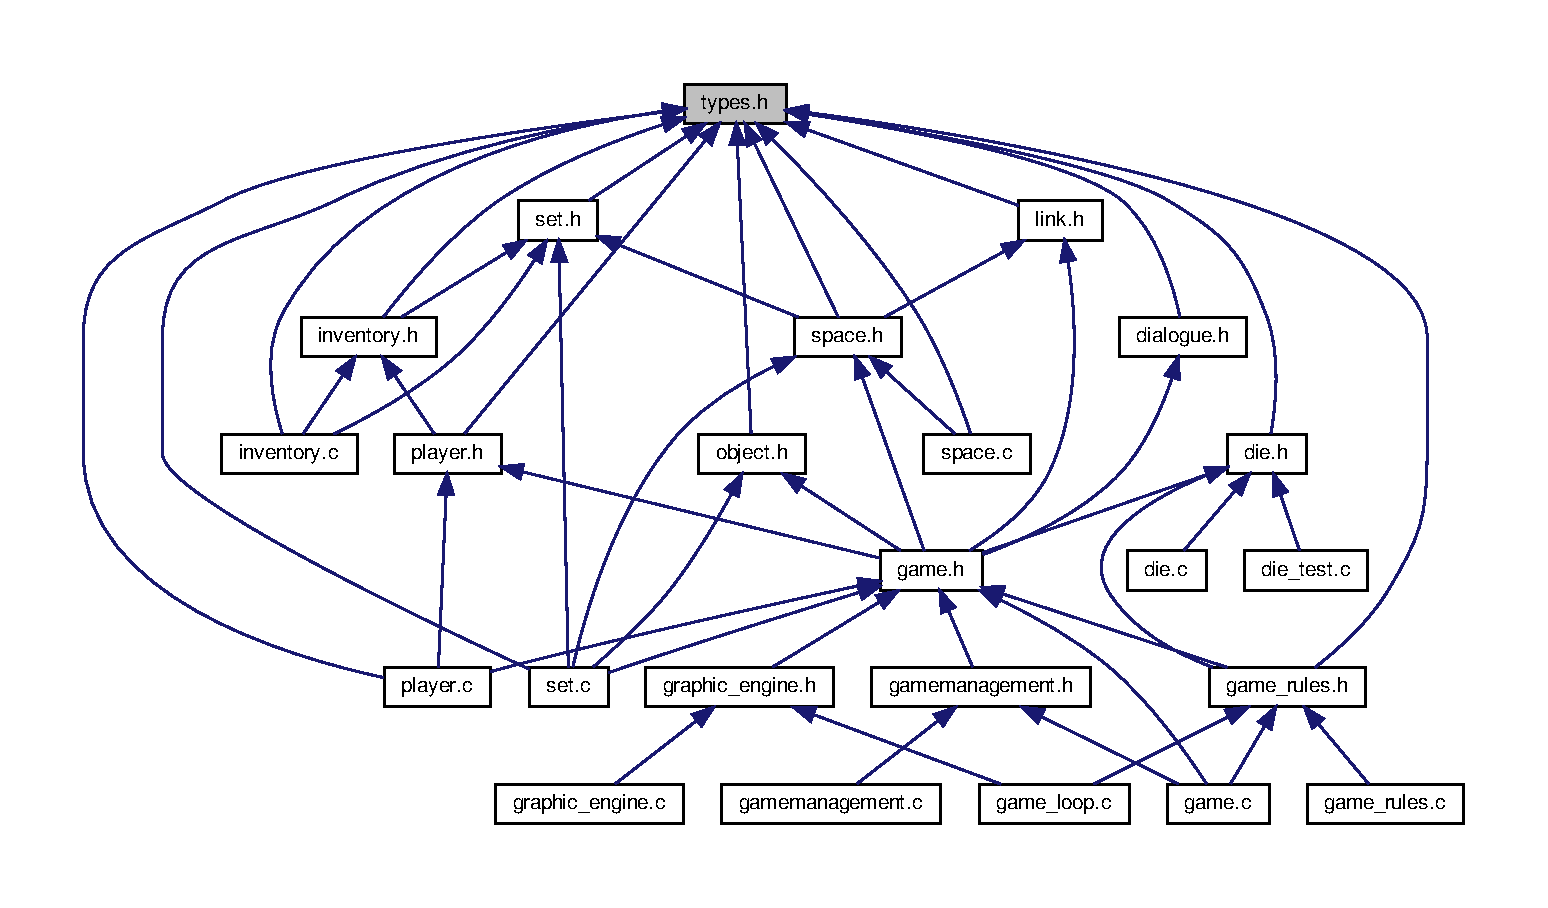
\includegraphics[width=350pt]{types_8h__dep__incl}
\end{center}
\end{figure}
\subsection*{Macros}
\begin{DoxyCompactItemize}
\item 
\#define \hyperlink{types_8h_a92ed8507d1cd2331ad09275c5c4c1c89}{W\+O\+R\+D\+\_\+\+S\+I\+Z\+E}~1000
\item 
\#define \hyperlink{types_8h_a642e16f35aa1e585c25e405ede76e115}{N\+O\+\_\+\+I\+D}~-\/1
\end{DoxyCompactItemize}
\subsection*{Typedefs}
\begin{DoxyCompactItemize}
\item 
\hypertarget{types_8h_a845e604fb28f7e3d97549da3448149d3}{typedef long \hyperlink{types_8h_a845e604fb28f7e3d97549da3448149d3}{Id}}\label{types_8h_a845e604fb28f7e3d97549da3448149d3}

\begin{DoxyCompactList}\small\item\em deifinicion del tipo de id \end{DoxyCompactList}\end{DoxyCompactItemize}
\subsection*{Enumerations}
\begin{DoxyCompactItemize}
\item 
\hypertarget{types_8h_a3e5b8192e7d9ffaf3542f1210aec18dd}{enum \hyperlink{types_8h_a3e5b8192e7d9ffaf3542f1210aec18dd}{B\+O\+O\+L} \{ {\bfseries F\+A\+L\+S\+E}, 
{\bfseries T\+R\+U\+E}
 \}}\label{types_8h_a3e5b8192e7d9ffaf3542f1210aec18dd}

\begin{DoxyCompactList}\small\item\em deifinicion del tipo de B\+O\+O\+L \end{DoxyCompactList}\item 
\hypertarget{types_8h_a32c27cc471df37f4fc818d65de0a56c4}{enum \hyperlink{types_8h_a32c27cc471df37f4fc818d65de0a56c4}{S\+T\+A\+T\+U\+S} \{ {\bfseries E\+R\+R\+O\+R}, 
{\bfseries O\+K}
 \}}\label{types_8h_a32c27cc471df37f4fc818d65de0a56c4}

\begin{DoxyCompactList}\small\item\em deifinicion del tipo status, O\+K o E\+R\+R\+O\+R \end{DoxyCompactList}\item 
\hypertarget{types_8h_aa268a41a13430b18e933ed40207178d0}{enum \hyperlink{types_8h_aa268a41a13430b18e933ed40207178d0}{D\+I\+R\+E\+C\+T\+I\+O\+N} \{ {\bfseries N}, 
{\bfseries S}, 
{\bfseries E}, 
{\bfseries W}
 \}}\label{types_8h_aa268a41a13430b18e933ed40207178d0}

\begin{DoxyCompactList}\small\item\em lista de direcciones de desplazamiento \end{DoxyCompactList}\item 
\hypertarget{types_8h_a4eb959f56c9de4fb79f4891902033093}{enum \hyperlink{types_8h_a4eb959f56c9de4fb79f4891902033093}{D\+O\+O\+R} \{ {\bfseries O\+P\+E\+N\+N\+E\+D}, 
{\bfseries C\+L\+O\+S\+E\+D}
 \}}\label{types_8h_a4eb959f56c9de4fb79f4891902033093}

\begin{DoxyCompactList}\small\item\em deifinicion del tipo de la puerta de los links \end{DoxyCompactList}\end{DoxyCompactItemize}


\subsection{Detailed Description}
It defines common types. 

\begin{DoxyAuthor}{Author}
Julia Simon 
\end{DoxyAuthor}
\begin{DoxyVersion}{Version}
1.\+0 
\end{DoxyVersion}
\begin{DoxyDate}{Date}
30-\/03-\/2018 
\end{DoxyDate}


\subsection{Macro Definition Documentation}
\hypertarget{types_8h_a642e16f35aa1e585c25e405ede76e115}{\index{types.\+h@{types.\+h}!N\+O\+\_\+\+I\+D@{N\+O\+\_\+\+I\+D}}
\index{N\+O\+\_\+\+I\+D@{N\+O\+\_\+\+I\+D}!types.\+h@{types.\+h}}
\subsubsection[{N\+O\+\_\+\+I\+D}]{\setlength{\rightskip}{0pt plus 5cm}\#define N\+O\+\_\+\+I\+D~-\/1}}\label{types_8h_a642e16f35aa1e585c25e405ede76e115}
Constante para cuando no hay I\+D definido \hypertarget{types_8h_a92ed8507d1cd2331ad09275c5c4c1c89}{\index{types.\+h@{types.\+h}!W\+O\+R\+D\+\_\+\+S\+I\+Z\+E@{W\+O\+R\+D\+\_\+\+S\+I\+Z\+E}}
\index{W\+O\+R\+D\+\_\+\+S\+I\+Z\+E@{W\+O\+R\+D\+\_\+\+S\+I\+Z\+E}!types.\+h@{types.\+h}}
\subsubsection[{W\+O\+R\+D\+\_\+\+S\+I\+Z\+E}]{\setlength{\rightskip}{0pt plus 5cm}\#define W\+O\+R\+D\+\_\+\+S\+I\+Z\+E~1000}}\label{types_8h_a92ed8507d1cd2331ad09275c5c4c1c89}
Tamano maximo de palabra para los nombres 
%--- End generated contents ---

% Index
\backmatter
\newpage
\phantomsection
\clearemptydoublepage
\addcontentsline{toc}{chapter}{Index}
\printindex

\end{document}
